\documentclass[10pt,conference]{IEEEtran}
%% \IEEEoverridecommandlockouts
%% % The preceding line is only needed to identify funding in the first footnote. If that is unneeded, please comment it out.

%% Use macros
%%% macros.tex
%%% Import packages, define utility commands and define macros
%%% Version 1.2.0

%%%----------
%%% Imports

%%% Text Formatting
\usepackage{xspace}
\usepackage{xcolor}
\usepackage{graphicx}
\usepackage[normalem]{ulem} % normalem do not replace \emph to underline
\usepackage{enumitem}
\usepackage{amsmath}
\usepackage{amssymb}
\usepackage{amsfonts}

%%% Reference, Citation and Link
\usepackage[linkcolor=black,citecolor=black,anchorcolor=black,filecolor=black,menucolor=black,runcolor=black,urlcolor=black,hidelinks]{hyperref}
%\usepackage{url}
\usepackage{breakurl}
\usepackage{cite}

%%% Tables
\usepackage{booktabs}
\usepackage{multirow}
\usepackage{makecell}
\usepackage{ragged2e}

%%% Plots
%\usepackage{caption}
\usepackage{subcaption}
%\usepackage{subfloat}
%\usepackage{wrapfig}

% Code
\usepackage{listings}

% Tikz Figs
\usepackage{tikz}
%\usepackage{pgf-umlsd} % for flow diagram
\usetikzlibrary{calc}
\usetikzlibrary{shapes.geometric}
\usetikzlibrary{decorations.pathreplacing}
\usetikzlibrary{positioning}
\usetikzlibrary{patterns}
%\usetikzlibrary{shapes}

%%% Miscellaneous
\usepackage{flushend} % balance the end of double column document
\usepackage{datetime}

%%%----------
%%% Utility Commands

\newcommand{\XSpace}[1]{}
\newcommand{\XComment}[1]{}
\newcommand{\Fix}[1]{\textcolor{red}{#1}}
\newcommand{\JiyangComment}[1]{\textcolor{purple}{\bf\small [#1 --JZ]}}
%% \newcommand{\Fix}[1]{}
%% \newcommand{\JiyangComment}[1]{}
\newcommand{\EditAdd}[1]{\textcolor{green}{[#1]}}
\newcommand{\EditRm}[1]{\textcolor{red}{[\sout{#1}]}}
\newcommand{\EditMod}[2]{\textcolor{red}{[\sout{#1}]}\textcolor{green}{[#2]}}
\newcommand{\DefMacro}[2]{\expandafter\newcommand\csname rmk-#1\endcsname{#2}}
\newcommand{\UseMacro}[1]{\csname rmk-#1\endcsname}

\newcommand{\MyPara}[1]{\noindent\textbf{#1}.}
\newcommand{\MyParaOnly}[1]{\noindent\textbf{#1}}
\newcommand{\reducedstrut}{\vrule width 0pt height .9\ht\strutbox depth .9\dp\strutbox\relax}
\newcommand{\InputWithSpace}[1]{\bgroup\def\arraystretch{1.1}\input{#1}\egroup}
\newcommand{\Code}[1]{{\ifmmode{\mathtt{#1}}\else$\mathtt{#1}$\fi}}
\newcommand{\CodeIn}[1]{{\ifmmode{\mathtt{#1}}\else$\mathtt{#1}$\fi}}
\newcommand{\ColorBack}[1]{%
  \begingroup
  \setlength{\fboxsep}{0pt}%
  \colorbox{purple!20}{\reducedstrut#1\/}%
  \endgroup
}

% for table headers
\newcommand{\specialcell}[2][c]{%
  \begin{tabular}[#1]{@{}c@{}}#2\end{tabular}}
\newcolumntype{R}[1]{>{\RaggedLeft\arraybackslash}p{#1}}
\newcolumntype{L}[1]{>{\RaggedRight\arraybackslash}p{#1}}

% for including revision info in the document
\newcommand{\RevisionInfo}{\textcolor{red}{Time: \today{} at \currenttime{.}}}

% Roman numbers
\makeatletter
\newcommand*{\Rom}[1]{\expandafter\@slowromancap\romannumeral #1@}
\makeatother

\input{code/defs-logic} % for logic symbols
%%% defs-code.tex
%%% Utility Commands for Code Listings
%%% Version 1.0.2

%%% ==========
%%% Highlight code line

\makeatletter
\newenvironment{btHighlight}[1][]
{\begingroup\tikzset{bt@Highlight@par/.style={#1}}\begin{lrbox}{\@tempboxa}}
{\end{lrbox}\bt@HL@box[bt@Highlight@par]{\@tempboxa}\endgroup}

\newcommand\btHL[1][]{%
  \begin{btHighlight}[#1]\bgroup\aftergroup\bt@HL@endenv%
}
\def\bt@HL@endenv{%
  \end{btHighlight}%
  \egroup
}
\newcommand{\bt@HL@box}[2][]{%
  \tikz[#1]{%
    \pgfpathrectangle{\pgfpoint{1pt}{0pt}}{\pgfpoint{\wd #2}{\ht #2}}%
    \pgfusepath{use as bounding box}%
    \node[anchor=base west, fill=orange!30,outer sep=0pt,inner xsep=1pt, inner ysep=0pt, rounded corners=1pt, minimum height=\ht\strutbox,#1]{\raisebox{1pt}{\strut}\strut\usebox{#2}};
  }%
}

\newenvironment{btHighlightLine}[1][]
{\begingroup\tikzset{bt@HighlightLine@par/.style={#1}}\begin{lrbox}{\@tempboxa}}
{\end{lrbox}\bt@HLLine@box[bt@HighlightLine@par]{\@tempboxa}\endgroup}

\newcommand\btHLLine[1][]{%
  \begin{btHighlightLine}[#1]\bgroup\aftergroup\bt@HLLine@endenv%
}
\def\bt@HLLine@endenv{%
  \end{btHighlightLine}%
  \egroup
}
\newcommand{\bt@HLLine@box}[2][]{%
  \tikz[#1]{%
    \pgfpathrectangle{\pgfpoint{0pt}{-1pt}}{\pgfpoint{\wd #2}{\ht #2}}%
    \pgfusepath{use as bounding box}%
    \node[anchor=base west, fill=orange!30,outer sep=0pt,inner xsep=0pt, inner ysep=0pt, minimum height=\ht\strutbox+3pt, minimum width=\linewidth,#1] (line-bg) {};
    \node[right = 0 of line-bg.west, outer sep=0pt, inner xsep=0pt, inner ysep=0pt]{\raisebox{0pt}{\strut}\strut\usebox{#2}};
  }%
}
\makeatother

% Disable tikz's error message complaining redefining dollor-sign.  WARNING: this may indeed cause problems but hopefully not
\makeatletter
\global\let\tikz@ensure@dollar@catcode=\relax
\makeatother


%%%==========
%%% COPIED FROM vkuncak/doc/vmcai09/defs.tex
\definecolor{gray}{RGB}{211,211,211}
\newcommand{\jbasicstyle}{\small\sffamily} % Style of code
\newcommand{\textcode}[1]{{#1}}
\newcommand{\jnumberstyle}{\scriptsize}
\newcommand{\Hilight}{\makebox[0pt][l]{\color{gray}\rule[-3pt]{0.80\linewidth}{9pt}}}

\lstdefinelanguage{pseudo}
{
  morekeywords={},
  keywordstyle=\bfseries,
  lineskip=-0.1em,
  numbers=left, % none for no numbers
  numberstyle=\jnumberstyle,
  numbersep=4pt,
  basicstyle=\jbasicstyle,
  breaklines=true,
  breakautoindent=true,
  tabsize=2,
  columns=fullflexible,
  morecomment=*[l][\textsl]{//},
  mathescape=true,
  xleftmargin=10pt,
%  mathescape=false,
}

\lstdefinelanguage{todo-comment}
{
  morekeywords={},
  keywordstyle=\bfseries,
  lineskip=-0.1em,
  numbers=none,
  basicstyle=\jbasicstyle,
  breaklines=true,
  breakautoindent=true,
  tabsize=2,
  columns=fullflexible,
  morecomment=*[l][\textsl]{//},
  mathescape=true,
  xleftmargin=-10pt,
%  mathescape=false,
}

\lstdefinelanguage{java-pretty}
{
  language=java,
  numbers=left,
  basicstyle=\scriptsize\ttfamily,
  numberstyle=\scriptsize,
  breaklines=true,
  columns=fullflexible,
  xleftmargin=6pt,
  numbersep=2pt,
  showstringspaces=false,
  moredelim=**[il][{\btHLLine[fill=blue!10]}]{<HLL/>},
  moredelim=**[is][{\btHL[fill=blue!20]}]{<HL>}{<HL/>},
}

\lstset{escapeinside={(*@}{@*)}}

\newcommand{\JavaIn}[1]{\lstinline[language=java-pretty]{#1}}

%%%==========
 % for code listings


%%%----------
%%% Macros

%%% Text

%% \newcommand{\XXTool}{\textsc{XX}\xspace}
%\newcommand{\Title}{Evolution-Aware Code Summarization}
%\newcommand{\Title}{Inflated Automatic Metrics In Code Summarization Tasks}
%\newcommand{\Title}{An Empirical Study On Evolution-aware, Cross-project, and Mixed-project Dataset Splits In Code Summarization Tasks}
%\newcommand{\Title}{An Empirical Study On Evolution-aware, Cross-project, and Mixed-project Methodologies For Evaluating Code Summarization Tasks}
%\newcommand{\Title}{An Empirical Study On Mixed-project, Cross-project, and Evolution-aware Methodologies For Evaluating Code Summarization Tasks}
%% \newcommand{\Title}{An Empirical Study on Evaluation Methodologies for Code Summarization Tasks}
\newcommand{\Title}{An Empirical Study on Evaluation Methodologies for Code Learning Tasks}

\newcommand{\mixedproj}{mixed-project\xspace}
\newcommand{\Mixedproj}{Mixed-project\xspace}
\newcommand{\crossproj}{cross-project\xspace}
\newcommand{\Crossproj}{Cross-project\xspace}
\newcommand{\evoaware}{temporally-segmented\xspace}
\newcommand{\Evoaware}{Temporally-segmented\xspace}
\newcommand{\example}{example\xspace}
\newcommand{\examples}{examples\xspace}

%\newcommand{\lowercase}{lower case\xspace}
%\newcommand{\Firstcap}{First cap\xspace}
%\newcommand{\CamelCase}{Camel Case\xspace}
\newcommand{\Csharp}{{\settoheight{\dimen0}{C}C\kern-.05em \resizebox{!}{\dimen0}{\raisebox{\depth}{\#}}}\xspace}
\newcommand{\ctl}{code to language\xspace}
\newcommand{\comgen}{comment generation\xspace}
\newcommand{\ComGen}{Comment Generation\xspace}
\newcommand{\methnam}{method naming\xspace}
\newcommand{\MethNam}{Method Naming\xspace}
\newcommand{\common}{common\xspace}
\newcommand{\Common}{Common\xspace}
\newcommand{\dataset}{dataset\xspace}
\newcommand{\DataSet}{Dataset\xspace}
\newcommand{\datasets}{datasets\xspace}
\newcommand{\DataSets}{Datasets\xspace}
\newcommand{\evo}{evolution\xspace}
\newcommand{\Evo}{Evolution\xspace}
\newcommand{\filterfunc}{filtering function\xspace}
\newcommand{\javadoc}{JavaDoc\xspace}
\newcommand{\lat}{latest\xspace}
\newcommand{\Lat}{Latest\xspace}
\newcommand{\namegen}{name generation\xspace}
\newcommand{\repo}{repository\xspace}
\newcommand{\Repo}{Repository\xspace}
\newcommand{\repos}{repositories\xspace}
\newcommand{\Repos}{Repositories\xspace}
\newcommand{\standard}{standard\xspace}
\newcommand{\Standard}{Standard\xspace}
\newcommand{\sts}{seq2seq\xspace}
\newcommand{\test}{testing\xspace}
\newcommand{\Test}{Testing\xspace}
\newcommand{\train}{training\xspace}
\newcommand{\Train}{Training\xspace}
\newcommand{\val}{validation\xspace}
\newcommand{\Val}{Validation\xspace}
\newcommand{\summodels}{summarization models\xspace}
\newcommand{\Summodels}{Summarization models\xspace}
\newcommand{\methodology}{methodology\xspace}
\newcommand{\emethodology}{evaluation methodology\xspace}
\newcommand{\Methodology}{Methodology\xspace}
\newcommand{\methodologies}{methodologies\xspace}
\newcommand{\emethodologies}{evaluation methodologies\xspace}
\newcommand{\Methodologies}{Methodologies\xspace}
\newcommand{\bleu}{BLEU\xspace}
\newcommand{\xmatch}{exact match\xspace}
\newcommand{\precision}{precision\xspace}
\newcommand{\recall}{recall\xspace}
\newcommand{\fone}{F1\xspace}
\newcommand{\ipmode}{in-project\xspace}
\newcommand{\pmode}{cross-project\xspace}
\newcommand{\cmode}{continuous-mode\xspace}

\DefMacro{ds-train}{\Train\xspace}
\DefMacro{ds-val}{\Val\xspace}
\DefMacro{ds-test}{\Test\xspace}
\DefMacro{ds-all}{All\xspace}

\DefMacro{CG-DeepCom}{Hybrid-DeepCom\xspace}
\DefMacro{CG-Seq2seq}{Seq2seq\xspace}
\DefMacro{CG-Seq2seqAtt}{Seq2seqAtt\xspace}
\DefMacro{MN-Code2Seq}{Code2Seq\xspace}
\DefMacro{MN-Bi-LSTM}{BiLSTM\xspace}
\DefMacro{MN-no-split-Bi-LSTM}{BiLSTM(no-split)\xspace}

\def\checkmark{\tikz\fill[scale=0.25,color=black](0,.35) -- (.25,0) -- (1,.7) -- (.25,.15) -- cycle;}
\def\cross{$\mathbin{\tikz [x=1.4ex,y=1.4ex,line width=.2ex,color=black] \draw (0,0) -- (1,1) (0,1) -- (1,0);}$}
\newcommand{\mycheckmark}{{\normalsize \checkmark}\xspace}
\newcommand{\mycross}{$\mathbin{\tikz [x=1.4ex,y=1.4ex,line width=.2ex] \draw (0,0) -- (1,1) (0,1) -- (1,0);}$\xspace\xspace}

%%% Code
%\newcommand{\aVar}{\CodeIn{var}\xspace}

\newcommand{\aexamples}{\ensuremath{E}}
\newcommand{\atime}{\ensuremath{\tau}}
\newcommand{\atimep}{\ensuremath{\tau^{-1}}}
\newcommand{\atimepp}{\ensuremath{\tau^{-2}}}
\newcommand{\atimeppp}{\ensuremath{\tau^{-3}}}
\newcommand{\atrain}{\ensuremath{E_{train}}}
\newcommand{\aval}{\ensuremath{E_{val}}}
\newcommand{\atest}{\ensuremath{E_{test}}}
\newcommand{\aproject}{\ensuremath{p}}
\newcommand{\aprojecttrain}{\ensuremath{P_{train}}}
\newcommand{\aprojectval}{\ensuremath{P_{val}}}
\newcommand{\aprojecttest}{\ensuremath{P_{test}}}
\newcommand{\aprojects}{\ensuremath{P}}
\newcommand{\aextract}{\ensuremath{\mathsf{extract}}}
\newcommand{\ashuffle}{\ensuremath{\mathsf{shuffle}}}
\newcommand{\asplit}{\ensuremath{\mathsf{split}}}
\newcommand{\ajanone}{\ensuremath{\text{Jan }1^{st}}}

%%% Figures
\tikzset{dsTrain/.style={pattern=north west lines,preaction={fill=blue!80,fill opacity=0.2}}}
\tikzset{dsVal/.style={pattern=north east lines,preaction={fill=green!80,fill opacity=0.2}}}
\tikzset{dsTest/.style={pattern=crosshatch,preaction={fill=yellow!80,fill opacity=0.2}}}
\tikzset{sProject/.style={rounded box, minimum width=4em, minimum height=4em}}
\tikzset{sExample/.style={circle, minimum size=.8em, inner sep=0, draw=black}}
\newcommand{\wSepProject}{1em}


%%% Tables

% Captions & Spacing after table
%\newcommand{\TCXXX}{Lorem Ipsum Dolor Sit Amet, Consectetur Adipiscing Elit.\label{fig:table:xxx}}
%\newcommand{\TVXXX}{-0pt}
\newcommand{\TCModels}{Models for \ComGen. \label{table:models}}
\newcommand{\TVModels}{-0pt}

%% Captions for Comment Generation dataset
\newcommand{\TCDatasetMetricsMainCG}{
        \DataSet Statistics for the Entire Comment Generation \DataSet, Data Available at
        2020, and New Data between 2019 and
        2020.\label{table:dataset-cg-metrics-main}}
\newcommand{\TVDatasetMetricsMainCG}{-0pt}
\newcommand{\TCDatasetMetricsSplitCG}{
        \DataSet Statistics for the Comment Generation \Train, \Val, and \Test Sets
        of \Mixedproj, \Crossproj,
        and \Evoaware \Methodologies.\label{table:dataset-cg-metrics-split}}
\newcommand{\TVDatasetMetricsSplitCG}{-0pt}

%% Captions for Method Naming dataset
\newcommand{\TCDatasetMetricsMainMN}{
        \DataSet Statistics for the Entire Method Naming \DataSet, Data Available at
        2020, and New Data between 2019 and
        2020.\label{table:dataset-mn-metrics-main}}
\newcommand{\TVDatasetMetricsMainMN}{-0pt}
\newcommand{\TCDatasetMetricsSplitMN}{
        \DataSet Statistics for the Method Naming \Train, \Val, and \Test Sets
        of \Mixedproj, \Crossproj,
        and \Evoaware \Methodologies.\label{table:dataset-mn-metrics-split}}
\newcommand{\TVDatasetMetricsSplitMN}{-0pt}

\newcommand{\TCPriorWork}{\Methodologies Used in Prior Work. \label{table:prior-work}}
\newcommand{\TVPriorWork}{-0pt}

\newcommand{\TCEvalSettings}{Evaluation Settings. \label{table:eval-settings}}
\newcommand{\TVEvalSettings}{-0pt}

\newcommand{\TCResultsComGen}{
        Results for \ComGen.  The Results with the Same Superscripts
        are Not Statistically Significantly Different from Each Other
        ($p=0.95$ Using Wilcoxon Signed-rank
        Test~\cite{Wilcoxon45Individual}).\label{table:results-com-gen}}
\newcommand{\TVResultsComGen}{-0pt}
\newcommand{\TCResultsMethNam}{
        Results for \MethNam.  The Results with the Same Superscripts
        are Not Statistically Significantly Different from Each Other
        ($p=0.95$ Using Wilcoxon Signed-rank
        Test~\cite{Wilcoxon45Individual}). \label{table:results-meth-nam}}
\newcommand{\TVResultsMethNam}{-0pt}


% Headers
%\newcommand{\THXXX}{Yyy\xspace}
\newcommand{\THDataType}{\textbf{Set}\xspace}
\newcommand{\THNumProject}{\textbf{\#\Repo}\xspace}
\newcommand{\THNumDataEvolution}{\textbf{\Evo}\xspace}
\newcommand{\THNumDataLatest}{\textbf{\Lat}\xspace}
\newcommand{\THModel}{\textbf{Model}\xspace}
\newcommand{\THDSStat}{\textbf{Statistic}\xspace}

\DefMacro{TH-model-DeepCom}{\UseMacro{CG-DeepCom}\xspace}
\DefMacro{TH-model-Seq2seq}{\UseMacro{CG-Seq2seq}\xspace}
\DefMacro{TH-model-Seq2seqAtt}{\UseMacro{CG-Seq2seqAtt}\xspace}

\DefMacro{TH-model-Bi-LSTM}{\UseMacro{MN-Bi-LSTM}\xspace}
\DefMacro{TH-model-Code2Seq}{\UseMacro{MN-Code2Seq}\xspace}
\DefMacro{TH-model-no-split-Bi-LSTM}{\UseMacro{MN-no-split-Bi-LSTM}\xspace}

\DefMacro{TH-metric-bleu}{\textbf{\bleu}\xspace}
\DefMacro{TH-metric-xmatch}{\textbf{xMatch}\xspace}
\DefMacro{TH-metric-f1}{\textbf{F1}\xspace}
\DefMacro{TH-metric-precision}{\textbf{Prec}\xspace}
\DefMacro{TH-metric-recall}{\textbf{Rec}\xspace}

\DefMacro{TH-exp-crossproj-2020}{\textbf{\Crossproj}\xspace}
\DefMacro{TH-exp-mixedproj-2020}{\textbf{\Mixedproj}\xspace}
\DefMacro{TH-exp-evo-2020}{\textbf{\Evoaware}\xspace}

\DefMacro{TH-ds-all}{\textbf{All}\xspace}
\DefMacro{TH-ds-2020}{\textbf{2020}\xspace}
\DefMacro{TH-ds-2019-2020}{\textbf{\makecell{2019-\\2020}}\xspace}
\DefMacro{TH-ds-mixedproj}{\textbf{\Mixedproj}\xspace}
\DefMacro{TH-ds-mixedproj-train}{\textbf{\Train}\xspace}
\DefMacro{TH-ds-mixedproj-val}{\textbf{\Val}\xspace}
\DefMacro{TH-ds-crossproj}{\textbf{\Crossproj}\xspace}
\DefMacro{TH-ds-crossproj-train}{\textbf{\Train}\xspace}
\DefMacro{TH-ds-crossproj-val}{\textbf{\Val}\xspace}
\DefMacro{TH-ds-evo}{\textbf{\Evoaware}\xspace}
\DefMacro{TH-ds-evo-train}{\textbf{\Train}\xspace}
\DefMacro{TH-ds-evo-val}{\textbf{\Val}\xspace}
\DefMacro{TH-ds-test}{\textbf{\Test}\xspace}
\DefMacro{TH-ds-num-project}{\textbf{\#Proj}\xspace}
\DefMacro{TH-ds-num-data}{\textbf{\#Meth}\xspace}
\DefMacro{TH-ds-len-method}{\textbf{len(Meth)}\xspace}
\DefMacro{TH-ds-len-method-avg}{avg\xspace}
\DefMacro{TH-ds-len-method-mode}{mode\xspace}
\DefMacro{TH-ds-len-method-median}{median\xspace}
\DefMacro{TH-ds-len-method-le100}{$\le$100\xspace}
\DefMacro{TH-ds-len-method-le150}{$\le$150\xspace}
\DefMacro{TH-ds-len-method-le200}{$\le$200\xspace}
\DefMacro{TH-ds-len-comment}{\textbf{len(Com)}\xspace}
\DefMacro{TH-ds-len-comment-avg}{avg\xspace}
\DefMacro{TH-ds-len-comment-mode}{mode\xspace}
\DefMacro{TH-ds-len-comment-median}{median\xspace}
\DefMacro{TH-ds-len-comment-le20}{$\le$20\xspace}
\DefMacro{TH-ds-len-comment-le30}{$\le$30\xspace}
\DefMacro{TH-ds-len-comment-le50}{$\le$50\xspace}
\DefMacro{TH-ds-len-name}{\textbf{len(Name)}\xspace}
\DefMacro{TH-ds-len-name-avg}{avg\xspace}
\DefMacro{TH-ds-len-name-mode}{mode\xspace}
\DefMacro{TH-ds-len-name-median}{median\xspace}
\DefMacro{TH-ds-len-name-le2}{$\le$2\xspace}
\DefMacro{TH-ds-len-name-le3}{$\le$3\xspace}
\DefMacro{TH-ds-len-name-le6}{$\le$6\xspace}

%%% Numbers

%\input{tables/numbers-xxx}

%% Automatically generated by pyutil.latex 

\DefMacro{ds-CG-len-com-AVG_2019-2020}{65.07}
\DefMacro{ds-CG-len-com-AVG_2020}{60.42}
\DefMacro{ds-CG-len-com-AVG_2020-test_common}{63.89}
\DefMacro{ds-CG-len-com-AVG_crossproj-2020-test_standard}{62.54}
\DefMacro{ds-CG-len-com-AVG_crossproj-2020-train}{57.45}
\DefMacro{ds-CG-len-com-AVG_crossproj-2020-val}{62.47}
\DefMacro{ds-CG-len-com-AVG_crossproj-evo-2020-test_standard}{63.89}
\DefMacro{ds-CG-len-com-AVG_crossproj-evo-2020-train}{55.85}
\DefMacro{ds-CG-len-com-AVG_crossproj-evo-2020-val}{66.83}
\DefMacro{ds-CG-len-com-AVG_evo-2020-test_standard}{63.83}
\DefMacro{ds-CG-len-com-AVG_evo-2020-train}{67.19}
\DefMacro{ds-CG-len-com-AVG_evo-2020-val}{63.00}
\DefMacro{ds-CG-len-com-AVG_mixedproj-2020-test_standard}{79.37}
\DefMacro{ds-CG-len-com-AVG_mixedproj-2020-train}{51.77}
\DefMacro{ds-CG-len-com-AVG_mixedproj-2020-val}{55.42}
\DefMacro{ds-CG-len-com-CNT_2019-2020}{103,675}
\DefMacro{ds-CG-len-com-CNT_2020}{144,842}
\DefMacro{ds-CG-len-com-CNT_2020-test_common}{7,227}
\DefMacro{ds-CG-len-com-CNT_crossproj-2020-test_standard}{79,986}
\DefMacro{ds-CG-len-com-CNT_crossproj-2020-train}{60,367}
\DefMacro{ds-CG-len-com-CNT_crossproj-2020-val}{4,489}
\DefMacro{ds-CG-len-com-CNT_crossproj-evo-2020-test_standard}{7,227}
\DefMacro{ds-CG-len-com-CNT_crossproj-evo-2020-train}{18,069}
\DefMacro{ds-CG-len-com-CNT_crossproj-evo-2020-val}{968}
\DefMacro{ds-CG-len-com-CNT_evo-2020-test_standard}{33,150}
\DefMacro{ds-CG-len-com-CNT_evo-2020-train}{44,763}
\DefMacro{ds-CG-len-com-CNT_evo-2020-val}{25,762}
\DefMacro{ds-CG-len-com-CNT_mixedproj-2020-test_standard}{43,449}
\DefMacro{ds-CG-len-com-CNT_mixedproj-2020-train}{86,907}
\DefMacro{ds-CG-len-com-CNT_mixedproj-2020-val}{14,486}
\DefMacro{ds-CG-len-com-MAX_2019-2020}{2,568}
\DefMacro{ds-CG-len-com-MAX_2020}{4,118}
\DefMacro{ds-CG-len-com-MAX_2020-test_common}{1,976}
\DefMacro{ds-CG-len-com-MAX_crossproj-2020-test_standard}{2,171}
\DefMacro{ds-CG-len-com-MAX_crossproj-2020-train}{4,118}
\DefMacro{ds-CG-len-com-MAX_crossproj-2020-val}{1,360}
\DefMacro{ds-CG-len-com-MAX_crossproj-evo-2020-test_standard}{1,976}
\DefMacro{ds-CG-len-com-MAX_crossproj-evo-2020-train}{2,482}
\DefMacro{ds-CG-len-com-MAX_crossproj-evo-2020-val}{1,003}
\DefMacro{ds-CG-len-com-MAX_evo-2020-test_standard}{2,171}
\DefMacro{ds-CG-len-com-MAX_evo-2020-train}{2,568}
\DefMacro{ds-CG-len-com-MAX_evo-2020-val}{1,578}
\DefMacro{ds-CG-len-com-MAX_mixedproj-2020-test_standard}{1,976}
\DefMacro{ds-CG-len-com-MAX_mixedproj-2020-train}{4,118}
\DefMacro{ds-CG-len-com-MAX_mixedproj-2020-val}{1,501}
\DefMacro{ds-CG-len-com-MEDIAN_2019-2020}{28.00}
\DefMacro{ds-CG-len-com-MEDIAN_2020}{27.00}
\DefMacro{ds-CG-len-com-MEDIAN_2020-test_common}{28.00}
\DefMacro{ds-CG-len-com-MEDIAN_crossproj-2020-test_standard}{28.00}
\DefMacro{ds-CG-len-com-MEDIAN_crossproj-2020-train}{25.00}
\DefMacro{ds-CG-len-com-MEDIAN_crossproj-2020-val}{31.00}
\DefMacro{ds-CG-len-com-MEDIAN_crossproj-evo-2020-test_standard}{28.00}
\DefMacro{ds-CG-len-com-MEDIAN_crossproj-evo-2020-train}{27.00}
\DefMacro{ds-CG-len-com-MEDIAN_crossproj-evo-2020-val}{30.00}
\DefMacro{ds-CG-len-com-MEDIAN_evo-2020-test_standard}{27.00}
\DefMacro{ds-CG-len-com-MEDIAN_evo-2020-train}{30.00}
\DefMacro{ds-CG-len-com-MEDIAN_evo-2020-val}{27.00}
\DefMacro{ds-CG-len-com-MEDIAN_mixedproj-2020-test_standard}{35.00}
\DefMacro{ds-CG-len-com-MEDIAN_mixedproj-2020-train}{24.00}
\DefMacro{ds-CG-len-com-MEDIAN_mixedproj-2020-val}{25.00}
\DefMacro{ds-CG-len-com-MIN_2019-2020}{5}
\DefMacro{ds-CG-len-com-MIN_2020}{5}
\DefMacro{ds-CG-len-com-MIN_2020-test_common}{5}
\DefMacro{ds-CG-len-com-MIN_crossproj-2020-test_standard}{5}
\DefMacro{ds-CG-len-com-MIN_crossproj-2020-train}{5}
\DefMacro{ds-CG-len-com-MIN_crossproj-2020-val}{5}
\DefMacro{ds-CG-len-com-MIN_crossproj-evo-2020-test_standard}{5}
\DefMacro{ds-CG-len-com-MIN_crossproj-evo-2020-train}{5}
\DefMacro{ds-CG-len-com-MIN_crossproj-evo-2020-val}{5}
\DefMacro{ds-CG-len-com-MIN_evo-2020-test_standard}{5}
\DefMacro{ds-CG-len-com-MIN_evo-2020-train}{5}
\DefMacro{ds-CG-len-com-MIN_evo-2020-val}{5}
\DefMacro{ds-CG-len-com-MIN_mixedproj-2020-test_standard}{5}
\DefMacro{ds-CG-len-com-MIN_mixedproj-2020-train}{5}
\DefMacro{ds-CG-len-com-MIN_mixedproj-2020-val}{5}
\DefMacro{ds-CG-len-com-MODE_2019-2020}{10}
\DefMacro{ds-CG-len-com-MODE_2020}{10}
\DefMacro{ds-CG-len-com-MODE_2020-test_common}{7}
\DefMacro{ds-CG-len-com-MODE_crossproj-2020-test_standard}{10}
\DefMacro{ds-CG-len-com-MODE_crossproj-2020-train}{10}
\DefMacro{ds-CG-len-com-MODE_crossproj-2020-val}{14}
\DefMacro{ds-CG-len-com-MODE_crossproj-evo-2020-test_standard}{7}
\DefMacro{ds-CG-len-com-MODE_crossproj-evo-2020-train}{10}
\DefMacro{ds-CG-len-com-MODE_crossproj-evo-2020-val}{22}
\DefMacro{ds-CG-len-com-MODE_evo-2020-test_standard}{7}
\DefMacro{ds-CG-len-com-MODE_evo-2020-train}{10}
\DefMacro{ds-CG-len-com-MODE_evo-2020-val}{10}
\DefMacro{ds-CG-len-com-MODE_mixedproj-2020-test_standard}{10}
\DefMacro{ds-CG-len-com-MODE_mixedproj-2020-train}{10}
\DefMacro{ds-CG-len-com-MODE_mixedproj-2020-val}{10}
\DefMacro{ds-CG-len-com-STDEV_2019-2020}{106.82}
\DefMacro{ds-CG-len-com-STDEV_2020}{100.48}
\DefMacro{ds-CG-len-com-STDEV_2020-test_common}{111.16}
\DefMacro{ds-CG-len-com-STDEV_crossproj-2020-test_standard}{101.59}
\DefMacro{ds-CG-len-com-STDEV_crossproj-2020-train}{99.29}
\DefMacro{ds-CG-len-com-STDEV_crossproj-2020-val}{95.41}
\DefMacro{ds-CG-len-com-STDEV_crossproj-evo-2020-test_standard}{111.16}
\DefMacro{ds-CG-len-com-STDEV_crossproj-evo-2020-train}{85.33}
\DefMacro{ds-CG-len-com-STDEV_crossproj-evo-2020-val}{95.64}
\DefMacro{ds-CG-len-com-STDEV_evo-2020-test_standard}{109.95}
\DefMacro{ds-CG-len-com-STDEV_evo-2020-train}{108.35}
\DefMacro{ds-CG-len-com-STDEV_evo-2020-val}{99.76}
\DefMacro{ds-CG-len-com-STDEV_mixedproj-2020-test_standard}{126.42}
\DefMacro{ds-CG-len-com-STDEV_mixedproj-2020-train}{85.79}
\DefMacro{ds-CG-len-com-STDEV_mixedproj-2020-val}{85.52}
\DefMacro{ds-CG-len-com-SUM_2019-2020}{6,746,546}
\DefMacro{ds-CG-len-com-SUM_2020}{8,750,864}
\DefMacro{ds-CG-len-com-SUM_2020-test_common}{461,745}
\DefMacro{ds-CG-len-com-SUM_crossproj-2020-test_standard}{5,002,589}
\DefMacro{ds-CG-len-com-SUM_crossproj-2020-train}{3,467,864}
\DefMacro{ds-CG-len-com-SUM_crossproj-2020-val}{280,411}
\DefMacro{ds-CG-len-com-SUM_crossproj-evo-2020-test_standard}{461,745}
\DefMacro{ds-CG-len-com-SUM_crossproj-evo-2020-train}{1,009,084}
\DefMacro{ds-CG-len-com-SUM_crossproj-evo-2020-val}{64,690}
\DefMacro{ds-CG-len-com-SUM_evo-2020-test_standard}{2,115,861}
\DefMacro{ds-CG-len-com-SUM_evo-2020-train}{3,007,695}
\DefMacro{ds-CG-len-com-SUM_evo-2020-val}{1,622,990}
\DefMacro{ds-CG-len-com-SUM_mixedproj-2020-test_standard}{3,448,626}
\DefMacro{ds-CG-len-com-SUM_mixedproj-2020-train}{4,499,414}
\DefMacro{ds-CG-len-com-SUM_mixedproj-2020-val}{802,824}
\DefMacro{ds-CG-len-com-le-20_2019-2020}{39.99}
\DefMacro{ds-CG-len-com-le-20_2020}{41.07}
\DefMacro{ds-CG-len-com-le-20_2020-test_common}{39.31}
\DefMacro{ds-CG-len-com-le-20_crossproj-2020-test_standard}{39.97}
\DefMacro{ds-CG-len-com-le-20_crossproj-2020-train}{42.84}
\DefMacro{ds-CG-len-com-le-20_crossproj-2020-val}{36.78}
\DefMacro{ds-CG-len-com-le-20_crossproj-evo-2020-test_standard}{39.31}
\DefMacro{ds-CG-len-com-le-20_crossproj-evo-2020-train}{40.98}
\DefMacro{ds-CG-len-com-le-20_crossproj-evo-2020-val}{26.24}
\DefMacro{ds-CG-len-com-le-20_evo-2020-test_standard}{41.11}
\DefMacro{ds-CG-len-com-le-20_evo-2020-train}{38.99}
\DefMacro{ds-CG-len-com-le-20_evo-2020-val}{40.28}
\DefMacro{ds-CG-len-com-le-20_mixedproj-2020-test_standard}{33.72}
\DefMacro{ds-CG-len-com-le-20_mixedproj-2020-train}{44.25}
\DefMacro{ds-CG-len-com-le-20_mixedproj-2020-val}{44.02}
\DefMacro{ds-CG-len-com-le-30_2019-2020}{52.56}
\DefMacro{ds-CG-len-com-le-30_2020}{54.32}
\DefMacro{ds-CG-len-com-le-30_2020-test_common}{53.02}
\DefMacro{ds-CG-len-com-le-30_crossproj-2020-test_standard}{52.91}
\DefMacro{ds-CG-len-com-le-30_crossproj-2020-train}{56.54}
\DefMacro{ds-CG-len-com-le-30_crossproj-2020-val}{49.57}
\DefMacro{ds-CG-len-com-le-30_crossproj-evo-2020-test_standard}{53.02}
\DefMacro{ds-CG-len-com-le-30_crossproj-evo-2020-train}{53.19}
\DefMacro{ds-CG-len-com-le-30_crossproj-evo-2020-val}{50.21}
\DefMacro{ds-CG-len-com-le-30_evo-2020-test_standard}{54.09}
\DefMacro{ds-CG-len-com-le-30_evo-2020-train}{50.87}
\DefMacro{ds-CG-len-com-le-30_evo-2020-val}{53.54}
\DefMacro{ds-CG-len-com-le-30_mixedproj-2020-test_standard}{45.64}
\DefMacro{ds-CG-len-com-le-30_mixedproj-2020-train}{58.45}
\DefMacro{ds-CG-len-com-le-30_mixedproj-2020-val}{55.56}
\DefMacro{ds-CG-len-com-le-50_2019-2020}{67.07}
\DefMacro{ds-CG-len-com-le-50_2020}{68.99}
\DefMacro{ds-CG-len-com-le-50_2020-test_common}{68.45}
\DefMacro{ds-CG-len-com-le-50_crossproj-2020-test_standard}{68.07}
\DefMacro{ds-CG-len-com-le-50_crossproj-2020-train}{70.31}
\DefMacro{ds-CG-len-com-le-50_crossproj-2020-val}{67.61}
\DefMacro{ds-CG-len-com-le-50_crossproj-evo-2020-test_standard}{68.45}
\DefMacro{ds-CG-len-com-le-50_crossproj-evo-2020-train}{68.36}
\DefMacro{ds-CG-len-com-le-50_crossproj-evo-2020-val}{62.60}
\DefMacro{ds-CG-len-com-le-50_evo-2020-test_standard}{68.51}
\DefMacro{ds-CG-len-com-le-50_evo-2020-train}{65.55}
\DefMacro{ds-CG-len-com-le-50_evo-2020-val}{67.88}
\DefMacro{ds-CG-len-com-le-50_mixedproj-2020-test_standard}{61.03}
\DefMacro{ds-CG-len-com-le-50_mixedproj-2020-train}{72.80}
\DefMacro{ds-CG-len-com-le-50_mixedproj-2020-val}{69.96}
\DefMacro{ds-CG-len-meth-AVG_2019-2020}{65.07}
\DefMacro{ds-CG-len-meth-AVG_2020}{60.42}
\DefMacro{ds-CG-len-meth-AVG_2020-test_common}{63.89}
\DefMacro{ds-CG-len-meth-AVG_crossproj-2020-test_standard}{62.54}
\DefMacro{ds-CG-len-meth-AVG_crossproj-2020-train}{57.45}
\DefMacro{ds-CG-len-meth-AVG_crossproj-2020-val}{62.47}
\DefMacro{ds-CG-len-meth-AVG_crossproj-evo-2020-test_standard}{63.89}
\DefMacro{ds-CG-len-meth-AVG_crossproj-evo-2020-train}{55.85}
\DefMacro{ds-CG-len-meth-AVG_crossproj-evo-2020-val}{66.83}
\DefMacro{ds-CG-len-meth-AVG_evo-2020-test_standard}{63.83}
\DefMacro{ds-CG-len-meth-AVG_evo-2020-train}{67.19}
\DefMacro{ds-CG-len-meth-AVG_evo-2020-val}{63.00}
\DefMacro{ds-CG-len-meth-AVG_mixedproj-2020-test_standard}{79.37}
\DefMacro{ds-CG-len-meth-AVG_mixedproj-2020-train}{51.77}
\DefMacro{ds-CG-len-meth-AVG_mixedproj-2020-val}{55.42}
\DefMacro{ds-CG-len-meth-CNT_2019-2020}{103,675}
\DefMacro{ds-CG-len-meth-CNT_2020}{144,842}
\DefMacro{ds-CG-len-meth-CNT_2020-test_common}{7,227}
\DefMacro{ds-CG-len-meth-CNT_crossproj-2020-test_standard}{79,986}
\DefMacro{ds-CG-len-meth-CNT_crossproj-2020-train}{60,367}
\DefMacro{ds-CG-len-meth-CNT_crossproj-2020-val}{4,489}
\DefMacro{ds-CG-len-meth-CNT_crossproj-evo-2020-test_standard}{7,227}
\DefMacro{ds-CG-len-meth-CNT_crossproj-evo-2020-train}{18,069}
\DefMacro{ds-CG-len-meth-CNT_crossproj-evo-2020-val}{968}
\DefMacro{ds-CG-len-meth-CNT_evo-2020-test_standard}{33,150}
\DefMacro{ds-CG-len-meth-CNT_evo-2020-train}{44,763}
\DefMacro{ds-CG-len-meth-CNT_evo-2020-val}{25,762}
\DefMacro{ds-CG-len-meth-CNT_mixedproj-2020-test_standard}{43,449}
\DefMacro{ds-CG-len-meth-CNT_mixedproj-2020-train}{86,907}
\DefMacro{ds-CG-len-meth-CNT_mixedproj-2020-val}{14,486}
\DefMacro{ds-CG-len-meth-MAX_2019-2020}{2,568}
\DefMacro{ds-CG-len-meth-MAX_2020}{4,118}
\DefMacro{ds-CG-len-meth-MAX_2020-test_common}{1,976}
\DefMacro{ds-CG-len-meth-MAX_crossproj-2020-test_standard}{2,171}
\DefMacro{ds-CG-len-meth-MAX_crossproj-2020-train}{4,118}
\DefMacro{ds-CG-len-meth-MAX_crossproj-2020-val}{1,360}
\DefMacro{ds-CG-len-meth-MAX_crossproj-evo-2020-test_standard}{1,976}
\DefMacro{ds-CG-len-meth-MAX_crossproj-evo-2020-train}{2,482}
\DefMacro{ds-CG-len-meth-MAX_crossproj-evo-2020-val}{1,003}
\DefMacro{ds-CG-len-meth-MAX_evo-2020-test_standard}{2,171}
\DefMacro{ds-CG-len-meth-MAX_evo-2020-train}{2,568}
\DefMacro{ds-CG-len-meth-MAX_evo-2020-val}{1,578}
\DefMacro{ds-CG-len-meth-MAX_mixedproj-2020-test_standard}{1,976}
\DefMacro{ds-CG-len-meth-MAX_mixedproj-2020-train}{4,118}
\DefMacro{ds-CG-len-meth-MAX_mixedproj-2020-val}{1,501}
\DefMacro{ds-CG-len-meth-MEDIAN_2019-2020}{28.00}
\DefMacro{ds-CG-len-meth-MEDIAN_2020}{27.00}
\DefMacro{ds-CG-len-meth-MEDIAN_2020-test_common}{28.00}
\DefMacro{ds-CG-len-meth-MEDIAN_crossproj-2020-test_standard}{28.00}
\DefMacro{ds-CG-len-meth-MEDIAN_crossproj-2020-train}{25.00}
\DefMacro{ds-CG-len-meth-MEDIAN_crossproj-2020-val}{31.00}
\DefMacro{ds-CG-len-meth-MEDIAN_crossproj-evo-2020-test_standard}{28.00}
\DefMacro{ds-CG-len-meth-MEDIAN_crossproj-evo-2020-train}{27.00}
\DefMacro{ds-CG-len-meth-MEDIAN_crossproj-evo-2020-val}{30.00}
\DefMacro{ds-CG-len-meth-MEDIAN_evo-2020-test_standard}{27.00}
\DefMacro{ds-CG-len-meth-MEDIAN_evo-2020-train}{30.00}
\DefMacro{ds-CG-len-meth-MEDIAN_evo-2020-val}{27.00}
\DefMacro{ds-CG-len-meth-MEDIAN_mixedproj-2020-test_standard}{35.00}
\DefMacro{ds-CG-len-meth-MEDIAN_mixedproj-2020-train}{24.00}
\DefMacro{ds-CG-len-meth-MEDIAN_mixedproj-2020-val}{25.00}
\DefMacro{ds-CG-len-meth-MIN_2019-2020}{5}
\DefMacro{ds-CG-len-meth-MIN_2020}{5}
\DefMacro{ds-CG-len-meth-MIN_2020-test_common}{5}
\DefMacro{ds-CG-len-meth-MIN_crossproj-2020-test_standard}{5}
\DefMacro{ds-CG-len-meth-MIN_crossproj-2020-train}{5}
\DefMacro{ds-CG-len-meth-MIN_crossproj-2020-val}{5}
\DefMacro{ds-CG-len-meth-MIN_crossproj-evo-2020-test_standard}{5}
\DefMacro{ds-CG-len-meth-MIN_crossproj-evo-2020-train}{5}
\DefMacro{ds-CG-len-meth-MIN_crossproj-evo-2020-val}{5}
\DefMacro{ds-CG-len-meth-MIN_evo-2020-test_standard}{5}
\DefMacro{ds-CG-len-meth-MIN_evo-2020-train}{5}
\DefMacro{ds-CG-len-meth-MIN_evo-2020-val}{5}
\DefMacro{ds-CG-len-meth-MIN_mixedproj-2020-test_standard}{5}
\DefMacro{ds-CG-len-meth-MIN_mixedproj-2020-train}{5}
\DefMacro{ds-CG-len-meth-MIN_mixedproj-2020-val}{5}
\DefMacro{ds-CG-len-meth-MODE_2019-2020}{10}
\DefMacro{ds-CG-len-meth-MODE_2020}{10}
\DefMacro{ds-CG-len-meth-MODE_2020-test_common}{7}
\DefMacro{ds-CG-len-meth-MODE_crossproj-2020-test_standard}{10}
\DefMacro{ds-CG-len-meth-MODE_crossproj-2020-train}{10}
\DefMacro{ds-CG-len-meth-MODE_crossproj-2020-val}{14}
\DefMacro{ds-CG-len-meth-MODE_crossproj-evo-2020-test_standard}{7}
\DefMacro{ds-CG-len-meth-MODE_crossproj-evo-2020-train}{10}
\DefMacro{ds-CG-len-meth-MODE_crossproj-evo-2020-val}{22}
\DefMacro{ds-CG-len-meth-MODE_evo-2020-test_standard}{7}
\DefMacro{ds-CG-len-meth-MODE_evo-2020-train}{10}
\DefMacro{ds-CG-len-meth-MODE_evo-2020-val}{10}
\DefMacro{ds-CG-len-meth-MODE_mixedproj-2020-test_standard}{10}
\DefMacro{ds-CG-len-meth-MODE_mixedproj-2020-train}{10}
\DefMacro{ds-CG-len-meth-MODE_mixedproj-2020-val}{10}
\DefMacro{ds-CG-len-meth-STDEV_2019-2020}{106.82}
\DefMacro{ds-CG-len-meth-STDEV_2020}{100.48}
\DefMacro{ds-CG-len-meth-STDEV_2020-test_common}{111.16}
\DefMacro{ds-CG-len-meth-STDEV_crossproj-2020-test_standard}{101.59}
\DefMacro{ds-CG-len-meth-STDEV_crossproj-2020-train}{99.29}
\DefMacro{ds-CG-len-meth-STDEV_crossproj-2020-val}{95.41}
\DefMacro{ds-CG-len-meth-STDEV_crossproj-evo-2020-test_standard}{111.16}
\DefMacro{ds-CG-len-meth-STDEV_crossproj-evo-2020-train}{85.33}
\DefMacro{ds-CG-len-meth-STDEV_crossproj-evo-2020-val}{95.64}
\DefMacro{ds-CG-len-meth-STDEV_evo-2020-test_standard}{109.95}
\DefMacro{ds-CG-len-meth-STDEV_evo-2020-train}{108.35}
\DefMacro{ds-CG-len-meth-STDEV_evo-2020-val}{99.76}
\DefMacro{ds-CG-len-meth-STDEV_mixedproj-2020-test_standard}{126.42}
\DefMacro{ds-CG-len-meth-STDEV_mixedproj-2020-train}{85.79}
\DefMacro{ds-CG-len-meth-STDEV_mixedproj-2020-val}{85.52}
\DefMacro{ds-CG-len-meth-SUM_2019-2020}{6,746,546}
\DefMacro{ds-CG-len-meth-SUM_2020}{8,750,864}
\DefMacro{ds-CG-len-meth-SUM_2020-test_common}{461,745}
\DefMacro{ds-CG-len-meth-SUM_crossproj-2020-test_standard}{5,002,589}
\DefMacro{ds-CG-len-meth-SUM_crossproj-2020-train}{3,467,864}
\DefMacro{ds-CG-len-meth-SUM_crossproj-2020-val}{280,411}
\DefMacro{ds-CG-len-meth-SUM_crossproj-evo-2020-test_standard}{461,745}
\DefMacro{ds-CG-len-meth-SUM_crossproj-evo-2020-train}{1,009,084}
\DefMacro{ds-CG-len-meth-SUM_crossproj-evo-2020-val}{64,690}
\DefMacro{ds-CG-len-meth-SUM_evo-2020-test_standard}{2,115,861}
\DefMacro{ds-CG-len-meth-SUM_evo-2020-train}{3,007,695}
\DefMacro{ds-CG-len-meth-SUM_evo-2020-val}{1,622,990}
\DefMacro{ds-CG-len-meth-SUM_mixedproj-2020-test_standard}{3,448,626}
\DefMacro{ds-CG-len-meth-SUM_mixedproj-2020-train}{4,499,414}
\DefMacro{ds-CG-len-meth-SUM_mixedproj-2020-val}{802,824}
\DefMacro{ds-CG-len-meth-le-100_2019-2020}{82.65}
\DefMacro{ds-CG-len-meth-le-100_2020}{84.49}
\DefMacro{ds-CG-len-meth-le-100_2020-test_common}{84.03}
\DefMacro{ds-CG-len-meth-le-100_crossproj-2020-test_standard}{83.79}
\DefMacro{ds-CG-len-meth-le-100_crossproj-2020-train}{85.50}
\DefMacro{ds-CG-len-meth-le-100_crossproj-2020-val}{83.54}
\DefMacro{ds-CG-len-meth-le-100_crossproj-evo-2020-test_standard}{84.03}
\DefMacro{ds-CG-len-meth-le-100_crossproj-evo-2020-train}{85.40}
\DefMacro{ds-CG-len-meth-le-100_crossproj-evo-2020-val}{81.40}
\DefMacro{ds-CG-len-meth-le-100_evo-2020-test_standard}{83.59}
\DefMacro{ds-CG-len-meth-le-100_evo-2020-train}{81.82}
\DefMacro{ds-CG-len-meth-le-100_evo-2020-val}{82.89}
\DefMacro{ds-CG-len-meth-le-100_mixedproj-2020-test_standard}{78.33}
\DefMacro{ds-CG-len-meth-le-100_mixedproj-2020-train}{87.45}
\DefMacro{ds-CG-len-meth-le-100_mixedproj-2020-val}{85.30}
\DefMacro{ds-CG-len-meth-le-150_2019-2020}{89.40}
\DefMacro{ds-CG-len-meth-le-150_2020}{90.71}
\DefMacro{ds-CG-len-meth-le-150_2020-test_common}{90.24}
\DefMacro{ds-CG-len-meth-le-150_crossproj-2020-test_standard}{90.20}
\DefMacro{ds-CG-len-meth-le-150_crossproj-2020-train}{91.43}
\DefMacro{ds-CG-len-meth-le-150_crossproj-2020-val}{90.02}
\DefMacro{ds-CG-len-meth-le-150_crossproj-evo-2020-test_standard}{90.24}
\DefMacro{ds-CG-len-meth-le-150_crossproj-evo-2020-train}{91.94}
\DefMacro{ds-CG-len-meth-le-150_crossproj-evo-2020-val}{90.08}
\DefMacro{ds-CG-len-meth-le-150_evo-2020-test_standard}{89.91}
\DefMacro{ds-CG-len-meth-le-150_evo-2020-train}{88.93}
\DefMacro{ds-CG-len-meth-le-150_evo-2020-val}{89.56}
\DefMacro{ds-CG-len-meth-le-150_mixedproj-2020-test_standard}{86.03}
\DefMacro{ds-CG-len-meth-le-150_mixedproj-2020-train}{92.90}
\DefMacro{ds-CG-len-meth-le-150_mixedproj-2020-val}{91.60}
\DefMacro{ds-CG-len-meth-le-200_2019-2020}{93.05}
\DefMacro{ds-CG-len-meth-le-200_2020}{93.95}
\DefMacro{ds-CG-len-meth-le-200_2020-test_common}{93.39}
\DefMacro{ds-CG-len-meth-le-200_crossproj-2020-test_standard}{93.50}
\DefMacro{ds-CG-len-meth-le-200_crossproj-2020-train}{94.57}
\DefMacro{ds-CG-len-meth-le-200_crossproj-2020-val}{93.67}
\DefMacro{ds-CG-len-meth-le-200_crossproj-evo-2020-test_standard}{93.39}
\DefMacro{ds-CG-len-meth-le-200_crossproj-evo-2020-train}{95.24}
\DefMacro{ds-CG-len-meth-le-200_crossproj-evo-2020-val}{94.32}
\DefMacro{ds-CG-len-meth-le-200_evo-2020-test_standard}{93.22}
\DefMacro{ds-CG-len-meth-le-200_evo-2020-train}{92.75}
\DefMacro{ds-CG-len-meth-le-200_evo-2020-val}{93.37}
\DefMacro{ds-CG-len-meth-le-200_mixedproj-2020-test_standard}{90.38}
\DefMacro{ds-CG-len-meth-le-200_mixedproj-2020-train}{95.58}
\DefMacro{ds-CG-len-meth-le-200_mixedproj-2020-val}{94.92}
\DefMacro{ds-CG-len-name-AVG_2019-2020}{2.76}
\DefMacro{ds-CG-len-name-AVG_2020}{2.58}
\DefMacro{ds-CG-len-name-AVG_2020-test_common}{2.60}
\DefMacro{ds-CG-len-name-AVG_crossproj-2020-test_standard}{2.67}
\DefMacro{ds-CG-len-name-AVG_crossproj-2020-train}{2.48}
\DefMacro{ds-CG-len-name-AVG_crossproj-2020-val}{2.49}
\DefMacro{ds-CG-len-name-AVG_crossproj-evo-2020-test_standard}{2.60}
\DefMacro{ds-CG-len-name-AVG_crossproj-evo-2020-train}{2.56}
\DefMacro{ds-CG-len-name-AVG_crossproj-evo-2020-val}{2.77}
\DefMacro{ds-CG-len-name-AVG_evo-2020-test_standard}{2.68}
\DefMacro{ds-CG-len-name-AVG_evo-2020-train}{2.79}
\DefMacro{ds-CG-len-name-AVG_evo-2020-val}{2.83}
\DefMacro{ds-CG-len-name-AVG_mixedproj-2020-test_standard}{2.68}
\DefMacro{ds-CG-len-name-AVG_mixedproj-2020-train}{2.53}
\DefMacro{ds-CG-len-name-AVG_mixedproj-2020-val}{2.61}
\DefMacro{ds-CG-len-name-CNT_2019-2020}{103,675}
\DefMacro{ds-CG-len-name-CNT_2020}{144,842}
\DefMacro{ds-CG-len-name-CNT_2020-test_common}{7,227}
\DefMacro{ds-CG-len-name-CNT_crossproj-2020-test_standard}{79,986}
\DefMacro{ds-CG-len-name-CNT_crossproj-2020-train}{60,367}
\DefMacro{ds-CG-len-name-CNT_crossproj-2020-val}{4,489}
\DefMacro{ds-CG-len-name-CNT_crossproj-evo-2020-test_standard}{7,227}
\DefMacro{ds-CG-len-name-CNT_crossproj-evo-2020-train}{18,069}
\DefMacro{ds-CG-len-name-CNT_crossproj-evo-2020-val}{968}
\DefMacro{ds-CG-len-name-CNT_evo-2020-test_standard}{33,150}
\DefMacro{ds-CG-len-name-CNT_evo-2020-train}{44,763}
\DefMacro{ds-CG-len-name-CNT_evo-2020-val}{25,762}
\DefMacro{ds-CG-len-name-CNT_mixedproj-2020-test_standard}{43,449}
\DefMacro{ds-CG-len-name-CNT_mixedproj-2020-train}{86,907}
\DefMacro{ds-CG-len-name-CNT_mixedproj-2020-val}{14,486}
\DefMacro{ds-CG-len-name-MAX_2019-2020}{25}
\DefMacro{ds-CG-len-name-MAX_2020}{25}
\DefMacro{ds-CG-len-name-MAX_2020-test_common}{12}
\DefMacro{ds-CG-len-name-MAX_crossproj-2020-test_standard}{25}
\DefMacro{ds-CG-len-name-MAX_crossproj-2020-train}{16}
\DefMacro{ds-CG-len-name-MAX_crossproj-2020-val}{18}
\DefMacro{ds-CG-len-name-MAX_crossproj-evo-2020-test_standard}{12}
\DefMacro{ds-CG-len-name-MAX_crossproj-evo-2020-train}{16}
\DefMacro{ds-CG-len-name-MAX_crossproj-evo-2020-val}{7}
\DefMacro{ds-CG-len-name-MAX_evo-2020-test_standard}{25}
\DefMacro{ds-CG-len-name-MAX_evo-2020-train}{18}
\DefMacro{ds-CG-len-name-MAX_evo-2020-val}{18}
\DefMacro{ds-CG-len-name-MAX_mixedproj-2020-test_standard}{18}
\DefMacro{ds-CG-len-name-MAX_mixedproj-2020-train}{25}
\DefMacro{ds-CG-len-name-MAX_mixedproj-2020-val}{18}
\DefMacro{ds-CG-len-name-MEDIAN_2019-2020}{3.00}
\DefMacro{ds-CG-len-name-MEDIAN_2020}{2.00}
\DefMacro{ds-CG-len-name-MEDIAN_2020-test_common}{2.00}
\DefMacro{ds-CG-len-name-MEDIAN_crossproj-2020-test_standard}{2.00}
\DefMacro{ds-CG-len-name-MEDIAN_crossproj-2020-train}{2.00}
\DefMacro{ds-CG-len-name-MEDIAN_crossproj-2020-val}{2.00}
\DefMacro{ds-CG-len-name-MEDIAN_crossproj-evo-2020-test_standard}{2.00}
\DefMacro{ds-CG-len-name-MEDIAN_crossproj-evo-2020-train}{2.00}
\DefMacro{ds-CG-len-name-MEDIAN_crossproj-evo-2020-val}{3.00}
\DefMacro{ds-CG-len-name-MEDIAN_evo-2020-test_standard}{2.00}
\DefMacro{ds-CG-len-name-MEDIAN_evo-2020-train}{3.00}
\DefMacro{ds-CG-len-name-MEDIAN_evo-2020-val}{3.00}
\DefMacro{ds-CG-len-name-MEDIAN_mixedproj-2020-test_standard}{2.00}
\DefMacro{ds-CG-len-name-MEDIAN_mixedproj-2020-train}{2.00}
\DefMacro{ds-CG-len-name-MEDIAN_mixedproj-2020-val}{2.00}
\DefMacro{ds-CG-len-name-MIN_2019-2020}{1}
\DefMacro{ds-CG-len-name-MIN_2020}{1}
\DefMacro{ds-CG-len-name-MIN_2020-test_common}{1}
\DefMacro{ds-CG-len-name-MIN_crossproj-2020-test_standard}{1}
\DefMacro{ds-CG-len-name-MIN_crossproj-2020-train}{1}
\DefMacro{ds-CG-len-name-MIN_crossproj-2020-val}{1}
\DefMacro{ds-CG-len-name-MIN_crossproj-evo-2020-test_standard}{1}
\DefMacro{ds-CG-len-name-MIN_crossproj-evo-2020-train}{1}
\DefMacro{ds-CG-len-name-MIN_crossproj-evo-2020-val}{1}
\DefMacro{ds-CG-len-name-MIN_evo-2020-test_standard}{1}
\DefMacro{ds-CG-len-name-MIN_evo-2020-train}{1}
\DefMacro{ds-CG-len-name-MIN_evo-2020-val}{1}
\DefMacro{ds-CG-len-name-MIN_mixedproj-2020-test_standard}{1}
\DefMacro{ds-CG-len-name-MIN_mixedproj-2020-train}{1}
\DefMacro{ds-CG-len-name-MIN_mixedproj-2020-val}{1}
\DefMacro{ds-CG-len-name-MODE_2019-2020}{2}
\DefMacro{ds-CG-len-name-MODE_2020}{2}
\DefMacro{ds-CG-len-name-MODE_2020-test_common}{2}
\DefMacro{ds-CG-len-name-MODE_crossproj-2020-test_standard}{2}
\DefMacro{ds-CG-len-name-MODE_crossproj-2020-train}{2}
\DefMacro{ds-CG-len-name-MODE_crossproj-2020-val}{2}
\DefMacro{ds-CG-len-name-MODE_crossproj-evo-2020-test_standard}{2}
\DefMacro{ds-CG-len-name-MODE_crossproj-evo-2020-train}{2}
\DefMacro{ds-CG-len-name-MODE_crossproj-evo-2020-val}{3}
\DefMacro{ds-CG-len-name-MODE_evo-2020-test_standard}{2}
\DefMacro{ds-CG-len-name-MODE_evo-2020-train}{2}
\DefMacro{ds-CG-len-name-MODE_evo-2020-val}{2}
\DefMacro{ds-CG-len-name-MODE_mixedproj-2020-test_standard}{2}
\DefMacro{ds-CG-len-name-MODE_mixedproj-2020-train}{2}
\DefMacro{ds-CG-len-name-MODE_mixedproj-2020-val}{2}
\DefMacro{ds-CG-len-name-STDEV_2019-2020}{1.49}
\DefMacro{ds-CG-len-name-STDEV_2020}{1.39}
\DefMacro{ds-CG-len-name-STDEV_2020-test_common}{1.40}
\DefMacro{ds-CG-len-name-STDEV_crossproj-2020-test_standard}{1.45}
\DefMacro{ds-CG-len-name-STDEV_crossproj-2020-train}{1.30}
\DefMacro{ds-CG-len-name-STDEV_crossproj-2020-val}{1.41}
\DefMacro{ds-CG-len-name-STDEV_crossproj-evo-2020-test_standard}{1.40}
\DefMacro{ds-CG-len-name-STDEV_crossproj-evo-2020-train}{1.43}
\DefMacro{ds-CG-len-name-STDEV_crossproj-evo-2020-val}{1.26}
\DefMacro{ds-CG-len-name-STDEV_evo-2020-test_standard}{1.44}
\DefMacro{ds-CG-len-name-STDEV_evo-2020-train}{1.54}
\DefMacro{ds-CG-len-name-STDEV_evo-2020-val}{1.48}
\DefMacro{ds-CG-len-name-STDEV_mixedproj-2020-test_standard}{1.49}
\DefMacro{ds-CG-len-name-STDEV_mixedproj-2020-train}{1.32}
\DefMacro{ds-CG-len-name-STDEV_mixedproj-2020-val}{1.45}
\DefMacro{ds-CG-len-name-SUM_2019-2020}{286,455}
\DefMacro{ds-CG-len-name-SUM_2020}{374,337}
\DefMacro{ds-CG-len-name-SUM_2020-test_common}{18,797}
\DefMacro{ds-CG-len-name-SUM_crossproj-2020-test_standard}{213,649}
\DefMacro{ds-CG-len-name-SUM_crossproj-2020-train}{149,499}
\DefMacro{ds-CG-len-name-SUM_crossproj-2020-val}{11,189}
\DefMacro{ds-CG-len-name-SUM_crossproj-evo-2020-test_standard}{18,797}
\DefMacro{ds-CG-len-name-SUM_crossproj-evo-2020-train}{46,196}
\DefMacro{ds-CG-len-name-SUM_crossproj-evo-2020-val}{2,680}
\DefMacro{ds-CG-len-name-SUM_evo-2020-test_standard}{88,836}
\DefMacro{ds-CG-len-name-SUM_evo-2020-train}{124,812}
\DefMacro{ds-CG-len-name-SUM_evo-2020-val}{72,807}
\DefMacro{ds-CG-len-name-SUM_mixedproj-2020-test_standard}{116,346}
\DefMacro{ds-CG-len-name-SUM_mixedproj-2020-train}{220,153}
\DefMacro{ds-CG-len-name-SUM_mixedproj-2020-val}{37,838}
\DefMacro{ds-CG-len-name-le-1_2019-2020}{19.52}
\DefMacro{ds-CG-len-name-le-1_2020}{21.86}
\DefMacro{ds-CG-len-name-le-1_2020-test_common}{23.00}
\DefMacro{ds-CG-len-name-le-1_crossproj-2020-test_standard}{20.25}
\DefMacro{ds-CG-len-name-le-1_crossproj-2020-train}{23.53}
\DefMacro{ds-CG-len-name-le-1_crossproj-2020-val}{28.07}
\DefMacro{ds-CG-len-name-le-1_crossproj-evo-2020-test_standard}{23.00}
\DefMacro{ds-CG-len-name-le-1_crossproj-evo-2020-train}{25.40}
\DefMacro{ds-CG-len-name-le-1_crossproj-evo-2020-val}{18.39}
\DefMacro{ds-CG-len-name-le-1_evo-2020-test_standard}{21.25}
\DefMacro{ds-CG-len-name-le-1_evo-2020-train}{19.83}
\DefMacro{ds-CG-len-name-le-1_evo-2020-val}{16.75}
\DefMacro{ds-CG-len-name-le-1_mixedproj-2020-test_standard}{20.98}
\DefMacro{ds-CG-len-name-le-1_mixedproj-2020-train}{22.25}
\DefMacro{ds-CG-len-name-le-1_mixedproj-2020-val}{22.12}
\DefMacro{ds-CG-len-name-le-2_2019-2020}{48.76}
\DefMacro{ds-CG-len-name-le-2_2020}{54.43}
\DefMacro{ds-CG-len-name-le-2_2020-test_common}{53.12}
\DefMacro{ds-CG-len-name-le-2_crossproj-2020-test_standard}{51.73}
\DefMacro{ds-CG-len-name-le-2_crossproj-2020-train}{57.82}
\DefMacro{ds-CG-len-name-le-2_crossproj-2020-val}{56.83}
\DefMacro{ds-CG-len-name-le-2_crossproj-evo-2020-test_standard}{53.12}
\DefMacro{ds-CG-len-name-le-2_crossproj-evo-2020-train}{55.21}
\DefMacro{ds-CG-len-name-le-2_crossproj-evo-2020-val}{40.81}
\DefMacro{ds-CG-len-name-le-2_evo-2020-test_standard}{51.22}
\DefMacro{ds-CG-len-name-le-2_evo-2020-train}{48.58}
\DefMacro{ds-CG-len-name-le-2_evo-2020-val}{45.92}
\DefMacro{ds-CG-len-name-le-2_mixedproj-2020-test_standard}{52.40}
\DefMacro{ds-CG-len-name-le-2_mixedproj-2020-train}{55.60}
\DefMacro{ds-CG-len-name-le-2_mixedproj-2020-val}{53.51}
\DefMacro{ds-CG-len-name-le-3_2019-2020}{75.20}
\DefMacro{ds-CG-len-name-le-3_2020}{79.97}
\DefMacro{ds-CG-len-name-le-3_2020-test_common}{78.98}
\DefMacro{ds-CG-len-name-le-3_crossproj-2020-test_standard}{78.20}
\DefMacro{ds-CG-len-name-le-3_crossproj-2020-train}{82.32}
\DefMacro{ds-CG-len-name-le-3_crossproj-2020-val}{79.75}
\DefMacro{ds-CG-len-name-le-3_crossproj-evo-2020-test_standard}{78.98}
\DefMacro{ds-CG-len-name-le-3_crossproj-evo-2020-train}{79.18}
\DefMacro{ds-CG-len-name-le-3_crossproj-evo-2020-val}{75.62}
\DefMacro{ds-CG-len-name-le-3_evo-2020-test_standard}{76.86}
\DefMacro{ds-CG-len-name-le-3_evo-2020-train}{74.37}
\DefMacro{ds-CG-len-name-le-3_evo-2020-val}{74.49}
\DefMacro{ds-CG-len-name-le-3_mixedproj-2020-test_standard}{77.72}
\DefMacro{ds-CG-len-name-le-3_mixedproj-2020-train}{81.21}
\DefMacro{ds-CG-len-name-le-3_mixedproj-2020-val}{79.23}
\DefMacro{ds-CG-len-name-le-4_2019-2020}{89.26}
\DefMacro{ds-CG-len-name-le-4_2020}{91.88}
\DefMacro{ds-CG-len-name-le-4_2020-test_common}{91.32}
\DefMacro{ds-CG-len-name-le-4_crossproj-2020-test_standard}{90.80}
\DefMacro{ds-CG-len-name-le-4_crossproj-2020-train}{93.29}
\DefMacro{ds-CG-len-name-le-4_crossproj-2020-val}{92.07}
\DefMacro{ds-CG-len-name-le-4_crossproj-evo-2020-test_standard}{91.32}
\DefMacro{ds-CG-len-name-le-4_crossproj-evo-2020-train}{91.31}
\DefMacro{ds-CG-len-name-le-4_crossproj-evo-2020-val}{91.84}
\DefMacro{ds-CG-len-name-le-4_evo-2020-test_standard}{90.16}
\DefMacro{ds-CG-len-name-le-4_evo-2020-train}{88.57}
\DefMacro{ds-CG-len-name-le-4_evo-2020-val}{89.32}
\DefMacro{ds-CG-len-name-le-4_mixedproj-2020-test_standard}{90.40}
\DefMacro{ds-CG-len-name-le-4_mixedproj-2020-train}{92.69}
\DefMacro{ds-CG-len-name-le-4_mixedproj-2020-val}{91.43}
\DefMacro{ds-CG-len-name-le-5_2019-2020}{95.21}
\DefMacro{ds-CG-len-name-le-5_2020}{96.48}
\DefMacro{ds-CG-len-name-le-5_2020-test_common}{96.29}
\DefMacro{ds-CG-len-name-le-5_crossproj-2020-test_standard}{95.97}
\DefMacro{ds-CG-len-name-le-5_crossproj-2020-train}{97.23}
\DefMacro{ds-CG-len-name-le-5_crossproj-2020-val}{95.70}
\DefMacro{ds-CG-len-name-le-5_crossproj-evo-2020-test_standard}{96.29}
\DefMacro{ds-CG-len-name-le-5_crossproj-evo-2020-train}{96.32}
\DefMacro{ds-CG-len-name-le-5_crossproj-evo-2020-val}{97.00}
\DefMacro{ds-CG-len-name-le-5_evo-2020-test_standard}{95.75}
\DefMacro{ds-CG-len-name-le-5_evo-2020-train}{94.71}
\DefMacro{ds-CG-len-name-le-5_evo-2020-val}{95.39}
\DefMacro{ds-CG-len-name-le-5_mixedproj-2020-test_standard}{95.44}
\DefMacro{ds-CG-len-name-le-5_mixedproj-2020-train}{97.00}
\DefMacro{ds-CG-len-name-le-5_mixedproj-2020-val}{96.51}
\DefMacro{ds-CG-len-name-le-6_2019-2020}{97.93}
\DefMacro{ds-CG-len-name-le-6_2020}{98.53}
\DefMacro{ds-CG-len-name-le-6_2020-test_common}{98.51}
\DefMacro{ds-CG-len-name-le-6_crossproj-2020-test_standard}{98.22}
\DefMacro{ds-CG-len-name-le-6_crossproj-2020-train}{98.91}
\DefMacro{ds-CG-len-name-le-6_crossproj-2020-val}{99.09}
\DefMacro{ds-CG-len-name-le-6_crossproj-evo-2020-test_standard}{98.51}
\DefMacro{ds-CG-len-name-le-6_crossproj-evo-2020-train}{98.29}
\DefMacro{ds-CG-len-name-le-6_crossproj-evo-2020-val}{99.48}
\DefMacro{ds-CG-len-name-le-6_evo-2020-test_standard}{98.23}
\DefMacro{ds-CG-len-name-le-6_evo-2020-train}{97.66}
\DefMacro{ds-CG-len-name-le-6_evo-2020-val}{97.99}
\DefMacro{ds-CG-len-name-le-6_mixedproj-2020-test_standard}{97.81}
\DefMacro{ds-CG-len-name-le-6_mixedproj-2020-train}{98.91}
\DefMacro{ds-CG-len-name-le-6_mixedproj-2020-val}{98.45}
\DefMacro{ds-CG-num-data_2019-2020}{103,675}
\DefMacro{ds-CG-num-data_2020}{144,842}
\DefMacro{ds-CG-num-data_2020-test_common}{7,227}
\DefMacro{ds-CG-num-data_crossproj-2020-test_standard}{79,986}
\DefMacro{ds-CG-num-data_crossproj-2020-train}{60,367}
\DefMacro{ds-CG-num-data_crossproj-2020-val}{4,489}
\DefMacro{ds-CG-num-data_crossproj-evo-2020-test_standard}{7,227}
\DefMacro{ds-CG-num-data_crossproj-evo-2020-train}{18,069}
\DefMacro{ds-CG-num-data_crossproj-evo-2020-val}{968}
\DefMacro{ds-CG-num-data_evo-2020-test_standard}{33,150}
\DefMacro{ds-CG-num-data_evo-2020-train}{44,763}
\DefMacro{ds-CG-num-data_evo-2020-val}{25,762}
\DefMacro{ds-CG-num-data_mixedproj-2020-test_standard}{43,449}
\DefMacro{ds-CG-num-data_mixedproj-2020-train}{86,907}
\DefMacro{ds-CG-num-data_mixedproj-2020-val}{14,486}
\DefMacro{ds-CG-num-proj}{100}
\DefMacro{ds-CG-num-proj_test}{30}
\DefMacro{ds-CG-num-proj_train}{60}
\DefMacro{ds-CG-num-proj_val}{10}
\DefMacro{raw-ds-CG-len-com-AVG_2017}{62.49}
\DefMacro{raw-ds-CG-len-com-AVG_2017-2018}{64.56}
\DefMacro{raw-ds-CG-len-com-AVG_2018}{61.44}
\DefMacro{raw-ds-CG-len-com-AVG_2018-2019}{63.00}
\DefMacro{raw-ds-CG-len-com-AVG_2019}{60.98}
\DefMacro{raw-ds-CG-len-com-AVG_2019-2020}{63.83}
\DefMacro{raw-ds-CG-len-com-AVG_2020}{60.42}
\DefMacro{raw-ds-CG-len-com-AVG_all}{69.34}
\DefMacro{raw-ds-CG-len-com-CNT_2017}{87,399}
\DefMacro{raw-ds-CG-len-com-CNT_2017-2018}{23,077}
\DefMacro{raw-ds-CG-len-com-CNT_2018}{105,245}
\DefMacro{raw-ds-CG-len-com-CNT_2018-2019}{25,762}
\DefMacro{raw-ds-CG-len-com-CNT_2019}{123,090}
\DefMacro{raw-ds-CG-len-com-CNT_2019-2020}{33,150}
\DefMacro{raw-ds-CG-len-com-CNT_2020}{144,842}
\DefMacro{raw-ds-CG-len-com-CNT_all}{239,029}
\DefMacro{raw-ds-CG-len-com-MAX_2017}{4,118}
\DefMacro{raw-ds-CG-len-com-MAX_2017-2018}{2,568}
\DefMacro{raw-ds-CG-len-com-MAX_2018}{4,118}
\DefMacro{raw-ds-CG-len-com-MAX_2018-2019}{1,578}
\DefMacro{raw-ds-CG-len-com-MAX_2019}{4,118}
\DefMacro{raw-ds-CG-len-com-MAX_2019-2020}{2,171}
\DefMacro{raw-ds-CG-len-com-MAX_2020}{4,118}
\DefMacro{raw-ds-CG-len-com-MAX_all}{4,118}
\DefMacro{raw-ds-CG-len-com-MEDIAN_2017}{26.00}
\DefMacro{raw-ds-CG-len-com-MEDIAN_2017-2018}{27.00}
\DefMacro{raw-ds-CG-len-com-MEDIAN_2018}{27.00}
\DefMacro{raw-ds-CG-len-com-MEDIAN_2018-2019}{27.00}
\DefMacro{raw-ds-CG-len-com-MEDIAN_2019}{27.00}
\DefMacro{raw-ds-CG-len-com-MEDIAN_2019-2020}{27.00}
\DefMacro{raw-ds-CG-len-com-MEDIAN_2020}{27.00}
\DefMacro{raw-ds-CG-len-com-MEDIAN_all}{30.00}
\DefMacro{raw-ds-CG-len-com-MIN_2017}{5}
\DefMacro{raw-ds-CG-len-com-MIN_2017-2018}{5}
\DefMacro{raw-ds-CG-len-com-MIN_2018}{5}
\DefMacro{raw-ds-CG-len-com-MIN_2018-2019}{5}
\DefMacro{raw-ds-CG-len-com-MIN_2019}{5}
\DefMacro{raw-ds-CG-len-com-MIN_2019-2020}{5}
\DefMacro{raw-ds-CG-len-com-MIN_2020}{5}
\DefMacro{raw-ds-CG-len-com-MIN_all}{5}
\DefMacro{raw-ds-CG-len-com-MODE_2017}{10}
\DefMacro{raw-ds-CG-len-com-MODE_2017-2018}{10}
\DefMacro{raw-ds-CG-len-com-MODE_2018}{10}
\DefMacro{raw-ds-CG-len-com-MODE_2018-2019}{10}
\DefMacro{raw-ds-CG-len-com-MODE_2019}{10}
\DefMacro{raw-ds-CG-len-com-MODE_2019-2020}{7}
\DefMacro{raw-ds-CG-len-com-MODE_2020}{10}
\DefMacro{raw-ds-CG-len-com-MODE_all}{10}
\DefMacro{raw-ds-CG-len-com-STDEV_2017}{107.53}
\DefMacro{raw-ds-CG-len-com-STDEV_2017-2018}{102.63}
\DefMacro{raw-ds-CG-len-com-STDEV_2018}{102.38}
\DefMacro{raw-ds-CG-len-com-STDEV_2018-2019}{99.76}
\DefMacro{raw-ds-CG-len-com-STDEV_2019}{100.67}
\DefMacro{raw-ds-CG-len-com-STDEV_2019-2020}{109.95}
\DefMacro{raw-ds-CG-len-com-STDEV_2020}{100.48}
\DefMacro{raw-ds-CG-len-com-STDEV_all}{114.14}
\DefMacro{raw-ds-CG-len-com-SUM_2017}{5,461,850}
\DefMacro{raw-ds-CG-len-com-SUM_2017-2018}{1,489,777}
\DefMacro{raw-ds-CG-len-com-SUM_2018}{6,465,898}
\DefMacro{raw-ds-CG-len-com-SUM_2018-2019}{1,622,990}
\DefMacro{raw-ds-CG-len-com-SUM_2019}{7,506,218}
\DefMacro{raw-ds-CG-len-com-SUM_2019-2020}{2,115,861}
\DefMacro{raw-ds-CG-len-com-SUM_2020}{8,750,864}
\DefMacro{raw-ds-CG-len-com-SUM_all}{16,573,338}
\DefMacro{raw-ds-CG-len-com-le-20_2017}{42.19}
\DefMacro{raw-ds-CG-len-com-le-20_2017-2018}{40.25}
\DefMacro{raw-ds-CG-len-com-le-20_2018}{41.00}
\DefMacro{raw-ds-CG-len-com-le-20_2018-2019}{40.28}
\DefMacro{raw-ds-CG-len-com-le-20_2019}{40.54}
\DefMacro{raw-ds-CG-len-com-le-20_2019-2020}{41.11}
\DefMacro{raw-ds-CG-len-com-le-20_2020}{41.07}
\DefMacro{raw-ds-CG-len-com-le-20_all}{38.20}
\DefMacro{raw-ds-CG-len-com-le-30_2017}{54.77}
\DefMacro{raw-ds-CG-len-com-le-30_2017-2018}{52.85}
\DefMacro{raw-ds-CG-len-com-le-30_2018}{54.11}
\DefMacro{raw-ds-CG-len-com-le-30_2018-2019}{53.54}
\DefMacro{raw-ds-CG-len-com-le-30_2019}{54.13}
\DefMacro{raw-ds-CG-len-com-le-30_2019-2020}{54.09}
\DefMacro{raw-ds-CG-len-com-le-30_2020}{54.32}
\DefMacro{raw-ds-CG-len-com-le-30_all}{50.63}
\DefMacro{raw-ds-CG-len-com-le-50_2017}{68.56}
\DefMacro{raw-ds-CG-len-com-le-50_2017-2018}{67.11}
\DefMacro{raw-ds-CG-len-com-le-50_2018}{68.44}
\DefMacro{raw-ds-CG-len-com-le-50_2018-2019}{67.88}
\DefMacro{raw-ds-CG-len-com-le-50_2019}{68.60}
\DefMacro{raw-ds-CG-len-com-le-50_2019-2020}{68.51}
\DefMacro{raw-ds-CG-len-com-le-50_2020}{68.99}
\DefMacro{raw-ds-CG-len-com-le-50_all}{65.19}
\DefMacro{raw-ds-CG-len-meth-AVG_2017}{62.49}
\DefMacro{raw-ds-CG-len-meth-AVG_2017-2018}{64.56}
\DefMacro{raw-ds-CG-len-meth-AVG_2018}{61.44}
\DefMacro{raw-ds-CG-len-meth-AVG_2018-2019}{63.00}
\DefMacro{raw-ds-CG-len-meth-AVG_2019}{60.98}
\DefMacro{raw-ds-CG-len-meth-AVG_2019-2020}{63.83}
\DefMacro{raw-ds-CG-len-meth-AVG_2020}{60.42}
\DefMacro{raw-ds-CG-len-meth-AVG_all}{69.34}
\DefMacro{raw-ds-CG-len-meth-CNT_2017}{87,399}
\DefMacro{raw-ds-CG-len-meth-CNT_2017-2018}{23,077}
\DefMacro{raw-ds-CG-len-meth-CNT_2018}{105,245}
\DefMacro{raw-ds-CG-len-meth-CNT_2018-2019}{25,762}
\DefMacro{raw-ds-CG-len-meth-CNT_2019}{123,090}
\DefMacro{raw-ds-CG-len-meth-CNT_2019-2020}{33,150}
\DefMacro{raw-ds-CG-len-meth-CNT_2020}{144,842}
\DefMacro{raw-ds-CG-len-meth-CNT_all}{239,029}
\DefMacro{raw-ds-CG-len-meth-MAX_2017}{4,118}
\DefMacro{raw-ds-CG-len-meth-MAX_2017-2018}{2,568}
\DefMacro{raw-ds-CG-len-meth-MAX_2018}{4,118}
\DefMacro{raw-ds-CG-len-meth-MAX_2018-2019}{1,578}
\DefMacro{raw-ds-CG-len-meth-MAX_2019}{4,118}
\DefMacro{raw-ds-CG-len-meth-MAX_2019-2020}{2,171}
\DefMacro{raw-ds-CG-len-meth-MAX_2020}{4,118}
\DefMacro{raw-ds-CG-len-meth-MAX_all}{4,118}
\DefMacro{raw-ds-CG-len-meth-MEDIAN_2017}{26.00}
\DefMacro{raw-ds-CG-len-meth-MEDIAN_2017-2018}{27.00}
\DefMacro{raw-ds-CG-len-meth-MEDIAN_2018}{27.00}
\DefMacro{raw-ds-CG-len-meth-MEDIAN_2018-2019}{27.00}
\DefMacro{raw-ds-CG-len-meth-MEDIAN_2019}{27.00}
\DefMacro{raw-ds-CG-len-meth-MEDIAN_2019-2020}{27.00}
\DefMacro{raw-ds-CG-len-meth-MEDIAN_2020}{27.00}
\DefMacro{raw-ds-CG-len-meth-MEDIAN_all}{30.00}
\DefMacro{raw-ds-CG-len-meth-MIN_2017}{5}
\DefMacro{raw-ds-CG-len-meth-MIN_2017-2018}{5}
\DefMacro{raw-ds-CG-len-meth-MIN_2018}{5}
\DefMacro{raw-ds-CG-len-meth-MIN_2018-2019}{5}
\DefMacro{raw-ds-CG-len-meth-MIN_2019}{5}
\DefMacro{raw-ds-CG-len-meth-MIN_2019-2020}{5}
\DefMacro{raw-ds-CG-len-meth-MIN_2020}{5}
\DefMacro{raw-ds-CG-len-meth-MIN_all}{5}
\DefMacro{raw-ds-CG-len-meth-MODE_2017}{10}
\DefMacro{raw-ds-CG-len-meth-MODE_2017-2018}{10}
\DefMacro{raw-ds-CG-len-meth-MODE_2018}{10}
\DefMacro{raw-ds-CG-len-meth-MODE_2018-2019}{10}
\DefMacro{raw-ds-CG-len-meth-MODE_2019}{10}
\DefMacro{raw-ds-CG-len-meth-MODE_2019-2020}{7}
\DefMacro{raw-ds-CG-len-meth-MODE_2020}{10}
\DefMacro{raw-ds-CG-len-meth-MODE_all}{10}
\DefMacro{raw-ds-CG-len-meth-STDEV_2017}{107.53}
\DefMacro{raw-ds-CG-len-meth-STDEV_2017-2018}{102.63}
\DefMacro{raw-ds-CG-len-meth-STDEV_2018}{102.38}
\DefMacro{raw-ds-CG-len-meth-STDEV_2018-2019}{99.76}
\DefMacro{raw-ds-CG-len-meth-STDEV_2019}{100.67}
\DefMacro{raw-ds-CG-len-meth-STDEV_2019-2020}{109.95}
\DefMacro{raw-ds-CG-len-meth-STDEV_2020}{100.48}
\DefMacro{raw-ds-CG-len-meth-STDEV_all}{114.14}
\DefMacro{raw-ds-CG-len-meth-SUM_2017}{5,461,850}
\DefMacro{raw-ds-CG-len-meth-SUM_2017-2018}{1,489,777}
\DefMacro{raw-ds-CG-len-meth-SUM_2018}{6,465,898}
\DefMacro{raw-ds-CG-len-meth-SUM_2018-2019}{1,622,990}
\DefMacro{raw-ds-CG-len-meth-SUM_2019}{7,506,218}
\DefMacro{raw-ds-CG-len-meth-SUM_2019-2020}{2,115,861}
\DefMacro{raw-ds-CG-len-meth-SUM_2020}{8,750,864}
\DefMacro{raw-ds-CG-len-meth-SUM_all}{16,573,338}
\DefMacro{raw-ds-CG-len-meth-le-100_2017}{83.83}
\DefMacro{raw-ds-CG-len-meth-le-100_2017-2018}{82.30}
\DefMacro{raw-ds-CG-len-meth-le-100_2018}{84.09}
\DefMacro{raw-ds-CG-len-meth-le-100_2018-2019}{82.89}
\DefMacro{raw-ds-CG-len-meth-le-100_2019}{84.21}
\DefMacro{raw-ds-CG-len-meth-le-100_2019-2020}{83.59}
\DefMacro{raw-ds-CG-len-meth-le-100_2020}{84.49}
\DefMacro{raw-ds-CG-len-meth-le-100_all}{81.51}
\DefMacro{raw-ds-CG-len-meth-le-150_2017}{90.11}
\DefMacro{raw-ds-CG-len-meth-le-150_2017-2018}{89.36}
\DefMacro{raw-ds-CG-len-meth-le-150_2018}{90.47}
\DefMacro{raw-ds-CG-len-meth-le-150_2018-2019}{89.56}
\DefMacro{raw-ds-CG-len-meth-le-150_2019}{90.53}
\DefMacro{raw-ds-CG-len-meth-le-150_2019-2020}{89.91}
\DefMacro{raw-ds-CG-len-meth-le-150_2020}{90.71}
\DefMacro{raw-ds-CG-len-meth-le-150_all}{88.48}
\DefMacro{raw-ds-CG-len-meth-le-200_2017}{93.50}
\DefMacro{raw-ds-CG-len-meth-le-200_2017-2018}{93.01}
\DefMacro{raw-ds-CG-len-meth-le-200_2018}{93.77}
\DefMacro{raw-ds-CG-len-meth-le-200_2018-2019}{93.37}
\DefMacro{raw-ds-CG-len-meth-le-200_2019}{93.86}
\DefMacro{raw-ds-CG-len-meth-le-200_2019-2020}{93.22}
\DefMacro{raw-ds-CG-len-meth-le-200_2020}{93.95}
\DefMacro{raw-ds-CG-len-meth-le-200_all}{92.26}
\DefMacro{raw-ds-CG-len-name-AVG_2017}{2.54}
\DefMacro{raw-ds-CG-len-name-AVG_2017-2018}{2.78}
\DefMacro{raw-ds-CG-len-name-AVG_2018}{2.55}
\DefMacro{raw-ds-CG-len-name-AVG_2018-2019}{2.83}
\DefMacro{raw-ds-CG-len-name-AVG_2019}{2.58}
\DefMacro{raw-ds-CG-len-name-AVG_2019-2020}{2.68}
\DefMacro{raw-ds-CG-len-name-AVG_2020}{2.58}
\DefMacro{raw-ds-CG-len-name-AVG_all}{2.64}
\DefMacro{raw-ds-CG-len-name-CNT_2017}{87,399}
\DefMacro{raw-ds-CG-len-name-CNT_2017-2018}{23,077}
\DefMacro{raw-ds-CG-len-name-CNT_2018}{105,245}
\DefMacro{raw-ds-CG-len-name-CNT_2018-2019}{25,762}
\DefMacro{raw-ds-CG-len-name-CNT_2019}{123,090}
\DefMacro{raw-ds-CG-len-name-CNT_2019-2020}{33,150}
\DefMacro{raw-ds-CG-len-name-CNT_2020}{144,842}
\DefMacro{raw-ds-CG-len-name-CNT_all}{239,029}
\DefMacro{raw-ds-CG-len-name-MAX_2017}{18}
\DefMacro{raw-ds-CG-len-name-MAX_2017-2018}{18}
\DefMacro{raw-ds-CG-len-name-MAX_2018}{18}
\DefMacro{raw-ds-CG-len-name-MAX_2018-2019}{18}
\DefMacro{raw-ds-CG-len-name-MAX_2019}{18}
\DefMacro{raw-ds-CG-len-name-MAX_2019-2020}{25}
\DefMacro{raw-ds-CG-len-name-MAX_2020}{25}
\DefMacro{raw-ds-CG-len-name-MAX_all}{25}
\DefMacro{raw-ds-CG-len-name-MEDIAN_2017}{2.00}
\DefMacro{raw-ds-CG-len-name-MEDIAN_2017-2018}{3.00}
\DefMacro{raw-ds-CG-len-name-MEDIAN_2018}{2.00}
\DefMacro{raw-ds-CG-len-name-MEDIAN_2018-2019}{3.00}
\DefMacro{raw-ds-CG-len-name-MEDIAN_2019}{2.00}
\DefMacro{raw-ds-CG-len-name-MEDIAN_2019-2020}{2.00}
\DefMacro{raw-ds-CG-len-name-MEDIAN_2020}{2.00}
\DefMacro{raw-ds-CG-len-name-MEDIAN_all}{2.00}
\DefMacro{raw-ds-CG-len-name-MIN_2017}{1}
\DefMacro{raw-ds-CG-len-name-MIN_2017-2018}{1}
\DefMacro{raw-ds-CG-len-name-MIN_2018}{1}
\DefMacro{raw-ds-CG-len-name-MIN_2018-2019}{1}
\DefMacro{raw-ds-CG-len-name-MIN_2019}{1}
\DefMacro{raw-ds-CG-len-name-MIN_2019-2020}{1}
\DefMacro{raw-ds-CG-len-name-MIN_2020}{1}
\DefMacro{raw-ds-CG-len-name-MIN_all}{1}
\DefMacro{raw-ds-CG-len-name-MODE_2017}{2}
\DefMacro{raw-ds-CG-len-name-MODE_2017-2018}{2}
\DefMacro{raw-ds-CG-len-name-MODE_2018}{2}
\DefMacro{raw-ds-CG-len-name-MODE_2018-2019}{2}
\DefMacro{raw-ds-CG-len-name-MODE_2019}{2}
\DefMacro{raw-ds-CG-len-name-MODE_2019-2020}{2}
\DefMacro{raw-ds-CG-len-name-MODE_2020}{2}
\DefMacro{raw-ds-CG-len-name-MODE_all}{2}
\DefMacro{raw-ds-CG-len-name-STDEV_2017}{1.36}
\DefMacro{raw-ds-CG-len-name-STDEV_2017-2018}{1.56}
\DefMacro{raw-ds-CG-len-name-STDEV_2018}{1.38}
\DefMacro{raw-ds-CG-len-name-STDEV_2018-2019}{1.48}
\DefMacro{raw-ds-CG-len-name-STDEV_2019}{1.40}
\DefMacro{raw-ds-CG-len-name-STDEV_2019-2020}{1.44}
\DefMacro{raw-ds-CG-len-name-STDEV_2020}{1.39}
\DefMacro{raw-ds-CG-len-name-STDEV_all}{1.45}
\DefMacro{raw-ds-CG-len-name-SUM_2017}{221,805}
\DefMacro{raw-ds-CG-len-name-SUM_2017-2018}{64,099}
\DefMacro{raw-ds-CG-len-name-SUM_2018}{267,937}
\DefMacro{raw-ds-CG-len-name-SUM_2018-2019}{72,807}
\DefMacro{raw-ds-CG-len-name-SUM_2019}{317,095}
\DefMacro{raw-ds-CG-len-name-SUM_2019-2020}{88,836}
\DefMacro{raw-ds-CG-len-name-SUM_2020}{374,337}
\DefMacro{raw-ds-CG-len-name-SUM_all}{630,958}
\DefMacro{raw-ds-CG-len-name-le-1_2017}{22.30}
\DefMacro{raw-ds-CG-len-name-le-1_2017-2018}{21.22}
\DefMacro{raw-ds-CG-len-name-le-1_2018}{22.82}
\DefMacro{raw-ds-CG-len-name-le-1_2018-2019}{16.75}
\DefMacro{raw-ds-CG-len-name-le-1_2019}{22.13}
\DefMacro{raw-ds-CG-len-name-le-1_2019-2020}{21.25}
\DefMacro{raw-ds-CG-len-name-le-1_2020}{21.86}
\DefMacro{raw-ds-CG-len-name-le-1_all}{21.47}
\DefMacro{raw-ds-CG-len-name-le-2_2017}{56.08}
\DefMacro{raw-ds-CG-len-name-le-2_2017-2018}{48.86}
\DefMacro{raw-ds-CG-len-name-le-2_2018}{56.01}
\DefMacro{raw-ds-CG-len-name-le-2_2018-2019}{45.92}
\DefMacro{raw-ds-CG-len-name-le-2_2019}{54.86}
\DefMacro{raw-ds-CG-len-name-le-2_2019-2020}{51.22}
\DefMacro{raw-ds-CG-len-name-le-2_2020}{54.43}
\DefMacro{raw-ds-CG-len-name-le-2_all}{53.25}
\DefMacro{raw-ds-CG-len-name-le-3_2017}{81.27}
\DefMacro{raw-ds-CG-len-name-le-3_2017-2018}{74.45}
\DefMacro{raw-ds-CG-len-name-le-3_2018}{80.92}
\DefMacro{raw-ds-CG-len-name-le-3_2018-2019}{74.49}
\DefMacro{raw-ds-CG-len-name-le-3_2019}{80.24}
\DefMacro{raw-ds-CG-len-name-le-3_2019-2020}{76.86}
\DefMacro{raw-ds-CG-len-name-le-3_2020}{79.97}
\DefMacro{raw-ds-CG-len-name-le-3_all}{78.54}
\DefMacro{raw-ds-CG-len-name-le-4_2017}{92.55}
\DefMacro{raw-ds-CG-len-name-le-4_2017-2018}{88.40}
\DefMacro{raw-ds-CG-len-name-le-4_2018}{92.18}
\DefMacro{raw-ds-CG-len-name-le-4_2018-2019}{89.32}
\DefMacro{raw-ds-CG-len-name-le-4_2019}{91.95}
\DefMacro{raw-ds-CG-len-name-le-4_2019-2020}{90.16}
\DefMacro{raw-ds-CG-len-name-le-4_2020}{91.88}
\DefMacro{raw-ds-CG-len-name-le-4_all}{90.78}
\DefMacro{raw-ds-CG-len-name-le-5_2017}{96.71}
\DefMacro{raw-ds-CG-len-name-le-5_2017-2018}{94.38}
\DefMacro{raw-ds-CG-len-name-le-5_2018}{96.47}
\DefMacro{raw-ds-CG-len-name-le-5_2018-2019}{95.39}
\DefMacro{raw-ds-CG-len-name-le-5_2019}{96.41}
\DefMacro{raw-ds-CG-len-name-le-5_2019-2020}{95.75}
\DefMacro{raw-ds-CG-len-name-le-5_2020}{96.48}
\DefMacro{raw-ds-CG-len-name-le-5_all}{95.72}
\DefMacro{raw-ds-CG-len-name-le-6_2017}{98.65}
\DefMacro{raw-ds-CG-len-name-le-6_2017-2018}{97.57}
\DefMacro{raw-ds-CG-len-name-le-6_2018}{98.54}
\DefMacro{raw-ds-CG-len-name-le-6_2018-2019}{97.99}
\DefMacro{raw-ds-CG-len-name-le-6_2019}{98.50}
\DefMacro{raw-ds-CG-len-name-le-6_2019-2020}{98.23}
\DefMacro{raw-ds-CG-len-name-le-6_2020}{98.53}
\DefMacro{raw-ds-CG-len-name-le-6_all}{98.17}
\DefMacro{raw-ds-CG-num-data_2017}{87,399}
\DefMacro{raw-ds-CG-num-data_2017-2018}{23,077}
\DefMacro{raw-ds-CG-num-data_2018}{105,245}
\DefMacro{raw-ds-CG-num-data_2018-2019}{25,762}
\DefMacro{raw-ds-CG-num-data_2019}{123,090}
\DefMacro{raw-ds-CG-num-data_2019-2020}{33,150}
\DefMacro{raw-ds-CG-num-data_2020}{144,842}
\DefMacro{raw-ds-CG-num-data_all}{239,029}
\DefMacro{raw-ds-CG-num-year}{4}


%% Automatically generated by pyutil.latex 

\DefMacro{ds-MN-len-com-AVG_2019-2020}{61.90}
\DefMacro{ds-MN-len-com-AVG_2020}{57.56}
\DefMacro{ds-MN-len-com-AVG_2020-test_common}{55.89}
\DefMacro{ds-MN-len-com-AVG_crossproj-2020-test_standard}{58.78}
\DefMacro{ds-MN-len-com-AVG_crossproj-2020-train}{56.82}
\DefMacro{ds-MN-len-com-AVG_crossproj-2020-val}{59.64}
\DefMacro{ds-MN-len-com-AVG_crossproj-evo-2020-test_standard}{55.89}
\DefMacro{ds-MN-len-com-AVG_crossproj-evo-2020-train}{63.56}
\DefMacro{ds-MN-len-com-AVG_crossproj-evo-2020-val}{60.14}
\DefMacro{ds-MN-len-com-AVG_evo-2020-test_standard}{59.73}
\DefMacro{ds-MN-len-com-AVG_evo-2020-train}{64.42}
\DefMacro{ds-MN-len-com-AVG_evo-2020-val}{60.73}
\DefMacro{ds-MN-len-com-AVG_mixedproj-2020-test_standard}{73.44}
\DefMacro{ds-MN-len-com-AVG_mixedproj-2020-train}{50.29}
\DefMacro{ds-MN-len-com-AVG_mixedproj-2020-val}{53.59}
\DefMacro{ds-MN-len-com-CNT_2019-2020}{120,626}
\DefMacro{ds-MN-len-com-CNT_2020}{158,728}
\DefMacro{ds-MN-len-com-CNT_2020-test_common}{6,791}
\DefMacro{ds-MN-len-com-CNT_crossproj-2020-test_standard}{38,961}
\DefMacro{ds-MN-len-com-CNT_crossproj-2020-train}{104,994}
\DefMacro{ds-MN-len-com-CNT_crossproj-2020-val}{14,773}
\DefMacro{ds-MN-len-com-CNT_crossproj-evo-2020-test_standard}{6,791}
\DefMacro{ds-MN-len-com-CNT_crossproj-evo-2020-train}{37,897}
\DefMacro{ds-MN-len-com-CNT_crossproj-evo-2020-val}{2,858}
\DefMacro{ds-MN-len-com-CNT_evo-2020-test_standard}{42,337}
\DefMacro{ds-MN-len-com-CNT_evo-2020-train}{49,637}
\DefMacro{ds-MN-len-com-CNT_evo-2020-val}{28,652}
\DefMacro{ds-MN-len-com-CNT_mixedproj-2020-test_standard}{47,619}
\DefMacro{ds-MN-len-com-CNT_mixedproj-2020-train}{95,236}
\DefMacro{ds-MN-len-com-CNT_mixedproj-2020-val}{15,873}
\DefMacro{ds-MN-len-com-MAX_2019-2020}{2,568}
\DefMacro{ds-MN-len-com-MAX_2020}{4,118}
\DefMacro{ds-MN-len-com-MAX_2020-test_common}{2,171}
\DefMacro{ds-MN-len-com-MAX_crossproj-2020-test_standard}{4,118}
\DefMacro{ds-MN-len-com-MAX_crossproj-2020-train}{2,482}
\DefMacro{ds-MN-len-com-MAX_crossproj-2020-val}{1,933}
\DefMacro{ds-MN-len-com-MAX_crossproj-evo-2020-test_standard}{2,171}
\DefMacro{ds-MN-len-com-MAX_crossproj-evo-2020-train}{2,568}
\DefMacro{ds-MN-len-com-MAX_crossproj-evo-2020-val}{1,412}
\DefMacro{ds-MN-len-com-MAX_evo-2020-test_standard}{2,171}
\DefMacro{ds-MN-len-com-MAX_evo-2020-train}{2,568}
\DefMacro{ds-MN-len-com-MAX_evo-2020-val}{1,578}
\DefMacro{ds-MN-len-com-MAX_mixedproj-2020-test_standard}{2,171}
\DefMacro{ds-MN-len-com-MAX_mixedproj-2020-train}{4,118}
\DefMacro{ds-MN-len-com-MAX_mixedproj-2020-val}{1,976}
\DefMacro{ds-MN-len-com-MEDIAN_2019-2020}{27.00}
\DefMacro{ds-MN-len-com-MEDIAN_2020}{26.00}
\DefMacro{ds-MN-len-com-MEDIAN_2020-test_common}{27.00}
\DefMacro{ds-MN-len-com-MEDIAN_crossproj-2020-test_standard}{28.00}
\DefMacro{ds-MN-len-com-MEDIAN_crossproj-2020-train}{25.00}
\DefMacro{ds-MN-len-com-MEDIAN_crossproj-2020-val}{27.00}
\DefMacro{ds-MN-len-com-MEDIAN_crossproj-evo-2020-test_standard}{27.00}
\DefMacro{ds-MN-len-com-MEDIAN_crossproj-evo-2020-train}{27.00}
\DefMacro{ds-MN-len-com-MEDIAN_crossproj-evo-2020-val}{29.00}
\DefMacro{ds-MN-len-com-MEDIAN_evo-2020-test_standard}{27.00}
\DefMacro{ds-MN-len-com-MEDIAN_evo-2020-train}{27.00}
\DefMacro{ds-MN-len-com-MEDIAN_evo-2020-val}{26.00}
\DefMacro{ds-MN-len-com-MEDIAN_mixedproj-2020-test_standard}{33.00}
\DefMacro{ds-MN-len-com-MEDIAN_mixedproj-2020-train}{24.00}
\DefMacro{ds-MN-len-com-MEDIAN_mixedproj-2020-val}{24.00}
\DefMacro{ds-MN-len-com-MIN_2019-2020}{5}
\DefMacro{ds-MN-len-com-MIN_2020}{5}
\DefMacro{ds-MN-len-com-MIN_2020-test_common}{5}
\DefMacro{ds-MN-len-com-MIN_crossproj-2020-test_standard}{5}
\DefMacro{ds-MN-len-com-MIN_crossproj-2020-train}{5}
\DefMacro{ds-MN-len-com-MIN_crossproj-2020-val}{5}
\DefMacro{ds-MN-len-com-MIN_crossproj-evo-2020-test_standard}{5}
\DefMacro{ds-MN-len-com-MIN_crossproj-evo-2020-train}{5}
\DefMacro{ds-MN-len-com-MIN_crossproj-evo-2020-val}{5}
\DefMacro{ds-MN-len-com-MIN_evo-2020-test_standard}{5}
\DefMacro{ds-MN-len-com-MIN_evo-2020-train}{5}
\DefMacro{ds-MN-len-com-MIN_evo-2020-val}{5}
\DefMacro{ds-MN-len-com-MIN_mixedproj-2020-test_standard}{5}
\DefMacro{ds-MN-len-com-MIN_mixedproj-2020-train}{5}
\DefMacro{ds-MN-len-com-MIN_mixedproj-2020-val}{5}
\DefMacro{ds-MN-len-com-MODE_2019-2020}{10}
\DefMacro{ds-MN-len-com-MODE_2020}{10}
\DefMacro{ds-MN-len-com-MODE_2020-test_common}{5}
\DefMacro{ds-MN-len-com-MODE_crossproj-2020-test_standard}{10}
\DefMacro{ds-MN-len-com-MODE_crossproj-2020-train}{10}
\DefMacro{ds-MN-len-com-MODE_crossproj-2020-val}{10}
\DefMacro{ds-MN-len-com-MODE_crossproj-evo-2020-test_standard}{5}
\DefMacro{ds-MN-len-com-MODE_crossproj-evo-2020-train}{10}
\DefMacro{ds-MN-len-com-MODE_crossproj-evo-2020-val}{10}
\DefMacro{ds-MN-len-com-MODE_evo-2020-test_standard}{10}
\DefMacro{ds-MN-len-com-MODE_evo-2020-train}{10}
\DefMacro{ds-MN-len-com-MODE_evo-2020-val}{10}
\DefMacro{ds-MN-len-com-MODE_mixedproj-2020-test_standard}{10}
\DefMacro{ds-MN-len-com-MODE_mixedproj-2020-train}{10}
\DefMacro{ds-MN-len-com-MODE_mixedproj-2020-val}{10}
\DefMacro{ds-MN-len-com-STDEV_2019-2020}{101.79}
\DefMacro{ds-MN-len-com-STDEV_2020}{95.55}
\DefMacro{ds-MN-len-com-STDEV_2020-test_common}{92.78}
\DefMacro{ds-MN-len-com-STDEV_crossproj-2020-test_standard}{97.69}
\DefMacro{ds-MN-len-com-STDEV_crossproj-2020-train}{94.92}
\DefMacro{ds-MN-len-com-STDEV_crossproj-2020-val}{94.22}
\DefMacro{ds-MN-len-com-STDEV_crossproj-evo-2020-test_standard}{92.78}
\DefMacro{ds-MN-len-com-STDEV_crossproj-evo-2020-train}{104.84}
\DefMacro{ds-MN-len-com-STDEV_crossproj-evo-2020-val}{89.44}
\DefMacro{ds-MN-len-com-STDEV_evo-2020-test_standard}{101.15}
\DefMacro{ds-MN-len-com-STDEV_evo-2020-train}{105.13}
\DefMacro{ds-MN-len-com-STDEV_evo-2020-val}{96.61}
\DefMacro{ds-MN-len-com-STDEV_mixedproj-2020-test_standard}{116.92}
\DefMacro{ds-MN-len-com-STDEV_mixedproj-2020-train}{82.87}
\DefMacro{ds-MN-len-com-STDEV_mixedproj-2020-val}{89.39}
\DefMacro{ds-MN-len-com-SUM_2019-2020}{7,466,227}
\DefMacro{ds-MN-len-com-SUM_2020}{9,137,101}
\DefMacro{ds-MN-len-com-SUM_2020-test_common}{379,557}
\DefMacro{ds-MN-len-com-SUM_crossproj-2020-test_standard}{2,290,151}
\DefMacro{ds-MN-len-com-SUM_crossproj-2020-train}{5,965,889}
\DefMacro{ds-MN-len-com-SUM_crossproj-2020-val}{881,061}
\DefMacro{ds-MN-len-com-SUM_crossproj-evo-2020-test_standard}{379,557}
\DefMacro{ds-MN-len-com-SUM_crossproj-evo-2020-train}{2,408,880}
\DefMacro{ds-MN-len-com-SUM_crossproj-evo-2020-val}{171,868}
\DefMacro{ds-MN-len-com-SUM_evo-2020-test_standard}{2,528,804}
\DefMacro{ds-MN-len-com-SUM_evo-2020-train}{3,197,384}
\DefMacro{ds-MN-len-com-SUM_evo-2020-val}{1,740,039}
\DefMacro{ds-MN-len-com-SUM_mixedproj-2020-test_standard}{3,497,308}
\DefMacro{ds-MN-len-com-SUM_mixedproj-2020-train}{4,789,110}
\DefMacro{ds-MN-len-com-SUM_mixedproj-2020-val}{850,683}
\DefMacro{ds-MN-len-com-le-20_2019-2020}{40.68}
\DefMacro{ds-MN-len-com-le-20_2020}{41.56}
\DefMacro{ds-MN-len-com-le-20_2020-test_common}{36.90}
\DefMacro{ds-MN-len-com-le-20_crossproj-2020-test_standard}{37.08}
\DefMacro{ds-MN-len-com-le-20_crossproj-2020-train}{43.44}
\DefMacro{ds-MN-len-com-le-20_crossproj-2020-val}{39.98}
\DefMacro{ds-MN-len-com-le-20_crossproj-evo-2020-test_standard}{36.90}
\DefMacro{ds-MN-len-com-le-20_crossproj-evo-2020-train}{41.75}
\DefMacro{ds-MN-len-com-le-20_crossproj-evo-2020-val}{36.35}
\DefMacro{ds-MN-len-com-le-20_evo-2020-test_standard}{39.84}
\DefMacro{ds-MN-len-com-le-20_evo-2020-train}{41.08}
\DefMacro{ds-MN-len-com-le-20_evo-2020-val}{41.23}
\DefMacro{ds-MN-len-com-le-20_mixedproj-2020-test_standard}{34.91}
\DefMacro{ds-MN-len-com-le-20_mixedproj-2020-train}{44.30}
\DefMacro{ds-MN-len-com-le-20_mixedproj-2020-val}{45.04}
\DefMacro{ds-MN-len-com-le-30_2019-2020}{53.91}
\DefMacro{ds-MN-len-com-le-30_2020}{55.46}
\DefMacro{ds-MN-len-com-le-30_2020-test_common}{54.01}
\DefMacro{ds-MN-len-com-le-30_crossproj-2020-test_standard}{52.17}
\DefMacro{ds-MN-len-com-le-30_crossproj-2020-train}{56.80}
\DefMacro{ds-MN-len-com-le-30_crossproj-2020-val}{54.63}
\DefMacro{ds-MN-len-com-le-30_crossproj-evo-2020-test_standard}{54.01}
\DefMacro{ds-MN-len-com-le-30_crossproj-evo-2020-train}{53.37}
\DefMacro{ds-MN-len-com-le-30_crossproj-evo-2020-val}{51.89}
\DefMacro{ds-MN-len-com-le-30_evo-2020-test_standard}{54.68}
\DefMacro{ds-MN-len-com-le-30_evo-2020-train}{52.80}
\DefMacro{ds-MN-len-com-le-30_evo-2020-val}{54.71}
\DefMacro{ds-MN-len-com-le-30_mixedproj-2020-test_standard}{47.86}
\DefMacro{ds-MN-len-com-le-30_mixedproj-2020-train}{58.93}
\DefMacro{ds-MN-len-com-le-30_mixedproj-2020-val}{57.47}
\DefMacro{ds-MN-len-com-le-50_2019-2020}{68.52}
\DefMacro{ds-MN-len-com-le-50_2020}{70.34}
\DefMacro{ds-MN-len-com-le-50_2020-test_common}{70.98}
\DefMacro{ds-MN-len-com-le-50_crossproj-2020-test_standard}{69.17}
\DefMacro{ds-MN-len-com-le-50_crossproj-2020-train}{71.06}
\DefMacro{ds-MN-len-com-le-50_crossproj-2020-val}{68.35}
\DefMacro{ds-MN-len-com-le-50_crossproj-evo-2020-test_standard}{70.98}
\DefMacro{ds-MN-len-com-le-50_crossproj-evo-2020-train}{67.53}
\DefMacro{ds-MN-len-com-le-50_crossproj-evo-2020-val}{68.05}
\DefMacro{ds-MN-len-com-le-50_evo-2020-test_standard}{69.94}
\DefMacro{ds-MN-len-com-le-50_evo-2020-train}{66.97}
\DefMacro{ds-MN-len-com-le-50_evo-2020-val}{69.11}
\DefMacro{ds-MN-len-com-le-50_mixedproj-2020-test_standard}{63.39}
\DefMacro{ds-MN-len-com-le-50_mixedproj-2020-train}{73.63}
\DefMacro{ds-MN-len-com-le-50_mixedproj-2020-val}{71.49}
\DefMacro{ds-MN-len-meth-AVG_2019-2020}{61.90}
\DefMacro{ds-MN-len-meth-AVG_2020}{57.56}
\DefMacro{ds-MN-len-meth-AVG_2020-test_common}{55.89}
\DefMacro{ds-MN-len-meth-AVG_crossproj-2020-test_standard}{58.78}
\DefMacro{ds-MN-len-meth-AVG_crossproj-2020-train}{56.82}
\DefMacro{ds-MN-len-meth-AVG_crossproj-2020-val}{59.64}
\DefMacro{ds-MN-len-meth-AVG_crossproj-evo-2020-test_standard}{55.89}
\DefMacro{ds-MN-len-meth-AVG_crossproj-evo-2020-train}{63.56}
\DefMacro{ds-MN-len-meth-AVG_crossproj-evo-2020-val}{60.14}
\DefMacro{ds-MN-len-meth-AVG_evo-2020-test_standard}{59.73}
\DefMacro{ds-MN-len-meth-AVG_evo-2020-train}{64.42}
\DefMacro{ds-MN-len-meth-AVG_evo-2020-val}{60.73}
\DefMacro{ds-MN-len-meth-AVG_mixedproj-2020-test_standard}{73.44}
\DefMacro{ds-MN-len-meth-AVG_mixedproj-2020-train}{50.29}
\DefMacro{ds-MN-len-meth-AVG_mixedproj-2020-val}{53.59}
\DefMacro{ds-MN-len-meth-CNT_2019-2020}{120,626}
\DefMacro{ds-MN-len-meth-CNT_2020}{158,728}
\DefMacro{ds-MN-len-meth-CNT_2020-test_common}{6,791}
\DefMacro{ds-MN-len-meth-CNT_crossproj-2020-test_standard}{38,961}
\DefMacro{ds-MN-len-meth-CNT_crossproj-2020-train}{104,994}
\DefMacro{ds-MN-len-meth-CNT_crossproj-2020-val}{14,773}
\DefMacro{ds-MN-len-meth-CNT_crossproj-evo-2020-test_standard}{6,791}
\DefMacro{ds-MN-len-meth-CNT_crossproj-evo-2020-train}{37,897}
\DefMacro{ds-MN-len-meth-CNT_crossproj-evo-2020-val}{2,858}
\DefMacro{ds-MN-len-meth-CNT_evo-2020-test_standard}{42,337}
\DefMacro{ds-MN-len-meth-CNT_evo-2020-train}{49,637}
\DefMacro{ds-MN-len-meth-CNT_evo-2020-val}{28,652}
\DefMacro{ds-MN-len-meth-CNT_mixedproj-2020-test_standard}{47,619}
\DefMacro{ds-MN-len-meth-CNT_mixedproj-2020-train}{95,236}
\DefMacro{ds-MN-len-meth-CNT_mixedproj-2020-val}{15,873}
\DefMacro{ds-MN-len-meth-MAX_2019-2020}{2,568}
\DefMacro{ds-MN-len-meth-MAX_2020}{4,118}
\DefMacro{ds-MN-len-meth-MAX_2020-test_common}{2,171}
\DefMacro{ds-MN-len-meth-MAX_crossproj-2020-test_standard}{4,118}
\DefMacro{ds-MN-len-meth-MAX_crossproj-2020-train}{2,482}
\DefMacro{ds-MN-len-meth-MAX_crossproj-2020-val}{1,933}
\DefMacro{ds-MN-len-meth-MAX_crossproj-evo-2020-test_standard}{2,171}
\DefMacro{ds-MN-len-meth-MAX_crossproj-evo-2020-train}{2,568}
\DefMacro{ds-MN-len-meth-MAX_crossproj-evo-2020-val}{1,412}
\DefMacro{ds-MN-len-meth-MAX_evo-2020-test_standard}{2,171}
\DefMacro{ds-MN-len-meth-MAX_evo-2020-train}{2,568}
\DefMacro{ds-MN-len-meth-MAX_evo-2020-val}{1,578}
\DefMacro{ds-MN-len-meth-MAX_mixedproj-2020-test_standard}{2,171}
\DefMacro{ds-MN-len-meth-MAX_mixedproj-2020-train}{4,118}
\DefMacro{ds-MN-len-meth-MAX_mixedproj-2020-val}{1,976}
\DefMacro{ds-MN-len-meth-MEDIAN_2019-2020}{27.00}
\DefMacro{ds-MN-len-meth-MEDIAN_2020}{26.00}
\DefMacro{ds-MN-len-meth-MEDIAN_2020-test_common}{27.00}
\DefMacro{ds-MN-len-meth-MEDIAN_crossproj-2020-test_standard}{28.00}
\DefMacro{ds-MN-len-meth-MEDIAN_crossproj-2020-train}{25.00}
\DefMacro{ds-MN-len-meth-MEDIAN_crossproj-2020-val}{27.00}
\DefMacro{ds-MN-len-meth-MEDIAN_crossproj-evo-2020-test_standard}{27.00}
\DefMacro{ds-MN-len-meth-MEDIAN_crossproj-evo-2020-train}{27.00}
\DefMacro{ds-MN-len-meth-MEDIAN_crossproj-evo-2020-val}{29.00}
\DefMacro{ds-MN-len-meth-MEDIAN_evo-2020-test_standard}{27.00}
\DefMacro{ds-MN-len-meth-MEDIAN_evo-2020-train}{27.00}
\DefMacro{ds-MN-len-meth-MEDIAN_evo-2020-val}{26.00}
\DefMacro{ds-MN-len-meth-MEDIAN_mixedproj-2020-test_standard}{33.00}
\DefMacro{ds-MN-len-meth-MEDIAN_mixedproj-2020-train}{24.00}
\DefMacro{ds-MN-len-meth-MEDIAN_mixedproj-2020-val}{24.00}
\DefMacro{ds-MN-len-meth-MIN_2019-2020}{5}
\DefMacro{ds-MN-len-meth-MIN_2020}{5}
\DefMacro{ds-MN-len-meth-MIN_2020-test_common}{5}
\DefMacro{ds-MN-len-meth-MIN_crossproj-2020-test_standard}{5}
\DefMacro{ds-MN-len-meth-MIN_crossproj-2020-train}{5}
\DefMacro{ds-MN-len-meth-MIN_crossproj-2020-val}{5}
\DefMacro{ds-MN-len-meth-MIN_crossproj-evo-2020-test_standard}{5}
\DefMacro{ds-MN-len-meth-MIN_crossproj-evo-2020-train}{5}
\DefMacro{ds-MN-len-meth-MIN_crossproj-evo-2020-val}{5}
\DefMacro{ds-MN-len-meth-MIN_evo-2020-test_standard}{5}
\DefMacro{ds-MN-len-meth-MIN_evo-2020-train}{5}
\DefMacro{ds-MN-len-meth-MIN_evo-2020-val}{5}
\DefMacro{ds-MN-len-meth-MIN_mixedproj-2020-test_standard}{5}
\DefMacro{ds-MN-len-meth-MIN_mixedproj-2020-train}{5}
\DefMacro{ds-MN-len-meth-MIN_mixedproj-2020-val}{5}
\DefMacro{ds-MN-len-meth-MODE_2019-2020}{10}
\DefMacro{ds-MN-len-meth-MODE_2020}{10}
\DefMacro{ds-MN-len-meth-MODE_2020-test_common}{5}
\DefMacro{ds-MN-len-meth-MODE_crossproj-2020-test_standard}{10}
\DefMacro{ds-MN-len-meth-MODE_crossproj-2020-train}{10}
\DefMacro{ds-MN-len-meth-MODE_crossproj-2020-val}{10}
\DefMacro{ds-MN-len-meth-MODE_crossproj-evo-2020-test_standard}{5}
\DefMacro{ds-MN-len-meth-MODE_crossproj-evo-2020-train}{10}
\DefMacro{ds-MN-len-meth-MODE_crossproj-evo-2020-val}{10}
\DefMacro{ds-MN-len-meth-MODE_evo-2020-test_standard}{10}
\DefMacro{ds-MN-len-meth-MODE_evo-2020-train}{10}
\DefMacro{ds-MN-len-meth-MODE_evo-2020-val}{10}
\DefMacro{ds-MN-len-meth-MODE_mixedproj-2020-test_standard}{10}
\DefMacro{ds-MN-len-meth-MODE_mixedproj-2020-train}{10}
\DefMacro{ds-MN-len-meth-MODE_mixedproj-2020-val}{10}
\DefMacro{ds-MN-len-meth-STDEV_2019-2020}{101.79}
\DefMacro{ds-MN-len-meth-STDEV_2020}{95.55}
\DefMacro{ds-MN-len-meth-STDEV_2020-test_common}{92.78}
\DefMacro{ds-MN-len-meth-STDEV_crossproj-2020-test_standard}{97.69}
\DefMacro{ds-MN-len-meth-STDEV_crossproj-2020-train}{94.92}
\DefMacro{ds-MN-len-meth-STDEV_crossproj-2020-val}{94.22}
\DefMacro{ds-MN-len-meth-STDEV_crossproj-evo-2020-test_standard}{92.78}
\DefMacro{ds-MN-len-meth-STDEV_crossproj-evo-2020-train}{104.84}
\DefMacro{ds-MN-len-meth-STDEV_crossproj-evo-2020-val}{89.44}
\DefMacro{ds-MN-len-meth-STDEV_evo-2020-test_standard}{101.15}
\DefMacro{ds-MN-len-meth-STDEV_evo-2020-train}{105.13}
\DefMacro{ds-MN-len-meth-STDEV_evo-2020-val}{96.61}
\DefMacro{ds-MN-len-meth-STDEV_mixedproj-2020-test_standard}{116.92}
\DefMacro{ds-MN-len-meth-STDEV_mixedproj-2020-train}{82.87}
\DefMacro{ds-MN-len-meth-STDEV_mixedproj-2020-val}{89.39}
\DefMacro{ds-MN-len-meth-SUM_2019-2020}{7,466,227}
\DefMacro{ds-MN-len-meth-SUM_2020}{9,137,101}
\DefMacro{ds-MN-len-meth-SUM_2020-test_common}{379,557}
\DefMacro{ds-MN-len-meth-SUM_crossproj-2020-test_standard}{2,290,151}
\DefMacro{ds-MN-len-meth-SUM_crossproj-2020-train}{5,965,889}
\DefMacro{ds-MN-len-meth-SUM_crossproj-2020-val}{881,061}
\DefMacro{ds-MN-len-meth-SUM_crossproj-evo-2020-test_standard}{379,557}
\DefMacro{ds-MN-len-meth-SUM_crossproj-evo-2020-train}{2,408,880}
\DefMacro{ds-MN-len-meth-SUM_crossproj-evo-2020-val}{171,868}
\DefMacro{ds-MN-len-meth-SUM_evo-2020-test_standard}{2,528,804}
\DefMacro{ds-MN-len-meth-SUM_evo-2020-train}{3,197,384}
\DefMacro{ds-MN-len-meth-SUM_evo-2020-val}{1,740,039}
\DefMacro{ds-MN-len-meth-SUM_mixedproj-2020-test_standard}{3,497,308}
\DefMacro{ds-MN-len-meth-SUM_mixedproj-2020-train}{4,789,110}
\DefMacro{ds-MN-len-meth-SUM_mixedproj-2020-val}{850,683}
\DefMacro{ds-MN-len-meth-le-100_2019-2020}{83.79}
\DefMacro{ds-MN-len-meth-le-100_2020}{85.53}
\DefMacro{ds-MN-len-meth-le-100_2020-test_common}{86.91}
\DefMacro{ds-MN-len-meth-le-100_crossproj-2020-test_standard}{85.43}
\DefMacro{ds-MN-len-meth-le-100_crossproj-2020-train}{85.75}
\DefMacro{ds-MN-len-meth-le-100_crossproj-2020-val}{84.22}
\DefMacro{ds-MN-len-meth-le-100_crossproj-evo-2020-test_standard}{86.91}
\DefMacro{ds-MN-len-meth-le-100_crossproj-evo-2020-train}{83.20}
\DefMacro{ds-MN-len-meth-le-100_crossproj-evo-2020-val}{84.36}
\DefMacro{ds-MN-len-meth-le-100_evo-2020-test_standard}{85.07}
\DefMacro{ds-MN-len-meth-le-100_evo-2020-train}{82.72}
\DefMacro{ds-MN-len-meth-le-100_evo-2020-val}{83.74}
\DefMacro{ds-MN-len-meth-le-100_mixedproj-2020-test_standard}{80.17}
\DefMacro{ds-MN-len-meth-le-100_mixedproj-2020-train}{88.06}
\DefMacro{ds-MN-len-meth-le-100_mixedproj-2020-val}{86.40}
\DefMacro{ds-MN-len-meth-le-150_2019-2020}{90.22}
\DefMacro{ds-MN-len-meth-le-150_2020}{91.48}
\DefMacro{ds-MN-len-meth-le-150_2020-test_common}{92.40}
\DefMacro{ds-MN-len-meth-le-150_crossproj-2020-test_standard}{91.63}
\DefMacro{ds-MN-len-meth-le-150_crossproj-2020-train}{91.48}
\DefMacro{ds-MN-len-meth-le-150_crossproj-2020-val}{91.02}
\DefMacro{ds-MN-len-meth-le-150_crossproj-evo-2020-test_standard}{92.40}
\DefMacro{ds-MN-len-meth-le-150_crossproj-evo-2020-train}{89.82}
\DefMacro{ds-MN-len-meth-le-150_crossproj-evo-2020-val}{90.80}
\DefMacro{ds-MN-len-meth-le-150_evo-2020-test_standard}{91.11}
\DefMacro{ds-MN-len-meth-le-150_evo-2020-train}{89.53}
\DefMacro{ds-MN-len-meth-le-150_evo-2020-val}{90.11}
\DefMacro{ds-MN-len-meth-le-150_mixedproj-2020-test_standard}{87.45}
\DefMacro{ds-MN-len-meth-le-150_mixedproj-2020-train}{93.33}
\DefMacro{ds-MN-len-meth-le-150_mixedproj-2020-val}{92.42}
\DefMacro{ds-MN-len-meth-le-200_2019-2020}{93.66}
\DefMacro{ds-MN-len-meth-le-200_2020}{94.50}
\DefMacro{ds-MN-len-meth-le-200_2020-test_common}{95.04}
\DefMacro{ds-MN-len-meth-le-200_crossproj-2020-test_standard}{94.68}
\DefMacro{ds-MN-len-meth-le-200_crossproj-2020-train}{94.46}
\DefMacro{ds-MN-len-meth-le-200_crossproj-2020-val}{94.29}
\DefMacro{ds-MN-len-meth-le-200_crossproj-evo-2020-test_standard}{95.04}
\DefMacro{ds-MN-len-meth-le-200_crossproj-evo-2020-train}{93.28}
\DefMacro{ds-MN-len-meth-le-200_crossproj-evo-2020-val}{94.23}
\DefMacro{ds-MN-len-meth-le-200_evo-2020-test_standard}{94.18}
\DefMacro{ds-MN-len-meth-le-200_evo-2020-train}{93.15}
\DefMacro{ds-MN-len-meth-le-200_evo-2020-val}{93.75}
\DefMacro{ds-MN-len-meth-le-200_mixedproj-2020-test_standard}{91.42}
\DefMacro{ds-MN-len-meth-le-200_mixedproj-2020-train}{95.90}
\DefMacro{ds-MN-len-meth-le-200_mixedproj-2020-val}{95.34}
\DefMacro{ds-MN-len-name-AVG_2019-2020}{2.71}
\DefMacro{ds-MN-len-name-AVG_2020}{2.56}
\DefMacro{ds-MN-len-name-AVG_2020-test_common}{2.32}
\DefMacro{ds-MN-len-name-AVG_crossproj-2020-test_standard}{2.47}
\DefMacro{ds-MN-len-name-AVG_crossproj-2020-train}{2.59}
\DefMacro{ds-MN-len-name-AVG_crossproj-2020-val}{2.52}
\DefMacro{ds-MN-len-name-AVG_crossproj-evo-2020-test_standard}{2.32}
\DefMacro{ds-MN-len-name-AVG_crossproj-evo-2020-train}{2.73}
\DefMacro{ds-MN-len-name-AVG_crossproj-evo-2020-val}{2.56}
\DefMacro{ds-MN-len-name-AVG_evo-2020-test_standard}{2.59}
\DefMacro{ds-MN-len-name-AVG_evo-2020-train}{2.77}
\DefMacro{ds-MN-len-name-AVG_evo-2020-val}{2.79}
\DefMacro{ds-MN-len-name-AVG_mixedproj-2020-test_standard}{2.65}
\DefMacro{ds-MN-len-name-AVG_mixedproj-2020-train}{2.50}
\DefMacro{ds-MN-len-name-AVG_mixedproj-2020-val}{2.59}
\DefMacro{ds-MN-len-name-CNT_2019-2020}{120,626}
\DefMacro{ds-MN-len-name-CNT_2020}{158,728}
\DefMacro{ds-MN-len-name-CNT_2020-test_common}{6,791}
\DefMacro{ds-MN-len-name-CNT_crossproj-2020-test_standard}{38,961}
\DefMacro{ds-MN-len-name-CNT_crossproj-2020-train}{104,994}
\DefMacro{ds-MN-len-name-CNT_crossproj-2020-val}{14,773}
\DefMacro{ds-MN-len-name-CNT_crossproj-evo-2020-test_standard}{6,791}
\DefMacro{ds-MN-len-name-CNT_crossproj-evo-2020-train}{37,897}
\DefMacro{ds-MN-len-name-CNT_crossproj-evo-2020-val}{2,858}
\DefMacro{ds-MN-len-name-CNT_evo-2020-test_standard}{42,337}
\DefMacro{ds-MN-len-name-CNT_evo-2020-train}{49,637}
\DefMacro{ds-MN-len-name-CNT_evo-2020-val}{28,652}
\DefMacro{ds-MN-len-name-CNT_mixedproj-2020-test_standard}{47,619}
\DefMacro{ds-MN-len-name-CNT_mixedproj-2020-train}{95,236}
\DefMacro{ds-MN-len-name-CNT_mixedproj-2020-val}{15,873}
\DefMacro{ds-MN-len-name-MAX_2019-2020}{25}
\DefMacro{ds-MN-len-name-MAX_2020}{25}
\DefMacro{ds-MN-len-name-MAX_2020-test_common}{10}
\DefMacro{ds-MN-len-name-MAX_crossproj-2020-test_standard}{18}
\DefMacro{ds-MN-len-name-MAX_crossproj-2020-train}{25}
\DefMacro{ds-MN-len-name-MAX_crossproj-2020-val}{16}
\DefMacro{ds-MN-len-name-MAX_crossproj-evo-2020-test_standard}{10}
\DefMacro{ds-MN-len-name-MAX_crossproj-evo-2020-train}{17}
\DefMacro{ds-MN-len-name-MAX_crossproj-evo-2020-val}{9}
\DefMacro{ds-MN-len-name-MAX_evo-2020-test_standard}{25}
\DefMacro{ds-MN-len-name-MAX_evo-2020-train}{18}
\DefMacro{ds-MN-len-name-MAX_evo-2020-val}{18}
\DefMacro{ds-MN-len-name-MAX_mixedproj-2020-test_standard}{18}
\DefMacro{ds-MN-len-name-MAX_mixedproj-2020-train}{25}
\DefMacro{ds-MN-len-name-MAX_mixedproj-2020-val}{18}
\DefMacro{ds-MN-len-name-MEDIAN_2019-2020}{2.00}
\DefMacro{ds-MN-len-name-MEDIAN_2020}{2.00}
\DefMacro{ds-MN-len-name-MEDIAN_2020-test_common}{2.00}
\DefMacro{ds-MN-len-name-MEDIAN_crossproj-2020-test_standard}{2.00}
\DefMacro{ds-MN-len-name-MEDIAN_crossproj-2020-train}{2.00}
\DefMacro{ds-MN-len-name-MEDIAN_crossproj-2020-val}{2.00}
\DefMacro{ds-MN-len-name-MEDIAN_crossproj-evo-2020-test_standard}{2.00}
\DefMacro{ds-MN-len-name-MEDIAN_crossproj-evo-2020-train}{2.00}
\DefMacro{ds-MN-len-name-MEDIAN_crossproj-evo-2020-val}{2.00}
\DefMacro{ds-MN-len-name-MEDIAN_evo-2020-test_standard}{2.00}
\DefMacro{ds-MN-len-name-MEDIAN_evo-2020-train}{3.00}
\DefMacro{ds-MN-len-name-MEDIAN_evo-2020-val}{3.00}
\DefMacro{ds-MN-len-name-MEDIAN_mixedproj-2020-test_standard}{2.00}
\DefMacro{ds-MN-len-name-MEDIAN_mixedproj-2020-train}{2.00}
\DefMacro{ds-MN-len-name-MEDIAN_mixedproj-2020-val}{2.00}
\DefMacro{ds-MN-len-name-MIN_2019-2020}{1}
\DefMacro{ds-MN-len-name-MIN_2020}{1}
\DefMacro{ds-MN-len-name-MIN_2020-test_common}{1}
\DefMacro{ds-MN-len-name-MIN_crossproj-2020-test_standard}{1}
\DefMacro{ds-MN-len-name-MIN_crossproj-2020-train}{1}
\DefMacro{ds-MN-len-name-MIN_crossproj-2020-val}{1}
\DefMacro{ds-MN-len-name-MIN_crossproj-evo-2020-test_standard}{1}
\DefMacro{ds-MN-len-name-MIN_crossproj-evo-2020-train}{1}
\DefMacro{ds-MN-len-name-MIN_crossproj-evo-2020-val}{1}
\DefMacro{ds-MN-len-name-MIN_evo-2020-test_standard}{1}
\DefMacro{ds-MN-len-name-MIN_evo-2020-train}{1}
\DefMacro{ds-MN-len-name-MIN_evo-2020-val}{1}
\DefMacro{ds-MN-len-name-MIN_mixedproj-2020-test_standard}{1}
\DefMacro{ds-MN-len-name-MIN_mixedproj-2020-train}{1}
\DefMacro{ds-MN-len-name-MIN_mixedproj-2020-val}{1}
\DefMacro{ds-MN-len-name-MODE_2019-2020}{2}
\DefMacro{ds-MN-len-name-MODE_2020}{2}
\DefMacro{ds-MN-len-name-MODE_2020-test_common}{2}
\DefMacro{ds-MN-len-name-MODE_crossproj-2020-test_standard}{2}
\DefMacro{ds-MN-len-name-MODE_crossproj-2020-train}{2}
\DefMacro{ds-MN-len-name-MODE_crossproj-2020-val}{2}
\DefMacro{ds-MN-len-name-MODE_crossproj-evo-2020-test_standard}{2}
\DefMacro{ds-MN-len-name-MODE_crossproj-evo-2020-train}{2}
\DefMacro{ds-MN-len-name-MODE_crossproj-evo-2020-val}{2}
\DefMacro{ds-MN-len-name-MODE_evo-2020-test_standard}{2}
\DefMacro{ds-MN-len-name-MODE_evo-2020-train}{2}
\DefMacro{ds-MN-len-name-MODE_evo-2020-val}{2}
\DefMacro{ds-MN-len-name-MODE_mixedproj-2020-test_standard}{2}
\DefMacro{ds-MN-len-name-MODE_mixedproj-2020-train}{2}
\DefMacro{ds-MN-len-name-MODE_mixedproj-2020-val}{2}
\DefMacro{ds-MN-len-name-STDEV_2019-2020}{1.46}
\DefMacro{ds-MN-len-name-STDEV_2020}{1.37}
\DefMacro{ds-MN-len-name-STDEV_2020-test_common}{1.18}
\DefMacro{ds-MN-len-name-STDEV_crossproj-2020-test_standard}{1.30}
\DefMacro{ds-MN-len-name-STDEV_crossproj-2020-train}{1.41}
\DefMacro{ds-MN-len-name-STDEV_crossproj-2020-val}{1.25}
\DefMacro{ds-MN-len-name-STDEV_crossproj-evo-2020-test_standard}{1.18}
\DefMacro{ds-MN-len-name-STDEV_crossproj-evo-2020-train}{1.51}
\DefMacro{ds-MN-len-name-STDEV_crossproj-evo-2020-val}{1.24}
\DefMacro{ds-MN-len-name-STDEV_evo-2020-test_standard}{1.39}
\DefMacro{ds-MN-len-name-STDEV_evo-2020-train}{1.51}
\DefMacro{ds-MN-len-name-STDEV_evo-2020-val}{1.45}
\DefMacro{ds-MN-len-name-STDEV_mixedproj-2020-test_standard}{1.47}
\DefMacro{ds-MN-len-name-STDEV_mixedproj-2020-train}{1.31}
\DefMacro{ds-MN-len-name-STDEV_mixedproj-2020-val}{1.43}
\DefMacro{ds-MN-len-name-SUM_2019-2020}{327,176}
\DefMacro{ds-MN-len-name-SUM_2020}{405,555}
\DefMacro{ds-MN-len-name-SUM_2020-test_common}{15,728}
\DefMacro{ds-MN-len-name-SUM_crossproj-2020-test_standard}{96,241}
\DefMacro{ds-MN-len-name-SUM_crossproj-2020-train}{272,072}
\DefMacro{ds-MN-len-name-SUM_crossproj-2020-val}{37,242}
\DefMacro{ds-MN-len-name-SUM_crossproj-evo-2020-test_standard}{15,728}
\DefMacro{ds-MN-len-name-SUM_crossproj-evo-2020-train}{103,491}
\DefMacro{ds-MN-len-name-SUM_crossproj-evo-2020-val}{7,315}
\DefMacro{ds-MN-len-name-SUM_evo-2020-test_standard}{109,689}
\DefMacro{ds-MN-len-name-SUM_evo-2020-train}{137,466}
\DefMacro{ds-MN-len-name-SUM_evo-2020-val}{80,021}
\DefMacro{ds-MN-len-name-SUM_mixedproj-2020-test_standard}{125,976}
\DefMacro{ds-MN-len-name-SUM_mixedproj-2020-train}{238,518}
\DefMacro{ds-MN-len-name-SUM_mixedproj-2020-val}{41,061}
\DefMacro{ds-MN-len-name-le-1_2019-2020}{20.00}
\DefMacro{ds-MN-len-name-le-1_2020}{22.20}
\DefMacro{ds-MN-len-name-le-1_2020-test_common}{27.42}
\DefMacro{ds-MN-len-name-le-1_crossproj-2020-test_standard}{24.28}
\DefMacro{ds-MN-len-name-le-1_crossproj-2020-train}{21.71}
\DefMacro{ds-MN-len-name-le-1_crossproj-2020-val}{20.17}
\DefMacro{ds-MN-len-name-le-1_crossproj-evo-2020-test_standard}{27.42}
\DefMacro{ds-MN-len-name-le-1_crossproj-evo-2020-train}{20.43}
\DefMacro{ds-MN-len-name-le-1_crossproj-evo-2020-val}{19.49}
\DefMacro{ds-MN-len-name-le-1_evo-2020-test_standard}{22.43}
\DefMacro{ds-MN-len-name-le-1_evo-2020-train}{19.52}
\DefMacro{ds-MN-len-name-le-1_evo-2020-val}{17.23}
\DefMacro{ds-MN-len-name-le-1_mixedproj-2020-test_standard}{21.52}
\DefMacro{ds-MN-len-name-le-1_mixedproj-2020-train}{22.53}
\DefMacro{ds-MN-len-name-le-1_mixedproj-2020-val}{22.21}
\DefMacro{ds-MN-len-name-le-2_2019-2020}{50.32}
\DefMacro{ds-MN-len-name-le-2_2020}{55.46}
\DefMacro{ds-MN-len-name-le-2_2020-test_common}{62.07}
\DefMacro{ds-MN-len-name-le-2_crossproj-2020-test_standard}{57.55}
\DefMacro{ds-MN-len-name-le-2_crossproj-2020-train}{54.78}
\DefMacro{ds-MN-len-name-le-2_crossproj-2020-val}{54.71}
\DefMacro{ds-MN-len-name-le-2_crossproj-evo-2020-test_standard}{62.07}
\DefMacro{ds-MN-len-name-le-2_crossproj-evo-2020-train}{50.47}
\DefMacro{ds-MN-len-name-le-2_crossproj-evo-2020-val}{53.36}
\DefMacro{ds-MN-len-name-le-2_evo-2020-test_standard}{54.17}
\DefMacro{ds-MN-len-name-le-2_evo-2020-train}{49.10}
\DefMacro{ds-MN-len-name-le-2_evo-2020-val}{46.77}
\DefMacro{ds-MN-len-name-le-2_mixedproj-2020-test_standard}{53.20}
\DefMacro{ds-MN-len-name-le-2_mixedproj-2020-train}{56.76}
\DefMacro{ds-MN-len-name-le-2_mixedproj-2020-val}{54.41}
\DefMacro{ds-MN-len-name-le-3_2019-2020}{76.59}
\DefMacro{ds-MN-len-name-le-3_2020}{80.74}
\DefMacro{ds-MN-len-name-le-3_2020-test_common}{85.70}
\DefMacro{ds-MN-len-name-le-3_crossproj-2020-test_standard}{82.28}
\DefMacro{ds-MN-len-name-le-3_crossproj-2020-train}{79.92}
\DefMacro{ds-MN-len-name-le-3_crossproj-2020-val}{82.51}
\DefMacro{ds-MN-len-name-le-3_crossproj-evo-2020-test_standard}{85.70}
\DefMacro{ds-MN-len-name-le-3_crossproj-evo-2020-train}{76.07}
\DefMacro{ds-MN-len-name-le-3_crossproj-evo-2020-val}{81.14}
\DefMacro{ds-MN-len-name-le-3_evo-2020-test_standard}{79.25}
\DefMacro{ds-MN-len-name-le-3_evo-2020-train}{75.08}
\DefMacro{ds-MN-len-name-le-3_evo-2020-val}{75.26}
\DefMacro{ds-MN-len-name-le-3_mixedproj-2020-test_standard}{78.43}
\DefMacro{ds-MN-len-name-le-3_mixedproj-2020-train}{82.00}
\DefMacro{ds-MN-len-name-le-3_mixedproj-2020-val}{80.09}
\DefMacro{ds-MN-len-name-le-4_2019-2020}{90.03}
\DefMacro{ds-MN-len-name-le-4_2020}{92.25}
\DefMacro{ds-MN-len-name-le-4_2020-test_common}{95.35}
\DefMacro{ds-MN-len-name-le-4_crossproj-2020-test_standard}{93.26}
\DefMacro{ds-MN-len-name-le-4_crossproj-2020-train}{91.55}
\DefMacro{ds-MN-len-name-le-4_crossproj-2020-val}{94.54}
\DefMacro{ds-MN-len-name-le-4_crossproj-evo-2020-test_standard}{95.35}
\DefMacro{ds-MN-len-name-le-4_crossproj-evo-2020-train}{89.35}
\DefMacro{ds-MN-len-name-le-4_crossproj-evo-2020-val}{93.84}
\DefMacro{ds-MN-len-name-le-4_evo-2020-test_standard}{91.41}
\DefMacro{ds-MN-len-name-le-4_evo-2020-train}{89.01}
\DefMacro{ds-MN-len-name-le-4_evo-2020-val}{89.76}
\DefMacro{ds-MN-len-name-le-4_mixedproj-2020-test_standard}{90.91}
\DefMacro{ds-MN-len-name-le-4_mixedproj-2020-train}{93.02}
\DefMacro{ds-MN-len-name-le-4_mixedproj-2020-val}{91.64}
\DefMacro{ds-MN-len-name-le-5_2019-2020}{95.64}
\DefMacro{ds-MN-len-name-le-5_2020}{96.72}
\DefMacro{ds-MN-len-name-le-5_2020-test_common}{98.50}
\DefMacro{ds-MN-len-name-le-5_crossproj-2020-test_standard}{97.20}
\DefMacro{ds-MN-len-name-le-5_crossproj-2020-train}{96.35}
\DefMacro{ds-MN-len-name-le-5_crossproj-2020-val}{98.04}
\DefMacro{ds-MN-len-name-le-5_crossproj-evo-2020-test_standard}{98.50}
\DefMacro{ds-MN-len-name-le-5_crossproj-evo-2020-train}{95.23}
\DefMacro{ds-MN-len-name-le-5_crossproj-evo-2020-val}{97.69}
\DefMacro{ds-MN-len-name-le-5_evo-2020-test_standard}{96.38}
\DefMacro{ds-MN-len-name-le-5_evo-2020-train}{94.95}
\DefMacro{ds-MN-len-name-le-5_evo-2020-val}{95.74}
\DefMacro{ds-MN-len-name-le-5_mixedproj-2020-test_standard}{95.80}
\DefMacro{ds-MN-len-name-le-5_mixedproj-2020-train}{97.19}
\DefMacro{ds-MN-len-name-le-5_mixedproj-2020-val}{96.62}
\DefMacro{ds-MN-len-name-le-6_2019-2020}{98.12}
\DefMacro{ds-MN-len-name-le-6_2020}{98.62}
\DefMacro{ds-MN-len-name-le-6_2020-test_common}{99.59}
\DefMacro{ds-MN-len-name-le-6_crossproj-2020-test_standard}{99.13}
\DefMacro{ds-MN-len-name-le-6_crossproj-2020-train}{98.36}
\DefMacro{ds-MN-len-name-le-6_crossproj-2020-val}{99.17}
\DefMacro{ds-MN-len-name-le-6_crossproj-evo-2020-test_standard}{99.59}
\DefMacro{ds-MN-len-name-le-6_crossproj-evo-2020-train}{97.76}
\DefMacro{ds-MN-len-name-le-6_crossproj-evo-2020-val}{99.16}
\DefMacro{ds-MN-len-name-le-6_evo-2020-test_standard}{98.49}
\DefMacro{ds-MN-len-name-le-6_evo-2020-train}{97.78}
\DefMacro{ds-MN-len-name-le-6_evo-2020-val}{98.17}
\DefMacro{ds-MN-len-name-le-6_mixedproj-2020-test_standard}{97.95}
\DefMacro{ds-MN-len-name-le-6_mixedproj-2020-train}{98.98}
\DefMacro{ds-MN-len-name-le-6_mixedproj-2020-val}{98.52}
\DefMacro{ds-MN-num-data_2019-2020}{120,626}
\DefMacro{ds-MN-num-data_2020}{158,728}
\DefMacro{ds-MN-num-data_2020-test_common}{6,791}
\DefMacro{ds-MN-num-data_crossproj-2020-test_standard}{38,961}
\DefMacro{ds-MN-num-data_crossproj-2020-train}{104,994}
\DefMacro{ds-MN-num-data_crossproj-2020-val}{14,773}
\DefMacro{ds-MN-num-data_crossproj-evo-2020-test_standard}{6,791}
\DefMacro{ds-MN-num-data_crossproj-evo-2020-train}{37,897}
\DefMacro{ds-MN-num-data_crossproj-evo-2020-val}{2,858}
\DefMacro{ds-MN-num-data_evo-2020-test_standard}{42,337}
\DefMacro{ds-MN-num-data_evo-2020-train}{49,637}
\DefMacro{ds-MN-num-data_evo-2020-val}{28,652}
\DefMacro{ds-MN-num-data_mixedproj-2020-test_standard}{47,619}
\DefMacro{ds-MN-num-data_mixedproj-2020-train}{95,236}
\DefMacro{ds-MN-num-data_mixedproj-2020-val}{15,873}
\DefMacro{ds-MN-num-proj}{100}
\DefMacro{ds-MN-num-proj_test}{30}
\DefMacro{ds-MN-num-proj_train}{60}
\DefMacro{ds-MN-num-proj_val}{10}
\DefMacro{raw-ds-MN-len-com-AVG_2017}{61.10}
\DefMacro{raw-ds-MN-len-com-AVG_2017-2018}{62.70}
\DefMacro{raw-ds-MN-len-com-AVG_2018}{59.97}
\DefMacro{raw-ds-MN-len-com-AVG_2018-2019}{61.80}
\DefMacro{raw-ds-MN-len-com-AVG_2019}{59.57}
\DefMacro{raw-ds-MN-len-com-AVG_2019-2020}{61.53}
\DefMacro{raw-ds-MN-len-com-AVG_2020}{58.84}
\DefMacro{raw-ds-MN-len-com-AVG_all}{67.53}
\DefMacro{raw-ds-MN-len-com-CNT_2017}{176,659}
\DefMacro{raw-ds-MN-len-com-CNT_2017-2018}{49,517}
\DefMacro{raw-ds-MN-len-com-CNT_2018}{215,149}
\DefMacro{raw-ds-MN-len-com-CNT_2018-2019}{54,414}
\DefMacro{raw-ds-MN-len-com-CNT_2019}{252,703}
\DefMacro{raw-ds-MN-len-com-CNT_2019-2020}{75,487}
\DefMacro{raw-ds-MN-len-com-CNT_2020}{304,505}
\DefMacro{raw-ds-MN-len-com-CNT_all}{496,850}
\DefMacro{raw-ds-MN-len-com-MAX_2017}{4,118}
\DefMacro{raw-ds-MN-len-com-MAX_2017-2018}{2,568}
\DefMacro{raw-ds-MN-len-com-MAX_2018}{4,118}
\DefMacro{raw-ds-MN-len-com-MAX_2018-2019}{1,578}
\DefMacro{raw-ds-MN-len-com-MAX_2019}{4,118}
\DefMacro{raw-ds-MN-len-com-MAX_2019-2020}{2,171}
\DefMacro{raw-ds-MN-len-com-MAX_2020}{4,118}
\DefMacro{raw-ds-MN-len-com-MAX_all}{4,118}
\DefMacro{raw-ds-MN-len-com-MEDIAN_2017}{25.00}
\DefMacro{raw-ds-MN-len-com-MEDIAN_2017-2018}{26.00}
\DefMacro{raw-ds-MN-len-com-MEDIAN_2018}{26.00}
\DefMacro{raw-ds-MN-len-com-MEDIAN_2018-2019}{27.00}
\DefMacro{raw-ds-MN-len-com-MEDIAN_2019}{26.00}
\DefMacro{raw-ds-MN-len-com-MEDIAN_2019-2020}{27.00}
\DefMacro{raw-ds-MN-len-com-MEDIAN_2020}{26.00}
\DefMacro{raw-ds-MN-len-com-MEDIAN_all}{29.00}
\DefMacro{raw-ds-MN-len-com-MIN_2017}{5}
\DefMacro{raw-ds-MN-len-com-MIN_2017-2018}{5}
\DefMacro{raw-ds-MN-len-com-MIN_2018}{5}
\DefMacro{raw-ds-MN-len-com-MIN_2018-2019}{5}
\DefMacro{raw-ds-MN-len-com-MIN_2019}{5}
\DefMacro{raw-ds-MN-len-com-MIN_2019-2020}{5}
\DefMacro{raw-ds-MN-len-com-MIN_2020}{5}
\DefMacro{raw-ds-MN-len-com-MIN_all}{5}
\DefMacro{raw-ds-MN-len-com-MODE_2017}{10}
\DefMacro{raw-ds-MN-len-com-MODE_2017-2018}{10}
\DefMacro{raw-ds-MN-len-com-MODE_2018}{10}
\DefMacro{raw-ds-MN-len-com-MODE_2018-2019}{10}
\DefMacro{raw-ds-MN-len-com-MODE_2019}{10}
\DefMacro{raw-ds-MN-len-com-MODE_2019-2020}{7}
\DefMacro{raw-ds-MN-len-com-MODE_2020}{10}
\DefMacro{raw-ds-MN-len-com-MODE_all}{10}
\DefMacro{raw-ds-MN-len-com-STDEV_2017}{105.45}
\DefMacro{raw-ds-MN-len-com-STDEV_2017-2018}{100.59}
\DefMacro{raw-ds-MN-len-com-STDEV_2018}{100.23}
\DefMacro{raw-ds-MN-len-com-STDEV_2018-2019}{98.12}
\DefMacro{raw-ds-MN-len-com-STDEV_2019}{98.56}
\DefMacro{raw-ds-MN-len-com-STDEV_2019-2020}{105.13}
\DefMacro{raw-ds-MN-len-com-STDEV_2020}{97.81}
\DefMacro{raw-ds-MN-len-com-STDEV_all}{111.42}
\DefMacro{raw-ds-MN-len-com-SUM_2017}{10,794,620}
\DefMacro{raw-ds-MN-len-com-SUM_2017-2018}{3,104,479}
\DefMacro{raw-ds-MN-len-com-SUM_2018}{12,902,828}
\DefMacro{raw-ds-MN-len-com-SUM_2018-2019}{3,363,029}
\DefMacro{raw-ds-MN-len-com-SUM_2019}{15,052,816}
\DefMacro{raw-ds-MN-len-com-SUM_2019-2020}{4,644,665}
\DefMacro{raw-ds-MN-len-com-SUM_2020}{17,917,087}
\DefMacro{raw-ds-MN-len-com-SUM_all}{33,549,994}
\DefMacro{raw-ds-MN-len-com-le-20_2017}{42.73}
\DefMacro{raw-ds-MN-len-com-le-20_2017-2018}{41.68}
\DefMacro{raw-ds-MN-len-com-le-20_2018}{41.70}
\DefMacro{raw-ds-MN-len-com-le-20_2018-2019}{40.78}
\DefMacro{raw-ds-MN-len-com-le-20_2019}{41.12}
\DefMacro{raw-ds-MN-len-com-le-20_2019-2020}{40.40}
\DefMacro{raw-ds-MN-len-com-le-20_2020}{41.30}
\DefMacro{raw-ds-MN-len-com-le-20_all}{38.76}
\DefMacro{raw-ds-MN-len-com-le-30_2017}{55.38}
\DefMacro{raw-ds-MN-len-com-le-30_2017-2018}{54.09}
\DefMacro{raw-ds-MN-len-com-le-30_2018}{54.83}
\DefMacro{raw-ds-MN-len-com-le-30_2018-2019}{54.15}
\DefMacro{raw-ds-MN-len-com-le-30_2019}{54.82}
\DefMacro{raw-ds-MN-len-com-le-30_2019-2020}{54.42}
\DefMacro{raw-ds-MN-len-com-le-30_2020}{54.86}
\DefMacro{raw-ds-MN-len-com-le-30_all}{51.41}
\DefMacro{raw-ds-MN-len-com-le-50_2017}{69.27}
\DefMacro{raw-ds-MN-len-com-le-50_2017-2018}{68.05}
\DefMacro{raw-ds-MN-len-com-le-50_2018}{69.20}
\DefMacro{raw-ds-MN-len-com-le-50_2018-2019}{68.52}
\DefMacro{raw-ds-MN-len-com-le-50_2019}{69.35}
\DefMacro{raw-ds-MN-len-com-le-50_2019-2020}{69.31}
\DefMacro{raw-ds-MN-len-com-le-50_2020}{69.76}
\DefMacro{raw-ds-MN-len-com-le-50_all}{65.99}
\DefMacro{raw-ds-MN-len-meth-AVG_2017}{61.10}
\DefMacro{raw-ds-MN-len-meth-AVG_2017-2018}{62.70}
\DefMacro{raw-ds-MN-len-meth-AVG_2018}{59.97}
\DefMacro{raw-ds-MN-len-meth-AVG_2018-2019}{61.80}
\DefMacro{raw-ds-MN-len-meth-AVG_2019}{59.57}
\DefMacro{raw-ds-MN-len-meth-AVG_2019-2020}{61.53}
\DefMacro{raw-ds-MN-len-meth-AVG_2020}{58.84}
\DefMacro{raw-ds-MN-len-meth-AVG_all}{67.53}
\DefMacro{raw-ds-MN-len-meth-CNT_2017}{176,659}
\DefMacro{raw-ds-MN-len-meth-CNT_2017-2018}{49,517}
\DefMacro{raw-ds-MN-len-meth-CNT_2018}{215,149}
\DefMacro{raw-ds-MN-len-meth-CNT_2018-2019}{54,414}
\DefMacro{raw-ds-MN-len-meth-CNT_2019}{252,703}
\DefMacro{raw-ds-MN-len-meth-CNT_2019-2020}{75,487}
\DefMacro{raw-ds-MN-len-meth-CNT_2020}{304,505}
\DefMacro{raw-ds-MN-len-meth-CNT_all}{496,850}
\DefMacro{raw-ds-MN-len-meth-MAX_2017}{4,118}
\DefMacro{raw-ds-MN-len-meth-MAX_2017-2018}{2,568}
\DefMacro{raw-ds-MN-len-meth-MAX_2018}{4,118}
\DefMacro{raw-ds-MN-len-meth-MAX_2018-2019}{1,578}
\DefMacro{raw-ds-MN-len-meth-MAX_2019}{4,118}
\DefMacro{raw-ds-MN-len-meth-MAX_2019-2020}{2,171}
\DefMacro{raw-ds-MN-len-meth-MAX_2020}{4,118}
\DefMacro{raw-ds-MN-len-meth-MAX_all}{4,118}
\DefMacro{raw-ds-MN-len-meth-MEDIAN_2017}{25.00}
\DefMacro{raw-ds-MN-len-meth-MEDIAN_2017-2018}{26.00}
\DefMacro{raw-ds-MN-len-meth-MEDIAN_2018}{26.00}
\DefMacro{raw-ds-MN-len-meth-MEDIAN_2018-2019}{27.00}
\DefMacro{raw-ds-MN-len-meth-MEDIAN_2019}{26.00}
\DefMacro{raw-ds-MN-len-meth-MEDIAN_2019-2020}{27.00}
\DefMacro{raw-ds-MN-len-meth-MEDIAN_2020}{26.00}
\DefMacro{raw-ds-MN-len-meth-MEDIAN_all}{29.00}
\DefMacro{raw-ds-MN-len-meth-MIN_2017}{5}
\DefMacro{raw-ds-MN-len-meth-MIN_2017-2018}{5}
\DefMacro{raw-ds-MN-len-meth-MIN_2018}{5}
\DefMacro{raw-ds-MN-len-meth-MIN_2018-2019}{5}
\DefMacro{raw-ds-MN-len-meth-MIN_2019}{5}
\DefMacro{raw-ds-MN-len-meth-MIN_2019-2020}{5}
\DefMacro{raw-ds-MN-len-meth-MIN_2020}{5}
\DefMacro{raw-ds-MN-len-meth-MIN_all}{5}
\DefMacro{raw-ds-MN-len-meth-MODE_2017}{10}
\DefMacro{raw-ds-MN-len-meth-MODE_2017-2018}{10}
\DefMacro{raw-ds-MN-len-meth-MODE_2018}{10}
\DefMacro{raw-ds-MN-len-meth-MODE_2018-2019}{10}
\DefMacro{raw-ds-MN-len-meth-MODE_2019}{10}
\DefMacro{raw-ds-MN-len-meth-MODE_2019-2020}{7}
\DefMacro{raw-ds-MN-len-meth-MODE_2020}{10}
\DefMacro{raw-ds-MN-len-meth-MODE_all}{10}
\DefMacro{raw-ds-MN-len-meth-STDEV_2017}{105.45}
\DefMacro{raw-ds-MN-len-meth-STDEV_2017-2018}{100.59}
\DefMacro{raw-ds-MN-len-meth-STDEV_2018}{100.23}
\DefMacro{raw-ds-MN-len-meth-STDEV_2018-2019}{98.12}
\DefMacro{raw-ds-MN-len-meth-STDEV_2019}{98.56}
\DefMacro{raw-ds-MN-len-meth-STDEV_2019-2020}{105.13}
\DefMacro{raw-ds-MN-len-meth-STDEV_2020}{97.81}
\DefMacro{raw-ds-MN-len-meth-STDEV_all}{111.42}
\DefMacro{raw-ds-MN-len-meth-SUM_2017}{10,794,620}
\DefMacro{raw-ds-MN-len-meth-SUM_2017-2018}{3,104,479}
\DefMacro{raw-ds-MN-len-meth-SUM_2018}{12,902,828}
\DefMacro{raw-ds-MN-len-meth-SUM_2018-2019}{3,363,029}
\DefMacro{raw-ds-MN-len-meth-SUM_2019}{15,052,816}
\DefMacro{raw-ds-MN-len-meth-SUM_2019-2020}{4,644,665}
\DefMacro{raw-ds-MN-len-meth-SUM_2020}{17,917,087}
\DefMacro{raw-ds-MN-len-meth-SUM_all}{33,549,994}
\DefMacro{raw-ds-MN-len-meth-le-100_2017}{84.34}
\DefMacro{raw-ds-MN-len-meth-le-100_2017-2018}{82.95}
\DefMacro{raw-ds-MN-len-meth-le-100_2018}{84.61}
\DefMacro{raw-ds-MN-len-meth-le-100_2018-2019}{83.34}
\DefMacro{raw-ds-MN-len-meth-le-100_2019}{84.72}
\DefMacro{raw-ds-MN-len-meth-le-100_2019-2020}{84.42}
\DefMacro{raw-ds-MN-len-meth-le-100_2020}{85.08}
\DefMacro{raw-ds-MN-len-meth-le-100_all}{82.11}
\DefMacro{raw-ds-MN-len-meth-le-150_2017}{90.47}
\DefMacro{raw-ds-MN-len-meth-le-150_2017-2018}{89.79}
\DefMacro{raw-ds-MN-len-meth-le-150_2018}{90.83}
\DefMacro{raw-ds-MN-len-meth-le-150_2018-2019}{89.85}
\DefMacro{raw-ds-MN-len-meth-le-150_2019}{90.88}
\DefMacro{raw-ds-MN-len-meth-le-150_2019-2020}{90.59}
\DefMacro{raw-ds-MN-len-meth-le-150_2020}{91.14}
\DefMacro{raw-ds-MN-len-meth-le-150_all}{88.93}
\DefMacro{raw-ds-MN-len-meth-le-200_2017}{93.74}
\DefMacro{raw-ds-MN-len-meth-le-200_2017-2018}{93.30}
\DefMacro{raw-ds-MN-len-meth-le-200_2018}{94.01}
\DefMacro{raw-ds-MN-len-meth-le-200_2018-2019}{93.57}
\DefMacro{raw-ds-MN-len-meth-le-200_2019}{94.10}
\DefMacro{raw-ds-MN-len-meth-le-200_2019-2020}{93.76}
\DefMacro{raw-ds-MN-len-meth-le-200_2020}{94.26}
\DefMacro{raw-ds-MN-len-meth-le-200_all}{92.59}
\DefMacro{raw-ds-MN-len-name-AVG_2017}{2.54}
\DefMacro{raw-ds-MN-len-name-AVG_2017-2018}{2.76}
\DefMacro{raw-ds-MN-len-name-AVG_2018}{2.54}
\DefMacro{raw-ds-MN-len-name-AVG_2018-2019}{2.81}
\DefMacro{raw-ds-MN-len-name-AVG_2019}{2.57}
\DefMacro{raw-ds-MN-len-name-AVG_2019-2020}{2.63}
\DefMacro{raw-ds-MN-len-name-AVG_2020}{2.57}
\DefMacro{raw-ds-MN-len-name-AVG_all}{2.63}
\DefMacro{raw-ds-MN-len-name-CNT_2017}{176,659}
\DefMacro{raw-ds-MN-len-name-CNT_2017-2018}{49,517}
\DefMacro{raw-ds-MN-len-name-CNT_2018}{215,149}
\DefMacro{raw-ds-MN-len-name-CNT_2018-2019}{54,414}
\DefMacro{raw-ds-MN-len-name-CNT_2019}{252,703}
\DefMacro{raw-ds-MN-len-name-CNT_2019-2020}{75,487}
\DefMacro{raw-ds-MN-len-name-CNT_2020}{304,505}
\DefMacro{raw-ds-MN-len-name-CNT_all}{496,850}
\DefMacro{raw-ds-MN-len-name-MAX_2017}{18}
\DefMacro{raw-ds-MN-len-name-MAX_2017-2018}{18}
\DefMacro{raw-ds-MN-len-name-MAX_2018}{18}
\DefMacro{raw-ds-MN-len-name-MAX_2018-2019}{18}
\DefMacro{raw-ds-MN-len-name-MAX_2019}{18}
\DefMacro{raw-ds-MN-len-name-MAX_2019-2020}{25}
\DefMacro{raw-ds-MN-len-name-MAX_2020}{25}
\DefMacro{raw-ds-MN-len-name-MAX_all}{25}
\DefMacro{raw-ds-MN-len-name-MEDIAN_2017}{2.00}
\DefMacro{raw-ds-MN-len-name-MEDIAN_2017-2018}{3.00}
\DefMacro{raw-ds-MN-len-name-MEDIAN_2018}{2.00}
\DefMacro{raw-ds-MN-len-name-MEDIAN_2018-2019}{3.00}
\DefMacro{raw-ds-MN-len-name-MEDIAN_2019}{2.00}
\DefMacro{raw-ds-MN-len-name-MEDIAN_2019-2020}{2.00}
\DefMacro{raw-ds-MN-len-name-MEDIAN_2020}{2.00}
\DefMacro{raw-ds-MN-len-name-MEDIAN_all}{2.00}
\DefMacro{raw-ds-MN-len-name-MIN_2017}{1}
\DefMacro{raw-ds-MN-len-name-MIN_2017-2018}{1}
\DefMacro{raw-ds-MN-len-name-MIN_2018}{1}
\DefMacro{raw-ds-MN-len-name-MIN_2018-2019}{1}
\DefMacro{raw-ds-MN-len-name-MIN_2019}{1}
\DefMacro{raw-ds-MN-len-name-MIN_2019-2020}{1}
\DefMacro{raw-ds-MN-len-name-MIN_2020}{1}
\DefMacro{raw-ds-MN-len-name-MIN_all}{1}
\DefMacro{raw-ds-MN-len-name-MODE_2017}{2}
\DefMacro{raw-ds-MN-len-name-MODE_2017-2018}{2}
\DefMacro{raw-ds-MN-len-name-MODE_2018}{2}
\DefMacro{raw-ds-MN-len-name-MODE_2018-2019}{2}
\DefMacro{raw-ds-MN-len-name-MODE_2019}{2}
\DefMacro{raw-ds-MN-len-name-MODE_2019-2020}{2}
\DefMacro{raw-ds-MN-len-name-MODE_2020}{2}
\DefMacro{raw-ds-MN-len-name-MODE_all}{2}
\DefMacro{raw-ds-MN-len-name-STDEV_2017}{1.36}
\DefMacro{raw-ds-MN-len-name-STDEV_2017-2018}{1.54}
\DefMacro{raw-ds-MN-len-name-STDEV_2018}{1.38}
\DefMacro{raw-ds-MN-len-name-STDEV_2018-2019}{1.46}
\DefMacro{raw-ds-MN-len-name-STDEV_2019}{1.40}
\DefMacro{raw-ds-MN-len-name-STDEV_2019-2020}{1.41}
\DefMacro{raw-ds-MN-len-name-STDEV_2020}{1.38}
\DefMacro{raw-ds-MN-len-name-STDEV_all}{1.44}
\DefMacro{raw-ds-MN-len-name-SUM_2017}{448,141}
\DefMacro{raw-ds-MN-len-name-SUM_2017-2018}{136,766}
\DefMacro{raw-ds-MN-len-name-SUM_2018}{547,476}
\DefMacro{raw-ds-MN-len-name-SUM_2018-2019}{152,828}
\DefMacro{raw-ds-MN-len-name-SUM_2019}{650,097}
\DefMacro{raw-ds-MN-len-name-SUM_2019-2020}{198,525}
\DefMacro{raw-ds-MN-len-name-SUM_2020}{782,829}
\DefMacro{raw-ds-MN-len-name-SUM_all}{1,307,304}
\DefMacro{raw-ds-MN-len-name-le-1_2017}{22.33}
\DefMacro{raw-ds-MN-len-name-le-1_2017-2018}{20.88}
\DefMacro{raw-ds-MN-len-name-le-1_2018}{22.75}
\DefMacro{raw-ds-MN-len-name-le-1_2018-2019}{17.00}
\DefMacro{raw-ds-MN-len-name-le-1_2019}{22.14}
\DefMacro{raw-ds-MN-len-name-le-1_2019-2020}{21.92}
\DefMacro{raw-ds-MN-len-name-le-1_2020}{22.04}
\DefMacro{raw-ds-MN-len-name-le-1_all}{21.50}
\DefMacro{raw-ds-MN-len-name-le-2_2017}{56.18}
\DefMacro{raw-ds-MN-len-name-le-2_2017-2018}{49.42}
\DefMacro{raw-ds-MN-len-name-le-2_2018}{56.13}
\DefMacro{raw-ds-MN-len-name-le-2_2018-2019}{46.36}
\DefMacro{raw-ds-MN-len-name-le-2_2019}{55.02}
\DefMacro{raw-ds-MN-len-name-le-2_2019-2020}{52.87}
\DefMacro{raw-ds-MN-len-name-le-2_2020}{54.92}
\DefMacro{raw-ds-MN-len-name-le-2_all}{53.51}
\DefMacro{raw-ds-MN-len-name-le-3_2017}{81.30}
\DefMacro{raw-ds-MN-len-name-le-3_2017-2018}{75.05}
\DefMacro{raw-ds-MN-len-name-le-3_2018}{80.99}
\DefMacro{raw-ds-MN-len-name-le-3_2018-2019}{74.89}
\DefMacro{raw-ds-MN-len-name-le-3_2019}{80.35}
\DefMacro{raw-ds-MN-len-name-le-3_2019-2020}{78.20}
\DefMacro{raw-ds-MN-len-name-le-3_2020}{80.32}
\DefMacro{raw-ds-MN-len-name-le-3_all}{78.79}
\DefMacro{raw-ds-MN-len-name-le-4_2017}{92.53}
\DefMacro{raw-ds-MN-len-name-le-4_2017-2018}{88.75}
\DefMacro{raw-ds-MN-len-name-le-4_2018}{92.18}
\DefMacro{raw-ds-MN-len-name-le-4_2018-2019}{89.55}
\DefMacro{raw-ds-MN-len-name-le-4_2019}{91.97}
\DefMacro{raw-ds-MN-len-name-le-4_2019-2020}{90.86}
\DefMacro{raw-ds-MN-len-name-le-4_2020}{92.03}
\DefMacro{raw-ds-MN-len-name-le-4_all}{90.91}
\DefMacro{raw-ds-MN-len-name-le-5_2017}{96.68}
\DefMacro{raw-ds-MN-len-name-le-5_2017-2018}{94.56}
\DefMacro{raw-ds-MN-len-name-le-5_2018}{96.46}
\DefMacro{raw-ds-MN-len-name-le-5_2018-2019}{95.57}
\DefMacro{raw-ds-MN-len-name-le-5_2019}{96.41}
\DefMacro{raw-ds-MN-len-name-le-5_2019-2020}{96.10}
\DefMacro{raw-ds-MN-len-name-le-5_2020}{96.55}
\DefMacro{raw-ds-MN-len-name-le-5_all}{95.82}
\DefMacro{raw-ds-MN-len-name-le-6_2017}{98.65}
\DefMacro{raw-ds-MN-len-name-le-6_2017-2018}{97.65}
\DefMacro{raw-ds-MN-len-name-le-6_2018}{98.55}
\DefMacro{raw-ds-MN-len-name-le-6_2018-2019}{98.09}
\DefMacro{raw-ds-MN-len-name-le-6_2019}{98.53}
\DefMacro{raw-ds-MN-len-name-le-6_2019-2020}{98.37}
\DefMacro{raw-ds-MN-len-name-le-6_2020}{98.58}
\DefMacro{raw-ds-MN-len-name-le-6_all}{98.21}
\DefMacro{raw-ds-MN-num-data_2017}{176,659}
\DefMacro{raw-ds-MN-num-data_2017-2018}{49,517}
\DefMacro{raw-ds-MN-num-data_2018}{215,149}
\DefMacro{raw-ds-MN-num-data_2018-2019}{54,414}
\DefMacro{raw-ds-MN-num-data_2019}{252,703}
\DefMacro{raw-ds-MN-num-data_2019-2020}{75,487}
\DefMacro{raw-ds-MN-num-data_2020}{304,505}
\DefMacro{raw-ds-MN-num-data_all}{496,850}
\DefMacro{raw-ds-MN-num-year}{4}

%% 
%% Automatically generated by pyutil.latex 

\DefMacro{2013_Jan_1-delta}{N/A}
\DefMacro{2013_Jan_1-num-methods}{11183}
\DefMacro{2013_Jan_1-num-projs}{6}
\DefMacro{2014_Jan_1-delta}{740}
\DefMacro{2014_Jan_1-num-methods}{11923}
\DefMacro{2014_Jan_1-num-projs}{10}
\DefMacro{2015_Jan_1-delta}{854}
\DefMacro{2015_Jan_1-num-methods}{12777}
\DefMacro{2015_Jan_1-num-projs}{10}
\DefMacro{2016_Jan_1-delta}{2312}
\DefMacro{2016_Jan_1-num-methods}{15089}
\DefMacro{2016_Jan_1-num-projs}{10}
\DefMacro{2017_Jan_1-delta}{2747}
\DefMacro{2017_Jan_1-num-methods}{17836}
\DefMacro{2017_Jan_1-num-projs}{10}
\DefMacro{2018_Jan_1-delta}{9310}
\DefMacro{2018_Jan_1-num-methods}{27146}
\DefMacro{2018_Jan_1-num-projs}{10}
\DefMacro{2019_Jan_1-delta}{2417}
\DefMacro{2019_Jan_1-num-methods}{29563}
\DefMacro{2019_Jan_1-num-projs}{10}
\DefMacro{2020_Jan_1-delta}{604}
\DefMacro{2020_Jan_1-num-methods}{30167}
\DefMacro{2020_Jan_1-num-projs}{10}

%% 
%% Automatically generated by pyutil.latex 

\DefMacro{2013_Jan_1-delta}{N/A}
\DefMacro{2013_Jan_1-num-methods}{11183}
\DefMacro{2013_Jan_1-num-projs}{6}
\DefMacro{2014_Jan_1-delta}{740}
\DefMacro{2014_Jan_1-num-methods}{11923}
\DefMacro{2014_Jan_1-num-projs}{10}
\DefMacro{2015_Jan_1-delta}{854}
\DefMacro{2015_Jan_1-num-methods}{12777}
\DefMacro{2015_Jan_1-num-projs}{10}
\DefMacro{2016_Jan_1-delta}{2312}
\DefMacro{2016_Jan_1-num-methods}{15089}
\DefMacro{2016_Jan_1-num-projs}{10}
\DefMacro{2017_Jan_1-delta}{2747}
\DefMacro{2017_Jan_1-num-methods}{17836}
\DefMacro{2017_Jan_1-num-projs}{10}
\DefMacro{2018_Jan_1-delta}{9310}
\DefMacro{2018_Jan_1-num-methods}{27146}
\DefMacro{2018_Jan_1-num-projs}{10}
\DefMacro{2019_Jan_1-delta}{2417}
\DefMacro{2019_Jan_1-num-methods}{29563}
\DefMacro{2019_Jan_1-num-projs}{10}
\DefMacro{2020_Jan_1-delta}{604}
\DefMacro{2020_Jan_1-num-methods}{30167}
\DefMacro{2020_Jan_1-num-projs}{10}

%% 
%% Automatically generated by pyutil.latex 

\DefMacro{2013_Jan_1-2014_Jan_1-comment-tokens-avg}{16.0}
\DefMacro{2013_Jan_1-2014_Jan_1-comment-tokens-less-20}{74.9}
\DefMacro{2013_Jan_1-2014_Jan_1-comment-tokens-less-30}{92.8}
\DefMacro{2013_Jan_1-2014_Jan_1-comment-tokens-less-50}{98.9}
\DefMacro{2013_Jan_1-2014_Jan_1-comment-tokens-median}{14.0}
\DefMacro{2013_Jan_1-2014_Jan_1-comment-tokens-mode}{15.0}
\DefMacro{2013_Jan_1-2014_Jan_1-method-tokens-avg}{57.5}
\DefMacro{2013_Jan_1-2014_Jan_1-method-tokens-less-100}{85.3}
\DefMacro{2013_Jan_1-2014_Jan_1-method-tokens-less-150}{92.2}
\DefMacro{2013_Jan_1-2014_Jan_1-method-tokens-less-200}{95.9}
\DefMacro{2013_Jan_1-2014_Jan_1-method-tokens-median}{36.0}
\DefMacro{2013_Jan_1-2014_Jan_1-method-tokens-mode}{10.0}
\DefMacro{2013_Jan_1-2014_Jan_1-num-methods}{2638}
\DefMacro{2014_Jan_1-2015_Jan_1-comment-tokens-avg}{15.7}
\DefMacro{2014_Jan_1-2015_Jan_1-comment-tokens-less-20}{74.6}
\DefMacro{2014_Jan_1-2015_Jan_1-comment-tokens-less-30}{92.3}
\DefMacro{2014_Jan_1-2015_Jan_1-comment-tokens-less-50}{98.7}
\DefMacro{2014_Jan_1-2015_Jan_1-comment-tokens-median}{13.0}
\DefMacro{2014_Jan_1-2015_Jan_1-comment-tokens-mode}{8.0}
\DefMacro{2014_Jan_1-2015_Jan_1-method-tokens-avg}{56.0}
\DefMacro{2014_Jan_1-2015_Jan_1-method-tokens-less-100}{84.2}
\DefMacro{2014_Jan_1-2015_Jan_1-method-tokens-less-150}{91.8}
\DefMacro{2014_Jan_1-2015_Jan_1-method-tokens-less-200}{95.4}
\DefMacro{2014_Jan_1-2015_Jan_1-method-tokens-median}{29.0}
\DefMacro{2014_Jan_1-2015_Jan_1-method-tokens-mode}{7.0}
\DefMacro{2014_Jan_1-2015_Jan_1-num-methods}{1979}
\DefMacro{2015_Jan_1-2016_Jan_1-comment-tokens-avg}{14.5}
\DefMacro{2015_Jan_1-2016_Jan_1-comment-tokens-less-20}{80.2}
\DefMacro{2015_Jan_1-2016_Jan_1-comment-tokens-less-30}{94.0}
\DefMacro{2015_Jan_1-2016_Jan_1-comment-tokens-less-50}{99.5}
\DefMacro{2015_Jan_1-2016_Jan_1-comment-tokens-median}{13.0}
\DefMacro{2015_Jan_1-2016_Jan_1-comment-tokens-mode}{15.0}
\DefMacro{2015_Jan_1-2016_Jan_1-method-tokens-avg}{57.7}
\DefMacro{2015_Jan_1-2016_Jan_1-method-tokens-less-100}{84.0}
\DefMacro{2015_Jan_1-2016_Jan_1-method-tokens-less-150}{91.1}
\DefMacro{2015_Jan_1-2016_Jan_1-method-tokens-less-200}{94.9}
\DefMacro{2015_Jan_1-2016_Jan_1-method-tokens-median}{27.0}
\DefMacro{2015_Jan_1-2016_Jan_1-method-tokens-mode}{7.0}
\DefMacro{2015_Jan_1-2016_Jan_1-num-methods}{4556}
\DefMacro{2016_Jan_1-2017_Jan_1-comment-tokens-avg}{18.6}
\DefMacro{2016_Jan_1-2017_Jan_1-comment-tokens-less-20}{61.7}
\DefMacro{2016_Jan_1-2017_Jan_1-comment-tokens-less-30}{86.9}
\DefMacro{2016_Jan_1-2017_Jan_1-comment-tokens-less-50}{98.3}
\DefMacro{2016_Jan_1-2017_Jan_1-comment-tokens-median}{16.0}
\DefMacro{2016_Jan_1-2017_Jan_1-comment-tokens-mode}{11.0}
\DefMacro{2016_Jan_1-2017_Jan_1-method-tokens-avg}{68.4}
\DefMacro{2016_Jan_1-2017_Jan_1-method-tokens-less-100}{81.6}
\DefMacro{2016_Jan_1-2017_Jan_1-method-tokens-less-150}{90.5}
\DefMacro{2016_Jan_1-2017_Jan_1-method-tokens-less-200}{94.6}
\DefMacro{2016_Jan_1-2017_Jan_1-method-tokens-median}{48.0}
\DefMacro{2016_Jan_1-2017_Jan_1-method-tokens-mode}{7.0}
\DefMacro{2016_Jan_1-2017_Jan_1-num-methods}{4087}
\DefMacro{2017_Jan_1-2018_Jan_1-comment-tokens-avg}{14.4}
\DefMacro{2017_Jan_1-2018_Jan_1-comment-tokens-less-20}{77.5}
\DefMacro{2017_Jan_1-2018_Jan_1-comment-tokens-less-30}{94.0}
\DefMacro{2017_Jan_1-2018_Jan_1-comment-tokens-less-50}{99.7}
\DefMacro{2017_Jan_1-2018_Jan_1-comment-tokens-median}{12.0}
\DefMacro{2017_Jan_1-2018_Jan_1-comment-tokens-mode}{10.0}
\DefMacro{2017_Jan_1-2018_Jan_1-method-tokens-avg}{43.8}
\DefMacro{2017_Jan_1-2018_Jan_1-method-tokens-less-100}{89.5}
\DefMacro{2017_Jan_1-2018_Jan_1-method-tokens-less-150}{94.6}
\DefMacro{2017_Jan_1-2018_Jan_1-method-tokens-less-200}{96.8}
\DefMacro{2017_Jan_1-2018_Jan_1-method-tokens-median}{21.0}
\DefMacro{2017_Jan_1-2018_Jan_1-method-tokens-mode}{10.0}
\DefMacro{2017_Jan_1-2018_Jan_1-num-methods}{6313}
\DefMacro{2018_Jan_1-2019_Jan_1-comment-tokens-avg}{16.1}
\DefMacro{2018_Jan_1-2019_Jan_1-comment-tokens-less-20}{71.9}
\DefMacro{2018_Jan_1-2019_Jan_1-comment-tokens-less-30}{91.4}
\DefMacro{2018_Jan_1-2019_Jan_1-comment-tokens-less-50}{99.0}
\DefMacro{2018_Jan_1-2019_Jan_1-comment-tokens-median}{14.0}
\DefMacro{2018_Jan_1-2019_Jan_1-comment-tokens-mode}{8.0}
\DefMacro{2018_Jan_1-2019_Jan_1-method-tokens-avg}{56.3}
\DefMacro{2018_Jan_1-2019_Jan_1-method-tokens-less-100}{85.8}
\DefMacro{2018_Jan_1-2019_Jan_1-method-tokens-less-150}{91.6}
\DefMacro{2018_Jan_1-2019_Jan_1-method-tokens-less-200}{95.2}
\DefMacro{2018_Jan_1-2019_Jan_1-method-tokens-median}{28.0}
\DefMacro{2018_Jan_1-2019_Jan_1-method-tokens-mode}{7.0}
\DefMacro{2018_Jan_1-2019_Jan_1-num-methods}{3343}
\DefMacro{2019_Jan_1-2020_Jan_1-comment-tokens-avg}{16.9}
\DefMacro{2019_Jan_1-2020_Jan_1-comment-tokens-less-20}{70.8}
\DefMacro{2019_Jan_1-2020_Jan_1-comment-tokens-less-30}{89.1}
\DefMacro{2019_Jan_1-2020_Jan_1-comment-tokens-less-50}{98.5}
\DefMacro{2019_Jan_1-2020_Jan_1-comment-tokens-median}{14.0}
\DefMacro{2019_Jan_1-2020_Jan_1-comment-tokens-mode}{9.0}
\DefMacro{2019_Jan_1-2020_Jan_1-method-tokens-avg}{71.2}
\DefMacro{2019_Jan_1-2020_Jan_1-method-tokens-less-100}{78.8}
\DefMacro{2019_Jan_1-2020_Jan_1-method-tokens-less-150}{87.8}
\DefMacro{2019_Jan_1-2020_Jan_1-method-tokens-less-200}{92.9}
\DefMacro{2019_Jan_1-2020_Jan_1-method-tokens-median}{38.0}
\DefMacro{2019_Jan_1-2020_Jan_1-method-tokens-mode}{5.0}
\DefMacro{2019_Jan_1-2020_Jan_1-num-methods}{2745}

%% \input{tables/numbers-deepcom-results}
%% 
%% Automatically generated by pyutil.latex 

\DefMacro{deepcom-sbt-1314-bleu}{8.3}
\DefMacro{deepcom-sbt-1415-bleu}{7.4}
\DefMacro{deepcom-sbt-1516-bleu}{7.68}
\DefMacro{deepcom-sbt-1617-bleu}{7.47}
\DefMacro{deepcom-sbt-1718-bleu}{8.31}

%% 
%% Automatically generated by pyutil.latex 

\DefMacro{deepcom-preorder-1314-bleu}{7.63}
\DefMacro{deepcom-preorder-1415-bleu}{5.65}
\DefMacro{deepcom-preorder-1516-bleu}{7.25}
\DefMacro{deepcom-preorder-1617-bleu}{7.42}
\DefMacro{deepcom-preorder-1718-bleu}{7.9}

%% \input{tables/numbers-seq2seq-results}
%% \input{tables/numbers-seq2seqatt-results}
%% 
%% Automatically generated by pyutil.latex 

\DefMacro{large-2013_Jan_1-delta}{N/A}
\DefMacro{large-2013_Jan_1-num-methods}{589600}
\DefMacro{large-2013_Jan_1-num-projs}{294}
\DefMacro{large-2014_Jan_1-delta}{132354}
\DefMacro{large-2014_Jan_1-num-methods}{721954}
\DefMacro{large-2014_Jan_1-num-projs}{383}
\DefMacro{large-2015_Jan_1-delta}{154455}
\DefMacro{large-2015_Jan_1-num-methods}{876409}
\DefMacro{large-2015_Jan_1-num-projs}{518}
\DefMacro{large-2016_Jan_1-delta}{140469}
\DefMacro{large-2016_Jan_1-num-methods}{1016878}
\DefMacro{large-2016_Jan_1-num-projs}{639}
\DefMacro{large-2017_Jan_1-delta}{104782}
\DefMacro{large-2017_Jan_1-num-methods}{1121660}
\DefMacro{large-2017_Jan_1-num-projs}{718}
\DefMacro{large-2018_Jan_1-delta}{102723}
\DefMacro{large-2018_Jan_1-num-methods}{1224383}
\DefMacro{large-2018_Jan_1-num-projs}{803}
\DefMacro{large-2019_Jan_1-delta}{333185}
\DefMacro{large-2019_Jan_1-num-methods}{1557568}
\DefMacro{large-2019_Jan_1-num-projs}{854}
\DefMacro{large-2020_Jan_1-delta}{307261}
\DefMacro{large-2020_Jan_1-num-methods}{1864829}
\DefMacro{large-2020_Jan_1-num-projs}{880}

%% 
%% Automatically generated by pyutil.latex 

\DefMacro{large-2013_Jan_1-2014_Jan_1-comment-tokens-avg}{11.9}
\DefMacro{large-2013_Jan_1-2014_Jan_1-comment-tokens-less-20}{88.0}
\DefMacro{large-2013_Jan_1-2014_Jan_1-comment-tokens-less-30}{96.6}
\DefMacro{large-2013_Jan_1-2014_Jan_1-comment-tokens-less-50}{99.2}
\DefMacro{large-2013_Jan_1-2014_Jan_1-comment-tokens-median}{10.0}
\DefMacro{large-2013_Jan_1-2014_Jan_1-comment-tokens-mode}{5.0}
\DefMacro{large-2013_Jan_1-2014_Jan_1-method-tokens-avg}{61.6}
\DefMacro{large-2013_Jan_1-2014_Jan_1-method-tokens-less-100}{85.1}
\DefMacro{large-2013_Jan_1-2014_Jan_1-method-tokens-less-150}{90.7}
\DefMacro{large-2013_Jan_1-2014_Jan_1-method-tokens-less-200}{93.8}
\DefMacro{large-2013_Jan_1-2014_Jan_1-method-tokens-median}{24.0}
\DefMacro{large-2013_Jan_1-2014_Jan_1-method-tokens-mode}{10.0}
\DefMacro{large-2013_Jan_1-2014_Jan_1-num-methods}{167109}
\DefMacro{large-2014_Jan_1-2015_Jan_1-comment-tokens-avg}{13.0}
\DefMacro{large-2014_Jan_1-2015_Jan_1-comment-tokens-less-20}{82.7}
\DefMacro{large-2014_Jan_1-2015_Jan_1-comment-tokens-less-30}{95.4}
\DefMacro{large-2014_Jan_1-2015_Jan_1-comment-tokens-less-50}{99.3}
\DefMacro{large-2014_Jan_1-2015_Jan_1-comment-tokens-median}{11.0}
\DefMacro{large-2014_Jan_1-2015_Jan_1-comment-tokens-mode}{8.0}
\DefMacro{large-2014_Jan_1-2015_Jan_1-method-tokens-avg}{53.7}
\DefMacro{large-2014_Jan_1-2015_Jan_1-method-tokens-less-100}{86.9}
\DefMacro{large-2014_Jan_1-2015_Jan_1-method-tokens-less-150}{92.1}
\DefMacro{large-2014_Jan_1-2015_Jan_1-method-tokens-less-200}{94.8}
\DefMacro{large-2014_Jan_1-2015_Jan_1-method-tokens-median}{21.0}
\DefMacro{large-2014_Jan_1-2015_Jan_1-method-tokens-mode}{10.0}
\DefMacro{large-2014_Jan_1-2015_Jan_1-num-methods}{210351}
\DefMacro{large-2015_Jan_1-2016_Jan_1-comment-tokens-avg}{12.5}
\DefMacro{large-2015_Jan_1-2016_Jan_1-comment-tokens-less-20}{85.9}
\DefMacro{large-2015_Jan_1-2016_Jan_1-comment-tokens-less-30}{96.0}
\DefMacro{large-2015_Jan_1-2016_Jan_1-comment-tokens-less-50}{99.3}
\DefMacro{large-2015_Jan_1-2016_Jan_1-comment-tokens-median}{11.0}
\DefMacro{large-2015_Jan_1-2016_Jan_1-comment-tokens-mode}{8.0}
\DefMacro{large-2015_Jan_1-2016_Jan_1-method-tokens-avg}{57.3}
\DefMacro{large-2015_Jan_1-2016_Jan_1-method-tokens-less-100}{85.5}
\DefMacro{large-2015_Jan_1-2016_Jan_1-method-tokens-less-150}{91.2}
\DefMacro{large-2015_Jan_1-2016_Jan_1-method-tokens-less-200}{94.5}
\DefMacro{large-2015_Jan_1-2016_Jan_1-method-tokens-median}{24.0}
\DefMacro{large-2015_Jan_1-2016_Jan_1-method-tokens-mode}{10.0}
\DefMacro{large-2015_Jan_1-2016_Jan_1-num-methods}{246060}
\DefMacro{large-2016_Jan_1-2017_Jan_1-comment-tokens-avg}{12.6}
\DefMacro{large-2016_Jan_1-2017_Jan_1-comment-tokens-less-20}{85.7}
\DefMacro{large-2016_Jan_1-2017_Jan_1-comment-tokens-less-30}{95.9}
\DefMacro{large-2016_Jan_1-2017_Jan_1-comment-tokens-less-50}{99.3}
\DefMacro{large-2016_Jan_1-2017_Jan_1-comment-tokens-median}{11.0}
\DefMacro{large-2016_Jan_1-2017_Jan_1-comment-tokens-mode}{5.0}
\DefMacro{large-2016_Jan_1-2017_Jan_1-method-tokens-avg}{61.0}
\DefMacro{large-2016_Jan_1-2017_Jan_1-method-tokens-less-100}{83.6}
\DefMacro{large-2016_Jan_1-2017_Jan_1-method-tokens-less-150}{90.2}
\DefMacro{large-2016_Jan_1-2017_Jan_1-method-tokens-less-200}{93.9}
\DefMacro{large-2016_Jan_1-2017_Jan_1-method-tokens-median}{27.0}
\DefMacro{large-2016_Jan_1-2017_Jan_1-method-tokens-mode}{10.0}
\DefMacro{large-2016_Jan_1-2017_Jan_1-num-methods}{234553}
\DefMacro{large-2017_Jan_1-2018_Jan_1-comment-tokens-avg}{13.1}
\DefMacro{large-2017_Jan_1-2018_Jan_1-comment-tokens-less-20}{82.7}
\DefMacro{large-2017_Jan_1-2018_Jan_1-comment-tokens-less-30}{96.2}
\DefMacro{large-2017_Jan_1-2018_Jan_1-comment-tokens-less-50}{99.4}
\DefMacro{large-2017_Jan_1-2018_Jan_1-comment-tokens-median}{12.0}
\DefMacro{large-2017_Jan_1-2018_Jan_1-comment-tokens-mode}{12.0}
\DefMacro{large-2017_Jan_1-2018_Jan_1-method-tokens-avg}{57.2}
\DefMacro{large-2017_Jan_1-2018_Jan_1-method-tokens-less-100}{85.0}
\DefMacro{large-2017_Jan_1-2018_Jan_1-method-tokens-less-150}{91.5}
\DefMacro{large-2017_Jan_1-2018_Jan_1-method-tokens-less-200}{94.7}
\DefMacro{large-2017_Jan_1-2018_Jan_1-method-tokens-median}{24.0}
\DefMacro{large-2017_Jan_1-2018_Jan_1-method-tokens-mode}{10.0}
\DefMacro{large-2017_Jan_1-2018_Jan_1-num-methods}{214221}
\DefMacro{large-2018_Jan_1-2019_Jan_1-comment-tokens-avg}{12.8}
\DefMacro{large-2018_Jan_1-2019_Jan_1-comment-tokens-less-20}{84.9}
\DefMacro{large-2018_Jan_1-2019_Jan_1-comment-tokens-less-30}{96.1}
\DefMacro{large-2018_Jan_1-2019_Jan_1-comment-tokens-less-50}{99.6}
\DefMacro{large-2018_Jan_1-2019_Jan_1-comment-tokens-median}{11.0}
\DefMacro{large-2018_Jan_1-2019_Jan_1-comment-tokens-mode}{12.0}
\DefMacro{large-2018_Jan_1-2019_Jan_1-method-tokens-avg}{51.6}
\DefMacro{large-2018_Jan_1-2019_Jan_1-method-tokens-less-100}{89.2}
\DefMacro{large-2018_Jan_1-2019_Jan_1-method-tokens-less-150}{94.1}
\DefMacro{large-2018_Jan_1-2019_Jan_1-method-tokens-less-200}{96.4}
\DefMacro{large-2018_Jan_1-2019_Jan_1-method-tokens-median}{27.0}
\DefMacro{large-2018_Jan_1-2019_Jan_1-method-tokens-mode}{10.0}
\DefMacro{large-2018_Jan_1-2019_Jan_1-num-methods}{404001}
\DefMacro{large-2019_Jan_1-2020_Jan_1-comment-tokens-avg}{11.3}
\DefMacro{large-2019_Jan_1-2020_Jan_1-comment-tokens-less-20}{89.2}
\DefMacro{large-2019_Jan_1-2020_Jan_1-comment-tokens-less-30}{97.3}
\DefMacro{large-2019_Jan_1-2020_Jan_1-comment-tokens-less-50}{99.7}
\DefMacro{large-2019_Jan_1-2020_Jan_1-comment-tokens-median}{9.0}
\DefMacro{large-2019_Jan_1-2020_Jan_1-comment-tokens-mode}{8.0}
\DefMacro{large-2019_Jan_1-2020_Jan_1-method-tokens-avg}{51.1}
\DefMacro{large-2019_Jan_1-2020_Jan_1-method-tokens-less-100}{87.6}
\DefMacro{large-2019_Jan_1-2020_Jan_1-method-tokens-less-150}{92.0}
\DefMacro{large-2019_Jan_1-2020_Jan_1-method-tokens-less-200}{95.0}
\DefMacro{large-2019_Jan_1-2020_Jan_1-method-tokens-median}{21.0}
\DefMacro{large-2019_Jan_1-2020_Jan_1-method-tokens-mode}{12.0}
\DefMacro{large-2019_Jan_1-2020_Jan_1-num-methods}{480502}

%% 
%% Automatically generated by pyutil.latex 

\DefMacro{debug-beta-2013_Jan_1-2014_Jan_1-num-methods}{4681}
\DefMacro{debug-beta-2014_Jan_1-2015_Jan_1-num-methods}{3133}
\DefMacro{debug-beta-2015_Jan_1-2016_Jan_1-num-methods}{5733}
\DefMacro{debug-beta-2016_Jan_1-2017_Jan_1-num-methods}{6255}
\DefMacro{debug-beta-2017_Jan_1-2018_Jan_1-num-methods}{9770}
\DefMacro{debug-beta-2018_Jan_1-2019_Jan_1-num-methods}{6047}
\DefMacro{debug-beta-2019_Jan_1-2020_Jan_1-num-methods}{6655}

%% 
%% Automatically generated by pyutil.latex 

\DefMacro{code2seq-debug-1314-F1}{0.63}
\DefMacro{code2seq-debug-1415-F1}{0.65}
\DefMacro{code2seq-debug-1516-F1}{0.71}
\DefMacro{code2seq-debug-1617-F1}{0.7}
\DefMacro{code2seq-debug-1718-F1}{0.75}
\DefMacro{code2seq-debug-latest-F1}{0.66}

%% 
%% Automatically generated by pyutil.latex 

\DefMacro{code2seq-latest-f1}{0.72}
\DefMacro{code2seq-latest-precision}{0.82}
\DefMacro{code2seq-latest-recall}{0.65}

%% 
%% Automatically generated by pyutil.latex 

\DefMacro{code2seq-1314-train-f1}{0.63}
\DefMacro{code2seq-1314-train-precision}{0.75}
\DefMacro{code2seq-1314-train-recall}{0.54}
\DefMacro{code2seq-1415-train-f1}{0.65}
\DefMacro{code2seq-1415-train-precision}{0.33}
\DefMacro{code2seq-1415-train-recall}{0.6}
\DefMacro{code2seq-1516-train-f1}{0.71}
\DefMacro{code2seq-1516-train-precision}{0.36}
\DefMacro{code2seq-1516-train-recall}{0.64}
\DefMacro{code2seq-1617-train-f1}{0.7}
\DefMacro{code2seq-1617-train-precision}{0.43}
\DefMacro{code2seq-1617-train-recall}{0.67}
\DefMacro{code2seq-1718-train-f1}{0.75}
\DefMacro{code2seq-1718-train-precision}{0.45}
\DefMacro{code2seq-1718-train-recall}{0.68}

%% 
%% Automatically generated by pyutil.latex 

\DefMacro{bi-lstm-latest-f1}{0.27}
\DefMacro{bi-lstm-latest-precision}{0.23}
\DefMacro{bi-lstm-latest-recall}{0.34}

%% 
%% Automatically generated by pyutil.latex 

\DefMacro{bi-lstm-1314-train-f1}{0.22}
\DefMacro{bi-lstm-1314-train-precision}{0.2}
\DefMacro{bi-lstm-1314-train-recall}{0.25}
\DefMacro{bi-lstm-1415-train-f1}{0.17}
\DefMacro{bi-lstm-1415-train-precision}{0.15}
\DefMacro{bi-lstm-1415-train-recall}{0.19}
\DefMacro{bi-lstm-1516-train-f1}{0.23}
\DefMacro{bi-lstm-1516-train-precision}{0.2}
\DefMacro{bi-lstm-1516-train-recall}{0.27}
\DefMacro{bi-lstm-1617-train-f1}{0.32}
\DefMacro{bi-lstm-1617-train-precision}{0.29}
\DefMacro{bi-lstm-1617-train-recall}{0.37}
\DefMacro{bi-lstm-1718-train-f1}{0.31}
\DefMacro{bi-lstm-1718-train-precision}{0.27}
\DefMacro{bi-lstm-1718-train-recall}{0.36}

%% 
%% Automatically generated by pyutil.latex 

\DefMacro{no-split-bi-lstm-1314-train-f1}{0.22}
\DefMacro{no-split-bi-lstm-1314-train-precision}{0.2}
\DefMacro{no-split-bi-lstm-1314-train-recall}{0.24}
\DefMacro{no-split-bi-lstm-1415-train-f1}{0.15}
\DefMacro{no-split-bi-lstm-1415-train-precision}{0.14}
\DefMacro{no-split-bi-lstm-1415-train-recall}{0.17}
\DefMacro{no-split-bi-lstm-1516-train-f1}{0.21}
\DefMacro{no-split-bi-lstm-1516-train-precision}{0.19}
\DefMacro{no-split-bi-lstm-1516-train-recall}{0.24}
\DefMacro{no-split-bi-lstm-1617-train-f1}{0.31}
\DefMacro{no-split-bi-lstm-1617-train-precision}{0.29}
\DefMacro{no-split-bi-lstm-1617-train-recall}{0.34}
\DefMacro{no-split-bi-lstm-1718-train-f1}{0.28}
\DefMacro{no-split-bi-lstm-1718-train-precision}{0.25}
\DefMacro{no-split-bi-lstm-1718-train-recall}{0.32}

%% 
%% Automatically generated by pyutil.latex 

\DefMacro{no-split-bi-lstm-latest-f1}{0.24}
\DefMacro{no-split-bi-lstm-latest-precision}{0.21}
\DefMacro{no-split-bi-lstm-latest-recall}{0.3}



%% 
%% Automatically generated by pyutil.latex 

\DefMacro{deepcom-latest-bleu}{23.67}

%% 
%% Automatically generated by pyutil.latex 

\DefMacro{deepcom-1314-train-bleu}{15.76}
\DefMacro{deepcom-1415-train-bleu}{16.6}
\DefMacro{deepcom-1516-train-bleu}{19.96}
\DefMacro{deepcom-1617-train-bleu}{16.69}
\DefMacro{deepcom-1718-train-bleu}{14.26}

%% 
%% Automatically generated by pyutil.latex 

\DefMacro{deepcom-sbt-latest-bleu}{8.92}

%% 
%% Automatically generated by pyutil.latex 

\DefMacro{deepcom-sbt-1314-train-bleu}{6.67}
\DefMacro{deepcom-sbt-1415-train-bleu}{7.26}
\DefMacro{deepcom-sbt-1516-train-bleu}{7.19}
\DefMacro{deepcom-sbt-1617-train-bleu}{7.19}
\DefMacro{deepcom-sbt-1718-train-bleu}{6.01}

%% 
%% Automatically generated by pyutil.latex 

\DefMacro{seq2seq-latest-bleu}{20.73}

%% 
%% Automatically generated by pyutil.latex 

\DefMacro{seq2seq-1314-train-bleu}{15.41}
\DefMacro{seq2seq-1415-train-bleu}{15.74}
\DefMacro{seq2seq-1516-train-bleu}{18.51}
\DefMacro{seq2seq-1617-train-bleu}{15.44}
\DefMacro{seq2seq-1718-train-bleu}{14.62}

%% 
%% Automatically generated by pyutil.latex 

\DefMacro{seq2seqatt-latest-bleu}{20.25}

%% 
%% Automatically generated by pyutil.latex 

\DefMacro{seq2seqatt-1314-train-bleu}{15.22}
\DefMacro{seq2seqatt-1415-train-bleu}{14.13}
\DefMacro{seq2seqatt-1516-train-bleu}{15.69}
\DefMacro{seq2seqatt-1617-train-bleu}{15.27}
\DefMacro{seq2seqatt-1718-train-bleu}{13.0}



%% Automatically generated by pyutil.latex 

\DefMacro{crossproj-2020-test_common-f1-Bi-LSTM-AVG}{27.62}
\DefMacro{crossproj-2020-test_common-f1-Bi-LSTM-CNT}{4,141.00}
\DefMacro{crossproj-2020-test_common-f1-Bi-LSTM-MAX}{100.00}
\DefMacro{crossproj-2020-test_common-f1-Bi-LSTM-MEDIAN}{0.00}
\DefMacro{crossproj-2020-test_common-f1-Bi-LSTM-MIN}{0.00}
\DefMacro{crossproj-2020-test_common-f1-Bi-LSTM-MODE}{0.00}
\DefMacro{crossproj-2020-test_common-f1-Bi-LSTM-STDEV}{35.19}
\DefMacro{crossproj-2020-test_common-f1-Bi-LSTM-SUM}{114,375.08}
\DefMacro{crossproj-2020-test_common-precision-Bi-LSTM-AVG}{31.35}
\DefMacro{crossproj-2020-test_common-precision-Bi-LSTM-CNT}{4,141.00}
\DefMacro{crossproj-2020-test_common-precision-Bi-LSTM-MAX}{100.00}
\DefMacro{crossproj-2020-test_common-precision-Bi-LSTM-MEDIAN}{0.00}
\DefMacro{crossproj-2020-test_common-precision-Bi-LSTM-MIN}{0.00}
\DefMacro{crossproj-2020-test_common-precision-Bi-LSTM-MODE}{0.00}
\DefMacro{crossproj-2020-test_common-precision-Bi-LSTM-STDEV}{39.69}
\DefMacro{crossproj-2020-test_common-precision-Bi-LSTM-SUM}{129,813.81}
\DefMacro{crossproj-2020-test_common-recall-Bi-LSTM-AVG}{26.70}
\DefMacro{crossproj-2020-test_common-recall-Bi-LSTM-CNT}{4,141.00}
\DefMacro{crossproj-2020-test_common-recall-Bi-LSTM-MAX}{100.00}
\DefMacro{crossproj-2020-test_common-recall-Bi-LSTM-MEDIAN}{0.00}
\DefMacro{crossproj-2020-test_common-recall-Bi-LSTM-MIN}{0.00}
\DefMacro{crossproj-2020-test_common-recall-Bi-LSTM-MODE}{0.00}
\DefMacro{crossproj-2020-test_common-recall-Bi-LSTM-STDEV}{35.29}
\DefMacro{crossproj-2020-test_common-recall-Bi-LSTM-SUM}{110,557.26}
\DefMacro{crossproj-2020-test_common-xmatch-Bi-LSTM-AVG}{9.64}
\DefMacro{crossproj-2020-test_common-xmatch-Bi-LSTM-CNT}{4,141.00}
\DefMacro{crossproj-2020-test_common-xmatch-Bi-LSTM-MAX}{100.00}
\DefMacro{crossproj-2020-test_common-xmatch-Bi-LSTM-MEDIAN}{0.00}
\DefMacro{crossproj-2020-test_common-xmatch-Bi-LSTM-MIN}{0.00}
\DefMacro{crossproj-2020-test_common-xmatch-Bi-LSTM-MODE}{0.00}
\DefMacro{crossproj-2020-test_common-xmatch-Bi-LSTM-STDEV}{29.51}
\DefMacro{crossproj-2020-test_common-xmatch-Bi-LSTM-SUM}{39,900.00}
\DefMacro{crossproj-2020-test_standard-f1-Bi-LSTM-AVG}{\Fix{NaN}}
\DefMacro{crossproj-2020-test_standard-f1-Bi-LSTM-CNT}{0.00}
\DefMacro{crossproj-2020-test_standard-f1-Bi-LSTM-MAX}{\Fix{NaN}}
\DefMacro{crossproj-2020-test_standard-f1-Bi-LSTM-MEDIAN}{\Fix{NaN}}
\DefMacro{crossproj-2020-test_standard-f1-Bi-LSTM-MIN}{\Fix{NaN}}
\DefMacro{crossproj-2020-test_standard-f1-Bi-LSTM-MODE}{\Fix{NaN}}
\DefMacro{crossproj-2020-test_standard-f1-Bi-LSTM-STDEV}{\Fix{NaN}}
\DefMacro{crossproj-2020-test_standard-f1-Bi-LSTM-SUM}{\Fix{NaN}}
\DefMacro{crossproj-2020-test_standard-precision-Bi-LSTM-AVG}{\Fix{NaN}}
\DefMacro{crossproj-2020-test_standard-precision-Bi-LSTM-CNT}{0.00}
\DefMacro{crossproj-2020-test_standard-precision-Bi-LSTM-MAX}{\Fix{NaN}}
\DefMacro{crossproj-2020-test_standard-precision-Bi-LSTM-MEDIAN}{\Fix{NaN}}
\DefMacro{crossproj-2020-test_standard-precision-Bi-LSTM-MIN}{\Fix{NaN}}
\DefMacro{crossproj-2020-test_standard-precision-Bi-LSTM-MODE}{\Fix{NaN}}
\DefMacro{crossproj-2020-test_standard-precision-Bi-LSTM-STDEV}{\Fix{NaN}}
\DefMacro{crossproj-2020-test_standard-precision-Bi-LSTM-SUM}{\Fix{NaN}}
\DefMacro{crossproj-2020-test_standard-recall-Bi-LSTM-AVG}{\Fix{NaN}}
\DefMacro{crossproj-2020-test_standard-recall-Bi-LSTM-CNT}{0.00}
\DefMacro{crossproj-2020-test_standard-recall-Bi-LSTM-MAX}{\Fix{NaN}}
\DefMacro{crossproj-2020-test_standard-recall-Bi-LSTM-MEDIAN}{\Fix{NaN}}
\DefMacro{crossproj-2020-test_standard-recall-Bi-LSTM-MIN}{\Fix{NaN}}
\DefMacro{crossproj-2020-test_standard-recall-Bi-LSTM-MODE}{\Fix{NaN}}
\DefMacro{crossproj-2020-test_standard-recall-Bi-LSTM-STDEV}{\Fix{NaN}}
\DefMacro{crossproj-2020-test_standard-recall-Bi-LSTM-SUM}{\Fix{NaN}}
\DefMacro{crossproj-2020-test_standard-xmatch-Bi-LSTM-AVG}{\Fix{NaN}}
\DefMacro{crossproj-2020-test_standard-xmatch-Bi-LSTM-CNT}{0.00}
\DefMacro{crossproj-2020-test_standard-xmatch-Bi-LSTM-MAX}{\Fix{NaN}}
\DefMacro{crossproj-2020-test_standard-xmatch-Bi-LSTM-MEDIAN}{\Fix{NaN}}
\DefMacro{crossproj-2020-test_standard-xmatch-Bi-LSTM-MIN}{\Fix{NaN}}
\DefMacro{crossproj-2020-test_standard-xmatch-Bi-LSTM-MODE}{\Fix{NaN}}
\DefMacro{crossproj-2020-test_standard-xmatch-Bi-LSTM-STDEV}{\Fix{NaN}}
\DefMacro{crossproj-2020-test_standard-xmatch-Bi-LSTM-SUM}{\Fix{NaN}}
\DefMacro{evo-2020-test_common-f1-Bi-LSTM-AVG}{21.40}
\DefMacro{evo-2020-test_common-f1-Bi-LSTM-CNT}{4,141.00}
\DefMacro{evo-2020-test_common-f1-Bi-LSTM-MAX}{100.00}
\DefMacro{evo-2020-test_common-f1-Bi-LSTM-MEDIAN}{0.00}
\DefMacro{evo-2020-test_common-f1-Bi-LSTM-MIN}{0.00}
\DefMacro{evo-2020-test_common-f1-Bi-LSTM-MODE}{0.00}
\DefMacro{evo-2020-test_common-f1-Bi-LSTM-STDEV}{31.40}
\DefMacro{evo-2020-test_common-f1-Bi-LSTM-SUM}{88,599.22}
\DefMacro{evo-2020-test_common-precision-Bi-LSTM-AVG}{24.67}
\DefMacro{evo-2020-test_common-precision-Bi-LSTM-CNT}{4,141.00}
\DefMacro{evo-2020-test_common-precision-Bi-LSTM-MAX}{100.00}
\DefMacro{evo-2020-test_common-precision-Bi-LSTM-MEDIAN}{0.00}
\DefMacro{evo-2020-test_common-precision-Bi-LSTM-MIN}{0.00}
\DefMacro{evo-2020-test_common-precision-Bi-LSTM-MODE}{0.00}
\DefMacro{evo-2020-test_common-precision-Bi-LSTM-STDEV}{36.15}
\DefMacro{evo-2020-test_common-precision-Bi-LSTM-SUM}{102,172.50}
\DefMacro{evo-2020-test_common-recall-Bi-LSTM-AVG}{20.41}
\DefMacro{evo-2020-test_common-recall-Bi-LSTM-CNT}{4,141.00}
\DefMacro{evo-2020-test_common-recall-Bi-LSTM-MAX}{100.00}
\DefMacro{evo-2020-test_common-recall-Bi-LSTM-MEDIAN}{0.00}
\DefMacro{evo-2020-test_common-recall-Bi-LSTM-MIN}{0.00}
\DefMacro{evo-2020-test_common-recall-Bi-LSTM-MODE}{0.00}
\DefMacro{evo-2020-test_common-recall-Bi-LSTM-STDEV}{31.08}
\DefMacro{evo-2020-test_common-recall-Bi-LSTM-SUM}{84,507.74}
\DefMacro{evo-2020-test_common-xmatch-Bi-LSTM-AVG}{6.09}
\DefMacro{evo-2020-test_common-xmatch-Bi-LSTM-CNT}{4,141.00}
\DefMacro{evo-2020-test_common-xmatch-Bi-LSTM-MAX}{100.00}
\DefMacro{evo-2020-test_common-xmatch-Bi-LSTM-MEDIAN}{0.00}
\DefMacro{evo-2020-test_common-xmatch-Bi-LSTM-MIN}{0.00}
\DefMacro{evo-2020-test_common-xmatch-Bi-LSTM-MODE}{0.00}
\DefMacro{evo-2020-test_common-xmatch-Bi-LSTM-STDEV}{23.91}
\DefMacro{evo-2020-test_common-xmatch-Bi-LSTM-SUM}{25,200.00}
\DefMacro{evo-2020-test_standard-f1-Bi-LSTM-AVG}{\Fix{NaN}}
\DefMacro{evo-2020-test_standard-f1-Bi-LSTM-CNT}{0.00}
\DefMacro{evo-2020-test_standard-f1-Bi-LSTM-MAX}{\Fix{NaN}}
\DefMacro{evo-2020-test_standard-f1-Bi-LSTM-MEDIAN}{\Fix{NaN}}
\DefMacro{evo-2020-test_standard-f1-Bi-LSTM-MIN}{\Fix{NaN}}
\DefMacro{evo-2020-test_standard-f1-Bi-LSTM-MODE}{\Fix{NaN}}
\DefMacro{evo-2020-test_standard-f1-Bi-LSTM-STDEV}{\Fix{NaN}}
\DefMacro{evo-2020-test_standard-f1-Bi-LSTM-SUM}{\Fix{NaN}}
\DefMacro{evo-2020-test_standard-precision-Bi-LSTM-AVG}{\Fix{NaN}}
\DefMacro{evo-2020-test_standard-precision-Bi-LSTM-CNT}{0.00}
\DefMacro{evo-2020-test_standard-precision-Bi-LSTM-MAX}{\Fix{NaN}}
\DefMacro{evo-2020-test_standard-precision-Bi-LSTM-MEDIAN}{\Fix{NaN}}
\DefMacro{evo-2020-test_standard-precision-Bi-LSTM-MIN}{\Fix{NaN}}
\DefMacro{evo-2020-test_standard-precision-Bi-LSTM-MODE}{\Fix{NaN}}
\DefMacro{evo-2020-test_standard-precision-Bi-LSTM-STDEV}{\Fix{NaN}}
\DefMacro{evo-2020-test_standard-precision-Bi-LSTM-SUM}{\Fix{NaN}}
\DefMacro{evo-2020-test_standard-recall-Bi-LSTM-AVG}{\Fix{NaN}}
\DefMacro{evo-2020-test_standard-recall-Bi-LSTM-CNT}{0.00}
\DefMacro{evo-2020-test_standard-recall-Bi-LSTM-MAX}{\Fix{NaN}}
\DefMacro{evo-2020-test_standard-recall-Bi-LSTM-MEDIAN}{\Fix{NaN}}
\DefMacro{evo-2020-test_standard-recall-Bi-LSTM-MIN}{\Fix{NaN}}
\DefMacro{evo-2020-test_standard-recall-Bi-LSTM-MODE}{\Fix{NaN}}
\DefMacro{evo-2020-test_standard-recall-Bi-LSTM-STDEV}{\Fix{NaN}}
\DefMacro{evo-2020-test_standard-recall-Bi-LSTM-SUM}{\Fix{NaN}}
\DefMacro{evo-2020-test_standard-xmatch-Bi-LSTM-AVG}{\Fix{NaN}}
\DefMacro{evo-2020-test_standard-xmatch-Bi-LSTM-CNT}{0.00}
\DefMacro{evo-2020-test_standard-xmatch-Bi-LSTM-MAX}{\Fix{NaN}}
\DefMacro{evo-2020-test_standard-xmatch-Bi-LSTM-MEDIAN}{\Fix{NaN}}
\DefMacro{evo-2020-test_standard-xmatch-Bi-LSTM-MIN}{\Fix{NaN}}
\DefMacro{evo-2020-test_standard-xmatch-Bi-LSTM-MODE}{\Fix{NaN}}
\DefMacro{evo-2020-test_standard-xmatch-Bi-LSTM-STDEV}{\Fix{NaN}}
\DefMacro{evo-2020-test_standard-xmatch-Bi-LSTM-SUM}{\Fix{NaN}}
\DefMacro{mixedproj-2020-test_common-f1-Bi-LSTM-AVG}{50.18}
\DefMacro{mixedproj-2020-test_common-f1-Bi-LSTM-CNT}{4,141.00}
\DefMacro{mixedproj-2020-test_common-f1-Bi-LSTM-MAX}{100.00}
\DefMacro{mixedproj-2020-test_common-f1-Bi-LSTM-MEDIAN}{50.00}
\DefMacro{mixedproj-2020-test_common-f1-Bi-LSTM-MIN}{0.00}
\DefMacro{mixedproj-2020-test_common-f1-Bi-LSTM-MODE}{0.00}
\DefMacro{mixedproj-2020-test_common-f1-Bi-LSTM-STDEV}{41.19}
\DefMacro{mixedproj-2020-test_common-f1-Bi-LSTM-SUM}{207,799.07}
\DefMacro{mixedproj-2020-test_common-precision-Bi-LSTM-AVG}{52.74}
\DefMacro{mixedproj-2020-test_common-precision-Bi-LSTM-CNT}{4,141.00}
\DefMacro{mixedproj-2020-test_common-precision-Bi-LSTM-MAX}{100.00}
\DefMacro{mixedproj-2020-test_common-precision-Bi-LSTM-MEDIAN}{50.00}
\DefMacro{mixedproj-2020-test_common-precision-Bi-LSTM-MIN}{0.00}
\DefMacro{mixedproj-2020-test_common-precision-Bi-LSTM-MODE}{100.00}
\DefMacro{mixedproj-2020-test_common-precision-Bi-LSTM-STDEV}{42.81}
\DefMacro{mixedproj-2020-test_common-precision-Bi-LSTM-SUM}{218,383.33}
\DefMacro{mixedproj-2020-test_common-recall-Bi-LSTM-AVG}{49.91}
\DefMacro{mixedproj-2020-test_common-recall-Bi-LSTM-CNT}{4,141.00}
\DefMacro{mixedproj-2020-test_common-recall-Bi-LSTM-MAX}{100.00}
\DefMacro{mixedproj-2020-test_common-recall-Bi-LSTM-MEDIAN}{50.00}
\DefMacro{mixedproj-2020-test_common-recall-Bi-LSTM-MIN}{0.00}
\DefMacro{mixedproj-2020-test_common-recall-Bi-LSTM-MODE}{100.00}
\DefMacro{mixedproj-2020-test_common-recall-Bi-LSTM-STDEV}{41.86}
\DefMacro{mixedproj-2020-test_common-recall-Bi-LSTM-SUM}{206,658.48}
\DefMacro{mixedproj-2020-test_common-xmatch-Bi-LSTM-AVG}{29.41}
\DefMacro{mixedproj-2020-test_common-xmatch-Bi-LSTM-CNT}{4,141.00}
\DefMacro{mixedproj-2020-test_common-xmatch-Bi-LSTM-MAX}{100.00}
\DefMacro{mixedproj-2020-test_common-xmatch-Bi-LSTM-MEDIAN}{0.00}
\DefMacro{mixedproj-2020-test_common-xmatch-Bi-LSTM-MIN}{0.00}
\DefMacro{mixedproj-2020-test_common-xmatch-Bi-LSTM-MODE}{0.00}
\DefMacro{mixedproj-2020-test_common-xmatch-Bi-LSTM-STDEV}{45.57}
\DefMacro{mixedproj-2020-test_common-xmatch-Bi-LSTM-SUM}{121,800.00}
\DefMacro{mixedproj-2020-test_standard-f1-Bi-LSTM-AVG}{\Fix{NaN}}
\DefMacro{mixedproj-2020-test_standard-f1-Bi-LSTM-CNT}{0.00}
\DefMacro{mixedproj-2020-test_standard-f1-Bi-LSTM-MAX}{\Fix{NaN}}
\DefMacro{mixedproj-2020-test_standard-f1-Bi-LSTM-MEDIAN}{\Fix{NaN}}
\DefMacro{mixedproj-2020-test_standard-f1-Bi-LSTM-MIN}{\Fix{NaN}}
\DefMacro{mixedproj-2020-test_standard-f1-Bi-LSTM-MODE}{\Fix{NaN}}
\DefMacro{mixedproj-2020-test_standard-f1-Bi-LSTM-STDEV}{\Fix{NaN}}
\DefMacro{mixedproj-2020-test_standard-f1-Bi-LSTM-SUM}{\Fix{NaN}}
\DefMacro{mixedproj-2020-test_standard-precision-Bi-LSTM-AVG}{\Fix{NaN}}
\DefMacro{mixedproj-2020-test_standard-precision-Bi-LSTM-CNT}{0.00}
\DefMacro{mixedproj-2020-test_standard-precision-Bi-LSTM-MAX}{\Fix{NaN}}
\DefMacro{mixedproj-2020-test_standard-precision-Bi-LSTM-MEDIAN}{\Fix{NaN}}
\DefMacro{mixedproj-2020-test_standard-precision-Bi-LSTM-MIN}{\Fix{NaN}}
\DefMacro{mixedproj-2020-test_standard-precision-Bi-LSTM-MODE}{\Fix{NaN}}
\DefMacro{mixedproj-2020-test_standard-precision-Bi-LSTM-STDEV}{\Fix{NaN}}
\DefMacro{mixedproj-2020-test_standard-precision-Bi-LSTM-SUM}{\Fix{NaN}}
\DefMacro{mixedproj-2020-test_standard-recall-Bi-LSTM-AVG}{\Fix{NaN}}
\DefMacro{mixedproj-2020-test_standard-recall-Bi-LSTM-CNT}{0.00}
\DefMacro{mixedproj-2020-test_standard-recall-Bi-LSTM-MAX}{\Fix{NaN}}
\DefMacro{mixedproj-2020-test_standard-recall-Bi-LSTM-MEDIAN}{\Fix{NaN}}
\DefMacro{mixedproj-2020-test_standard-recall-Bi-LSTM-MIN}{\Fix{NaN}}
\DefMacro{mixedproj-2020-test_standard-recall-Bi-LSTM-MODE}{\Fix{NaN}}
\DefMacro{mixedproj-2020-test_standard-recall-Bi-LSTM-STDEV}{\Fix{NaN}}
\DefMacro{mixedproj-2020-test_standard-recall-Bi-LSTM-SUM}{\Fix{NaN}}
\DefMacro{mixedproj-2020-test_standard-xmatch-Bi-LSTM-AVG}{\Fix{NaN}}
\DefMacro{mixedproj-2020-test_standard-xmatch-Bi-LSTM-CNT}{0.00}
\DefMacro{mixedproj-2020-test_standard-xmatch-Bi-LSTM-MAX}{\Fix{NaN}}
\DefMacro{mixedproj-2020-test_standard-xmatch-Bi-LSTM-MEDIAN}{\Fix{NaN}}
\DefMacro{mixedproj-2020-test_standard-xmatch-Bi-LSTM-MIN}{\Fix{NaN}}
\DefMacro{mixedproj-2020-test_standard-xmatch-Bi-LSTM-MODE}{\Fix{NaN}}
\DefMacro{mixedproj-2020-test_standard-xmatch-Bi-LSTM-STDEV}{\Fix{NaN}}
\DefMacro{mixedproj-2020-test_standard-xmatch-Bi-LSTM-SUM}{\Fix{NaN}}


%% Automatically generated by pyutil.latex 

\DefMacro{crossproj-2020-test_common-f1-Code2Seq-AVG}{22.21}
\DefMacro{crossproj-2020-test_common-f1-Code2Seq-CNT}{4,141.00}
\DefMacro{crossproj-2020-test_common-f1-Code2Seq-MAX}{100.00}
\DefMacro{crossproj-2020-test_common-f1-Code2Seq-MEDIAN}{0.00}
\DefMacro{crossproj-2020-test_common-f1-Code2Seq-MIN}{0.00}
\DefMacro{crossproj-2020-test_common-f1-Code2Seq-MODE}{0.00}
\DefMacro{crossproj-2020-test_common-f1-Code2Seq-STDEV}{31.74}
\DefMacro{crossproj-2020-test_common-f1-Code2Seq-SUM}{91,986.90}
\DefMacro{crossproj-2020-test_common-precision-Code2Seq-AVG}{25.42}
\DefMacro{crossproj-2020-test_common-precision-Code2Seq-CNT}{4,141.00}
\DefMacro{crossproj-2020-test_common-precision-Code2Seq-MAX}{100.00}
\DefMacro{crossproj-2020-test_common-precision-Code2Seq-MEDIAN}{0.00}
\DefMacro{crossproj-2020-test_common-precision-Code2Seq-MIN}{0.00}
\DefMacro{crossproj-2020-test_common-precision-Code2Seq-MODE}{0.00}
\DefMacro{crossproj-2020-test_common-precision-Code2Seq-STDEV}{36.31}
\DefMacro{crossproj-2020-test_common-precision-Code2Seq-SUM}{105,250.00}
\DefMacro{crossproj-2020-test_common-recall-Code2Seq-AVG}{21.33}
\DefMacro{crossproj-2020-test_common-recall-Code2Seq-CNT}{4,141.00}
\DefMacro{crossproj-2020-test_common-recall-Code2Seq-MAX}{100.00}
\DefMacro{crossproj-2020-test_common-recall-Code2Seq-MEDIAN}{0.00}
\DefMacro{crossproj-2020-test_common-recall-Code2Seq-MIN}{0.00}
\DefMacro{crossproj-2020-test_common-recall-Code2Seq-MODE}{0.00}
\DefMacro{crossproj-2020-test_common-recall-Code2Seq-STDEV}{31.46}
\DefMacro{crossproj-2020-test_common-recall-Code2Seq-SUM}{88,320.48}
\DefMacro{crossproj-2020-test_common-xmatch-Code2Seq-AVG}{5.00}
\DefMacro{crossproj-2020-test_common-xmatch-Code2Seq-CNT}{4,141.00}
\DefMacro{crossproj-2020-test_common-xmatch-Code2Seq-MAX}{100.00}
\DefMacro{crossproj-2020-test_common-xmatch-Code2Seq-MEDIAN}{0.00}
\DefMacro{crossproj-2020-test_common-xmatch-Code2Seq-MIN}{0.00}
\DefMacro{crossproj-2020-test_common-xmatch-Code2Seq-MODE}{0.00}
\DefMacro{crossproj-2020-test_common-xmatch-Code2Seq-STDEV}{21.79}
\DefMacro{crossproj-2020-test_common-xmatch-Code2Seq-SUM}{20,700.00}
\DefMacro{crossproj-2020-test_standard-f1-Code2Seq-AVG}{\Fix{NaN}}
\DefMacro{crossproj-2020-test_standard-f1-Code2Seq-CNT}{0.00}
\DefMacro{crossproj-2020-test_standard-f1-Code2Seq-MAX}{\Fix{NaN}}
\DefMacro{crossproj-2020-test_standard-f1-Code2Seq-MEDIAN}{\Fix{NaN}}
\DefMacro{crossproj-2020-test_standard-f1-Code2Seq-MIN}{\Fix{NaN}}
\DefMacro{crossproj-2020-test_standard-f1-Code2Seq-MODE}{\Fix{NaN}}
\DefMacro{crossproj-2020-test_standard-f1-Code2Seq-STDEV}{\Fix{NaN}}
\DefMacro{crossproj-2020-test_standard-f1-Code2Seq-SUM}{\Fix{NaN}}
\DefMacro{crossproj-2020-test_standard-precision-Code2Seq-AVG}{\Fix{NaN}}
\DefMacro{crossproj-2020-test_standard-precision-Code2Seq-CNT}{0.00}
\DefMacro{crossproj-2020-test_standard-precision-Code2Seq-MAX}{\Fix{NaN}}
\DefMacro{crossproj-2020-test_standard-precision-Code2Seq-MEDIAN}{\Fix{NaN}}
\DefMacro{crossproj-2020-test_standard-precision-Code2Seq-MIN}{\Fix{NaN}}
\DefMacro{crossproj-2020-test_standard-precision-Code2Seq-MODE}{\Fix{NaN}}
\DefMacro{crossproj-2020-test_standard-precision-Code2Seq-STDEV}{\Fix{NaN}}
\DefMacro{crossproj-2020-test_standard-precision-Code2Seq-SUM}{\Fix{NaN}}
\DefMacro{crossproj-2020-test_standard-recall-Code2Seq-AVG}{\Fix{NaN}}
\DefMacro{crossproj-2020-test_standard-recall-Code2Seq-CNT}{0.00}
\DefMacro{crossproj-2020-test_standard-recall-Code2Seq-MAX}{\Fix{NaN}}
\DefMacro{crossproj-2020-test_standard-recall-Code2Seq-MEDIAN}{\Fix{NaN}}
\DefMacro{crossproj-2020-test_standard-recall-Code2Seq-MIN}{\Fix{NaN}}
\DefMacro{crossproj-2020-test_standard-recall-Code2Seq-MODE}{\Fix{NaN}}
\DefMacro{crossproj-2020-test_standard-recall-Code2Seq-STDEV}{\Fix{NaN}}
\DefMacro{crossproj-2020-test_standard-recall-Code2Seq-SUM}{\Fix{NaN}}
\DefMacro{crossproj-2020-test_standard-xmatch-Code2Seq-AVG}{\Fix{NaN}}
\DefMacro{crossproj-2020-test_standard-xmatch-Code2Seq-CNT}{0.00}
\DefMacro{crossproj-2020-test_standard-xmatch-Code2Seq-MAX}{\Fix{NaN}}
\DefMacro{crossproj-2020-test_standard-xmatch-Code2Seq-MEDIAN}{\Fix{NaN}}
\DefMacro{crossproj-2020-test_standard-xmatch-Code2Seq-MIN}{\Fix{NaN}}
\DefMacro{crossproj-2020-test_standard-xmatch-Code2Seq-MODE}{\Fix{NaN}}
\DefMacro{crossproj-2020-test_standard-xmatch-Code2Seq-STDEV}{\Fix{NaN}}
\DefMacro{crossproj-2020-test_standard-xmatch-Code2Seq-SUM}{\Fix{NaN}}
\DefMacro{evo-2020-test_common-f1-Code2Seq-AVG}{19.39}
\DefMacro{evo-2020-test_common-f1-Code2Seq-CNT}{4,141.00}
\DefMacro{evo-2020-test_common-f1-Code2Seq-MAX}{100.00}
\DefMacro{evo-2020-test_common-f1-Code2Seq-MEDIAN}{0.00}
\DefMacro{evo-2020-test_common-f1-Code2Seq-MIN}{0.00}
\DefMacro{evo-2020-test_common-f1-Code2Seq-MODE}{0.00}
\DefMacro{evo-2020-test_common-f1-Code2Seq-STDEV}{30.10}
\DefMacro{evo-2020-test_common-f1-Code2Seq-SUM}{80,283.60}
\DefMacro{evo-2020-test_common-precision-Code2Seq-AVG}{22.12}
\DefMacro{evo-2020-test_common-precision-Code2Seq-CNT}{4,141.00}
\DefMacro{evo-2020-test_common-precision-Code2Seq-MAX}{100.00}
\DefMacro{evo-2020-test_common-precision-Code2Seq-MEDIAN}{0.00}
\DefMacro{evo-2020-test_common-precision-Code2Seq-MIN}{0.00}
\DefMacro{evo-2020-test_common-precision-Code2Seq-MODE}{0.00}
\DefMacro{evo-2020-test_common-precision-Code2Seq-STDEV}{34.48}
\DefMacro{evo-2020-test_common-precision-Code2Seq-SUM}{91,603.33}
\DefMacro{evo-2020-test_common-recall-Code2Seq-AVG}{18.47}
\DefMacro{evo-2020-test_common-recall-Code2Seq-CNT}{4,141.00}
\DefMacro{evo-2020-test_common-recall-Code2Seq-MAX}{100.00}
\DefMacro{evo-2020-test_common-recall-Code2Seq-MEDIAN}{0.00}
\DefMacro{evo-2020-test_common-recall-Code2Seq-MIN}{0.00}
\DefMacro{evo-2020-test_common-recall-Code2Seq-MODE}{0.00}
\DefMacro{evo-2020-test_common-recall-Code2Seq-STDEV}{29.37}
\DefMacro{evo-2020-test_common-recall-Code2Seq-SUM}{76,503.81}
\DefMacro{evo-2020-test_common-xmatch-Code2Seq-AVG}{3.65}
\DefMacro{evo-2020-test_common-xmatch-Code2Seq-CNT}{4,141.00}
\DefMacro{evo-2020-test_common-xmatch-Code2Seq-MAX}{100.00}
\DefMacro{evo-2020-test_common-xmatch-Code2Seq-MEDIAN}{0.00}
\DefMacro{evo-2020-test_common-xmatch-Code2Seq-MIN}{0.00}
\DefMacro{evo-2020-test_common-xmatch-Code2Seq-MODE}{0.00}
\DefMacro{evo-2020-test_common-xmatch-Code2Seq-STDEV}{18.74}
\DefMacro{evo-2020-test_common-xmatch-Code2Seq-SUM}{15,100.00}
\DefMacro{evo-2020-test_standard-f1-Code2Seq-AVG}{\Fix{NaN}}
\DefMacro{evo-2020-test_standard-f1-Code2Seq-CNT}{0.00}
\DefMacro{evo-2020-test_standard-f1-Code2Seq-MAX}{\Fix{NaN}}
\DefMacro{evo-2020-test_standard-f1-Code2Seq-MEDIAN}{\Fix{NaN}}
\DefMacro{evo-2020-test_standard-f1-Code2Seq-MIN}{\Fix{NaN}}
\DefMacro{evo-2020-test_standard-f1-Code2Seq-MODE}{\Fix{NaN}}
\DefMacro{evo-2020-test_standard-f1-Code2Seq-STDEV}{\Fix{NaN}}
\DefMacro{evo-2020-test_standard-f1-Code2Seq-SUM}{\Fix{NaN}}
\DefMacro{evo-2020-test_standard-precision-Code2Seq-AVG}{\Fix{NaN}}
\DefMacro{evo-2020-test_standard-precision-Code2Seq-CNT}{0.00}
\DefMacro{evo-2020-test_standard-precision-Code2Seq-MAX}{\Fix{NaN}}
\DefMacro{evo-2020-test_standard-precision-Code2Seq-MEDIAN}{\Fix{NaN}}
\DefMacro{evo-2020-test_standard-precision-Code2Seq-MIN}{\Fix{NaN}}
\DefMacro{evo-2020-test_standard-precision-Code2Seq-MODE}{\Fix{NaN}}
\DefMacro{evo-2020-test_standard-precision-Code2Seq-STDEV}{\Fix{NaN}}
\DefMacro{evo-2020-test_standard-precision-Code2Seq-SUM}{\Fix{NaN}}
\DefMacro{evo-2020-test_standard-recall-Code2Seq-AVG}{\Fix{NaN}}
\DefMacro{evo-2020-test_standard-recall-Code2Seq-CNT}{0.00}
\DefMacro{evo-2020-test_standard-recall-Code2Seq-MAX}{\Fix{NaN}}
\DefMacro{evo-2020-test_standard-recall-Code2Seq-MEDIAN}{\Fix{NaN}}
\DefMacro{evo-2020-test_standard-recall-Code2Seq-MIN}{\Fix{NaN}}
\DefMacro{evo-2020-test_standard-recall-Code2Seq-MODE}{\Fix{NaN}}
\DefMacro{evo-2020-test_standard-recall-Code2Seq-STDEV}{\Fix{NaN}}
\DefMacro{evo-2020-test_standard-recall-Code2Seq-SUM}{\Fix{NaN}}
\DefMacro{evo-2020-test_standard-xmatch-Code2Seq-AVG}{\Fix{NaN}}
\DefMacro{evo-2020-test_standard-xmatch-Code2Seq-CNT}{0.00}
\DefMacro{evo-2020-test_standard-xmatch-Code2Seq-MAX}{\Fix{NaN}}
\DefMacro{evo-2020-test_standard-xmatch-Code2Seq-MEDIAN}{\Fix{NaN}}
\DefMacro{evo-2020-test_standard-xmatch-Code2Seq-MIN}{\Fix{NaN}}
\DefMacro{evo-2020-test_standard-xmatch-Code2Seq-MODE}{\Fix{NaN}}
\DefMacro{evo-2020-test_standard-xmatch-Code2Seq-STDEV}{\Fix{NaN}}
\DefMacro{evo-2020-test_standard-xmatch-Code2Seq-SUM}{\Fix{NaN}}
\DefMacro{mixedproj-2020-test_common-f1-Code2Seq-AVG}{39.57}
\DefMacro{mixedproj-2020-test_common-f1-Code2Seq-CNT}{4,141.00}
\DefMacro{mixedproj-2020-test_common-f1-Code2Seq-MAX}{100.00}
\DefMacro{mixedproj-2020-test_common-f1-Code2Seq-MEDIAN}{40.00}
\DefMacro{mixedproj-2020-test_common-f1-Code2Seq-MIN}{0.00}
\DefMacro{mixedproj-2020-test_common-f1-Code2Seq-MODE}{0.00}
\DefMacro{mixedproj-2020-test_common-f1-Code2Seq-STDEV}{39.91}
\DefMacro{mixedproj-2020-test_common-f1-Code2Seq-SUM}{163,867.40}
\DefMacro{mixedproj-2020-test_common-precision-Code2Seq-AVG}{42.94}
\DefMacro{mixedproj-2020-test_common-precision-Code2Seq-CNT}{4,141.00}
\DefMacro{mixedproj-2020-test_common-precision-Code2Seq-MAX}{100.00}
\DefMacro{mixedproj-2020-test_common-precision-Code2Seq-MEDIAN}{33.33}
\DefMacro{mixedproj-2020-test_common-precision-Code2Seq-MIN}{0.00}
\DefMacro{mixedproj-2020-test_common-precision-Code2Seq-MODE}{0.00}
\DefMacro{mixedproj-2020-test_common-precision-Code2Seq-STDEV}{42.80}
\DefMacro{mixedproj-2020-test_common-precision-Code2Seq-SUM}{177,801.19}
\DefMacro{mixedproj-2020-test_common-recall-Code2Seq-AVG}{38.38}
\DefMacro{mixedproj-2020-test_common-recall-Code2Seq-CNT}{4,141.00}
\DefMacro{mixedproj-2020-test_common-recall-Code2Seq-MAX}{100.00}
\DefMacro{mixedproj-2020-test_common-recall-Code2Seq-MEDIAN}{33.33}
\DefMacro{mixedproj-2020-test_common-recall-Code2Seq-MIN}{0.00}
\DefMacro{mixedproj-2020-test_common-recall-Code2Seq-MODE}{0.00}
\DefMacro{mixedproj-2020-test_common-recall-Code2Seq-STDEV}{39.67}
\DefMacro{mixedproj-2020-test_common-recall-Code2Seq-SUM}{158,948.93}
\DefMacro{mixedproj-2020-test_common-xmatch-Code2Seq-AVG}{19.08}
\DefMacro{mixedproj-2020-test_common-xmatch-Code2Seq-CNT}{4,141.00}
\DefMacro{mixedproj-2020-test_common-xmatch-Code2Seq-MAX}{100.00}
\DefMacro{mixedproj-2020-test_common-xmatch-Code2Seq-MEDIAN}{0.00}
\DefMacro{mixedproj-2020-test_common-xmatch-Code2Seq-MIN}{0.00}
\DefMacro{mixedproj-2020-test_common-xmatch-Code2Seq-MODE}{0.00}
\DefMacro{mixedproj-2020-test_common-xmatch-Code2Seq-STDEV}{39.29}
\DefMacro{mixedproj-2020-test_common-xmatch-Code2Seq-SUM}{79,000.00}
\DefMacro{mixedproj-2020-test_standard-f1-Code2Seq-AVG}{\Fix{NaN}}
\DefMacro{mixedproj-2020-test_standard-f1-Code2Seq-CNT}{0.00}
\DefMacro{mixedproj-2020-test_standard-f1-Code2Seq-MAX}{\Fix{NaN}}
\DefMacro{mixedproj-2020-test_standard-f1-Code2Seq-MEDIAN}{\Fix{NaN}}
\DefMacro{mixedproj-2020-test_standard-f1-Code2Seq-MIN}{\Fix{NaN}}
\DefMacro{mixedproj-2020-test_standard-f1-Code2Seq-MODE}{\Fix{NaN}}
\DefMacro{mixedproj-2020-test_standard-f1-Code2Seq-STDEV}{\Fix{NaN}}
\DefMacro{mixedproj-2020-test_standard-f1-Code2Seq-SUM}{\Fix{NaN}}
\DefMacro{mixedproj-2020-test_standard-precision-Code2Seq-AVG}{\Fix{NaN}}
\DefMacro{mixedproj-2020-test_standard-precision-Code2Seq-CNT}{0.00}
\DefMacro{mixedproj-2020-test_standard-precision-Code2Seq-MAX}{\Fix{NaN}}
\DefMacro{mixedproj-2020-test_standard-precision-Code2Seq-MEDIAN}{\Fix{NaN}}
\DefMacro{mixedproj-2020-test_standard-precision-Code2Seq-MIN}{\Fix{NaN}}
\DefMacro{mixedproj-2020-test_standard-precision-Code2Seq-MODE}{\Fix{NaN}}
\DefMacro{mixedproj-2020-test_standard-precision-Code2Seq-STDEV}{\Fix{NaN}}
\DefMacro{mixedproj-2020-test_standard-precision-Code2Seq-SUM}{\Fix{NaN}}
\DefMacro{mixedproj-2020-test_standard-recall-Code2Seq-AVG}{\Fix{NaN}}
\DefMacro{mixedproj-2020-test_standard-recall-Code2Seq-CNT}{0.00}
\DefMacro{mixedproj-2020-test_standard-recall-Code2Seq-MAX}{\Fix{NaN}}
\DefMacro{mixedproj-2020-test_standard-recall-Code2Seq-MEDIAN}{\Fix{NaN}}
\DefMacro{mixedproj-2020-test_standard-recall-Code2Seq-MIN}{\Fix{NaN}}
\DefMacro{mixedproj-2020-test_standard-recall-Code2Seq-MODE}{\Fix{NaN}}
\DefMacro{mixedproj-2020-test_standard-recall-Code2Seq-STDEV}{\Fix{NaN}}
\DefMacro{mixedproj-2020-test_standard-recall-Code2Seq-SUM}{\Fix{NaN}}
\DefMacro{mixedproj-2020-test_standard-xmatch-Code2Seq-AVG}{\Fix{NaN}}
\DefMacro{mixedproj-2020-test_standard-xmatch-Code2Seq-CNT}{0.00}
\DefMacro{mixedproj-2020-test_standard-xmatch-Code2Seq-MAX}{\Fix{NaN}}
\DefMacro{mixedproj-2020-test_standard-xmatch-Code2Seq-MEDIAN}{\Fix{NaN}}
\DefMacro{mixedproj-2020-test_standard-xmatch-Code2Seq-MIN}{\Fix{NaN}}
\DefMacro{mixedproj-2020-test_standard-xmatch-Code2Seq-MODE}{\Fix{NaN}}
\DefMacro{mixedproj-2020-test_standard-xmatch-Code2Seq-STDEV}{\Fix{NaN}}
\DefMacro{mixedproj-2020-test_standard-xmatch-Code2Seq-SUM}{\Fix{NaN}}


%% Automatically generated by pyutil.latex 

\DefMacro{crossproj-2020-test_common-f1-no-split-Bi-LSTM-AVG}{27.00}
\DefMacro{crossproj-2020-test_common-f1-no-split-Bi-LSTM-CNT}{4,141.00}
\DefMacro{crossproj-2020-test_common-f1-no-split-Bi-LSTM-MAX}{100.00}
\DefMacro{crossproj-2020-test_common-f1-no-split-Bi-LSTM-MEDIAN}{0.00}
\DefMacro{crossproj-2020-test_common-f1-no-split-Bi-LSTM-MIN}{0.00}
\DefMacro{crossproj-2020-test_common-f1-no-split-Bi-LSTM-MODE}{0.00}
\DefMacro{crossproj-2020-test_common-f1-no-split-Bi-LSTM-STDEV}{34.88}
\DefMacro{crossproj-2020-test_common-f1-no-split-Bi-LSTM-SUM}{111,798.34}
\DefMacro{crossproj-2020-test_common-precision-no-split-Bi-LSTM-AVG}{30.81}
\DefMacro{crossproj-2020-test_common-precision-no-split-Bi-LSTM-CNT}{4,141.00}
\DefMacro{crossproj-2020-test_common-precision-no-split-Bi-LSTM-MAX}{100.00}
\DefMacro{crossproj-2020-test_common-precision-no-split-Bi-LSTM-MEDIAN}{0.00}
\DefMacro{crossproj-2020-test_common-precision-no-split-Bi-LSTM-MIN}{0.00}
\DefMacro{crossproj-2020-test_common-precision-no-split-Bi-LSTM-MODE}{0.00}
\DefMacro{crossproj-2020-test_common-precision-no-split-Bi-LSTM-STDEV}{39.46}
\DefMacro{crossproj-2020-test_common-precision-no-split-Bi-LSTM-SUM}{127,576.79}
\DefMacro{crossproj-2020-test_common-recall-no-split-Bi-LSTM-AVG}{26.00}
\DefMacro{crossproj-2020-test_common-recall-no-split-Bi-LSTM-CNT}{4,141.00}
\DefMacro{crossproj-2020-test_common-recall-no-split-Bi-LSTM-MAX}{100.00}
\DefMacro{crossproj-2020-test_common-recall-no-split-Bi-LSTM-MEDIAN}{0.00}
\DefMacro{crossproj-2020-test_common-recall-no-split-Bi-LSTM-MIN}{0.00}
\DefMacro{crossproj-2020-test_common-recall-no-split-Bi-LSTM-MODE}{0.00}
\DefMacro{crossproj-2020-test_common-recall-no-split-Bi-LSTM-STDEV}{34.87}
\DefMacro{crossproj-2020-test_common-recall-no-split-Bi-LSTM-SUM}{107,659.52}
\DefMacro{crossproj-2020-test_common-xmatch-no-split-Bi-LSTM-AVG}{9.51}
\DefMacro{crossproj-2020-test_common-xmatch-no-split-Bi-LSTM-CNT}{4,141.00}
\DefMacro{crossproj-2020-test_common-xmatch-no-split-Bi-LSTM-MAX}{100.00}
\DefMacro{crossproj-2020-test_common-xmatch-no-split-Bi-LSTM-MEDIAN}{0.00}
\DefMacro{crossproj-2020-test_common-xmatch-no-split-Bi-LSTM-MIN}{0.00}
\DefMacro{crossproj-2020-test_common-xmatch-no-split-Bi-LSTM-MODE}{0.00}
\DefMacro{crossproj-2020-test_common-xmatch-no-split-Bi-LSTM-STDEV}{29.34}
\DefMacro{crossproj-2020-test_common-xmatch-no-split-Bi-LSTM-SUM}{39,400.00}
\DefMacro{crossproj-2020-test_standard-f1-no-split-Bi-LSTM-AVG}{\Fix{NaN}}
\DefMacro{crossproj-2020-test_standard-f1-no-split-Bi-LSTM-CNT}{0.00}
\DefMacro{crossproj-2020-test_standard-f1-no-split-Bi-LSTM-MAX}{\Fix{NaN}}
\DefMacro{crossproj-2020-test_standard-f1-no-split-Bi-LSTM-MEDIAN}{\Fix{NaN}}
\DefMacro{crossproj-2020-test_standard-f1-no-split-Bi-LSTM-MIN}{\Fix{NaN}}
\DefMacro{crossproj-2020-test_standard-f1-no-split-Bi-LSTM-MODE}{\Fix{NaN}}
\DefMacro{crossproj-2020-test_standard-f1-no-split-Bi-LSTM-STDEV}{\Fix{NaN}}
\DefMacro{crossproj-2020-test_standard-f1-no-split-Bi-LSTM-SUM}{\Fix{NaN}}
\DefMacro{crossproj-2020-test_standard-precision-no-split-Bi-LSTM-AVG}{\Fix{NaN}}
\DefMacro{crossproj-2020-test_standard-precision-no-split-Bi-LSTM-CNT}{0.00}
\DefMacro{crossproj-2020-test_standard-precision-no-split-Bi-LSTM-MAX}{\Fix{NaN}}
\DefMacro{crossproj-2020-test_standard-precision-no-split-Bi-LSTM-MEDIAN}{\Fix{NaN}}
\DefMacro{crossproj-2020-test_standard-precision-no-split-Bi-LSTM-MIN}{\Fix{NaN}}
\DefMacro{crossproj-2020-test_standard-precision-no-split-Bi-LSTM-MODE}{\Fix{NaN}}
\DefMacro{crossproj-2020-test_standard-precision-no-split-Bi-LSTM-STDEV}{\Fix{NaN}}
\DefMacro{crossproj-2020-test_standard-precision-no-split-Bi-LSTM-SUM}{\Fix{NaN}}
\DefMacro{crossproj-2020-test_standard-recall-no-split-Bi-LSTM-AVG}{\Fix{NaN}}
\DefMacro{crossproj-2020-test_standard-recall-no-split-Bi-LSTM-CNT}{0.00}
\DefMacro{crossproj-2020-test_standard-recall-no-split-Bi-LSTM-MAX}{\Fix{NaN}}
\DefMacro{crossproj-2020-test_standard-recall-no-split-Bi-LSTM-MEDIAN}{\Fix{NaN}}
\DefMacro{crossproj-2020-test_standard-recall-no-split-Bi-LSTM-MIN}{\Fix{NaN}}
\DefMacro{crossproj-2020-test_standard-recall-no-split-Bi-LSTM-MODE}{\Fix{NaN}}
\DefMacro{crossproj-2020-test_standard-recall-no-split-Bi-LSTM-STDEV}{\Fix{NaN}}
\DefMacro{crossproj-2020-test_standard-recall-no-split-Bi-LSTM-SUM}{\Fix{NaN}}
\DefMacro{crossproj-2020-test_standard-xmatch-no-split-Bi-LSTM-AVG}{\Fix{NaN}}
\DefMacro{crossproj-2020-test_standard-xmatch-no-split-Bi-LSTM-CNT}{0.00}
\DefMacro{crossproj-2020-test_standard-xmatch-no-split-Bi-LSTM-MAX}{\Fix{NaN}}
\DefMacro{crossproj-2020-test_standard-xmatch-no-split-Bi-LSTM-MEDIAN}{\Fix{NaN}}
\DefMacro{crossproj-2020-test_standard-xmatch-no-split-Bi-LSTM-MIN}{\Fix{NaN}}
\DefMacro{crossproj-2020-test_standard-xmatch-no-split-Bi-LSTM-MODE}{\Fix{NaN}}
\DefMacro{crossproj-2020-test_standard-xmatch-no-split-Bi-LSTM-STDEV}{\Fix{NaN}}
\DefMacro{crossproj-2020-test_standard-xmatch-no-split-Bi-LSTM-SUM}{\Fix{NaN}}
\DefMacro{evo-2020-test_common-f1-no-split-Bi-LSTM-AVG}{21.20}
\DefMacro{evo-2020-test_common-f1-no-split-Bi-LSTM-CNT}{4,141.00}
\DefMacro{evo-2020-test_common-f1-no-split-Bi-LSTM-MAX}{100.00}
\DefMacro{evo-2020-test_common-f1-no-split-Bi-LSTM-MEDIAN}{0.00}
\DefMacro{evo-2020-test_common-f1-no-split-Bi-LSTM-MIN}{0.00}
\DefMacro{evo-2020-test_common-f1-no-split-Bi-LSTM-MODE}{0.00}
\DefMacro{evo-2020-test_common-f1-no-split-Bi-LSTM-STDEV}{31.77}
\DefMacro{evo-2020-test_common-f1-no-split-Bi-LSTM-SUM}{87,803.74}
\DefMacro{evo-2020-test_common-precision-no-split-Bi-LSTM-AVG}{24.05}
\DefMacro{evo-2020-test_common-precision-no-split-Bi-LSTM-CNT}{4,141.00}
\DefMacro{evo-2020-test_common-precision-no-split-Bi-LSTM-MAX}{100.00}
\DefMacro{evo-2020-test_common-precision-no-split-Bi-LSTM-MEDIAN}{0.00}
\DefMacro{evo-2020-test_common-precision-no-split-Bi-LSTM-MIN}{0.00}
\DefMacro{evo-2020-test_common-precision-no-split-Bi-LSTM-MODE}{0.00}
\DefMacro{evo-2020-test_common-precision-no-split-Bi-LSTM-STDEV}{35.94}
\DefMacro{evo-2020-test_common-precision-no-split-Bi-LSTM-SUM}{99,587.62}
\DefMacro{evo-2020-test_common-recall-no-split-Bi-LSTM-AVG}{20.34}
\DefMacro{evo-2020-test_common-recall-no-split-Bi-LSTM-CNT}{4,141.00}
\DefMacro{evo-2020-test_common-recall-no-split-Bi-LSTM-MAX}{100.00}
\DefMacro{evo-2020-test_common-recall-no-split-Bi-LSTM-MEDIAN}{0.00}
\DefMacro{evo-2020-test_common-recall-no-split-Bi-LSTM-MIN}{0.00}
\DefMacro{evo-2020-test_common-recall-no-split-Bi-LSTM-MODE}{0.00}
\DefMacro{evo-2020-test_common-recall-no-split-Bi-LSTM-STDEV}{31.51}
\DefMacro{evo-2020-test_common-recall-no-split-Bi-LSTM-SUM}{84,244.40}
\DefMacro{evo-2020-test_common-xmatch-no-split-Bi-LSTM-AVG}{6.40}
\DefMacro{evo-2020-test_common-xmatch-no-split-Bi-LSTM-CNT}{4,141.00}
\DefMacro{evo-2020-test_common-xmatch-no-split-Bi-LSTM-MAX}{100.00}
\DefMacro{evo-2020-test_common-xmatch-no-split-Bi-LSTM-MEDIAN}{0.00}
\DefMacro{evo-2020-test_common-xmatch-no-split-Bi-LSTM-MIN}{0.00}
\DefMacro{evo-2020-test_common-xmatch-no-split-Bi-LSTM-MODE}{0.00}
\DefMacro{evo-2020-test_common-xmatch-no-split-Bi-LSTM-STDEV}{24.47}
\DefMacro{evo-2020-test_common-xmatch-no-split-Bi-LSTM-SUM}{26,500.00}
\DefMacro{evo-2020-test_standard-f1-no-split-Bi-LSTM-AVG}{\Fix{NaN}}
\DefMacro{evo-2020-test_standard-f1-no-split-Bi-LSTM-CNT}{0.00}
\DefMacro{evo-2020-test_standard-f1-no-split-Bi-LSTM-MAX}{\Fix{NaN}}
\DefMacro{evo-2020-test_standard-f1-no-split-Bi-LSTM-MEDIAN}{\Fix{NaN}}
\DefMacro{evo-2020-test_standard-f1-no-split-Bi-LSTM-MIN}{\Fix{NaN}}
\DefMacro{evo-2020-test_standard-f1-no-split-Bi-LSTM-MODE}{\Fix{NaN}}
\DefMacro{evo-2020-test_standard-f1-no-split-Bi-LSTM-STDEV}{\Fix{NaN}}
\DefMacro{evo-2020-test_standard-f1-no-split-Bi-LSTM-SUM}{\Fix{NaN}}
\DefMacro{evo-2020-test_standard-precision-no-split-Bi-LSTM-AVG}{\Fix{NaN}}
\DefMacro{evo-2020-test_standard-precision-no-split-Bi-LSTM-CNT}{0.00}
\DefMacro{evo-2020-test_standard-precision-no-split-Bi-LSTM-MAX}{\Fix{NaN}}
\DefMacro{evo-2020-test_standard-precision-no-split-Bi-LSTM-MEDIAN}{\Fix{NaN}}
\DefMacro{evo-2020-test_standard-precision-no-split-Bi-LSTM-MIN}{\Fix{NaN}}
\DefMacro{evo-2020-test_standard-precision-no-split-Bi-LSTM-MODE}{\Fix{NaN}}
\DefMacro{evo-2020-test_standard-precision-no-split-Bi-LSTM-STDEV}{\Fix{NaN}}
\DefMacro{evo-2020-test_standard-precision-no-split-Bi-LSTM-SUM}{\Fix{NaN}}
\DefMacro{evo-2020-test_standard-recall-no-split-Bi-LSTM-AVG}{\Fix{NaN}}
\DefMacro{evo-2020-test_standard-recall-no-split-Bi-LSTM-CNT}{0.00}
\DefMacro{evo-2020-test_standard-recall-no-split-Bi-LSTM-MAX}{\Fix{NaN}}
\DefMacro{evo-2020-test_standard-recall-no-split-Bi-LSTM-MEDIAN}{\Fix{NaN}}
\DefMacro{evo-2020-test_standard-recall-no-split-Bi-LSTM-MIN}{\Fix{NaN}}
\DefMacro{evo-2020-test_standard-recall-no-split-Bi-LSTM-MODE}{\Fix{NaN}}
\DefMacro{evo-2020-test_standard-recall-no-split-Bi-LSTM-STDEV}{\Fix{NaN}}
\DefMacro{evo-2020-test_standard-recall-no-split-Bi-LSTM-SUM}{\Fix{NaN}}
\DefMacro{evo-2020-test_standard-xmatch-no-split-Bi-LSTM-AVG}{\Fix{NaN}}
\DefMacro{evo-2020-test_standard-xmatch-no-split-Bi-LSTM-CNT}{0.00}
\DefMacro{evo-2020-test_standard-xmatch-no-split-Bi-LSTM-MAX}{\Fix{NaN}}
\DefMacro{evo-2020-test_standard-xmatch-no-split-Bi-LSTM-MEDIAN}{\Fix{NaN}}
\DefMacro{evo-2020-test_standard-xmatch-no-split-Bi-LSTM-MIN}{\Fix{NaN}}
\DefMacro{evo-2020-test_standard-xmatch-no-split-Bi-LSTM-MODE}{\Fix{NaN}}
\DefMacro{evo-2020-test_standard-xmatch-no-split-Bi-LSTM-STDEV}{\Fix{NaN}}
\DefMacro{evo-2020-test_standard-xmatch-no-split-Bi-LSTM-SUM}{\Fix{NaN}}
\DefMacro{mixedproj-2020-test_common-f1-no-split-Bi-LSTM-AVG}{50.21}
\DefMacro{mixedproj-2020-test_common-f1-no-split-Bi-LSTM-CNT}{4,141.00}
\DefMacro{mixedproj-2020-test_common-f1-no-split-Bi-LSTM-MAX}{100.00}
\DefMacro{mixedproj-2020-test_common-f1-no-split-Bi-LSTM-MEDIAN}{50.00}
\DefMacro{mixedproj-2020-test_common-f1-no-split-Bi-LSTM-MIN}{0.00}
\DefMacro{mixedproj-2020-test_common-f1-no-split-Bi-LSTM-MODE}{0.00}
\DefMacro{mixedproj-2020-test_common-f1-no-split-Bi-LSTM-STDEV}{41.25}
\DefMacro{mixedproj-2020-test_common-f1-no-split-Bi-LSTM-SUM}{207,928.36}
\DefMacro{mixedproj-2020-test_common-precision-no-split-Bi-LSTM-AVG}{53.80}
\DefMacro{mixedproj-2020-test_common-precision-no-split-Bi-LSTM-CNT}{4,141.00}
\DefMacro{mixedproj-2020-test_common-precision-no-split-Bi-LSTM-MAX}{100.00}
\DefMacro{mixedproj-2020-test_common-precision-no-split-Bi-LSTM-MEDIAN}{50.00}
\DefMacro{mixedproj-2020-test_common-precision-no-split-Bi-LSTM-MIN}{0.00}
\DefMacro{mixedproj-2020-test_common-precision-no-split-Bi-LSTM-MODE}{100.00}
\DefMacro{mixedproj-2020-test_common-precision-no-split-Bi-LSTM-STDEV}{43.42}
\DefMacro{mixedproj-2020-test_common-precision-no-split-Bi-LSTM-SUM}{222,801.43}
\DefMacro{mixedproj-2020-test_common-recall-no-split-Bi-LSTM-AVG}{49.23}
\DefMacro{mixedproj-2020-test_common-recall-no-split-Bi-LSTM-CNT}{4,141.00}
\DefMacro{mixedproj-2020-test_common-recall-no-split-Bi-LSTM-MAX}{100.00}
\DefMacro{mixedproj-2020-test_common-recall-no-split-Bi-LSTM-MEDIAN}{50.00}
\DefMacro{mixedproj-2020-test_common-recall-no-split-Bi-LSTM-MIN}{0.00}
\DefMacro{mixedproj-2020-test_common-recall-no-split-Bi-LSTM-MODE}{0.00}
\DefMacro{mixedproj-2020-test_common-recall-no-split-Bi-LSTM-STDEV}{41.62}
\DefMacro{mixedproj-2020-test_common-recall-no-split-Bi-LSTM-SUM}{203,878.33}
\DefMacro{mixedproj-2020-test_common-xmatch-no-split-Bi-LSTM-AVG}{29.51}
\DefMacro{mixedproj-2020-test_common-xmatch-no-split-Bi-LSTM-CNT}{4,141.00}
\DefMacro{mixedproj-2020-test_common-xmatch-no-split-Bi-LSTM-MAX}{100.00}
\DefMacro{mixedproj-2020-test_common-xmatch-no-split-Bi-LSTM-MEDIAN}{0.00}
\DefMacro{mixedproj-2020-test_common-xmatch-no-split-Bi-LSTM-MIN}{0.00}
\DefMacro{mixedproj-2020-test_common-xmatch-no-split-Bi-LSTM-MODE}{0.00}
\DefMacro{mixedproj-2020-test_common-xmatch-no-split-Bi-LSTM-STDEV}{45.61}
\DefMacro{mixedproj-2020-test_common-xmatch-no-split-Bi-LSTM-SUM}{122,200.00}
\DefMacro{mixedproj-2020-test_standard-f1-no-split-Bi-LSTM-AVG}{\Fix{NaN}}
\DefMacro{mixedproj-2020-test_standard-f1-no-split-Bi-LSTM-CNT}{0.00}
\DefMacro{mixedproj-2020-test_standard-f1-no-split-Bi-LSTM-MAX}{\Fix{NaN}}
\DefMacro{mixedproj-2020-test_standard-f1-no-split-Bi-LSTM-MEDIAN}{\Fix{NaN}}
\DefMacro{mixedproj-2020-test_standard-f1-no-split-Bi-LSTM-MIN}{\Fix{NaN}}
\DefMacro{mixedproj-2020-test_standard-f1-no-split-Bi-LSTM-MODE}{\Fix{NaN}}
\DefMacro{mixedproj-2020-test_standard-f1-no-split-Bi-LSTM-STDEV}{\Fix{NaN}}
\DefMacro{mixedproj-2020-test_standard-f1-no-split-Bi-LSTM-SUM}{\Fix{NaN}}
\DefMacro{mixedproj-2020-test_standard-precision-no-split-Bi-LSTM-AVG}{\Fix{NaN}}
\DefMacro{mixedproj-2020-test_standard-precision-no-split-Bi-LSTM-CNT}{0.00}
\DefMacro{mixedproj-2020-test_standard-precision-no-split-Bi-LSTM-MAX}{\Fix{NaN}}
\DefMacro{mixedproj-2020-test_standard-precision-no-split-Bi-LSTM-MEDIAN}{\Fix{NaN}}
\DefMacro{mixedproj-2020-test_standard-precision-no-split-Bi-LSTM-MIN}{\Fix{NaN}}
\DefMacro{mixedproj-2020-test_standard-precision-no-split-Bi-LSTM-MODE}{\Fix{NaN}}
\DefMacro{mixedproj-2020-test_standard-precision-no-split-Bi-LSTM-STDEV}{\Fix{NaN}}
\DefMacro{mixedproj-2020-test_standard-precision-no-split-Bi-LSTM-SUM}{\Fix{NaN}}
\DefMacro{mixedproj-2020-test_standard-recall-no-split-Bi-LSTM-AVG}{\Fix{NaN}}
\DefMacro{mixedproj-2020-test_standard-recall-no-split-Bi-LSTM-CNT}{0.00}
\DefMacro{mixedproj-2020-test_standard-recall-no-split-Bi-LSTM-MAX}{\Fix{NaN}}
\DefMacro{mixedproj-2020-test_standard-recall-no-split-Bi-LSTM-MEDIAN}{\Fix{NaN}}
\DefMacro{mixedproj-2020-test_standard-recall-no-split-Bi-LSTM-MIN}{\Fix{NaN}}
\DefMacro{mixedproj-2020-test_standard-recall-no-split-Bi-LSTM-MODE}{\Fix{NaN}}
\DefMacro{mixedproj-2020-test_standard-recall-no-split-Bi-LSTM-STDEV}{\Fix{NaN}}
\DefMacro{mixedproj-2020-test_standard-recall-no-split-Bi-LSTM-SUM}{\Fix{NaN}}
\DefMacro{mixedproj-2020-test_standard-xmatch-no-split-Bi-LSTM-AVG}{\Fix{NaN}}
\DefMacro{mixedproj-2020-test_standard-xmatch-no-split-Bi-LSTM-CNT}{0.00}
\DefMacro{mixedproj-2020-test_standard-xmatch-no-split-Bi-LSTM-MAX}{\Fix{NaN}}
\DefMacro{mixedproj-2020-test_standard-xmatch-no-split-Bi-LSTM-MEDIAN}{\Fix{NaN}}
\DefMacro{mixedproj-2020-test_standard-xmatch-no-split-Bi-LSTM-MIN}{\Fix{NaN}}
\DefMacro{mixedproj-2020-test_standard-xmatch-no-split-Bi-LSTM-MODE}{\Fix{NaN}}
\DefMacro{mixedproj-2020-test_standard-xmatch-no-split-Bi-LSTM-STDEV}{\Fix{NaN}}
\DefMacro{mixedproj-2020-test_standard-xmatch-no-split-Bi-LSTM-SUM}{\Fix{NaN}}

%% 
%% Automatically generated by pyutil.latex 

\DefMacro{code2seq-cross-proj-latest-f1}{0.67}
\DefMacro{code2seq-cross-proj-latest-precision}{0.61}
\DefMacro{code2seq-cross-proj-latest-recall}{0.74}

%% 
%% Automatically generated by pyutil.latex 

\DefMacro{no-split-bi-lstm-cross-proj-latest-f1}{0.07}
\DefMacro{no-split-bi-lstm-cross-proj-latest-precision}{0.06}
\DefMacro{no-split-bi-lstm-cross-proj-latest-recall}{0.09}


%% Automatically generated by pyutil.latex 

\DefMacro{crossproj-2020-test_common-bleu-DeepCom-AVG}{13.06}
\DefMacro{crossproj-2020-test_common-bleu-DeepCom-CNT}{11,935.00}
\DefMacro{crossproj-2020-test_common-bleu-DeepCom-MAX}{100.00}
\DefMacro{crossproj-2020-test_common-bleu-DeepCom-MEDIAN}{10.08}
\DefMacro{crossproj-2020-test_common-bleu-DeepCom-MIN}{0.00}
\DefMacro{crossproj-2020-test_common-bleu-DeepCom-MODE}{0.00}
\DefMacro{crossproj-2020-test_common-bleu-DeepCom-STDEV}{15.36}
\DefMacro{crossproj-2020-test_common-bleu-DeepCom-SUM}{155,870.20}
\DefMacro{crossproj-2020-test_common-xmatch-DeepCom-AVG}{0.20}
\DefMacro{crossproj-2020-test_common-xmatch-DeepCom-CNT}{11,935.00}
\DefMacro{crossproj-2020-test_common-xmatch-DeepCom-MAX}{100.00}
\DefMacro{crossproj-2020-test_common-xmatch-DeepCom-MEDIAN}{0.00}
\DefMacro{crossproj-2020-test_common-xmatch-DeepCom-MIN}{0.00}
\DefMacro{crossproj-2020-test_common-xmatch-DeepCom-MODE}{0.00}
\DefMacro{crossproj-2020-test_common-xmatch-DeepCom-STDEV}{4.48}
\DefMacro{crossproj-2020-test_common-xmatch-DeepCom-SUM}{2,400.00}
\DefMacro{crossproj-2020-test_standard-bleu-DeepCom-AVG}{\Fix{NaN}}
\DefMacro{crossproj-2020-test_standard-bleu-DeepCom-CNT}{0.00}
\DefMacro{crossproj-2020-test_standard-bleu-DeepCom-MAX}{\Fix{NaN}}
\DefMacro{crossproj-2020-test_standard-bleu-DeepCom-MEDIAN}{\Fix{NaN}}
\DefMacro{crossproj-2020-test_standard-bleu-DeepCom-MIN}{\Fix{NaN}}
\DefMacro{crossproj-2020-test_standard-bleu-DeepCom-MODE}{\Fix{NaN}}
\DefMacro{crossproj-2020-test_standard-bleu-DeepCom-STDEV}{\Fix{NaN}}
\DefMacro{crossproj-2020-test_standard-bleu-DeepCom-SUM}{\Fix{NaN}}
\DefMacro{crossproj-2020-test_standard-xmatch-DeepCom-AVG}{\Fix{NaN}}
\DefMacro{crossproj-2020-test_standard-xmatch-DeepCom-CNT}{0.00}
\DefMacro{crossproj-2020-test_standard-xmatch-DeepCom-MAX}{\Fix{NaN}}
\DefMacro{crossproj-2020-test_standard-xmatch-DeepCom-MEDIAN}{\Fix{NaN}}
\DefMacro{crossproj-2020-test_standard-xmatch-DeepCom-MIN}{\Fix{NaN}}
\DefMacro{crossproj-2020-test_standard-xmatch-DeepCom-MODE}{\Fix{NaN}}
\DefMacro{crossproj-2020-test_standard-xmatch-DeepCom-STDEV}{\Fix{NaN}}
\DefMacro{crossproj-2020-test_standard-xmatch-DeepCom-SUM}{\Fix{NaN}}
\DefMacro{evo-2020-test_common-bleu-DeepCom-AVG}{21.81}
\DefMacro{evo-2020-test_common-bleu-DeepCom-CNT}{11,935.00}
\DefMacro{evo-2020-test_common-bleu-DeepCom-MAX}{100.00}
\DefMacro{evo-2020-test_common-bleu-DeepCom-MEDIAN}{11.16}
\DefMacro{evo-2020-test_common-bleu-DeepCom-MIN}{0.00}
\DefMacro{evo-2020-test_common-bleu-DeepCom-MODE}{0.00}
\DefMacro{evo-2020-test_common-bleu-DeepCom-STDEV}{27.34}
\DefMacro{evo-2020-test_common-bleu-DeepCom-SUM}{260,328.55}
\DefMacro{evo-2020-test_common-xmatch-DeepCom-AVG}{8.27}
\DefMacro{evo-2020-test_common-xmatch-DeepCom-CNT}{11,935.00}
\DefMacro{evo-2020-test_common-xmatch-DeepCom-MAX}{100.00}
\DefMacro{evo-2020-test_common-xmatch-DeepCom-MEDIAN}{0.00}
\DefMacro{evo-2020-test_common-xmatch-DeepCom-MIN}{0.00}
\DefMacro{evo-2020-test_common-xmatch-DeepCom-MODE}{0.00}
\DefMacro{evo-2020-test_common-xmatch-DeepCom-STDEV}{27.54}
\DefMacro{evo-2020-test_common-xmatch-DeepCom-SUM}{98,700.00}
\DefMacro{evo-2020-test_standard-bleu-DeepCom-AVG}{\Fix{NaN}}
\DefMacro{evo-2020-test_standard-bleu-DeepCom-CNT}{0.00}
\DefMacro{evo-2020-test_standard-bleu-DeepCom-MAX}{\Fix{NaN}}
\DefMacro{evo-2020-test_standard-bleu-DeepCom-MEDIAN}{\Fix{NaN}}
\DefMacro{evo-2020-test_standard-bleu-DeepCom-MIN}{\Fix{NaN}}
\DefMacro{evo-2020-test_standard-bleu-DeepCom-MODE}{\Fix{NaN}}
\DefMacro{evo-2020-test_standard-bleu-DeepCom-STDEV}{\Fix{NaN}}
\DefMacro{evo-2020-test_standard-bleu-DeepCom-SUM}{\Fix{NaN}}
\DefMacro{evo-2020-test_standard-xmatch-DeepCom-AVG}{\Fix{NaN}}
\DefMacro{evo-2020-test_standard-xmatch-DeepCom-CNT}{0.00}
\DefMacro{evo-2020-test_standard-xmatch-DeepCom-MAX}{\Fix{NaN}}
\DefMacro{evo-2020-test_standard-xmatch-DeepCom-MEDIAN}{\Fix{NaN}}
\DefMacro{evo-2020-test_standard-xmatch-DeepCom-MIN}{\Fix{NaN}}
\DefMacro{evo-2020-test_standard-xmatch-DeepCom-MODE}{\Fix{NaN}}
\DefMacro{evo-2020-test_standard-xmatch-DeepCom-STDEV}{\Fix{NaN}}
\DefMacro{evo-2020-test_standard-xmatch-DeepCom-SUM}{\Fix{NaN}}
\DefMacro{mixedproj-2020-test_common-bleu-DeepCom-AVG}{36.16}
\DefMacro{mixedproj-2020-test_common-bleu-DeepCom-CNT}{11,935.00}
\DefMacro{mixedproj-2020-test_common-bleu-DeepCom-MAX}{100.00}
\DefMacro{mixedproj-2020-test_common-bleu-DeepCom-MEDIAN}{16.11}
\DefMacro{mixedproj-2020-test_common-bleu-DeepCom-MIN}{0.00}
\DefMacro{mixedproj-2020-test_common-bleu-DeepCom-MODE}{100.00}
\DefMacro{mixedproj-2020-test_common-bleu-DeepCom-STDEV}{37.29}
\DefMacro{mixedproj-2020-test_common-bleu-DeepCom-SUM}{431,536.14}
\DefMacro{mixedproj-2020-test_common-xmatch-DeepCom-AVG}{21.49}
\DefMacro{mixedproj-2020-test_common-xmatch-DeepCom-CNT}{11,935.00}
\DefMacro{mixedproj-2020-test_common-xmatch-DeepCom-MAX}{100.00}
\DefMacro{mixedproj-2020-test_common-xmatch-DeepCom-MEDIAN}{0.00}
\DefMacro{mixedproj-2020-test_common-xmatch-DeepCom-MIN}{0.00}
\DefMacro{mixedproj-2020-test_common-xmatch-DeepCom-MODE}{0.00}
\DefMacro{mixedproj-2020-test_common-xmatch-DeepCom-STDEV}{41.08}
\DefMacro{mixedproj-2020-test_common-xmatch-DeepCom-SUM}{256,500.00}
\DefMacro{mixedproj-2020-test_standard-bleu-DeepCom-AVG}{\Fix{NaN}}
\DefMacro{mixedproj-2020-test_standard-bleu-DeepCom-CNT}{0.00}
\DefMacro{mixedproj-2020-test_standard-bleu-DeepCom-MAX}{\Fix{NaN}}
\DefMacro{mixedproj-2020-test_standard-bleu-DeepCom-MEDIAN}{\Fix{NaN}}
\DefMacro{mixedproj-2020-test_standard-bleu-DeepCom-MIN}{\Fix{NaN}}
\DefMacro{mixedproj-2020-test_standard-bleu-DeepCom-MODE}{\Fix{NaN}}
\DefMacro{mixedproj-2020-test_standard-bleu-DeepCom-STDEV}{\Fix{NaN}}
\DefMacro{mixedproj-2020-test_standard-bleu-DeepCom-SUM}{\Fix{NaN}}
\DefMacro{mixedproj-2020-test_standard-xmatch-DeepCom-AVG}{\Fix{NaN}}
\DefMacro{mixedproj-2020-test_standard-xmatch-DeepCom-CNT}{0.00}
\DefMacro{mixedproj-2020-test_standard-xmatch-DeepCom-MAX}{\Fix{NaN}}
\DefMacro{mixedproj-2020-test_standard-xmatch-DeepCom-MEDIAN}{\Fix{NaN}}
\DefMacro{mixedproj-2020-test_standard-xmatch-DeepCom-MIN}{\Fix{NaN}}
\DefMacro{mixedproj-2020-test_standard-xmatch-DeepCom-MODE}{\Fix{NaN}}
\DefMacro{mixedproj-2020-test_standard-xmatch-DeepCom-STDEV}{\Fix{NaN}}
\DefMacro{mixedproj-2020-test_standard-xmatch-DeepCom-SUM}{\Fix{NaN}}


%% Automatically generated by pyutil.latex 

\DefMacro{crossproj-2020-test_common-bleu-Seq2seq-AVG}{14.62}
\DefMacro{crossproj-2020-test_common-bleu-Seq2seq-CNT}{11,935.00}
\DefMacro{crossproj-2020-test_common-bleu-Seq2seq-MAX}{100.00}
\DefMacro{crossproj-2020-test_common-bleu-Seq2seq-MEDIAN}{9.15}
\DefMacro{crossproj-2020-test_common-bleu-Seq2seq-MIN}{0.00}
\DefMacro{crossproj-2020-test_common-bleu-Seq2seq-MODE}{0.00}
\DefMacro{crossproj-2020-test_common-bleu-Seq2seq-STDEV}{20.62}
\DefMacro{crossproj-2020-test_common-bleu-Seq2seq-SUM}{174,498.89}
\DefMacro{crossproj-2020-test_common-xmatch-Seq2seq-AVG}{4.55}
\DefMacro{crossproj-2020-test_common-xmatch-Seq2seq-CNT}{11,935.00}
\DefMacro{crossproj-2020-test_common-xmatch-Seq2seq-MAX}{100.00}
\DefMacro{crossproj-2020-test_common-xmatch-Seq2seq-MEDIAN}{0.00}
\DefMacro{crossproj-2020-test_common-xmatch-Seq2seq-MIN}{0.00}
\DefMacro{crossproj-2020-test_common-xmatch-Seq2seq-MODE}{0.00}
\DefMacro{crossproj-2020-test_common-xmatch-Seq2seq-STDEV}{20.84}
\DefMacro{crossproj-2020-test_common-xmatch-Seq2seq-SUM}{54,300.00}
\DefMacro{crossproj-2020-test_standard-bleu-Seq2seq-AVG}{\Fix{NaN}}
\DefMacro{crossproj-2020-test_standard-bleu-Seq2seq-CNT}{0.00}
\DefMacro{crossproj-2020-test_standard-bleu-Seq2seq-MAX}{\Fix{NaN}}
\DefMacro{crossproj-2020-test_standard-bleu-Seq2seq-MEDIAN}{\Fix{NaN}}
\DefMacro{crossproj-2020-test_standard-bleu-Seq2seq-MIN}{\Fix{NaN}}
\DefMacro{crossproj-2020-test_standard-bleu-Seq2seq-MODE}{\Fix{NaN}}
\DefMacro{crossproj-2020-test_standard-bleu-Seq2seq-STDEV}{\Fix{NaN}}
\DefMacro{crossproj-2020-test_standard-bleu-Seq2seq-SUM}{\Fix{NaN}}
\DefMacro{crossproj-2020-test_standard-xmatch-Seq2seq-AVG}{\Fix{NaN}}
\DefMacro{crossproj-2020-test_standard-xmatch-Seq2seq-CNT}{0.00}
\DefMacro{crossproj-2020-test_standard-xmatch-Seq2seq-MAX}{\Fix{NaN}}
\DefMacro{crossproj-2020-test_standard-xmatch-Seq2seq-MEDIAN}{\Fix{NaN}}
\DefMacro{crossproj-2020-test_standard-xmatch-Seq2seq-MIN}{\Fix{NaN}}
\DefMacro{crossproj-2020-test_standard-xmatch-Seq2seq-MODE}{\Fix{NaN}}
\DefMacro{crossproj-2020-test_standard-xmatch-Seq2seq-STDEV}{\Fix{NaN}}
\DefMacro{crossproj-2020-test_standard-xmatch-Seq2seq-SUM}{\Fix{NaN}}
\DefMacro{evo-2020-test_common-bleu-Seq2seq-AVG}{21.34}
\DefMacro{evo-2020-test_common-bleu-Seq2seq-CNT}{11,935.00}
\DefMacro{evo-2020-test_common-bleu-Seq2seq-MAX}{100.00}
\DefMacro{evo-2020-test_common-bleu-Seq2seq-MEDIAN}{10.57}
\DefMacro{evo-2020-test_common-bleu-Seq2seq-MIN}{0.00}
\DefMacro{evo-2020-test_common-bleu-Seq2seq-MODE}{0.00}
\DefMacro{evo-2020-test_common-bleu-Seq2seq-STDEV}{27.44}
\DefMacro{evo-2020-test_common-bleu-Seq2seq-SUM}{254,690.67}
\DefMacro{evo-2020-test_common-xmatch-Seq2seq-AVG}{8.36}
\DefMacro{evo-2020-test_common-xmatch-Seq2seq-CNT}{11,935.00}
\DefMacro{evo-2020-test_common-xmatch-Seq2seq-MAX}{100.00}
\DefMacro{evo-2020-test_common-xmatch-Seq2seq-MEDIAN}{0.00}
\DefMacro{evo-2020-test_common-xmatch-Seq2seq-MIN}{0.00}
\DefMacro{evo-2020-test_common-xmatch-Seq2seq-MODE}{0.00}
\DefMacro{evo-2020-test_common-xmatch-Seq2seq-STDEV}{27.68}
\DefMacro{evo-2020-test_common-xmatch-Seq2seq-SUM}{99,800.00}
\DefMacro{evo-2020-test_standard-bleu-Seq2seq-AVG}{\Fix{NaN}}
\DefMacro{evo-2020-test_standard-bleu-Seq2seq-CNT}{0.00}
\DefMacro{evo-2020-test_standard-bleu-Seq2seq-MAX}{\Fix{NaN}}
\DefMacro{evo-2020-test_standard-bleu-Seq2seq-MEDIAN}{\Fix{NaN}}
\DefMacro{evo-2020-test_standard-bleu-Seq2seq-MIN}{\Fix{NaN}}
\DefMacro{evo-2020-test_standard-bleu-Seq2seq-MODE}{\Fix{NaN}}
\DefMacro{evo-2020-test_standard-bleu-Seq2seq-STDEV}{\Fix{NaN}}
\DefMacro{evo-2020-test_standard-bleu-Seq2seq-SUM}{\Fix{NaN}}
\DefMacro{evo-2020-test_standard-xmatch-Seq2seq-AVG}{\Fix{NaN}}
\DefMacro{evo-2020-test_standard-xmatch-Seq2seq-CNT}{0.00}
\DefMacro{evo-2020-test_standard-xmatch-Seq2seq-MAX}{\Fix{NaN}}
\DefMacro{evo-2020-test_standard-xmatch-Seq2seq-MEDIAN}{\Fix{NaN}}
\DefMacro{evo-2020-test_standard-xmatch-Seq2seq-MIN}{\Fix{NaN}}
\DefMacro{evo-2020-test_standard-xmatch-Seq2seq-MODE}{\Fix{NaN}}
\DefMacro{evo-2020-test_standard-xmatch-Seq2seq-STDEV}{\Fix{NaN}}
\DefMacro{evo-2020-test_standard-xmatch-Seq2seq-SUM}{\Fix{NaN}}
\DefMacro{mixedproj-2020-test_common-bleu-Seq2seq-AVG}{35.73}
\DefMacro{mixedproj-2020-test_common-bleu-Seq2seq-CNT}{11,935.00}
\DefMacro{mixedproj-2020-test_common-bleu-Seq2seq-MAX}{100.00}
\DefMacro{mixedproj-2020-test_common-bleu-Seq2seq-MEDIAN}{16.04}
\DefMacro{mixedproj-2020-test_common-bleu-Seq2seq-MIN}{0.00}
\DefMacro{mixedproj-2020-test_common-bleu-Seq2seq-MODE}{100.00}
\DefMacro{mixedproj-2020-test_common-bleu-Seq2seq-STDEV}{37.29}
\DefMacro{mixedproj-2020-test_common-bleu-Seq2seq-SUM}{426,401.64}
\DefMacro{mixedproj-2020-test_common-xmatch-Seq2seq-AVG}{21.12}
\DefMacro{mixedproj-2020-test_common-xmatch-Seq2seq-CNT}{11,935.00}
\DefMacro{mixedproj-2020-test_common-xmatch-Seq2seq-MAX}{100.00}
\DefMacro{mixedproj-2020-test_common-xmatch-Seq2seq-MEDIAN}{0.00}
\DefMacro{mixedproj-2020-test_common-xmatch-Seq2seq-MIN}{0.00}
\DefMacro{mixedproj-2020-test_common-xmatch-Seq2seq-MODE}{0.00}
\DefMacro{mixedproj-2020-test_common-xmatch-Seq2seq-STDEV}{40.82}
\DefMacro{mixedproj-2020-test_common-xmatch-Seq2seq-SUM}{252,100.00}
\DefMacro{mixedproj-2020-test_standard-bleu-Seq2seq-AVG}{\Fix{NaN}}
\DefMacro{mixedproj-2020-test_standard-bleu-Seq2seq-CNT}{0.00}
\DefMacro{mixedproj-2020-test_standard-bleu-Seq2seq-MAX}{\Fix{NaN}}
\DefMacro{mixedproj-2020-test_standard-bleu-Seq2seq-MEDIAN}{\Fix{NaN}}
\DefMacro{mixedproj-2020-test_standard-bleu-Seq2seq-MIN}{\Fix{NaN}}
\DefMacro{mixedproj-2020-test_standard-bleu-Seq2seq-MODE}{\Fix{NaN}}
\DefMacro{mixedproj-2020-test_standard-bleu-Seq2seq-STDEV}{\Fix{NaN}}
\DefMacro{mixedproj-2020-test_standard-bleu-Seq2seq-SUM}{\Fix{NaN}}
\DefMacro{mixedproj-2020-test_standard-xmatch-Seq2seq-AVG}{\Fix{NaN}}
\DefMacro{mixedproj-2020-test_standard-xmatch-Seq2seq-CNT}{0.00}
\DefMacro{mixedproj-2020-test_standard-xmatch-Seq2seq-MAX}{\Fix{NaN}}
\DefMacro{mixedproj-2020-test_standard-xmatch-Seq2seq-MEDIAN}{\Fix{NaN}}
\DefMacro{mixedproj-2020-test_standard-xmatch-Seq2seq-MIN}{\Fix{NaN}}
\DefMacro{mixedproj-2020-test_standard-xmatch-Seq2seq-MODE}{\Fix{NaN}}
\DefMacro{mixedproj-2020-test_standard-xmatch-Seq2seq-STDEV}{\Fix{NaN}}
\DefMacro{mixedproj-2020-test_standard-xmatch-Seq2seq-SUM}{\Fix{NaN}}


%% Automatically generated by pyutil.latex 

\DefMacro{crossproj-2020-test_common-bleu-Seq2seqAtt-AVG}{13.41}
\DefMacro{crossproj-2020-test_common-bleu-Seq2seqAtt-CNT}{11,935.00}
\DefMacro{crossproj-2020-test_common-bleu-Seq2seqAtt-MAX}{100.00}
\DefMacro{crossproj-2020-test_common-bleu-Seq2seqAtt-MEDIAN}{9.15}
\DefMacro{crossproj-2020-test_common-bleu-Seq2seqAtt-MIN}{0.00}
\DefMacro{crossproj-2020-test_common-bleu-Seq2seqAtt-MODE}{0.00}
\DefMacro{crossproj-2020-test_common-bleu-Seq2seqAtt-STDEV}{15.34}
\DefMacro{crossproj-2020-test_common-bleu-Seq2seqAtt-SUM}{160,100.82}
\DefMacro{crossproj-2020-test_common-xmatch-Seq2seqAtt-AVG}{0.57}
\DefMacro{crossproj-2020-test_common-xmatch-Seq2seqAtt-CNT}{11,935.00}
\DefMacro{crossproj-2020-test_common-xmatch-Seq2seqAtt-MAX}{100.00}
\DefMacro{crossproj-2020-test_common-xmatch-Seq2seqAtt-MEDIAN}{0.00}
\DefMacro{crossproj-2020-test_common-xmatch-Seq2seqAtt-MIN}{0.00}
\DefMacro{crossproj-2020-test_common-xmatch-Seq2seqAtt-MODE}{0.00}
\DefMacro{crossproj-2020-test_common-xmatch-Seq2seqAtt-STDEV}{7.53}
\DefMacro{crossproj-2020-test_common-xmatch-Seq2seqAtt-SUM}{6,800.00}
\DefMacro{crossproj-2020-test_standard-bleu-Seq2seqAtt-AVG}{\Fix{NaN}}
\DefMacro{crossproj-2020-test_standard-bleu-Seq2seqAtt-CNT}{0.00}
\DefMacro{crossproj-2020-test_standard-bleu-Seq2seqAtt-MAX}{\Fix{NaN}}
\DefMacro{crossproj-2020-test_standard-bleu-Seq2seqAtt-MEDIAN}{\Fix{NaN}}
\DefMacro{crossproj-2020-test_standard-bleu-Seq2seqAtt-MIN}{\Fix{NaN}}
\DefMacro{crossproj-2020-test_standard-bleu-Seq2seqAtt-MODE}{\Fix{NaN}}
\DefMacro{crossproj-2020-test_standard-bleu-Seq2seqAtt-STDEV}{\Fix{NaN}}
\DefMacro{crossproj-2020-test_standard-bleu-Seq2seqAtt-SUM}{\Fix{NaN}}
\DefMacro{crossproj-2020-test_standard-xmatch-Seq2seqAtt-AVG}{\Fix{NaN}}
\DefMacro{crossproj-2020-test_standard-xmatch-Seq2seqAtt-CNT}{0.00}
\DefMacro{crossproj-2020-test_standard-xmatch-Seq2seqAtt-MAX}{\Fix{NaN}}
\DefMacro{crossproj-2020-test_standard-xmatch-Seq2seqAtt-MEDIAN}{\Fix{NaN}}
\DefMacro{crossproj-2020-test_standard-xmatch-Seq2seqAtt-MIN}{\Fix{NaN}}
\DefMacro{crossproj-2020-test_standard-xmatch-Seq2seqAtt-MODE}{\Fix{NaN}}
\DefMacro{crossproj-2020-test_standard-xmatch-Seq2seqAtt-STDEV}{\Fix{NaN}}
\DefMacro{crossproj-2020-test_standard-xmatch-Seq2seqAtt-SUM}{\Fix{NaN}}
\DefMacro{evo-2020-test_common-bleu-Seq2seqAtt-AVG}{21.75}
\DefMacro{evo-2020-test_common-bleu-Seq2seqAtt-CNT}{11,935.00}
\DefMacro{evo-2020-test_common-bleu-Seq2seqAtt-MAX}{100.00}
\DefMacro{evo-2020-test_common-bleu-Seq2seqAtt-MEDIAN}{11.02}
\DefMacro{evo-2020-test_common-bleu-Seq2seqAtt-MIN}{0.00}
\DefMacro{evo-2020-test_common-bleu-Seq2seqAtt-MODE}{100.00}
\DefMacro{evo-2020-test_common-bleu-Seq2seqAtt-STDEV}{27.23}
\DefMacro{evo-2020-test_common-bleu-Seq2seqAtt-SUM}{259,627.98}
\DefMacro{evo-2020-test_common-xmatch-Seq2seqAtt-AVG}{8.19}
\DefMacro{evo-2020-test_common-xmatch-Seq2seqAtt-CNT}{11,935.00}
\DefMacro{evo-2020-test_common-xmatch-Seq2seqAtt-MAX}{100.00}
\DefMacro{evo-2020-test_common-xmatch-Seq2seqAtt-MEDIAN}{0.00}
\DefMacro{evo-2020-test_common-xmatch-Seq2seqAtt-MIN}{0.00}
\DefMacro{evo-2020-test_common-xmatch-Seq2seqAtt-MODE}{0.00}
\DefMacro{evo-2020-test_common-xmatch-Seq2seqAtt-STDEV}{27.42}
\DefMacro{evo-2020-test_common-xmatch-Seq2seqAtt-SUM}{97,700.00}
\DefMacro{evo-2020-test_standard-bleu-Seq2seqAtt-AVG}{\Fix{NaN}}
\DefMacro{evo-2020-test_standard-bleu-Seq2seqAtt-CNT}{0.00}
\DefMacro{evo-2020-test_standard-bleu-Seq2seqAtt-MAX}{\Fix{NaN}}
\DefMacro{evo-2020-test_standard-bleu-Seq2seqAtt-MEDIAN}{\Fix{NaN}}
\DefMacro{evo-2020-test_standard-bleu-Seq2seqAtt-MIN}{\Fix{NaN}}
\DefMacro{evo-2020-test_standard-bleu-Seq2seqAtt-MODE}{\Fix{NaN}}
\DefMacro{evo-2020-test_standard-bleu-Seq2seqAtt-STDEV}{\Fix{NaN}}
\DefMacro{evo-2020-test_standard-bleu-Seq2seqAtt-SUM}{\Fix{NaN}}
\DefMacro{evo-2020-test_standard-xmatch-Seq2seqAtt-AVG}{\Fix{NaN}}
\DefMacro{evo-2020-test_standard-xmatch-Seq2seqAtt-CNT}{0.00}
\DefMacro{evo-2020-test_standard-xmatch-Seq2seqAtt-MAX}{\Fix{NaN}}
\DefMacro{evo-2020-test_standard-xmatch-Seq2seqAtt-MEDIAN}{\Fix{NaN}}
\DefMacro{evo-2020-test_standard-xmatch-Seq2seqAtt-MIN}{\Fix{NaN}}
\DefMacro{evo-2020-test_standard-xmatch-Seq2seqAtt-MODE}{\Fix{NaN}}
\DefMacro{evo-2020-test_standard-xmatch-Seq2seqAtt-STDEV}{\Fix{NaN}}
\DefMacro{evo-2020-test_standard-xmatch-Seq2seqAtt-SUM}{\Fix{NaN}}
\DefMacro{mixedproj-2020-test_common-bleu-Seq2seqAtt-AVG}{36.21}
\DefMacro{mixedproj-2020-test_common-bleu-Seq2seqAtt-CNT}{11,935.00}
\DefMacro{mixedproj-2020-test_common-bleu-Seq2seqAtt-MAX}{100.00}
\DefMacro{mixedproj-2020-test_common-bleu-Seq2seqAtt-MEDIAN}{16.41}
\DefMacro{mixedproj-2020-test_common-bleu-Seq2seqAtt-MIN}{0.00}
\DefMacro{mixedproj-2020-test_common-bleu-Seq2seqAtt-MODE}{100.00}
\DefMacro{mixedproj-2020-test_common-bleu-Seq2seqAtt-STDEV}{37.26}
\DefMacro{mixedproj-2020-test_common-bleu-Seq2seqAtt-SUM}{432,216.39}
\DefMacro{mixedproj-2020-test_common-xmatch-Seq2seqAtt-AVG}{21.42}
\DefMacro{mixedproj-2020-test_common-xmatch-Seq2seqAtt-CNT}{11,935.00}
\DefMacro{mixedproj-2020-test_common-xmatch-Seq2seqAtt-MAX}{100.00}
\DefMacro{mixedproj-2020-test_common-xmatch-Seq2seqAtt-MEDIAN}{0.00}
\DefMacro{mixedproj-2020-test_common-xmatch-Seq2seqAtt-MIN}{0.00}
\DefMacro{mixedproj-2020-test_common-xmatch-Seq2seqAtt-MODE}{0.00}
\DefMacro{mixedproj-2020-test_common-xmatch-Seq2seqAtt-STDEV}{41.03}
\DefMacro{mixedproj-2020-test_common-xmatch-Seq2seqAtt-SUM}{255,700.00}
\DefMacro{mixedproj-2020-test_standard-bleu-Seq2seqAtt-AVG}{\Fix{NaN}}
\DefMacro{mixedproj-2020-test_standard-bleu-Seq2seqAtt-CNT}{0.00}
\DefMacro{mixedproj-2020-test_standard-bleu-Seq2seqAtt-MAX}{\Fix{NaN}}
\DefMacro{mixedproj-2020-test_standard-bleu-Seq2seqAtt-MEDIAN}{\Fix{NaN}}
\DefMacro{mixedproj-2020-test_standard-bleu-Seq2seqAtt-MIN}{\Fix{NaN}}
\DefMacro{mixedproj-2020-test_standard-bleu-Seq2seqAtt-MODE}{\Fix{NaN}}
\DefMacro{mixedproj-2020-test_standard-bleu-Seq2seqAtt-STDEV}{\Fix{NaN}}
\DefMacro{mixedproj-2020-test_standard-bleu-Seq2seqAtt-SUM}{\Fix{NaN}}
\DefMacro{mixedproj-2020-test_standard-xmatch-Seq2seqAtt-AVG}{\Fix{NaN}}
\DefMacro{mixedproj-2020-test_standard-xmatch-Seq2seqAtt-CNT}{0.00}
\DefMacro{mixedproj-2020-test_standard-xmatch-Seq2seqAtt-MAX}{\Fix{NaN}}
\DefMacro{mixedproj-2020-test_standard-xmatch-Seq2seqAtt-MEDIAN}{\Fix{NaN}}
\DefMacro{mixedproj-2020-test_standard-xmatch-Seq2seqAtt-MIN}{\Fix{NaN}}
\DefMacro{mixedproj-2020-test_standard-xmatch-Seq2seqAtt-MODE}{\Fix{NaN}}
\DefMacro{mixedproj-2020-test_standard-xmatch-Seq2seqAtt-STDEV}{\Fix{NaN}}
\DefMacro{mixedproj-2020-test_standard-xmatch-Seq2seqAtt-SUM}{\Fix{NaN}}


%% \usepackage{xparse}
%% Automatically generated by pyutil.latex

\DefMacro{debug-beta-2013-avg-len}{58.3}
\DefMacro{debug-beta-2014-avg-len}{51.5}
\DefMacro{debug-beta-2015-avg-len}{60.2}
\DefMacro{debug-beta-2016-avg-len}{62.1}
\DefMacro{debug-beta-2017-avg-len}{57.8}
\DefMacro{debug-beta-2018-avg-len}{54.2}
\DefMacro{debug-beta-2019-avg-len}{57.9}


%\newcommand{\NumXXX}{42\xspace}
\newcommand{\NumProjectPlanned}{1,000\xspace}
\newcommand{\NumProject}{\UseMacro{ds-num-proj}\xspace}
\newcommand{\NumRevisionAll}{\UseMacro{ds-num-year}\xspace}
\newcommand{\NumDataAll}{\UseMacro{raw-ds-num-data_all}\xspace}
\newcommand{\NumDataLatest}{\UseMacro{ds-num-data_2020}\xspace}
\newcommand{\NumTrial}{three\xspace}


%% Remove conference infomations
%% https://tex.stackexchange.com/questions/346292/remove-conference-information-from-acm-2017-sigconf-template
%
%% \settopmatter{printfolios=true, printccs=false, printacmref=false} % Removes citation information below abstract % PLDA18: is correct; may toggle printccs & printacmref if you wish
%% \renewcommand\footnotetextcopyrightpermission[1]{} % removes footnote with conference information in first column
%% \pagestyle{plain} % removes running headers

\begin{document}

\title{\Title}

\author{Anonymous Author(s)}

%% \author{\IEEEauthorblockN{1\textsuperscript{st} Given Name Surname}
%% \IEEEauthorblockA{\textit{dept. name of organization (of Aff.)} \\
%% \textit{name of organization (of Aff.)}\\
%% City, Country \\
%% email address or ORCID}
%% \and
%% \IEEEauthorblockN{2\textsuperscript{nd} Given Name Surname}
%% \IEEEauthorblockA{\textit{dept. name of organization (of Aff.)} \\
%% \textit{name of organization (of Aff.)}\\
%% City, Country \\
%% email address or ORCID}
%% \and
%% \IEEEauthorblockN{3\textsuperscript{rd} Given Name Surname}
%% \IEEEauthorblockA{\textit{dept. name of organization (of Aff.)} \\
%% \textit{name of organization (of Aff.)}\\
%% City, Country \\
%% email address or ORCID}
%% \and
%% \IEEEauthorblockN{4\textsuperscript{th} Given Name Surname}
%% \IEEEauthorblockA{\textit{dept. name of organization (of Aff.)} \\
%% \textit{name of organization (of Aff.)}\\
%% City, Country \\
%% email address or ORCID}
%% \and
%% \IEEEauthorblockN{5\textsuperscript{th} Given Name Surname}
%% \IEEEauthorblockA{\textit{dept. name of organization (of Aff.)} \\
%% \textit{name of organization (of Aff.)}\\
%% City, Country \\
%% email address or ORCID}
%% \and
%% \IEEEauthorblockN{6\textsuperscript{th} Given Name Surname}
%% \IEEEauthorblockA{\textit{dept. name of organization (of Aff.)} \\
%% \textit{name of organization (of Aff.)}\\
%% City, Country \\
%% email address or ORCID}
%% }

\maketitle

\thispagestyle{plain}
\pagestyle{plain}

\begin{abstract}

There has been a growing interest in developing machine learning (ML)
models for\XComment{ code summarization} code comprehension and
generation tasks, including \comgen, code generation, and \methnam.
%Sophisticated models, based on advanced ML, such as deep neural
%networks, graph neural networks, and transformers led to high values
%for automatic metrics, e.g., \bleu, commonly used in evaluations.
Despite substantial progress on the models' effectiveness, the
evaluation \methodologies, i.e., the way we split datasets into
training, validation, and testing, were (likely) misleading.
%insufficiently described.
Specifically, no prior work on the aforementioned topics took into
account the timestamps for code elements and natural language elements
(e.g., methods and comments) when splitting a dataset into the
training, validation, and testing sets.  This led to evaluations where
the ML models trained on future knowledge are applied on old elements;
%% that had elements in a testing set with timestamps larger than
%% elements in a training set;
we refer to this as the time\XComment{ inversion} leakage.
%
We ask if the time\XComment{ inversion} leakage is an issue and argue
that it might not be, but it depends on the intended usages of the
model.
%
Thus, we call the community to define use cases (reflecting the way an
ML model would be used in practice) for all newly developed ML models.
Depending on the use case, one should choose an appropriate evaluation
\methodology (in which case even the time\XComment{inversion} leakage
might not be an issue for some use cases).
%
We define and formalize three use cases and evaluation \methodologies
in this paper.
%
%We perform an experiment to evaluate the impact of
One of the novel use cases (which might be the most practical)
requires that training, validation, and testing sets are \evoaware,
i.e., any example in the training set has the timestamp that is
smaller than any example in the testing set; this has not been done
in the past.
%
We then perform an experiment to evaluate the impact of choosing one
of the use cases for several recently proposed ML models.
% for \comgen and \methnam.
Our results show that the performance of the models vary widely
depending on the use case.  Moreover, we find that some conclusions
change depending on the use case.

%% experiments in
%% which elements that ended up in a testing set could have a timestamp
%% that is larger than the timestamp for elements that ended up in a
%% training set.  We call this past and future inversion.

% of code elements and natural language elements when splitting a
%dataset into training, validation, and testing sets.

%led to good results, measured in terms of automatic metrics, e.g.,
%\bleu.  Despite the progress, it remains unclear what current
%evaluation \methodologies correspond to in practice.

%% Generating natural language descriptions for source code a.k.a. code
%% summarization is important.  Recent work built many neural-network
%% based techniques trained and evaluated on big code \datasets.  While
%% the \datasets are usually taken from code repositories, e.g., served
%% on GitHub, no prior work has taken advantage of the rich
%% \textit{evolution} history of the repositories for either training
%% or evaluation.  In this paper, we show that evolution-aware code
%% summarization techniques significantly improve against their
%% non-evolution-aware counterparts by replicating and comparing them
%% on a novel evolution-aware code summarization \dataset.  Moreover,
%% we evaluate the robustness of code summarization techniques against
%% adversarial attacks on our \dataset.
%%
% We also formalize a novel task of suggesting high quality commits
% and build a baseline and a neural-network based technique utilizing
% our \dataset.
\end{abstract}


%% \begin{IEEEkeywords}
%% component, formatting, style, styling, insert
%% \end{IEEEkeywords}


%% Contents
%\input{XXX}
\section{Introduction}
\label{sec:intro}

Over the last several years, there has been a growing interest in
applying machine learning (ML) models to\XComment{ code summarization}
%code-natural language elements transduction tasks, 
tasks that reason over source code and the natural language elements therein,
including
\comgen~\cite{IyerETAL16Summarizing, HuETAL18Deep,
  LeClairETAL20Improved, LeClairETAL19Neural, WanETAL18Improving,
  LiangAndZhu18Automatic, HuETAL18Summarizing, HuETAL19Deep,
  AhmadETAL20Transformer-based, CaiETAL20TAG,
  FernandesETAL19Structured}, code
generation~\cite{YinAndNeubig17Syntactic, LingETAL16Latent},
\methnam~\cite{AllamanisETAL16Convolutional, AlonETAL19code2seq,
  AlonETAL19Code2vec, FernandesETAL19Structured}, code
completion~\cite{AllamanisETAL18Learning}, etc.  This growing body of
work has been introducing sophisticated models based on advanced ML,
such as deep neural
networks~\cite{HuETAL18Deep,HuETAL19Deep,AlonETAL19code2seq}, graph
neural networks~\cite{ScarselliETAL08Graph, LeClairETAL20Improved},
and transformers~\cite{Vaswani17Attention,
  AhmadETAL20Transformer-based}.  Substantial progress has been
reported over years, usually measured in terms of automatic metrics,
such as \bleu~\cite{PapineniETAL02BLEU}, \precision, \recall, \fone
score, etc.

%, and the comparison among models
%(and also with baselines) is commonly done using automatic metrics,
%such as \bleu, \Fix{more}.

Despite a solid progress in applying ML to\XComment{ code
  summarization} these tasks, the \emph{\emethodology}
i.e., the way we obtain \test, \val, and \train sets, in this domain
is based on standard ML practices, without taking into account 
practicalities in software engineering and evolution.
%seems arbitrary.
% and imprecise.
This could lead to inflated values for automatic metrics reported in
papers, e.g., \bleu could be much higher than it would be in practice,
and misunderstanding if a model might actually be useful in practice.

The key missing piece in prior work is the description of targeted
\emph{use cases} of their proposed models.  
For example, in prior work, it was not clear if
people want to use models in a \emph{batch-mode} (i.e., applying the
model to a repository at many places at a specific time point $\tau$)
or \emph{continuous-mode} (i.e., using the model as code is being
developed).
%
One use case might be considered more practical than another and the
results might differ across use cases for the same groups of models.
Thus, it is insufficient to only report the task being targeted in a
paper, and it is necessary to explain targeted use cases for the
models.  Once the task and use cases are specified, an appropriate
\emethodology (or \methodologies) should be chosen.  This would also
help any future experiment to set up a fair comparison of models.

Prior work on code summarization has targeted only the batch-mode.
Namely, models were evaluated for a use case that reflects applying a
model to a repository at a specific point in time.
Arguably, however, the batch-mode might not be considered as the most practical
use case.  \Fix{Why is batch-mode bad then?}
In contrast, the continuous-mode may reflect more realistic usages: 
in the continuous-mode, a developer trains a model at some point in
time and then uses the model at some later point.
Figure~\ref{fig:method-evoaware} illustrates this use case.  
Prior work has not evaluated models in the continuous-mode, and does not take into account
%Prior work ignored 
the notion of time when creating \train, \val, and \test
sets~\cite{TanETAL15Online}.  Therefore, the examples that end up in a
\train set might be code snippets that were included in a repository
in 2020 and the examples that end up in a \test set might be code
snippets from 2015.
\Fix{Ok so what will happen?}
%Although the results (i.e., automatic metrics) might end up
%being similar in various use cases, 

In this paper, we study recent literature on \comgen and \methnam
tasks.  By reasoning about their \emethodologies, we define two use
cases that are appropriate to be evaluated by those \methodologies.
Somewhat surprisingly, we discovered that no prior work, in the
aforementioned areas, takes into account time when code was committed
into repositories. \Fix{this sentence is redundant to above, so it is not surprising anymore.}

Next, we define a novel use case, dubbed \cmode, when a developer uses
a fixed models continuously over some period of time.
\Fix{but you already have talked about the continuous mode above, why introduce it again? Also, not sure if you want to mark a \emph{use case} ``novel''; maybe ``practical yet was never evaluated for?''}
%
We describe an appropriate \emethodology for this use case.
%
We by no means claim that this is the only practical use case, but
definitely the one that we (wrongly) assumed has been evaluated in the
literature.
%
Other uses cases are possible and feasible, and we do not attempt to
make an exhaustive list.

Finally, we evaluate several previously proposed models (targeting two
code summarization tasks) using three \emethodologies.  Our goals were to
(1)~understand the impact of the \emethodology on automatic metrics,
which are commonly used to judge the performance of models, and
(2)~check if we might end up with conflicting conclusions depending on
the used \methodology.

Our results show that absolute values for automated metrics vary
widely across the three \methodologies, which indicates that models
might be appropriate only for some uses cases.  \Fix{More importantly,
  we find that depending on the used \methodology, we might end up
  concluding that one or another is better for the task}.  Thus, it is
imperative that future work describe what use case is being targeted
and use appropriate \methodology.  In an ideal scenario, each model
would be evaluated for all known use cases, but that might not be
feasible due to high computational costs associated with training 
large-scale ML models.

% (i.e., model M1 is better than M2 if one methodology is used, and M2
%model is better than M1 is used)

%We then evaluate several recently proposed models using three
%methodologies.

%We look back at recent papers on comment generation and method name
%generation.

%% Arguably, prior work on code summarization tasks did not consider one
%% of the most practical uses case: continuous-mode.  In this mode, a
%% developer would train a model at a point $$

%% \noindent
%% \textbf{Example} Consider Alice, a developer at a large software
%% company.  Alice decided to use an existing model for comment
%% generation for her work and integrate the model into her IDE.  She
%% trains the model of the data available in open-source projects.  Once
%% she runs the model, she observes that her

\emph{In summary, this paper argues that we need to do a better job
  when choosing an \emethodology and reporting results of ML models for
  code summarization tasks.}  Regardless if the conclusions of prior
work hold or not across \methodologies, we should always choose the
one appropriate the targeted task and use case.  We hope that the
community will join us in the effort to define the most practical use
cases and further evaluate \methodologies for each use case.

Our source code for running all the experiments, as well as the
implementation of all used models and resulting datasets are available
on GitHub~\cite{URLOncePaperIsAccepted}.

%One important question we want to ask is: How to properly evaluate
%NLP/ML techniques that target software?

%% Prior work looks only at a single point in time and using all data
%% available at that single point. The better way we claim is that we
%% need to take much closer look at how software, used in the
%% evaluations, evolves and what is available at each point. For example,
%% in comment generation, it is more reasonable to generate comments
%% using the model trained on the data previously in the project than
%% using the one trained on other irrelevant projects because it mimic
%% how developers maintain the project and better help developers to
%% write comments.

\section{Preliminaries}
\label{sec:prelim}

We briefly define symbols and functions that we will use to define
\methodologies and explain our evaluation setup.  We write \atime{} to
denote a specific point in time; \atimep{} is earlier than \atime{}
(i.e., $\atimep < \atime$), and \atimepp{} is earlier than \atimep{}.
Furthermore, we write \aexamples{} to denote a set of \examples for a ML model.  The
content of a single element is task dependent.  For example, for the
comment generation task, an \example can be a pair (method, comment),
such that method includes its name, signature, and body.  We write
\aprojects{} to denote a set of projects used in evaluation.  There
can be a number of ways to obtain this set of projects.  We consider
project selection to be orthogonal to our work.

We define a function $\ashuffle(Set)$ that takes a set (with \examples
of any type) as the input and returns a list of \examples in a random
order.  A function $\asplit(List, Float, Float, Float)$ takes a list as an
input and percentage of \examples for training, validation, and testing
sets and returns three lists. \JiyangComment{A function $\asplit(List,
  Pecent_{train}, Percent_{val}, Percent_{test})$ takes a list
  and percentage of \examples for training, validation and testing
  sets as inputs and returns three sub-lists split according to the percentage.}
Finally, a function $\aextract(Time,
Project)$ extracts all \examples \JiyangComment{from Project} at a specific time point, which is
given as the first argument.

\section{Methodologies}
\label{sec:methodologies}

% Manually written

\begin{table*}[t]
  \centering
  \caption{\TCPriorWork}
  \begin{tabular}{l|llll ccc}
    \toprule
    & & & & & \multicolumn{3}{c}{\textbf{\Methodology}} \\\cline{6-8}
    \multirow{-2}{*}{\textbf{Task}} &
    \multirow{-2}{*}{\textbf{Authors}} &
    \multirow{-2}{*}{\textbf{Reference}} &
    \multirow{-2}{*}{\textbf{Year}} & \multirow{-2}{*}{\textbf{Language}}&
    \textbf{\Mixedproj}  & \textbf{\Crossproj} & \textbf{\Evoaware} \\
    \midrule
     \multirow{7}{*}{\rotatebox[origin=c]{270}{\makecell[c]{Comment\\Generation}}} &
    Iyer et al. & \cite{IyerETAL16Summarizing} & 2016 & SQL & \mycheckmark & \mycross & \mycross \\
    & Wan et al. & \cite{WanETAL18Improving} & 2018 & Python & \mycheckmark & \mycross & \mycross \\
    & Hu et al. & \cite{HuETAL18Deep,HuETAL19Deep} & 2019 & Java & \mycheckmark & \mycross & \mycross \\
    & LeClair et al. & \cite{LeClairETAL19Neural} & 2019 & Java & \mycross & \mycheckmark & \mycross \\
    & LeClair et al. & \cite{LeClairETAL20Improved} & 2019 & Java& \mycross & \mycheckmark & \mycross \\
    & Ahmad et al. & \cite{AhmadETAL20Transformer-based} & 2019 & Java, Python &\mycheckmark & \mycross & \mycross \\
    & Cai et al. & \cite{CaiETAL20TAG} & 2020 &  SQL, Python &\mycheckmark & \mycross & \mycross \\
    \hline
    \multirow{5}{*}{\rotatebox[origin=c]{270}{\makecell[c]{Method\\Naming}}} &
    Allamanis et al. & \cite{AllamanisETAL16Convolutional} & 2016 & Java & \mycheckmark & \mycross & \mycross \\
    & Xu et al. & \cite{XuETAL19Method} & 2019 & Java & \mycheckmark & \mycross & \mycross \\
    & Yonai et al. & \cite{YonaiETAL19Mercem} & 2019 & Java & \mycheckmark & \mycross & \mycross\\
    & Alon et al. & \cite{AlonETAL19Code2vec} & 2019 & Java & \mycheckmark & \mycross & \mycross \\
    & Alon et al. & \cite{AlonETAL19code2seq} & 2019 & Java & \mycross & \mycheckmark & \mycross\\
    & Nguyen et al. & \cite{NguyenETAL20Suggesting} & 2020 & Java & \mycheckmark & \mycheckmark & \mycross \\
    \bottomrule
  \end{tabular}
  \vspace{\TVPriorWork}
\end{table*}



Table~\ref{table:prior-work} lists recent work on \comgen and
\methnam\Fix{short description}.  Each row shows information for one
paper; two references in a single row indicate that the conference
paper was extended into a journal paper.  The first group of papers
targets \comgen and the second group targets \methnam.  The last three
columns show the methodology (or methodologies) that were used in the
evaluation.
\Fix{I'm confused: none of these methods are code summarization?, which
is the task you said you will look into in the intro.}

In this section, we first summarize two commonly used methodologies:
\mixedproj and \crossproj.  Then, we introduce a novel methodology,
inspired by our development needs and prior work on defect
prediction~\cite{TanETAL15Online}, that uses \evoaware evaluation
dataset.

\subsection{\Mixedproj}

\begin{figure}[t]
  \centering
  \input{figs/method-mixedproj}
  \caption{\Mixedproj \methodology. \label{fig:method-mixedproj}}
\end{figure}

The \emph{\mixedproj} methodology, which is the most commonly used in
prior work based on Table~\ref{table:prior-work}, extracts \examples
at a single point in time from various projects, then randomly
shuffles the \examples and splits them into training, validation, and
testing sets.  More formally, we define the following sets:\Fix{What are x,  y, z?}
%
\begin{align*}
  \aexamples = \bigcup_{\aproject \in \aprojects} \aextract(\atime, \aproject) \\
  \atrain, \aval, \atest = \asplit(\ashuffle(\aexamples), x, y, z)
\end{align*}
%
Figure~\ref{fig:method-mixedproj} illustrates the \mixedproj
methodology\Fix{gray}.
%
This methodology is \emph{time-unaware}, i.e., it does not consider if
\examples in the testing sets are committed into a project before or
after \examples that are in the training or validation sets.
\Fix{What do boxes mean in Figure 1?}

\Fix{talk what sets/\examples might be for different tasks}

\subsection{\Crossproj}

\begin{figure}[t]
  \centering
  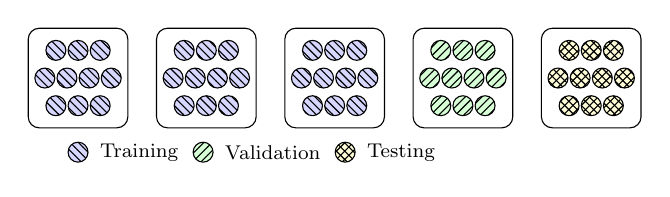
\begin{tikzpicture}[
  line width=0.4pt,
  node distance=0ex and 0em,
  every node/.style={scale=0.9},
  gridBox/.style={rectangle, opacity=0, draw=red},
  box/.style={rectangle, draw=black, inner sep=2pt, font=\small},
  rounded box/.style={rectangle, rounded corners, draw=black, inner sep=2pt, font=\small},
  anno/.style={font=\footnotesize},
]

  % legends
  \node (b-l-train) at (0, -2ex) [sExample, dsTrain] {};
  \node (b-l-train-text) [right = .1em of b-l-train] [anno] {\Train};
  \node (b-l-val) [right = .2em of b-l-train-text] [sExample, dsVal] {};
  \node (b-l-val-text) [right = .1em of b-l-val] [anno] {\Val};
  \node (b-l-test) [right = .2em of b-l-val-text] [sExample, dsTest] {};
  \node (b-l-test-text) [right = .1em of b-l-test] [anno] {\Test};

  \node (b-p1) at (0,0) [anchor=south, sProject] {};
  \node (b-p2) [right = \wSepProject of b-p1.east] [sProject] {};
  \node (b-p3) [right = \wSepProject of b-p2.east] [sProject] {};
  \node (b-p4) [right = \wSepProject of b-p3.east] [sProject] {};
  \node (b-p5) [right = \wSepProject of b-p4.east] [sProject] {};

  \foreach \pi/\ds in {1/dsTrain,2/dsTrain,3/dsTrain,4/dsVal,5/dsTest} {
    \foreach \ex/\ey [count=\ei] in {
      -.8em/-1em, 0em/-1em, .8em/-1em,
      -1.2em/0, -.4em/0, .4em/0, 1.2em/0,
      -.8em/1em, 0em/1em, .8em/1em
    } {
      \node (b-p\pi-\ei) [below right = \ey and \ex of b-p\pi.center, anchor=center] [sExample, \ds] {};
    }
  };

\end{tikzpicture}

  \caption{\Crossproj \methodology. \label{fig:method-crossproj}}
\end{figure}

The \emph{\crossproj} methodology extracts examples at a single point
in time from various projects.  This methodology was also commonly
used in prior work.  Unlike the \mixedproj \methodology, \crossproj
splits the \emph{set of projects} into testing, validation, and
training sets.  Thus, all \examples from any project in the
training/validation/testing set will be used for
training/validation/testing.\Fix{This sounds like mixed project. Shouldn't it be the set of projects in test/val is disjoint from those in train?}
%
Figure~\ref{fig:method-crossproj} illustrates this
methodology\Fix{gray}.  More formally, we define the following sets:
%
\begin{align*}
  \aprojecttrain, \aprojectval, \aprojecttest = \asplit(\ashuffle(P), x, y, z) \\
  \atrain = \bigcup_{\aproject \in \aprojecttrain} \aextract(\atime, \aproject) \\
  \aval = \bigcup_{\aproject \in \aprojectval} \aextract(\atime, \aproject) \\
  \atest = \bigcup_{\aproject \in \aprojecttest} \aextract(\atime, \aproject)
\end{align*}
%
The \crossproj methodology is explicitly testing the ability to
transfer a model to new projects.
%
However, \crossproj is also time-unaware, i.e., it does not consider
if \examples from a project that is in testing set come before or
after \examples from projects in the training set.

% I would be surprised if it made a difference since this would imply
% causal contamination across projects which is possible but I assume
% unlikely.

\subsection{\Evoaware}

\begin{figure}[t]
  \centering
  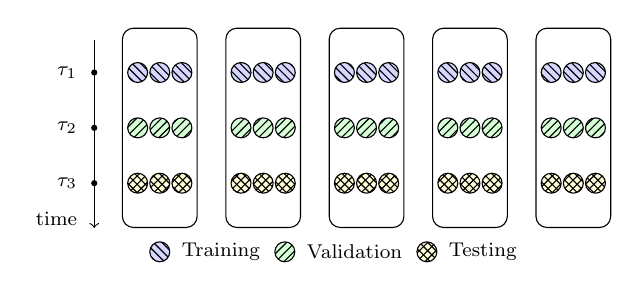
\begin{tikzpicture}[
  line width=0.4pt,
  node distance=0ex and 0em,
  every node/.style={scale=0.9},
  gridBox/.style={rectangle, opacity=0, draw=red},
  box/.style={rectangle, draw=black, inner sep=2pt, font=\small},
  rounded box/.style={rectangle, rounded corners, draw=black, inner sep=2pt, font=\small},
  anno/.style={font=\footnotesize},
]

  % legends
  \node (b-l-train) at (0, -2ex) [sExample, dsTrain] {};
  \node (b-l-train-text) [right = .1em of b-l-train] [anno] {\Train};
  \node (b-l-val) [right = .2em of b-l-train-text] [sExample, dsVal] {};
  \node (b-l-val-text) [right = .1em of b-l-val] [anno] {\Val};
  \node (b-l-test) [right = .2em of b-l-val-text] [sExample, dsTest] {};
  \node (b-l-test-text) [right = .1em of b-l-test] [anno] {\Test};

  \tikzset{sEvoProject/.style={sProject, minimum height=8em, minimum width=3em}}

  \node (b-p1) at (0,0) [anchor=south,sEvoProject] {};
  \node (b-p2) [right = \wSepProject of b-p1.east] [sEvoProject] {};
  \node (b-p3) [right = \wSepProject of b-p2.east] [sEvoProject] {};
  \node (b-p4) [right = \wSepProject of b-p3.east] [sEvoProject] {};
  \node (b-p5) [right = \wSepProject of b-p4.east] [sEvoProject] {};

  \node[coordinate] (c-time-beg) [below left = 1ex and 1em of b-p1.north west] {};
  \node[coordinate] (c-time-end) [above left = 0ex and 1em of b-p1.south west] {};
  \draw[->] (c-time-beg) -- (c-time-end);
  \node (b-time) [above left = -.5ex and .3em of c-time-end] [anno] {time};

  \foreach \pi in {1,2,3,4,5} {
    \foreach \ex/\ey/\ds [count=\ei] in {
      -.8em/-2em/dsTrain, 0em/-2em/dsTrain, .8em/-2em/dsTrain,
      -.8em/0/dsVal,  0em/0/dsVal, .8em/0/dsVal,
      -.8em/2em/dsTest, 0em/2em/dsTest, .8em/2em/dsTest} {
      \node (b-p\pi-\ei) [below right = \ey and \ex of b-p\pi.center, anchor=center] [sExample, \ds] {};
    }
  };

  \node (b-t1) at (c-time-beg |- b-p1-1) [circle, minimum size=.2em, inner sep=0, draw=black, fill=black] {};
  \node (b-t1-text) [left = .2em of b-t1] [anno] {$\tau_1$};
  \node (b-t2) at (c-time-beg |- b-p1-4) [circle, minimum size=.2em, inner sep=0, draw=black, fill=black] {};
  \node (b-t2-text) [left = .2em of b-t2] [anno] {$\tau_2$};
  \node (b-t3) at (c-time-beg |- b-p1-7) [circle, minimum size=.2em, inner sep=0, draw=black, fill=black] {};
  \node (b-t3-text) [left = .2em of b-t3] [anno] {$\tau_3$};

\end{tikzpicture}

  \caption{\Evoaware \methodology. \label{fig:method-evoaware}}
\end{figure}

We propose a novel \methodology, dubbed \emph{\evoaware}.  Unlike the
\methodologies explained earlier in this section, the \evoaware
\methodology is \emph{time-aware}, i.e., \examples in the training set
were available in software repositories \emph{before} \examples in the
validation set, which were in turn available \emph{before} examples in
the testing set.  Figure~\ref{fig:method-evoaware} illustrates this
\methodology.  This \methodology could be used in combination with
\mixedproj or \crossproj.  More formally, we define the following
steps: \JiyangComment{Do we want to introduce filter function here?}
\begin{align*}
  \atrain = \bigcup_{\aproject \in projects} \aextract(\atime^{-2}, \aproject) \\
  \aval = \bigcup_{\aproject \in projects} \aextract(\atime^{-1}, \aproject) \setminus \atrain \\
  \atest = \bigcup_{\aproject \in projects} \aextract(\atime, \aproject) \setminus \atrain \setminus \aval \\
\end{align*}

\section{Use Cases}
\label{sec:use:cases}

As we saw in the previous section, \methodologies are used to set up
experiments and obtain an appropriate dataset for the evaluation.
However, \methodologies do \emph{not} describe the envisioned use of a
model.  Prior work focused on \methodologies, but we argue that
proposed models should be described in terms of \emph{use cases},
i.e., how will the developers use the models eventually.  Once a use
case is chosen, an appropriate \methodology can be selected to
evaluate the model.

% when a model might (not) be used.  Prior work focused on
%\methodologies, but we argue that models should on \emph{use cases}.

In this section, we define three use cases.  The first two use cases
are ``extracted'' from prior work (described in the previous section).
Namely, we reasoned about the evaluation \methodologies that were used
and tried to link it to (somewhat) practical use cases.  The third use
case that we describe is inspired by our own development and can be
evaluated using the \evoaware \methodology.  Note that we do not try
to provide an exhaustive list of use cases, but rather to start off
this important distinction between a use case and an evaluation
\methodology.  We will introduce the use cases via examples.

\Fix{After reading this section: I like (C) and I buy the arguments, but first reading (A) and (B) is quite confusing to me.}

% in what ways developers might end up using
%code summarization models.  We also discuss what methodology is the
%most appropriate to be used to obtain a dataset for evaluating models
%in each use case.  Note that our goal is not to provide an exhaustive
%list of use cases, but to highlight that the use cases should play an
%important role when choosing the evaluation methodology and reporting
%the findings in research papers.

\subsection{In-Project Batch Use Case}

Consider Alice, a developer at a large software company.  Alice has
been developing several features in her project over extended period
of time (since \atimep), but she had no chance to write comments for
all her code.  At one point (\atime), she decided it was time to
document methods without comments.  
\Fix{Doesn't the mixed methodology require also some training data 
within the current project?}
She wants to use an ML model that
can automatically generate comments.  Alice decides to train a model
using already existing \examples (i.e., existing method and comment
pairs) in her code and \examples (available at time \atime) from
several projects on GitHub.  We call this \emph{\ipmode batch use
  case}, because Alice trains a new model every time she wants to use
the model, and she applies it to several methods.  This use case can
be evaluated using the \mixedproj \methodology.

Prior work that used the \mixedproj \methodology
(Table~\ref{table:prior-work}) could fit under this use case, but only
if we assume that some methods have not been documented for very long
time, i.e., $\atime - \atimep = \infty$.
\Fix{Why? Isn't it always feasible to apply this methodology at any point when you need to generate one? Or does the infinity refer to time here?s}
%% \JiyangComment{I think this use case is not 100 percent
%%   consistent with what prior work do. Because you mention at time $t$
%%   Alice want to train the model so that the model can not be trained
%%   using the future data. However, the prior work does not consider
%%   time, they only use the data available at time t and then split.
%%   Should we add that without considering time, prior work is
%%   incorrect?}
% Milos: Note that examples that she wants to document are included
% *before* $t$ (and potentially long time before $t$).

\subsection{Cross-Project Batch Use Case}

In this case, we assume that Alice works on a project (since \atimep)
without writing any documentation for her code.
%
At some point (\atime), Alice decides to document all her methods.
Again, she wants to use an ML model to help her get the task done.
Since Alice does not have any comments in her code, she decides to
only train on projects available on GitHub (at time \atime).  She uses
all \examples (i.e., pairs of methods and comments) in the training
and sets a couple of projects aside for validation.
%
Once the model is trained, she uses it to generate comments for all
the methods that she has.  We call this \emph{\pmode batch use case},
because Alice trains a new model at a specific time point and applies
it to all the methods she has.  (Note that once she integrates the
comments that she likes, she can use them in the future, which matches
\ipmode batch use case, or potentially she could decide to ignore
those comments and always generates new comments, but this is highly
unlikely.)  This use case can be evaluated using the \crossproj
\methodology.

Prior work that used \crossproj (Table~\ref{table:prior-work}) could
fit under this use case, under the assumption that the comment has not
been documented for very long time, i.e., $\atime - \atimep = \infty$.
\Fix{Same question as above: I don't see the case for infinity. PN: how about $\atime - \atimep \rightarrow \infty$}

%% \JiyangComment{Same question here, Alice also considers time when
%%   training the model. It is possible that prior work use the new
%%   project say created in 2019 to train and test in project that is
%%   created in 2012.}

\subsection{Continuous Use Case}

In this case, Alice writes documentation for each method around the
same time as the method itself.  For example, Alice might integrate a
model for comment generation into her IDE that would suggest comments
once Alice indicates that a method is complete.  (Updating and
maintaining comments as code
evolves~\cite{PanthaplackelETAL20CommentUpdate} is an important topic,
but orthogonal to our work.)  Before using the model at \atime, Alice
would have to train the model on the data available in her project and
other projects at \atimep.  She can keep using the same model for as
long as she wishes (i.e., $\atime-\atimep$ can be arbitrary large).
We call this \emph{\cmode}, because the only data that can be used to
train the model is the data from past.  This use case can be evaluated
using the \evoaware \methodology.

The model should be retrained once in a while, e.g., when a new Java
version is introduced that adds new syntax into the language and
developers start adopting the syntax.  Finding an appropriate
frequency at which to retrain the model is left for future work.

\section{Experiment Setup}
\label{sec:settings}

In this section, we describe our experiment setup for comparing the
\methodologies.  This setup is generic and could be used for any task.
%
In this work we instantiate it for \comgen and \methnam tasks.  
\Fix{In the intro you said you do two code summarization tasks.}
The
goal of the experiment is to train a model following each \methodology
and evaluate and compare the models on a \emph{test set that is
  common} to all \methodologies.  We record automatic metrics and
reason about their differences.  \Fix{no prior work used human eval}

We define notations, by extending Section~\ref{sec:prelim}, to help us
accurately describe our experiment setup.  Let $\mathcal{P}$ be the
set of projects we intend to collect data from.  We then perform the
split $\mathcal{P}_{train}, \mathcal{P}_{val}, \mathcal{P}_{test} =
\asplit(\mathcal{P}, 80\%, 10\%, 10\%)$.  The ratio of 80\%/10\%/10\%
is chosen following machine learning common
practice~\cite{StanfordSplitting}.

Let $\mathcal{D}(\mathcal{P}, \atime) = \sum_{P\in\mathcal{P}}
\aextract(\atime, P)$ be the data collected from projects in
$\mathcal{P}$ at time point $t$.  The exact implementation of
$\mathcal{D}(\cdot, \cdot)$ is task-specific.

Let $\mathcal{D}(\mathcal{P}, \atimep, \atime)$ be the new data from
projects in $\mathcal{P}$ after time point \atimep{} before time point
\atime{}.  To compute $\mathcal{D}(Set[Project], Time, Time)$, let
$F(d_1, d_2)$ be a \filterfunc that returns a subset of $d_2$ after
removing the data exists in $d_1$.  The exact implementation of
$F(Set, Set)$ is task-specific.  Then, we have
$\mathcal{D}(\mathcal{P}, \atimep, \atime) =
F(\mathcal{D}(\mathcal{P}, \atimep), \mathcal{D}(\mathcal{P},
\atime))$.

Given $\mathcal{D}(\mathcal{P}, \atime)$ and $\mathcal{D}(\mathcal{P},
\atimep, \atime)$, we perform the splits:
\begin{flalign*}
  &\mathcal{D}_{train}(\mathcal{P}, \atime), \mathcal{D}_{val}(\mathcal{P}, \atime), \mathcal{D}_{test}(\mathcal{P}, \atime) \\
  &\quad = \asplit(\mathcal{D}(\mathcal{P}, \atime), 80\%, 10\%, 10\%) \\
%
  &\mathcal{D}_{train}(\mathcal{P}, \atimep, \atime), \mathcal{D}_{val}(\mathcal{P}, \atimep, \atime), \mathcal{D}_{test}(\mathcal{P}, \atimep, \atime) \\
  &\quad = \asplit(\mathcal{D}(\mathcal{P}, \atimep, \atime), 80\%, 10\%, 10\%)
\end{flalign*}
of the data respectively, and ensures that
$$
\forall x \in \{train, val, test\}, \mathcal{D}_x(\mathcal{P}, \atimep, \atime) \subseteq \mathcal{D}_x(\mathcal{P}, \atime)
$$

\begin{figure*}[t]
  \centering
  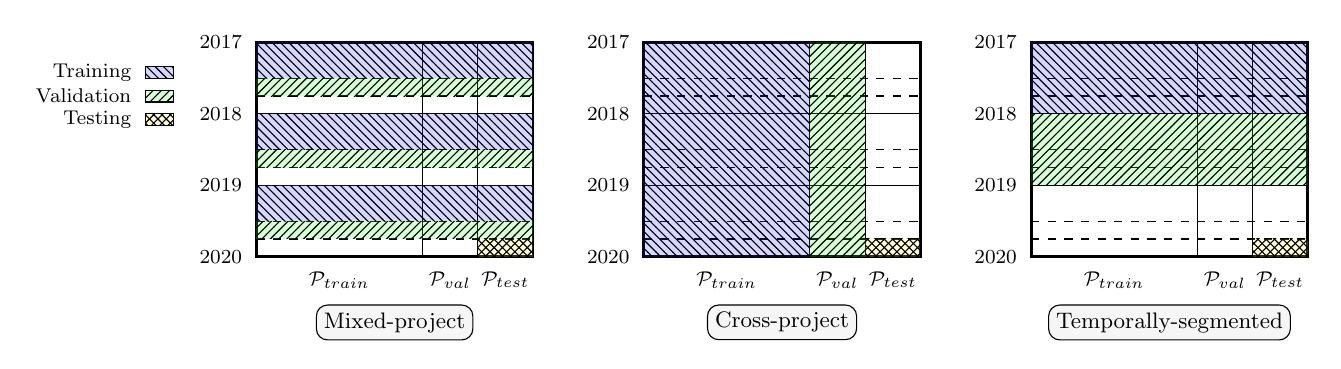
\begin{tikzpicture}[
  line width=0.4pt,
  node distance=0ex and 0em,
  every node/.style={scale=0.9},
  gridBox/.style={rectangle, opacity=0, draw=red},
  box/.style={rectangle, draw=black, inner sep=2pt, font=\small},
  rounded box/.style={rectangle, rounded corners, draw=black, fill=gray!20, inner sep=3pt, font=\small},
  anno/.style={font=\footnotesize},
]

  % legends

  \draw[dsTrain] (-4em,-2ex) rectangle (-3em,-3ex);
  \node (b-l-train) at (-4.2em,-2.5ex) [anchor=east, anno] {\Train};
  \draw[dsVal] (-4em,-4ex) rectangle (-3em,-5ex);
  \node (b-l-val) at (-4.2em,-4.5ex) [anchor=east, anno] {\Val};
  \draw[dsTest] (-4em,-6ex) rectangle (-3em,-7ex);
  \node (b-l-test) at (-4.2em,-6.5ex) [anchor=east, anno] {\Test};
  

  \foreach \s/\xbase in {mixedproj/0,crossproj/14em,evoaware/28em} {
    
    \node[coordinate] (\s-p1) at (\xbase,0) [] {};
    \node[coordinate] (\s-p2) [right = 6em of \s-p1] [] {};
    \node[coordinate] (\s-p3) [right = 8em of \s-p1] [] {};
    \node[coordinate] (\s-p4) [right = 10em of \s-p1] [] {};

    \node[coordinate] (\s-t1) at (\xbase,0) [] {};
    \node[coordinate] (\s-t2) [below = 6ex of \s-t1] [] {};
    \node[coordinate] (\s-t3) [below = 12ex of \s-t1] [] {};
    \node[coordinate] (\s-t4) [below = 18ex of \s-t1] [] {};

    \foreach \x/\y in {1/2,2/3,3/4} {
      \node[coordinate] (\s-t\x-1) at ($(\s-t\x)!0.5!(\s-t\y)$) [] {};
      \node[coordinate] (\s-t\x-2) at ($(\s-t\x)!0.75!(\s-t\y)$) [] {};
    };

    \foreach \x/\t in {1/2017,2/2018,3/2019,4/2020} {
      \node (\s-b-t\x) [left = .2em of \s-t\x] [anno] {\t};
    };

    \draw[line width=1pt] (\s-p4) rectangle (\s-t4);

    \foreach \x in {2,3} {
      \draw (\s-t1 -| \s-p\x) -- (\s-t4 -| \s-p\x);
    };

    \foreach \x in {2,3} {
      \draw (\s-t\x -| \s-p1) -- (\s-t\x -| \s-p4);
    };

    \foreach \x in {1-1,1-2,2-1,2-2,3-1,3-2} {
      \draw[dashed] (\s-t\x -| \s-p1) -- (\s-t\x -| \s-p4);
    }

    \node[coordinate] (\s-p1-base) at ($(\s-p1|-\s-t4)!0.5!(\s-p2|-\s-t4)$) [] {};
    \node[coordinate] (\s-p2-base) at ($(\s-p2|-\s-t4)!0.5!(\s-p3|-\s-t4)$) [] {};
    \node[coordinate] (\s-p3-base) at ($(\s-p3|-\s-t4)!0.5!(\s-p4|-\s-t4)$) [] {};
    \foreach \x/\ds in {1/train,2/val,3/test} {
      \node (\s-b-p\x) [below = .5ex of \s-p\x-base] [anno] {$\mathcal{P}_{\ds}$};
    };

    \node[coordinate] (\s-south) at ($(\s-p1|-\s-t4)!0.5!(\s-p4|-\s-t4)$) [] {};
  };

  \node (mixedproj-b-text) [below = 4ex of mixedproj-south] [rounded box] {\Mixedproj};
  \node (crossproj-b-text) [below = 4ex of crossproj-south] [rounded box] {\Crossproj};
  \node (evoaware-b-text) [below = 4ex of evoaware-south] [rounded box] {\Evoaware};

  \foreach \x in {1,2,3} {
    \draw[dsTrain, draw=none] (mixedproj-p1|-mixedproj-t\x) rectangle (mixedproj-p4|-mixedproj-t\x-1);
    \draw[dsVal, draw=none] (mixedproj-p1|-mixedproj-t\x-1) rectangle (mixedproj-p4|-mixedproj-t\x-2);
  }
  \draw[dsTest, draw=none] (mixedproj-p4|-mixedproj-t3-2) rectangle (mixedproj-p3|-mixedproj-t4);

  \draw[dsTrain, draw=none] (crossproj-p2) rectangle (crossproj-p1|-crossproj-t4);
  \draw[dsVal, draw=none] (crossproj-p3) rectangle (crossproj-p2|-crossproj-t4);
  \draw[dsTest, draw=none] (crossproj-p4|-crossproj-t3-2) rectangle (crossproj-p3|-crossproj-t4);

  \draw[dsTrain, draw=none] (evoaware-p1|-evoaware-t1) rectangle (evoaware-p4|-evoaware-t2);
  \draw[dsVal, draw=none] (evoaware-p1|-evoaware-t2) rectangle (evoaware-p4|-evoaware-t3);
  \draw[dsTest, draw=none] (evoaware-p4|-evoaware-t3-2) rectangle (evoaware-p3|-evoaware-t4);

\end{tikzpicture}

  \caption{Evaluation settings. \JiyangComment{It is a bit confusing
      to include time for Mixed-project, I suggest removing time in y
      axis.}\label{fig:eval-settings}}
\end{figure*}

\InputWithSpace{tables/table-eval-settings}

For each \methodology, we design an evaluation setting that specifies
the examples used for \train, \val, and \test.
Figure~\ref{fig:eval-settings} illustrates the \train, \val, and \test
sets for each \methodology, and Table~\ref{table:eval-settings} lists
those sets using the notations we just defined.  $\atimeppp, \atimepp,
\atimep, \atime$ are the chronologically ordered time points at which
we collect the \dataset{s}; in our experiment, we choose $\atimeppp =
\ajanone, 2017; \atimepp = \ajanone, 2018; \atimep = \ajanone, 2019;
\atime = \ajanone, 2020$.

For the \mixedproj \methodology, we use all examples available at
$\atime$ and split them into \train, \val, and \test sets, and
examples in different sets are allowed to come from the same project.
For the \crossproj \methodology, we still use all examples available
at $\atime$ but ensure that examples of one project can be only in one
of \train, \val, or \test set.  For the \evoaware \methodology, we use
the examples between $\atimeppp$ and $\atimepp$ for \train, between
$\atimepp$ and $\atimep$ for \val, and between $\atimep$ and $\atime$
for \test. Specially, the \test set is constrained in a way that only
contains examples that fit all the three \methodologies.

%% The \test sets of the three settings are by natural different, which
%% makes it hard to compare different evaluation settings using the same
%% model and the same metric.  To compare the three evaluation settings
%% in a controlled way, we take the union of their \test sets as the
%% \textit{\common} \test set (denote as $T_{\common}$).  We will refer
%% to the \test set that are specific to each evaluation setting as the
%% \textit{\standard} \test set (denote as $T_{\standard}$).
%% Table~\ref{table:eval-settings} lists the \train, \val, and \standard
%% \test sets for each evaluation setting, as well as the \common \test
%% set.  For simplicity, we use the 4-digits year to represent the time
%% point at the beginning of that year, e.g., 2020 represents Jan 1, 2020
%% 00:00.

%% # Use cases

%% ## Evolution
%% - Train on Data(P_train, 2017, 2018), validation on Data(P_val, 2018, 2019);
%% - Test on Data_test(P_test, 2019, 2020);

%% ## Cross-project
%% - Train on Data(P_train, 2020), validation on Data(P_val, 2020);
%% - Test on Data_test(P_test, 2019, 2020);
%% - Optionally test on Data(P_test, 2020) and show the results are not statistically significantly different than testing on the previous test set;

%% ## Mixed-project
%% - Train on Data_train(P, 2020), validation on Data_val(P, 2020);
%% - Test on Data_test(P_test, 2019, 2020);
%% - Optionally test on Data_test(P, 2020) and show the results are not statistically significantly different than testing on the previous test set;

\section{Dataset}
\label{sec:data}

This section describes the dataset we collected to facilitate our
experiments.  We collected our dataset as mappings between code and
natural language elements from large and popular evolving projects.
For our tasks, we extract methods (as code elements) and method names
and \javadoc comments as natural language elements.  In our study, we
chose to use only projects written in the Java programming language,
because \Fix{most/all} prior work focused on this language.  We also
focus only on comments that are written in English to be consistent
with prior work.  In the future, it would be worth studying other
programming and natural languages.

%The code is Java methods, and the natural language elements are the
%names and \javadoc comments of those methods.

We started with the \NumProjectPlanned Java projects on GitHub that
have the most stars (i.e., most number of users who liked the
projects).  This approach was used in \Fix{most} recent related work.
We then discarded the projects where no valid data could be collected
(e.g., no method \javadoc) or are obviously not software projects
(e.g.,
\href{https://github.com/CyC2018/CS-Notes}{CyC2018/CS-Notes}). After
this filtering, we ended up with \NumProject projects.  For each
project, we then performed the following steps:
\begin{enumerate}
\item clone the project;
\item checkout revisions on \ajanone{} of each year from 2017 to 2020;
\item at each revision, find all \CodeIn{*.java} files and use
  JavaParser~\cite{JavaParser} to parse the files;
\item collect all method bodies (removing inline comments from them)
  and their \javadoc, but discarding the data that matches any of the
  following conditions: (a) the method is abstract; (b) the \javadoc
  summary is empty; (c) the method body or the \javadoc summary
  contains non-English characters; (d) the method body is longer than
  10,000 characters.\Fix{how many for each}
\end{enumerate}

The final dataset consists of \NumDataAll unique method-\javadoc pairs
across all \NumRevisionAll revisions (\NumDataLatest from the latest
revision at \ajanone{}, 2020).

We implement the \filterfunc $F(d_1, d_2)$ to keep only the new
methods in $d_2$ that do not exist in $d_1$, by removing the method
that has the same tuple of class name, method name, and method
arguments:
\begin{flalign*}
  &F(d_1, d_2) = \{ m | m \in d_2 \land \lqall{m' \in d_1} \\
  &\qquad (\mathtt{ClassName}(m), \mathtt{Name}(m), \mathtt{Arguments}(m)) \neq \\
  &\qquad\qquad (\mathtt{ClassName}(m'), \mathtt{Name}(m'), \mathtt{Arguments}(m'))\}
\end{flalign*}

\input{tables/table-CG-dataset-metrics-main}

%% Automatically generated by pyutil.latex 

\begin{table}
\begin{small}
\begin{center}
\caption{\TCDatasetMetricsMainMN}
\begin{tabular}{ l@{\hspace{2pt}}|@{\hspace{2pt}}c@{\hspace{2pt}} | r r r}
\toprule
\multicolumn{2}{c|}{} & & & \\
\multicolumn{2}{c|}{\multirow{-2}{*}{\THDSStat}} & \multirow{-2}{*}{\UseMacro{TH-ds-all}} & \multirow{-2}{*}{\UseMacro{TH-ds-2020}} & \multirow{-2}{*}{\UseMacro{TH-ds-2019-2020}} \\
\midrule
\multicolumn{2}{c|}{\UseMacro{TH-ds-num-project}}
 & \UseMacro{ds-MN-num-proj}
 & \UseMacro{ds-MN-num-proj}
 & \UseMacro{ds-MN-num-proj}
\\
\multicolumn{2}{c|}{\UseMacro{TH-ds-num-data}}
 & \UseMacro{raw-ds-MN-num-data_all}
 & \UseMacro{ds-MN-num-data_2020}
 & \UseMacro{ds-MN-num-data_2019-2020}
\\
\midrule
& \UseMacro{TH-ds-len-method-avg}
 & \UseMacro{raw-ds-MN-len-meth-AVG_all}
 & \UseMacro{ds-MN-len-meth-AVG_2020}
 & \UseMacro{ds-MN-len-meth-AVG_2019-2020}
\\
& \UseMacro{TH-ds-len-method-mode}
 & \UseMacro{raw-ds-MN-len-meth-MODE_all}
 & \UseMacro{ds-MN-len-meth-MODE_2020}
 & \UseMacro{ds-MN-len-meth-MODE_2019-2020}
\\
& \UseMacro{TH-ds-len-method-median}
 & \UseMacro{raw-ds-MN-len-meth-MEDIAN_all}
 & \UseMacro{ds-MN-len-meth-MEDIAN_2020}
 & \UseMacro{ds-MN-len-meth-MEDIAN_2019-2020}
\\
& \UseMacro{TH-ds-len-method-le100}
 & \UseMacro{raw-ds-MN-len-meth-le-100_all}
 & \UseMacro{ds-MN-len-meth-le-100_2020}
 & \UseMacro{ds-MN-len-meth-le-100_2019-2020}
\\
& \UseMacro{TH-ds-len-method-le150}
 & \UseMacro{raw-ds-MN-len-meth-le-150_all}
 & \UseMacro{ds-MN-len-meth-le-150_2020}
 & \UseMacro{ds-MN-len-meth-le-150_2019-2020}
\\
\multirow{-6}{*}{\UseMacro{TH-ds-len-method}} & \UseMacro{TH-ds-len-method-le200}
 & \UseMacro{raw-ds-MN-len-meth-le-200_all}
 & \UseMacro{ds-MN-len-meth-le-200_2020}
 & \UseMacro{ds-MN-len-meth-le-200_2019-2020}
\\
\midrule
& \UseMacro{TH-ds-len-comment-avg}
 & \UseMacro{raw-ds-MN-len-com-AVG_all}
 & \UseMacro{ds-MN-len-com-AVG_2020}
 & \UseMacro{ds-MN-len-com-AVG_2019-2020}
\\
& \UseMacro{TH-ds-len-comment-mode}
 & \UseMacro{raw-ds-MN-len-com-MODE_all}
 & \UseMacro{ds-MN-len-com-MODE_2020}
 & \UseMacro{ds-MN-len-com-MODE_2019-2020}
\\
& \UseMacro{TH-ds-len-comment-median}
 & \UseMacro{raw-ds-MN-len-com-MEDIAN_all}
 & \UseMacro{ds-MN-len-com-MEDIAN_2020}
 & \UseMacro{ds-MN-len-com-MEDIAN_2019-2020}
\\
& \UseMacro{TH-ds-len-comment-le20}
 & \UseMacro{raw-ds-MN-len-com-le-20_all}
 & \UseMacro{ds-MN-len-com-le-20_2020}
 & \UseMacro{ds-MN-len-com-le-20_2019-2020}
\\
& \UseMacro{TH-ds-len-comment-le30}
 & \UseMacro{raw-ds-MN-len-com-le-30_all}
 & \UseMacro{ds-MN-len-com-le-30_2020}
 & \UseMacro{ds-MN-len-com-le-30_2019-2020}
\\
\multirow{-6}{*}{\UseMacro{TH-ds-len-comment}} & \UseMacro{TH-ds-len-comment-le50}
 & \UseMacro{raw-ds-MN-len-com-le-50_all}
 & \UseMacro{ds-MN-len-com-le-50_2020}
 & \UseMacro{ds-MN-len-com-le-50_2019-2020}
\\
\midrule
& \UseMacro{TH-ds-len-name-avg}
 & \UseMacro{raw-ds-MN-len-name-AVG_all}
 & \UseMacro{ds-MN-len-name-AVG_2020}
 & \UseMacro{ds-MN-len-name-AVG_2019-2020}
\\
& \UseMacro{TH-ds-len-name-mode}
 & \UseMacro{raw-ds-MN-len-name-MODE_all}
 & \UseMacro{ds-MN-len-name-MODE_2020}
 & \UseMacro{ds-MN-len-name-MODE_2019-2020}
\\
& \UseMacro{TH-ds-len-name-median}
 & \UseMacro{raw-ds-MN-len-name-MEDIAN_all}
 & \UseMacro{ds-MN-len-name-MEDIAN_2020}
 & \UseMacro{ds-MN-len-name-MEDIAN_2019-2020}
\\
& \UseMacro{TH-ds-len-name-le2}
 & \UseMacro{raw-ds-MN-len-name-le-3_all}
 & \UseMacro{ds-MN-len-name-le-3_2020}
 & \UseMacro{ds-MN-len-name-le-3_2019-2020}
\\
& \UseMacro{TH-ds-len-name-le3}
 & \UseMacro{raw-ds-MN-len-name-le-5_all}
 & \UseMacro{ds-MN-len-name-le-5_2020}
 & \UseMacro{ds-MN-len-name-le-5_2019-2020}
\\
\multirow{-6}{*}{\UseMacro{TH-ds-len-name}} & \UseMacro{TH-ds-len-name-le6}
 & \UseMacro{raw-ds-MN-len-name-le-6_all}
 & \UseMacro{ds-MN-len-name-le-6_2020}
 & \UseMacro{ds-MN-len-name-le-6_2019-2020}
\\
\bottomrule
\end{tabular}
\end{center}
\end{small}
\vspace{\TVDatasetMetricsMainMN}
\end{table}

\input{tables/table-CG-dataset-metrics-split}

%% Automatically generated by pyutil.latex 

\begin{table*}
\begin{small}
\begin{center}
\caption{\TCDatasetMetricsSplitMN}
\begin{tabular}{ l@{\hspace{2pt}}|@{\hspace{2pt}}c@{\hspace{2pt}} | rr @{\hspace{5pt}}c@{\hspace{5pt}} rr @{\hspace{5pt}}c@{\hspace{5pt}} rr r}
\toprule
\multicolumn{2}{c|}{} & \multicolumn{2}{c}{\UseMacro{TH-ds-mixedproj}} & & \multicolumn{2}{c}{\UseMacro{TH-ds-crossproj}} & & \multicolumn{2}{c}{\UseMacro{TH-ds-evo}} & \\\cline{3-4}\cline{6-7}\cline{9-10}
\multicolumn{2}{c|}{\multirow{-2}{*}{\THDSStat}} & \UseMacro{TH-ds-mixedproj-train} & \UseMacro{TH-ds-mixedproj-val} & & \UseMacro{TH-ds-crossproj-train} & \UseMacro{TH-ds-crossproj-val} & & \UseMacro{TH-ds-evo-train} & \UseMacro{TH-ds-evo-val} & \multirow{-2}{*}{\UseMacro{TH-ds-test}} \\
\midrule
\multicolumn{2}{c|}{\UseMacro{TH-ds-num-project}}
 & \UseMacro{ds-MN-num-proj}
 & \UseMacro{ds-MN-num-proj}
 & 
 & \UseMacro{ds-MN-num-proj_train}
 & \UseMacro{ds-MN-num-proj_val}
 & 
 & \UseMacro{ds-MN-num-proj}
 & \UseMacro{ds-MN-num-proj}
 & \UseMacro{ds-MN-num-proj_test}
\\
\multicolumn{2}{c|}{\UseMacro{TH-ds-num-data}}
 & \UseMacro{ds-MN-num-data_mixedproj-2020-train}
 & \UseMacro{ds-MN-num-data_mixedproj-2020-val}
 & 
 & \UseMacro{ds-MN-num-data_crossproj-2020-train}
 & \UseMacro{ds-MN-num-data_crossproj-2020-val}
 & 
 & \UseMacro{ds-MN-num-data_evo-2020-train}
 & \UseMacro{ds-MN-num-data_evo-2020-val}
 & \UseMacro{ds-MN-num-data_2020-test_common}
\\
\midrule
& \UseMacro{TH-ds-len-method-avg}
 & \UseMacro{ds-MN-len-meth-AVG_mixedproj-2020-train}
 & \UseMacro{ds-MN-len-meth-AVG_mixedproj-2020-val}
 & 
 & \UseMacro{ds-MN-len-meth-AVG_crossproj-2020-train}
 & \UseMacro{ds-MN-len-meth-AVG_crossproj-2020-val}
 & 
 & \UseMacro{ds-MN-len-meth-AVG_evo-2020-train}
 & \UseMacro{ds-MN-len-meth-AVG_evo-2020-val}
 & \UseMacro{ds-MN-len-meth-AVG_2020-test_common}
\\
& \UseMacro{TH-ds-len-method-mode}
 & \UseMacro{ds-MN-len-meth-MODE_mixedproj-2020-train}
 & \UseMacro{ds-MN-len-meth-MODE_mixedproj-2020-val}
 & 
 & \UseMacro{ds-MN-len-meth-MODE_crossproj-2020-train}
 & \UseMacro{ds-MN-len-meth-MODE_crossproj-2020-val}
 & 
 & \UseMacro{ds-MN-len-meth-MODE_evo-2020-train}
 & \UseMacro{ds-MN-len-meth-MODE_evo-2020-val}
 & \UseMacro{ds-MN-len-meth-MODE_2020-test_common}
\\
& \UseMacro{TH-ds-len-method-median}
 & \UseMacro{ds-MN-len-meth-MEDIAN_mixedproj-2020-train}
 & \UseMacro{ds-MN-len-meth-MEDIAN_mixedproj-2020-val}
 & 
 & \UseMacro{ds-MN-len-meth-MEDIAN_crossproj-2020-train}
 & \UseMacro{ds-MN-len-meth-MEDIAN_crossproj-2020-val}
 & 
 & \UseMacro{ds-MN-len-meth-MEDIAN_evo-2020-train}
 & \UseMacro{ds-MN-len-meth-MEDIAN_evo-2020-val}
 & \UseMacro{ds-MN-len-meth-MEDIAN_2020-test_common}
\\
& \UseMacro{TH-ds-len-method-le100}
 & \UseMacro{ds-MN-len-meth-le-100_mixedproj-2020-train}
 & \UseMacro{ds-MN-len-meth-le-100_mixedproj-2020-val}
 & 
 & \UseMacro{ds-MN-len-meth-le-100_crossproj-2020-train}
 & \UseMacro{ds-MN-len-meth-le-100_crossproj-2020-val}
 & 
 & \UseMacro{ds-MN-len-meth-le-100_evo-2020-train}
 & \UseMacro{ds-MN-len-meth-le-100_evo-2020-val}
 & \UseMacro{ds-MN-len-meth-le-100_2020-test_common}
\\
& \UseMacro{TH-ds-len-method-le150}
 & \UseMacro{ds-MN-len-meth-le-150_mixedproj-2020-train}
 & \UseMacro{ds-MN-len-meth-le-150_mixedproj-2020-val}
 & 
 & \UseMacro{ds-MN-len-meth-le-150_crossproj-2020-train}
 & \UseMacro{ds-MN-len-meth-le-150_crossproj-2020-val}
 & 
 & \UseMacro{ds-MN-len-meth-le-150_evo-2020-train}
 & \UseMacro{ds-MN-len-meth-le-150_evo-2020-val}
 & \UseMacro{ds-MN-len-meth-le-150_2020-test_common}
\\
\multirow{-6}{*}{\UseMacro{TH-ds-len-method}} & \UseMacro{TH-ds-len-method-le200}
 & \UseMacro{ds-MN-len-meth-le-200_mixedproj-2020-train}
 & \UseMacro{ds-MN-len-meth-le-200_mixedproj-2020-val}
 & 
 & \UseMacro{ds-MN-len-meth-le-200_crossproj-2020-train}
 & \UseMacro{ds-MN-len-meth-le-200_crossproj-2020-val}
 & 
 & \UseMacro{ds-MN-len-meth-le-200_evo-2020-train}
 & \UseMacro{ds-MN-len-meth-le-200_evo-2020-val}
 & \UseMacro{ds-MN-len-meth-le-200_2020-test_common}
\\
\midrule
& \UseMacro{TH-ds-len-comment-avg}
 & \UseMacro{ds-MN-len-com-AVG_mixedproj-2020-train}
 & \UseMacro{ds-MN-len-com-AVG_mixedproj-2020-val}
 & 
 & \UseMacro{ds-MN-len-com-AVG_crossproj-2020-train}
 & \UseMacro{ds-MN-len-com-AVG_crossproj-2020-val}
 & 
 & \UseMacro{ds-MN-len-com-AVG_evo-2020-train}
 & \UseMacro{ds-MN-len-com-AVG_evo-2020-val}
 & \UseMacro{ds-MN-len-com-AVG_2020-test_common}
\\
& \UseMacro{TH-ds-len-comment-mode}
 & \UseMacro{ds-MN-len-com-MODE_mixedproj-2020-train}
 & \UseMacro{ds-MN-len-com-MODE_mixedproj-2020-val}
 & 
 & \UseMacro{ds-MN-len-com-MODE_crossproj-2020-train}
 & \UseMacro{ds-MN-len-com-MODE_crossproj-2020-val}
 & 
 & \UseMacro{ds-MN-len-com-MODE_evo-2020-train}
 & \UseMacro{ds-MN-len-com-MODE_evo-2020-val}
 & \UseMacro{ds-MN-len-com-MODE_2020-test_common}
\\
& \UseMacro{TH-ds-len-comment-median}
 & \UseMacro{ds-MN-len-com-MEDIAN_mixedproj-2020-train}
 & \UseMacro{ds-MN-len-com-MEDIAN_mixedproj-2020-val}
 & 
 & \UseMacro{ds-MN-len-com-MEDIAN_crossproj-2020-train}
 & \UseMacro{ds-MN-len-com-MEDIAN_crossproj-2020-val}
 & 
 & \UseMacro{ds-MN-len-com-MEDIAN_evo-2020-train}
 & \UseMacro{ds-MN-len-com-MEDIAN_evo-2020-val}
 & \UseMacro{ds-MN-len-com-MEDIAN_2020-test_common}
\\
& \UseMacro{TH-ds-len-comment-le20}
 & \UseMacro{ds-MN-len-com-le-20_mixedproj-2020-train}
 & \UseMacro{ds-MN-len-com-le-20_mixedproj-2020-val}
 & 
 & \UseMacro{ds-MN-len-com-le-20_crossproj-2020-train}
 & \UseMacro{ds-MN-len-com-le-20_crossproj-2020-val}
 & 
 & \UseMacro{ds-MN-len-com-le-20_evo-2020-train}
 & \UseMacro{ds-MN-len-com-le-20_evo-2020-val}
 & \UseMacro{ds-MN-len-com-le-20_2020-test_common}
\\
& \UseMacro{TH-ds-len-comment-le30}
 & \UseMacro{ds-MN-len-com-le-30_mixedproj-2020-train}
 & \UseMacro{ds-MN-len-com-le-30_mixedproj-2020-val}
 & 
 & \UseMacro{ds-MN-len-com-le-30_crossproj-2020-train}
 & \UseMacro{ds-MN-len-com-le-30_crossproj-2020-val}
 & 
 & \UseMacro{ds-MN-len-com-le-30_evo-2020-train}
 & \UseMacro{ds-MN-len-com-le-30_evo-2020-val}
 & \UseMacro{ds-MN-len-com-le-30_2020-test_common}
\\
\multirow{-6}{*}{\UseMacro{TH-ds-len-comment}} & \UseMacro{TH-ds-len-comment-le50}
 & \UseMacro{ds-MN-len-com-le-50_mixedproj-2020-train}
 & \UseMacro{ds-MN-len-com-le-50_mixedproj-2020-val}
 & 
 & \UseMacro{ds-MN-len-com-le-50_crossproj-2020-train}
 & \UseMacro{ds-MN-len-com-le-50_crossproj-2020-val}
 & 
 & \UseMacro{ds-MN-len-com-le-50_evo-2020-train}
 & \UseMacro{ds-MN-len-com-le-50_evo-2020-val}
 & \UseMacro{ds-MN-len-com-le-50_2020-test_common}
\\
\midrule
& \UseMacro{TH-ds-len-name-avg}
 & \UseMacro{ds-MN-len-name-AVG_mixedproj-2020-train}
 & \UseMacro{ds-MN-len-name-AVG_mixedproj-2020-val}
 & 
 & \UseMacro{ds-MN-len-name-AVG_crossproj-2020-train}
 & \UseMacro{ds-MN-len-name-AVG_crossproj-2020-val}
 & 
 & \UseMacro{ds-MN-len-name-AVG_evo-2020-train}
 & \UseMacro{ds-MN-len-name-AVG_evo-2020-val}
 & \UseMacro{ds-MN-len-name-AVG_2020-test_common}
\\
& \UseMacro{TH-ds-len-name-mode}
 & \UseMacro{ds-MN-len-name-MODE_mixedproj-2020-train}
 & \UseMacro{ds-MN-len-name-MODE_mixedproj-2020-val}
 & 
 & \UseMacro{ds-MN-len-name-MODE_crossproj-2020-train}
 & \UseMacro{ds-MN-len-name-MODE_crossproj-2020-val}
 & 
 & \UseMacro{ds-MN-len-name-MODE_evo-2020-train}
 & \UseMacro{ds-MN-len-name-MODE_evo-2020-val}
 & \UseMacro{ds-MN-len-name-MODE_2020-test_common}
\\
& \UseMacro{TH-ds-len-name-median}
 & \UseMacro{ds-MN-len-name-MEDIAN_mixedproj-2020-train}
 & \UseMacro{ds-MN-len-name-MEDIAN_mixedproj-2020-val}
 & 
 & \UseMacro{ds-MN-len-name-MEDIAN_crossproj-2020-train}
 & \UseMacro{ds-MN-len-name-MEDIAN_crossproj-2020-val}
 & 
 & \UseMacro{ds-MN-len-name-MEDIAN_evo-2020-train}
 & \UseMacro{ds-MN-len-name-MEDIAN_evo-2020-val}
 & \UseMacro{ds-MN-len-name-MEDIAN_2020-test_common}
\\
& \UseMacro{TH-ds-len-name-le2}
 & \UseMacro{ds-MN-len-name-le-3_mixedproj-2020-train}
 & \UseMacro{ds-MN-len-name-le-3_mixedproj-2020-val}
 & 
 & \UseMacro{ds-MN-len-name-le-3_crossproj-2020-train}
 & \UseMacro{ds-MN-len-name-le-3_crossproj-2020-val}
 & 
 & \UseMacro{ds-MN-len-name-le-3_evo-2020-train}
 & \UseMacro{ds-MN-len-name-le-3_evo-2020-val}
 & \UseMacro{ds-MN-len-name-le-3_2020-test_common}
\\
& \UseMacro{TH-ds-len-name-le3}
 & \UseMacro{ds-MN-len-name-le-5_mixedproj-2020-train}
 & \UseMacro{ds-MN-len-name-le-5_mixedproj-2020-val}
 & 
 & \UseMacro{ds-MN-len-name-le-5_crossproj-2020-train}
 & \UseMacro{ds-MN-len-name-le-5_crossproj-2020-val}
 & 
 & \UseMacro{ds-MN-len-name-le-5_evo-2020-train}
 & \UseMacro{ds-MN-len-name-le-5_evo-2020-val}
 & \UseMacro{ds-MN-len-name-le-5_2020-test_common}
\\
\multirow{-6}{*}{\UseMacro{TH-ds-len-name}} & \UseMacro{TH-ds-len-name-le6}
 & \UseMacro{ds-MN-len-name-le-6_mixedproj-2020-train}
 & \UseMacro{ds-MN-len-name-le-6_mixedproj-2020-val}
 & 
 & \UseMacro{ds-MN-len-name-le-6_crossproj-2020-train}
 & \UseMacro{ds-MN-len-name-le-6_crossproj-2020-val}
 & 
 & \UseMacro{ds-MN-len-name-le-6_evo-2020-train}
 & \UseMacro{ds-MN-len-name-le-6_evo-2020-val}
 & \UseMacro{ds-MN-len-name-le-6_2020-test_common}
\\
\bottomrule
\end{tabular}
\end{center}
\end{small}
\vspace{\TVDatasetMetricsSplitMN}
\end{table*}


Table~\ref{table:dataset-metrics-main} and
Table~\ref{table:dataset-metrics-split} shows the statistics of
various parts of the dataset.
%
The statistics include (from the top row to the bottom row): number of
projects\Fix{same?}, number of methods, the \{average, mode, median\}
length (number of tokens) of method bodies, the percentage of methods
whose bodies length $\le$ \{100, 150, 200\}, the \{average, mode,
median\} length (number of tokens) of comments, the percentage of
methods whose comments length $\le$ \{20, 30, 50\}, the \{average,
mode, median\} length (number of sub-tokens) of method names, the
percentage of methods whose names length $\le$ \{2, 3, 6\}.
Table~\ref{table:dataset-metrics-main} lists the statistics for the
entire dataset, data available at 2020 ($\mathcal{D}(\mathcal{P},
2020)$), and new data between 2019 and 2020 ($\mathcal{D}(\mathcal{P},
2019, 2020)$); and Table~\ref{table:dataset-metrics-split} lists the
statistics for the \{\train, \val{}\} sets for the \mixedproj
\methodology, the \{\train, \val{}\} sets for the \crossproj
\methodology, the \{\train, \val{}\} sets for the \evoaware
\methodology, and the \test set which is common to all \methodologies.

\begin{figure}[t]
  \centering
  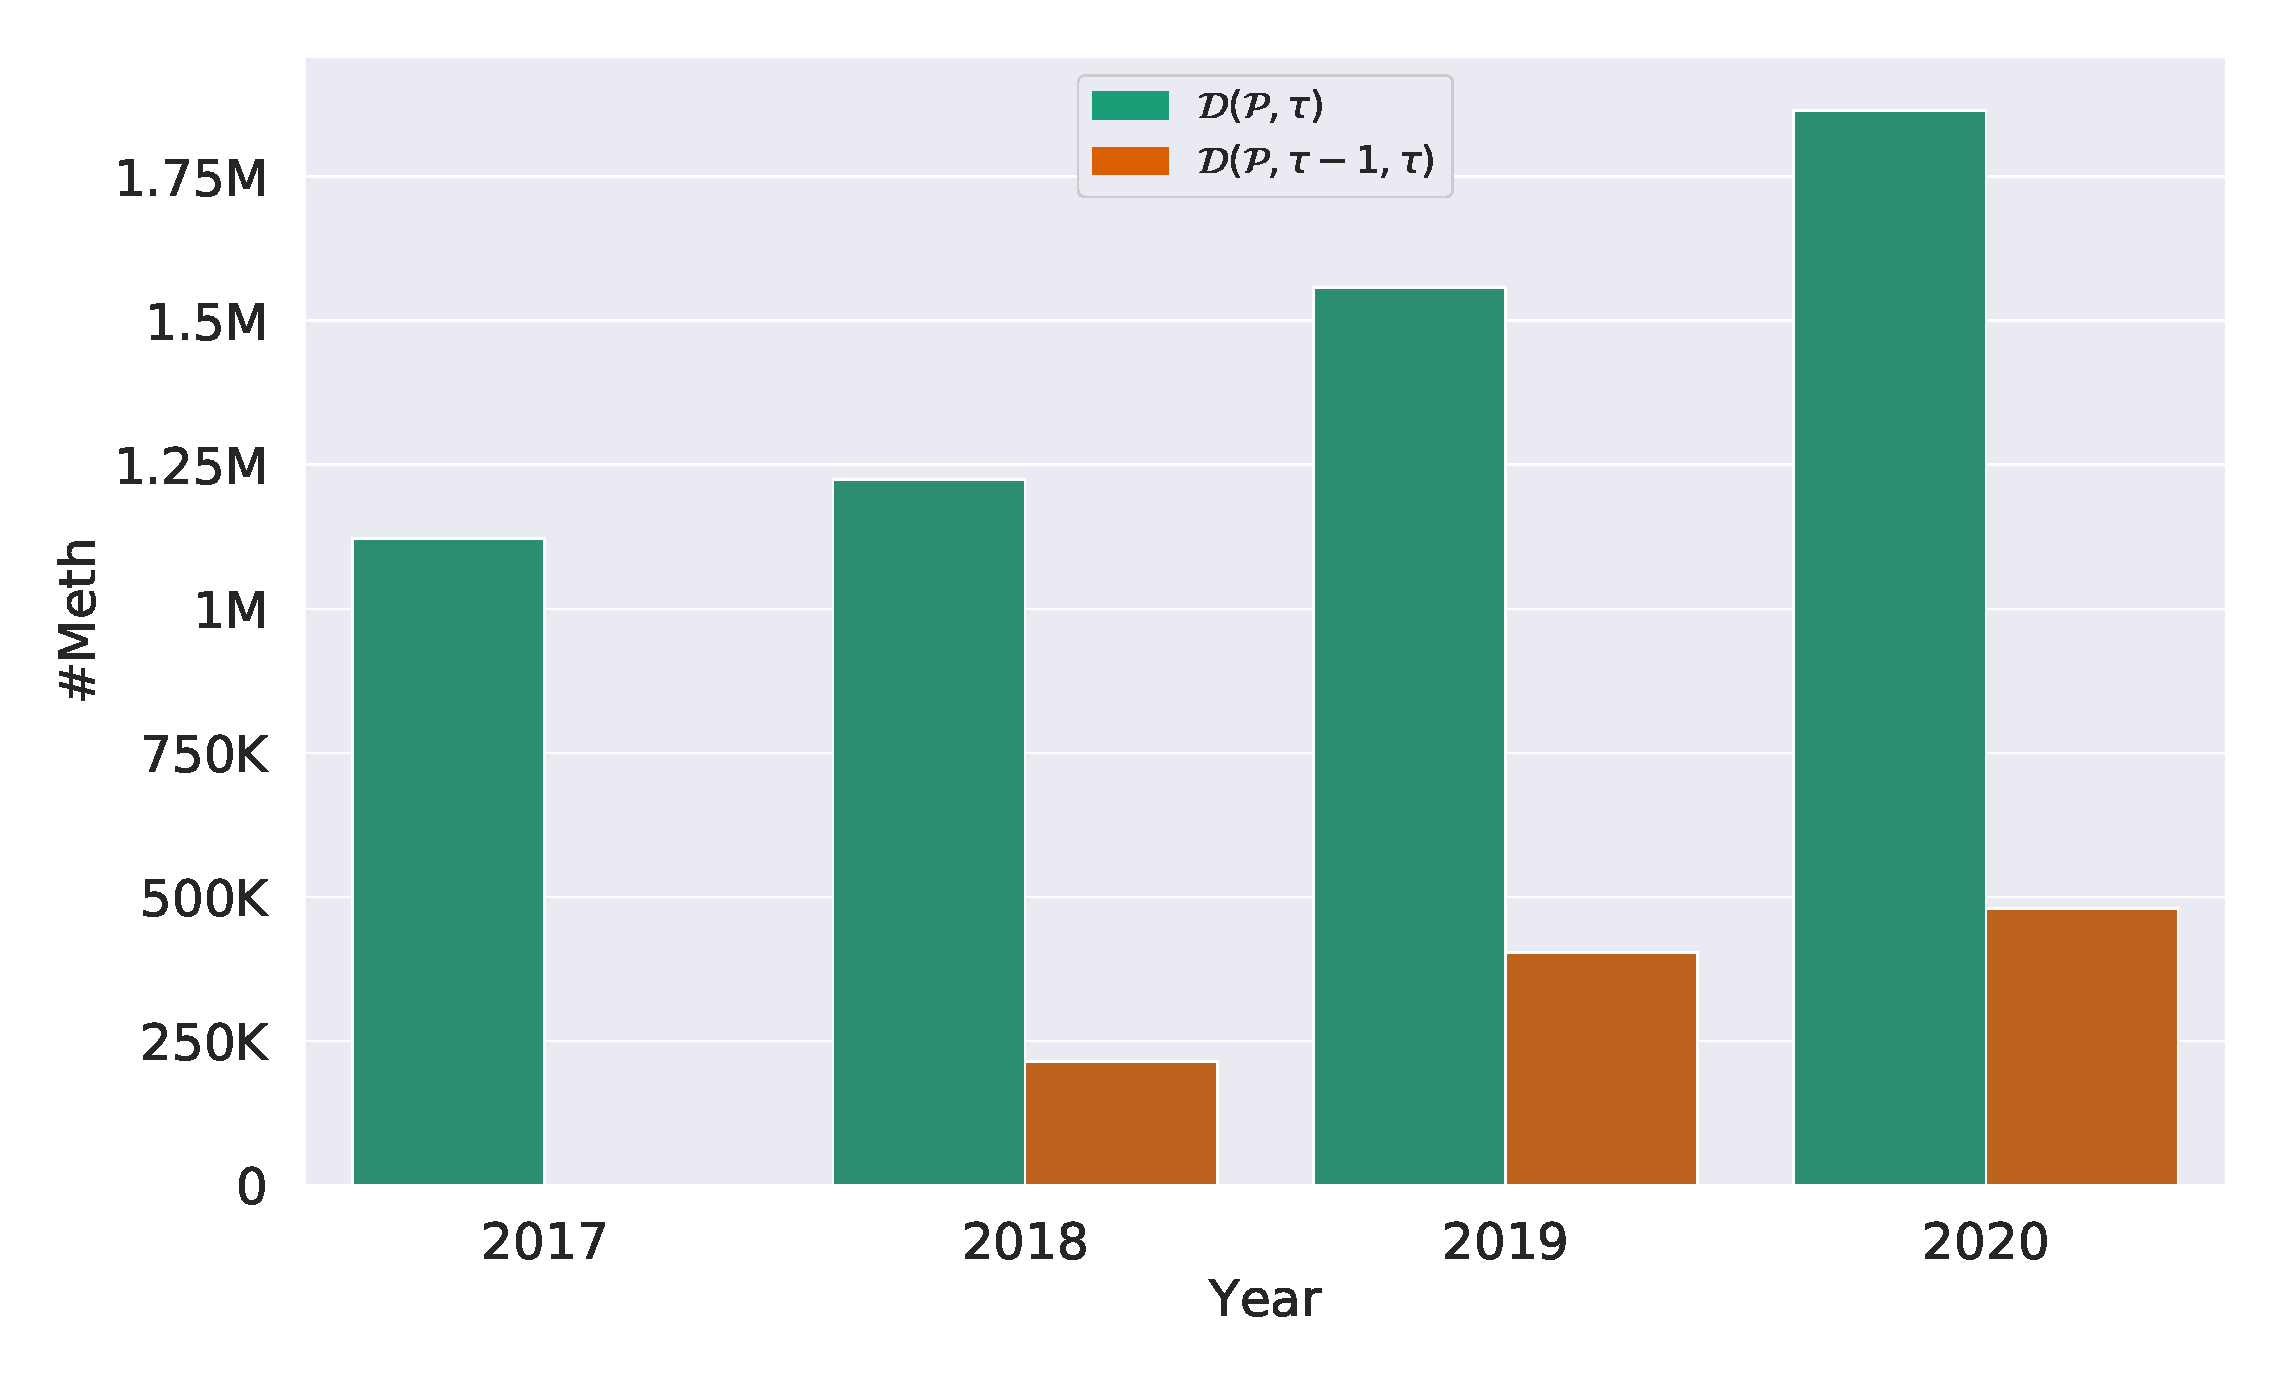
\includegraphics[width=.9\columnwidth]{figs/num-data-evolution.eps}
  \caption{Number of methods on each revision and new to each revision. \label{fig:num-data-evolution}}
\end{figure}

Figure~\ref{fig:num-data-evolution} shows the bar plots of the number
of methods on each revision of the \dataset, as well as the number of
methods new to each revision of the \dataset.  Figure~\ref{X} shows
the bar plots of the average length of methods, comments, and names on
each revision of the \dataset.

\section{Tasks}
\label{sec:tasks}

This section describes the two tasks in our study: \comgen and
\methnam.  For each task, we (1) give a brief summary of the
background, (2) select several recent well-studied machine learning
models to experiment with, and (3) describe the automatic metrics for
the task.

\subsection{\ComGen}
\label{sec:tasks:comgen}

\MyPara{Background} Developers frequently write comments in natural
language together with their code to deliver messages to their users
(e.g., via API comments) and to communicate among themselves (e.g.,
via todo
comments)~\cite{PadioleauETAL09Listening,NieETAL18Natural,PascarellaETAL19Classifying}.
Good comments help developers quickly and precisely comprehend code.
However, writing and maintaining comments can be tedious and
error-prone, making comments easy to be wrong or outdated, which leads
to inconsistencies and
bugs~\cite{TanETAL07Icomment,TanETAL12TComment,RatolAndRobillard17Detecting}.
The task of \comgen tries to automatically generate comments from
code.  So far, most related work~\cite{HuETAL18Deep,HuETAL19Deep,XXX}
focused on generating API comments (e.g., \javadoc summaries) from
methods.

\MyPara{Models} We select three models: \UseMacro{CG-Seq2seq},
\UseMacro{CG-Seq2seqAtt}, and \UseMacro{CG-DeepCom}.  All three models
formulate the \comgen task as a machine translation problem, and
exploits encoder-decoder neural networks to solve it.

\UseMacro{CG-Seq2seq} uses a vanilla encoder-decoder neural network,
where both the encoder and the decoder are single-layer GRU recurrent
neural network~\cite{ChoETAL14Learning}.  This model is usually used
as a baseline
%to compare against
in prior work based on deep learning. \Fix{You need to cite the prior work here}

\UseMacro{CG-Seq2seqAtt} is an upgraded version of
\UseMacro{CG-Seq2seq} that is altered with the attention mechanism
(specifically, the global attention model proposed in Luong et
al.~\cite{LuongETAL15Effective}).  The attention mechanism improves
the encoder-decoder neural network's ability in capturing long-range
dependencies among input tokens.

\UseMacro{CG-DeepCom}, recently proposed by Hu et
al.~\cite{HuETAL19Deep}, is a state-of-the-art deep learning model for
\comgen.  It exploits an encoder-decoder neural network that combines
both lexical and structural inputs: the code tokens and the AST
(abstract syntax tree) tokens, by using two encoders rather than one.
Figure~\ref{X} illustrates the architecture of this model.  The tree
structure in the AST is sequentialized by performing a novel
``structure-based'' traversal.  It also employs the attention
mechanism for both inputs.

\MyPara{Automated metrics} We use two automated metrics: average
sentence-level \bleu-4~\cite{XXX} and \xmatch. The \xmatch is the
percentage of examples for which the model's prediction is exactly the
same with reference comments.  \bleu is one of the most popular
language generation metrics which produces the score based on matches
of 4-grams of words between the reference and prediction.\Fix{maybe an example?}

%% # Comment generation
%% - Use cases: evolution, mixed-project, cross-project;
%% - Models: DeepCom-Hybrid, Seq2seq, Seq2seqAtt;
%% - 3 use cases * 3 models * 3 trials = 27 jobs to run

\subsection{\MethNam}
\label{sec:tasks:methnam}

\MyPara{Background} Descriptive and conventional names for code
elements (variables, methods, classes, etc.) are a vital part of
readable and maintainable code~\cite{XXX}.  Naming methods is
particularly hard and important, because the names need to be both
concise, usually containing only a few tokens and being much shorter
than the methods they are summarizing, and comprehensible, such that
they deliver the key functionality of the
code~\cite{LawrieETAL06Whats}.  Prior work explored various approaches
to solve the task, including information retrieval~\cite{XXX},
statistical~\cite{XXX}, and deep
learning~\cite{AllamanisETAL16Convolutional, XuETAL19Method,
  YonaiETAL19Mercem, AlonETAL19Code2vec, AlonETAL19code2seq,
  NguyenETAL20Suggesting}.

\MyPara{Models} We selected several recent deep learning based models
for this task:\UseMacro{MN-Bi-LSTM}, \UseMacro{MN-no-split-Bi-LSTM},
\UseMacro{MN-Code2Seq}.  They all formulate the task as a machine
translation problem from code to method names, and solve that using encoder-decoder neural
networks.

\UseMacro{MN-Bi-LSTM} uses bidirectional LSTM-based encoder-decoder
architecture with global attention. It takes method body as input and
outputs the target method names tokens while decoding.

\UseMacro{MN-no-split-Bi-LSTM} shares the same architecture as
\UseMacro{MN-Bi-LSTM} except that the tokens in the input method body
and target sequences are not split into subtokens.

\Fix{Any prior work you need to cite for the above two methods?}

\UseMacro{MN-Code2Seq}, proposed by Alon et
al.~\cite{AlonETAL19code2seq}, leverages the syntactic structure of
programming languages by extracting paths in abstract syntax tree
(AST) to represent a code snippet.Each path is encoded into a
fixed-length vector using LSTMs. Global attention is applied to all
the paths during decoding to generate the target method names.

\MyPara{Automated metrics} In addition to \xmatch, we adopt the
automated metrics: \fone, \precision, \recall used by Allamanis et
al.~\cite{AllamanisETAL16Convolutional} and Alon et
al. ~\cite{AlonETAL19code2seq} to measure models' performance.

%% # Method name generation
%% - Use cases: evolution, mixed-project, cross-project;
%% - Models: Code2Seq, BiLSTM, BiLSTM(no-split);
%%   // Ideally add Transformer, in which case BiLSTM(no-split) can be removed
%% - 3 use cases * 3 models * 3 trials = 27 jobs to run




%% ---------- below are OLD design before Aug 22, 2020 ----------

%% We define \textit{evolution-aware} evaluation setting as following.
%% %
%% We take $k$ snapshots of a evolving \dataset $\{S_1, S_2, \dots,
%% S_k\}$ at time points $\{t_1, t_2, \dots, t_k\}$ respectively in
%% chronological order.
%% %
%% To evaluate a ML technique on $S_{i+1}$, we only train the technique
%% on the data available before $t_{i+1}$, i.e., $\{S_1, \dots, S_i\}$.
%% %
%% We define task-specific filter functions $F_j(S_{i+1}, S_i)$ to obtain
%% subsets of $S_{i+1}$ for evaluation in different settings; for
%% example, removing data points that already existed in $S_i$ to perform
%% an ``unbiased'' (in ML view) evaluation.

%% Given the project data available at $k$ different time points $\{t_1,
%% \dots, t_k\}$, at each time point $t_i$, we train our system on
%% all the data available at time $t_i$ then test on the data existing at
%% time $t_{i+1}$ which are filtered by the task specific filter function
%% $F$.

%% In contrast, we define \textit{evolution-unaware} evaluation setting
%% as randomly separating the data points in $S_k$ into three subsets:
%% $S_{train}$, $S_{val}$, $S_{test}$.  Then, we train the technique on
%% $S_{train}$ with $F(S_{val}, S_{train})$ as validation set, and
%% evaluate the trained technique on $F(S_{test}, S_{train} \sunion
%% S_{val}$.

%% Our goal is to evaluate the same set of machine learning techniques
%% using both evolution-aware setting and evolution-unaware setting to
%% testify whether the observations made in evolution-unaware setting are
%% still valid in evolution-aware setting.

%% \subsection{Comment Generation}

%% \subsubsection{Filter Functions}

%% We evaluate in three settings using three different filter functions.

%% $F_a$ will remove all the methods in $S_{i+1}$ that have same
%% signature with some methods in $S_i$. Here, signature is the tuple of
%% (class name [including outer class name if in an inner class], method
%% name, argument types).  Since most comment generation models only take
%% method snippets (method name, return type, arguments and method body)
%% as input, the filter function ensures the methods in $S_{i+1}$ have
%% not been seen by the model during training.  This also ensures moving
%% files between packages do not result in ``new'' methods.

%% $F_b$ will filter all the methods that have same signature and same
%% method body with some methods in $S_i$, i.e., include the new methods
%% and methods that have been updated between two time points.

%% $F_c$ will filter all the methods in time $S_{i+1}$ that have same
%% signature, same method body and same fully-qualified class name with
%% some methods in $S_i$ to avoid data leakage, i.e., include new
%% methods, updated methods and the methods that are simply copied or
%% moved from one file to another.

%% We denote the subsets after filtering as:

%% \begin{flalign*}
%%   S^a_{i+1} &= F_a(S_{i+1}, S_i) \\
%%   S^b_{i+1} &= F_b(S_{i+1}, S_i) \\
%%   S^c_{i+1} &= F_c(S_{i+1}, S_i)
%% \end{flalign*}

%% Note that $S^a_{i+1} \subseteq S^b_{i+1} \subseteq
%% S^c_{i+1} \subseteq S_{i+1}$.


%% \subsubsection{Data}

%% We collected the \dataset of comment-code pairs from the same
%% repositories in \citet{HuETAL18Deep}.
%% We take the snapshots of the \dataset at these time points:

%% \begin{flalign*}
%%   t_1 = \text{Jan 1 2013}&,\quad t_2 = \text{Jan 1 2014}, \\
%%   t_3 = \text{Jan 1 2015}&,\quad t_4 = \text{Jan 1 2016}, \\
%%   t_5 = \text{Jan 1 2017}&,\quad t_6 = \text{Jan 1 2018}, \\
%%   t_7 = \text{Jan 1 2019}&,\quad t_8 = \text{Jan 1 2020}
%% \end{flalign*}

%% We consider the type of experiment of training the technique on the
%% first year's data with the second year's data as validation set, and
%% testing on the third year's data.  This setting assumes that new
%% comments should follow similar style of recently-written comments.  We
%% perform 5 groups of experiments:

%% \begin{enumerate}
%% \item Train on $S^a_2$ with $S^a_3$ as validation set, and
%%   test on $S^{a,b,c}_4$.
%% \item Train on $S^a_3$ with $S^a_4$ as validation set, and
%%   test on $S^{a,b,c}_5$.
%% \item Train on $S^a_4$ with $S^a_5$ as validation set, and
%%   test on $S^{a,b,c}_6$.
%% \item Train on $S^a_5$ with $S^a_6$ as validation set, and
%%   test on $S^{a,b,c}_7$.
%% \item Train on $S^a_6$ with $S^a_7$ as validation set, and
%%   test on $S^{a,b,c}_8$.
%% \end{enumerate}

%% An alternative type of experiment would be training on all data before
%% a time point with the next year's data as validation set, and testing
%% on the following next year's data.  For example, train on $S_1$ with
%% $S^a_2$ as validation set, and test on $S^a_3$.  However, in
%% this setting, obsolete comments may dominate the training set and thus
%% bias the predictions of techniques.

%% Different from DeepCom's data processing procedure, we do not
%% filtering getter, setter, or constructor methods, where our main
%% consideration is to focus on the comparison of different evaluation
%% setting and avoid any bias that might be introduced by this additional
%% step.

%% \subsubsection{Techniques}

%% Hybrid-DeepCom, DeepCom(SBT), DeepCom(Pre-order), Seq2Seq(Attention), Seq2Seq.


%% \subsection{Method Name Generation}

%% \subsubsection{Filtering Functions}
%% $F_a$ will remove all the methods in $S_{i+1}$ that have same
%% method name, class name [including outer class name if in an inner
%%   class] and method body with some methods in $S_i$.
%% \subsubsection{Data}

%% \subsubsection{Techniques}

%% Code2seq, 2-layer BiLSTM(no token splitting), 2-layer BiLSTM,
%% potentially code2vec.

\section{Results and Findings}
\label{sec:eval}

This section describes our experiment results and findings.  We (1)
describe the training details of our experiment, including the
environment and hyper-parameters, (2) show the results for \comgen and
\methnam tasks, and (3) list the key observations and findings from
our experiment.

\subsection{Training Details}
\label{sec:eval:hyparam}

We trained and tested all models on a super computer, where each model
use a NVIDIA GTX 1080-TI GPU and four models share two Intel(R)
Xeon(R) CPU E5-2620 CPUs and 128GB of RAM.  We trained and tested each
model in each evaluation setting \NumTrial times and each run is
initialized using different random seed.

We followed the source literature to setup the hyper-parameters of
models. \Fix{...}

\subsection{Results for \ComGen}
\label{sec:eval:results-comgen}


%% Automatically generated by pyutil.latex 

\begin{table*}
\begin{small}
\begin{center}
\caption{\TCResultsComGen}
\begin{tabular}{l|rr|rr|rr}
\toprule
 & \multicolumn{2}{c|}{\UseMacro{TH-exp-mixedproj-2020}}
 & \multicolumn{2}{c|}{\UseMacro{TH-exp-crossproj-2020}}
 & \multicolumn{2}{c}{\UseMacro{TH-exp-evo-2020}}
\\
\multirow{-2}{*}{\THModel} 
 & \UseMacro{TH-metric-bleu}
 & \UseMacro{TH-metric-xmatch}
 & \UseMacro{TH-metric-bleu}
 & \UseMacro{TH-metric-xmatch}
 & \UseMacro{TH-metric-bleu}
 & \UseMacro{TH-metric-xmatch}
\\
\midrule
\UseMacro{TH-model-Seq2seq}
 & \UseMacro{mixedproj-2020-test_common-bleu-Seq2seq-AVG}
 & \UseMacro{mixedproj-2020-test_common-xmatch-Seq2seq-AVG}$^{\gamma\epsilon}$
 & \UseMacro{crossproj-2020-test_common-bleu-Seq2seq-AVG}
 & \UseMacro{crossproj-2020-test_common-xmatch-Seq2seq-AVG}
 & \UseMacro{evo-2020-test_common-bleu-Seq2seq-AVG}
 & \UseMacro{evo-2020-test_common-xmatch-Seq2seq-AVG}$^{\zeta\theta}$
\\
\UseMacro{TH-model-Seq2seqAtt}
 & \UseMacro{mixedproj-2020-test_common-bleu-Seq2seqAtt-AVG}$^{\alpha}$
 & \UseMacro{mixedproj-2020-test_common-xmatch-Seq2seqAtt-AVG}$^{\delta\epsilon}$
 & \UseMacro{crossproj-2020-test_common-bleu-Seq2seqAtt-AVG}
 & \UseMacro{crossproj-2020-test_common-xmatch-Seq2seqAtt-AVG}
 & \UseMacro{evo-2020-test_common-bleu-Seq2seqAtt-AVG}$^{\beta}$
 & \UseMacro{evo-2020-test_common-xmatch-Seq2seqAtt-AVG}$^{\eta\theta}$
\\
\UseMacro{TH-model-DeepCom}
 & \UseMacro{mixedproj-2020-test_common-bleu-DeepCom-AVG}$^{\alpha}$
 & \UseMacro{mixedproj-2020-test_common-xmatch-DeepCom-AVG}$^{\gamma\delta}$
 & \UseMacro{crossproj-2020-test_common-bleu-DeepCom-AVG}
 & \UseMacro{crossproj-2020-test_common-xmatch-DeepCom-AVG}
 & \UseMacro{evo-2020-test_common-bleu-DeepCom-AVG}$^{\beta}$
 & \UseMacro{evo-2020-test_common-xmatch-DeepCom-AVG}$^{\zeta\eta}$
\\
\bottomrule
\end{tabular}
\end{center}
\end{small}
\vspace{\TVResultsComGen}
\end{table*}


Table~\ref{table:results-com-gen} shows the automatic metrics (\bleu
and \xmatch) for each \methodology (\mixedproj, \crossproj, and
\evoaware) for the models we selected for the \comgen task.

\begin{figure}[t]
  \centering
  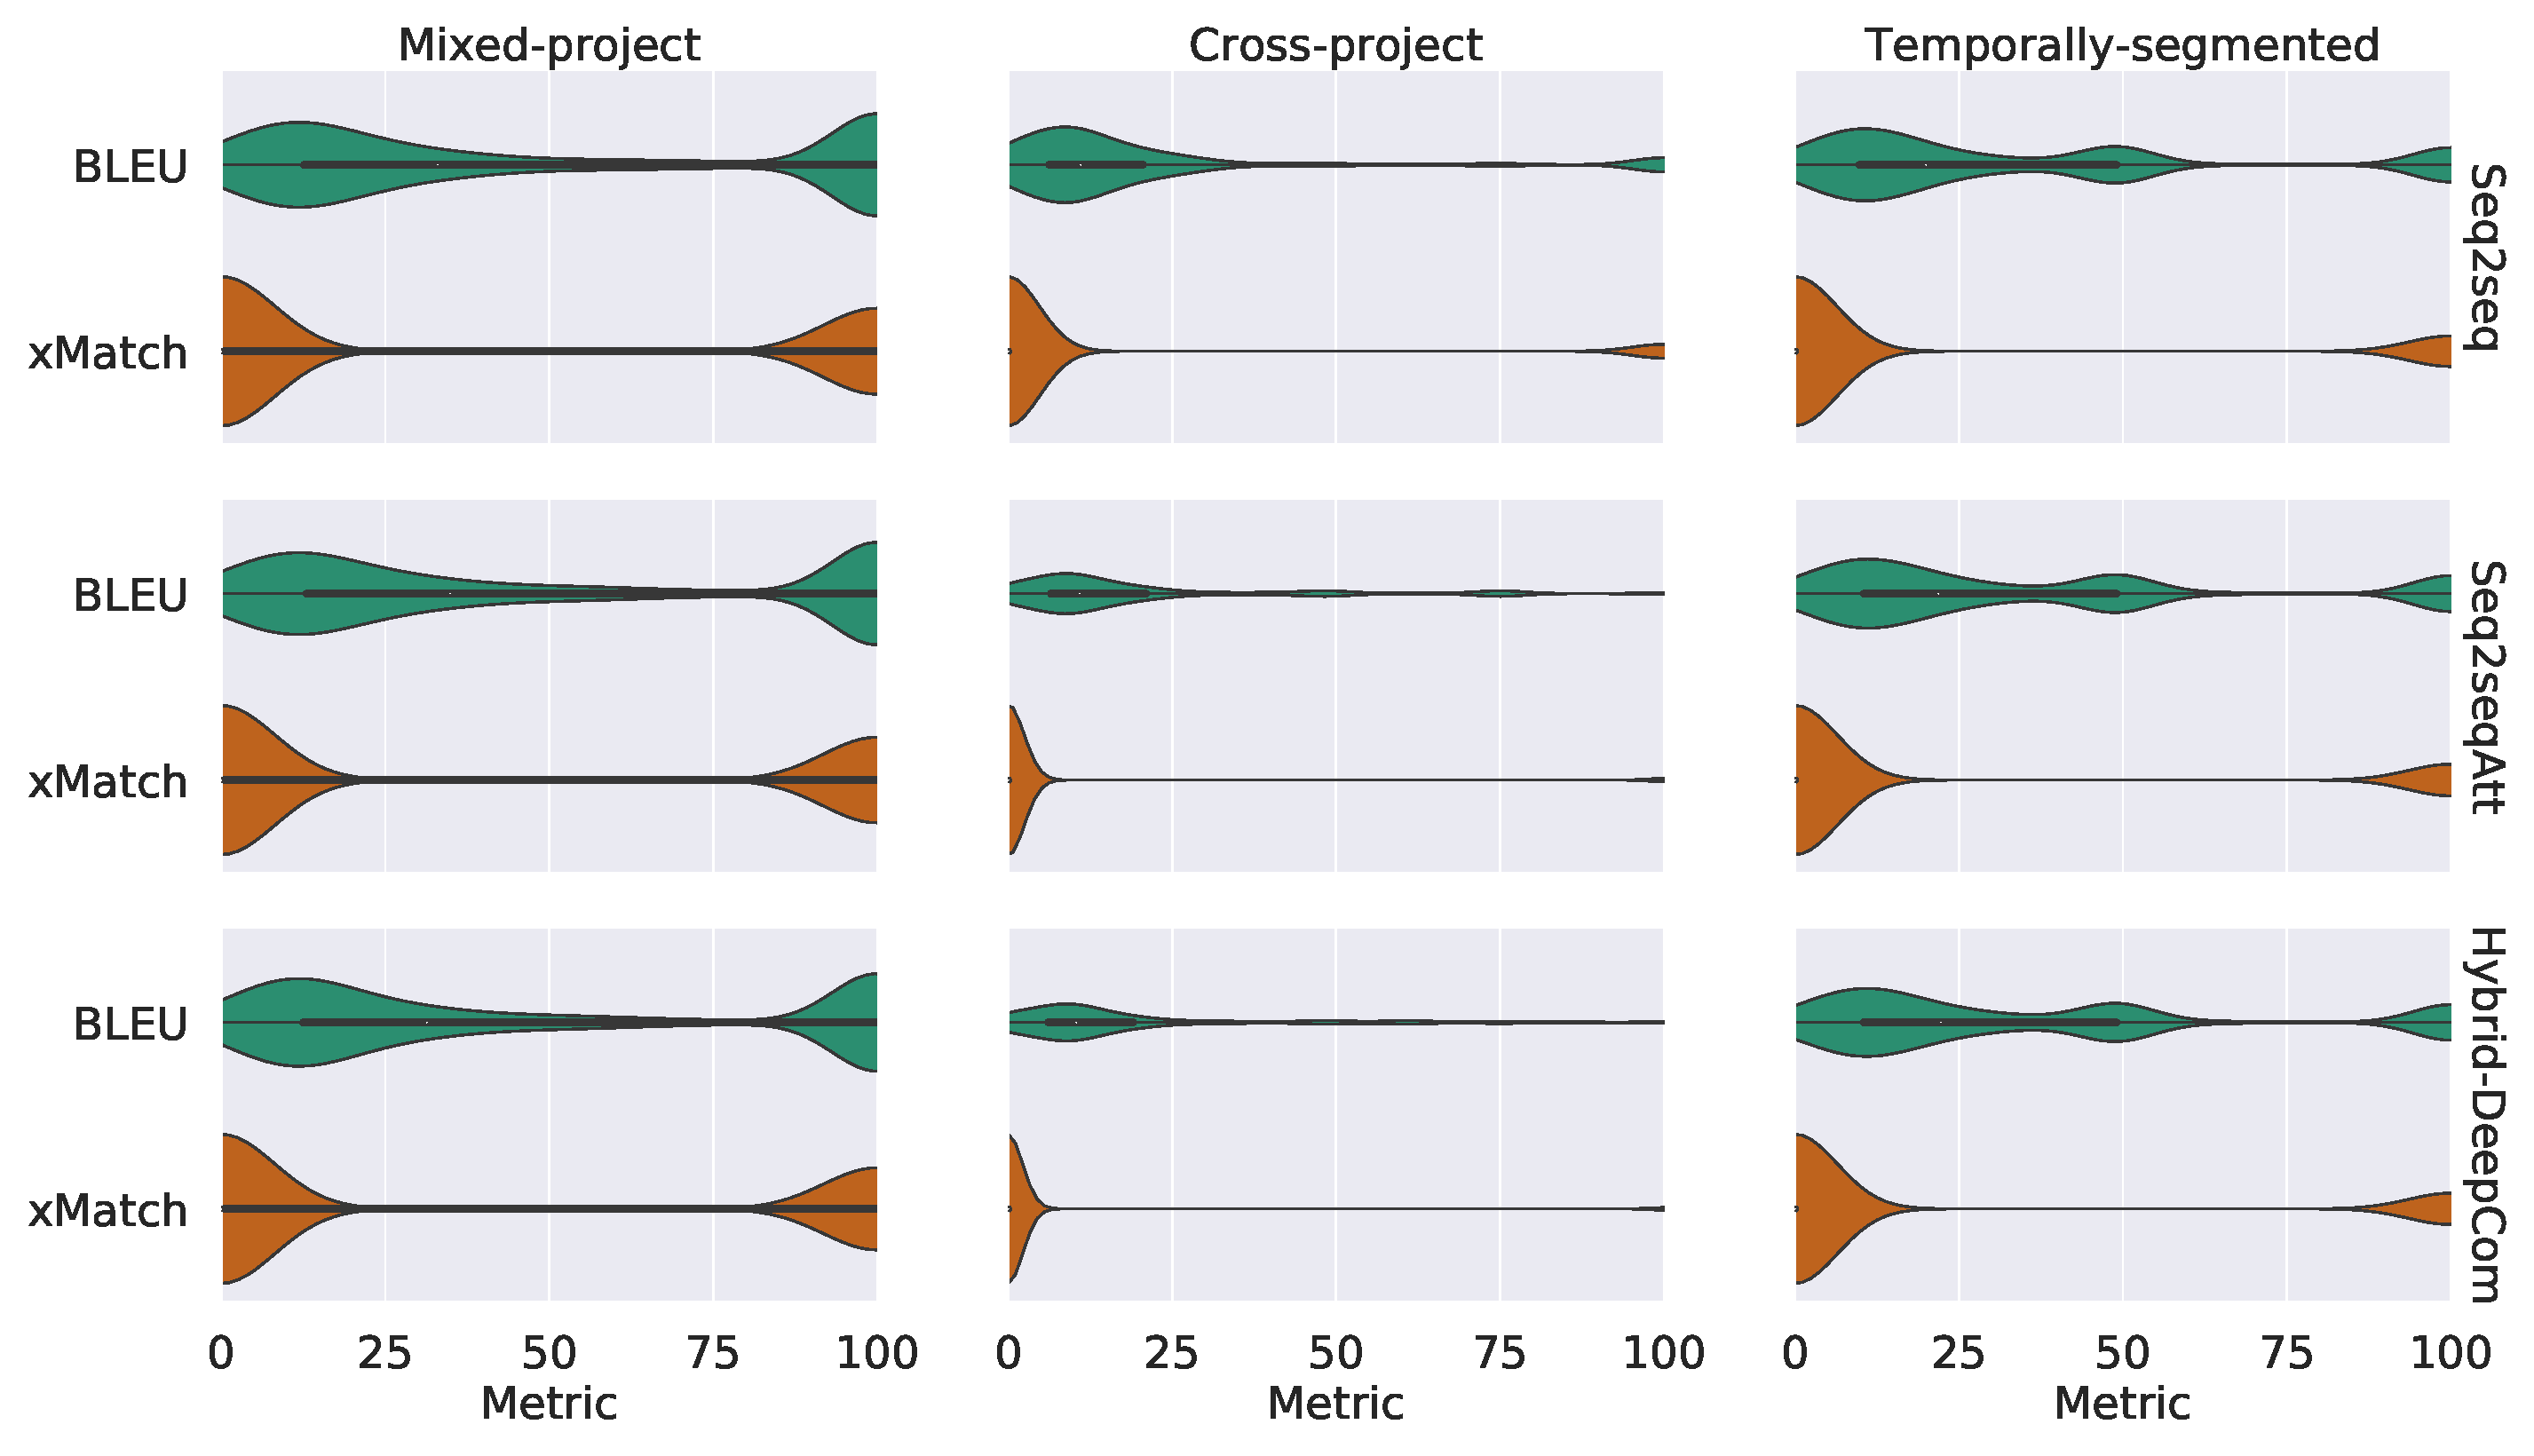
\includegraphics[width=\columnwidth]{figs/models-results-metrics-dist-ComGen.eps}
  \caption{Each violin plot shows the distribution of automated
    metrics on all examples in \test set.  Left to right: \mixedproj,
    \crossproj, and \evoaware \methodologies.  Top to bottom: the
    models for \comgen
    task. \label{fig:models-results-metrics-dist-ComGen}}
\end{figure}

\begin{figure}[t]
  \centering
  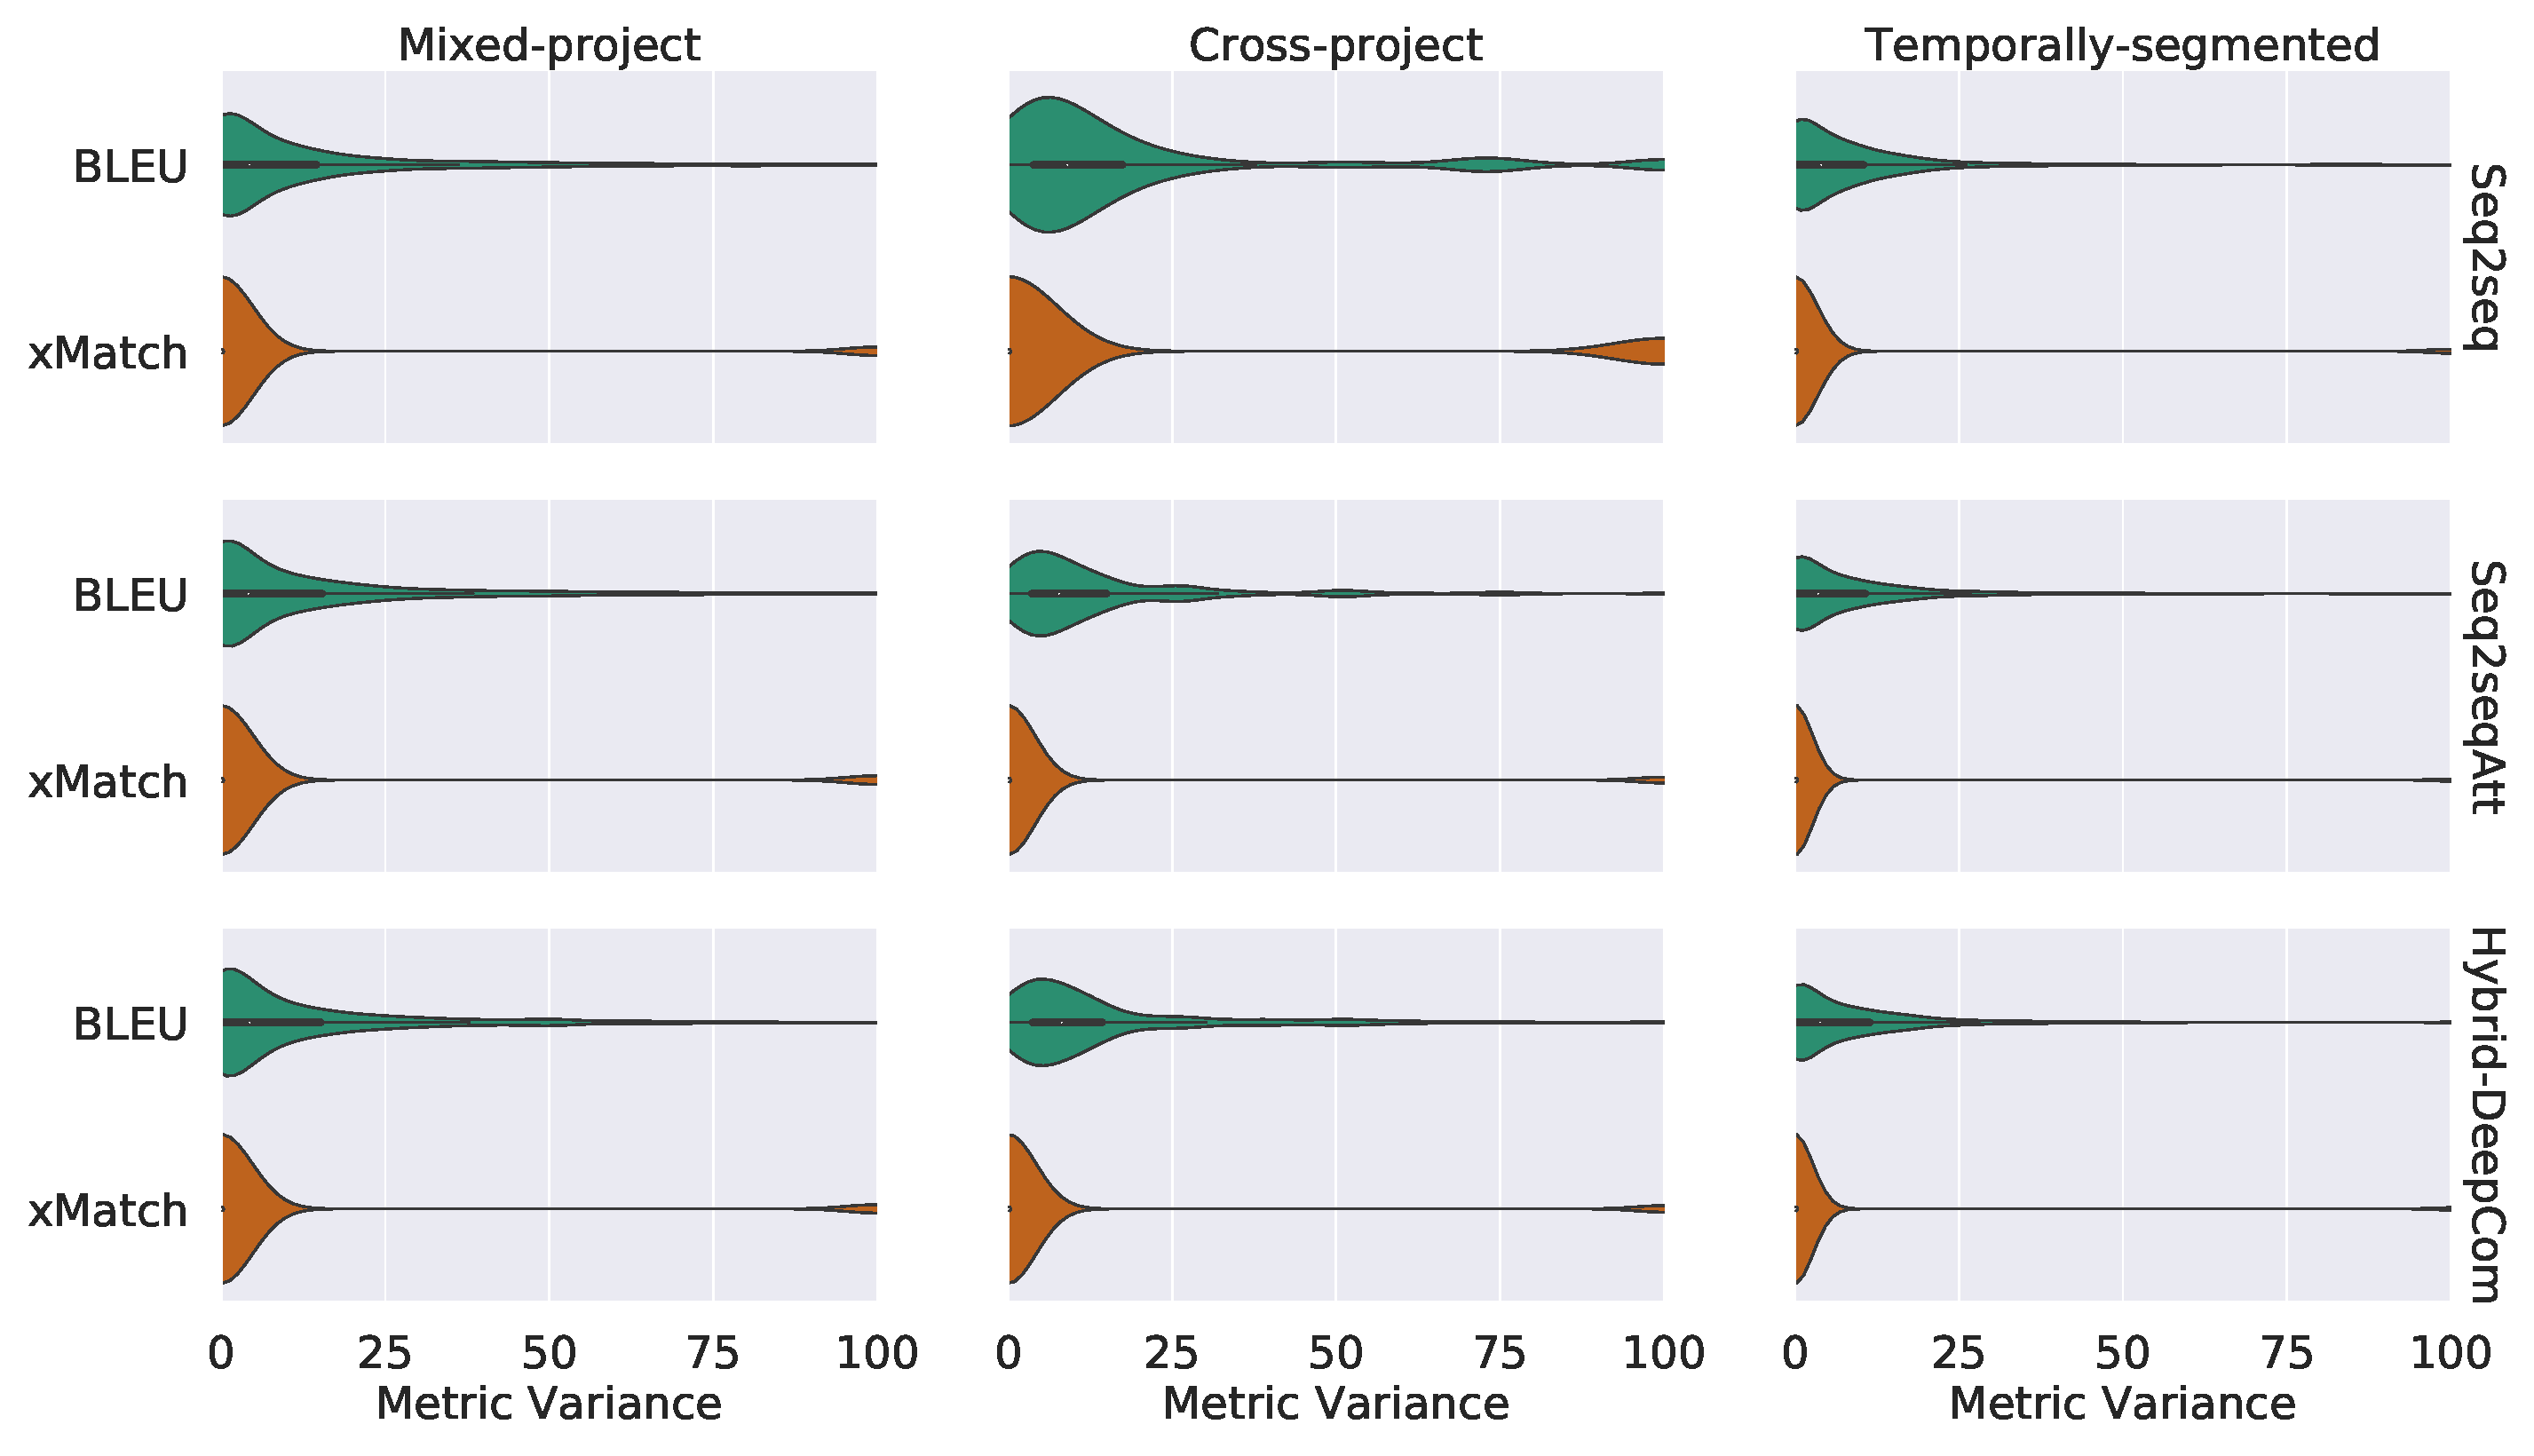
\includegraphics[width=\columnwidth]{figs/models-results-variance-dist-ComGen.eps}
  \caption{Each violin plot shows the distribution of the variances of
    automated metrics on all examples in \test set between \NumTrial
    trials.  Left to right: \mixedproj, \crossproj, and \evoaware
    \methodologies.  Top to bottom: the models for \comgen
    task. \label{fig:models-results-variance-dist-ComGen}}
\end{figure}

Figure~\ref{fig:models-results-metrics-dist-ComGen} shows the
distributions of automatic metrics on examples in \test set.
Figure~\ref{fig:models-results-variance-dist-ComGen} shows the
distributions of the variances of automated metrics on examples in
\test between \NumTrial different trials, where the variance is
calculated as the diff of the maximum value in \NumTrial trials and
minimum value in \NumTrial trials.


\subsection{Results for \MethNam}
\label{sec:eval:results-methnam}


%% Automatically generated by pyutil.latex 

\begin{table*}
\begin{small}
\begin{center}
\caption{\TCResultsMethNam}
\begin{tabular}{l|rrrr|rrrr|rrrr}
\toprule
 & \multicolumn{4}{c|}{\UseMacro{TH-exp-mixedproj-2020}}
 & \multicolumn{4}{c|}{\UseMacro{TH-exp-crossproj-2020}}
 & \multicolumn{4}{c}{\UseMacro{TH-exp-evo-2020}}
\\
\multirow{-2}{*}{\THModel} 
 & \UseMacro{TH-metric-f1}
 & \UseMacro{TH-metric-precision}
 & \UseMacro{TH-metric-recall}
 & \UseMacro{TH-metric-xmatch}
 & \UseMacro{TH-metric-f1}
 & \UseMacro{TH-metric-precision}
 & \UseMacro{TH-metric-recall}
 & \UseMacro{TH-metric-xmatch}
 & \UseMacro{TH-metric-f1}
 & \UseMacro{TH-metric-precision}
 & \UseMacro{TH-metric-recall}
 & \UseMacro{TH-metric-xmatch}
\\
\midrule
\UseMacro{TH-model-Bi-LSTM}
 & \UseMacro{mixedproj-2020-test_common-f1-Bi-LSTM-AVG}$^{\alpha}$
 & \UseMacro{mixedproj-2020-test_common-precision-Bi-LSTM-AVG}$^{\delta}$
 & \textbf{\UseMacro{mixedproj-2020-test_common-recall-Bi-LSTM-AVG}}$^{\eta}$
 & \UseMacro{mixedproj-2020-test_common-xmatch-Bi-LSTM-AVG}$^{\kappa}$
 & \textbf{\UseMacro{crossproj-2020-test_common-f1-Bi-LSTM-AVG}}$^{\beta}$
 & \textbf{\UseMacro{crossproj-2020-test_common-precision-Bi-LSTM-AVG}}$^{\epsilon}$
 & \textbf{\UseMacro{crossproj-2020-test_common-recall-Bi-LSTM-AVG}}$^{\theta}$
 & \textbf{\UseMacro{crossproj-2020-test_common-xmatch-Bi-LSTM-AVG}}$^{\lambda}$
 & \textbf{\UseMacro{evo-2020-test_common-f1-Bi-LSTM-AVG}}$^{\gamma}$
 & \textbf{\UseMacro{evo-2020-test_common-precision-Bi-LSTM-AVG}}$^{\zeta}$
 & \textbf{\UseMacro{evo-2020-test_common-recall-Bi-LSTM-AVG}}$^{\iota}$
 & \UseMacro{evo-2020-test_common-xmatch-Bi-LSTM-AVG}$^{\mu}$
\\
\UseMacro{TH-model-no-split-Bi-LSTM}
 & \textbf{\UseMacro{mixedproj-2020-test_common-f1-no-split-Bi-LSTM-AVG}}$^{\alpha}$
 & \textbf{\UseMacro{mixedproj-2020-test_common-precision-no-split-Bi-LSTM-AVG}}$^{\delta}$
 & \UseMacro{mixedproj-2020-test_common-recall-no-split-Bi-LSTM-AVG}$^{\eta}$
 & \textbf{\UseMacro{mixedproj-2020-test_common-xmatch-no-split-Bi-LSTM-AVG}}$^{\kappa}$
 & \UseMacro{crossproj-2020-test_common-f1-no-split-Bi-LSTM-AVG}$^{\beta}$
 & \UseMacro{crossproj-2020-test_common-precision-no-split-Bi-LSTM-AVG}$^{\epsilon}$
 & \UseMacro{crossproj-2020-test_common-recall-no-split-Bi-LSTM-AVG}$^{\theta}$
 & \UseMacro{crossproj-2020-test_common-xmatch-no-split-Bi-LSTM-AVG}$^{\lambda}$
 & \UseMacro{evo-2020-test_common-f1-no-split-Bi-LSTM-AVG}$^{\gamma}$
 & \UseMacro{evo-2020-test_common-precision-no-split-Bi-LSTM-AVG}$^{\zeta}$
 & \UseMacro{evo-2020-test_common-recall-no-split-Bi-LSTM-AVG}$^{\iota}$
 & \textbf{\UseMacro{evo-2020-test_common-xmatch-no-split-Bi-LSTM-AVG}}$^{\mu}$
\\
\UseMacro{TH-model-Code2Seq}
 & \UseMacro{mixedproj-2020-test_common-f1-Code2Seq-AVG}
 & \UseMacro{mixedproj-2020-test_common-precision-Code2Seq-AVG}
 & \UseMacro{mixedproj-2020-test_common-recall-Code2Seq-AVG}
 & \UseMacro{mixedproj-2020-test_common-xmatch-Code2Seq-AVG}
 & \UseMacro{crossproj-2020-test_common-f1-Code2Seq-AVG}
 & \UseMacro{crossproj-2020-test_common-precision-Code2Seq-AVG}
 & \UseMacro{crossproj-2020-test_common-recall-Code2Seq-AVG}
 & \UseMacro{crossproj-2020-test_common-xmatch-Code2Seq-AVG}
 & \UseMacro{evo-2020-test_common-f1-Code2Seq-AVG}
 & \UseMacro{evo-2020-test_common-precision-Code2Seq-AVG}
 & \UseMacro{evo-2020-test_common-recall-Code2Seq-AVG}
 & \UseMacro{evo-2020-test_common-xmatch-Code2Seq-AVG}
\\
\bottomrule
\end{tabular}
\end{center}
\end{small}
\vspace{\TVResultsMethNam}
\end{table*}


Table~\ref{table:results-meth-nam} shows the automatic metrics (\fone,
\precision, \recall, and \xmatch) for each \methodology (\mixedproj,
\crossproj, and \evoaware) for the models we selected for the \methnam
task.

\begin{figure}[t]
  \centering
  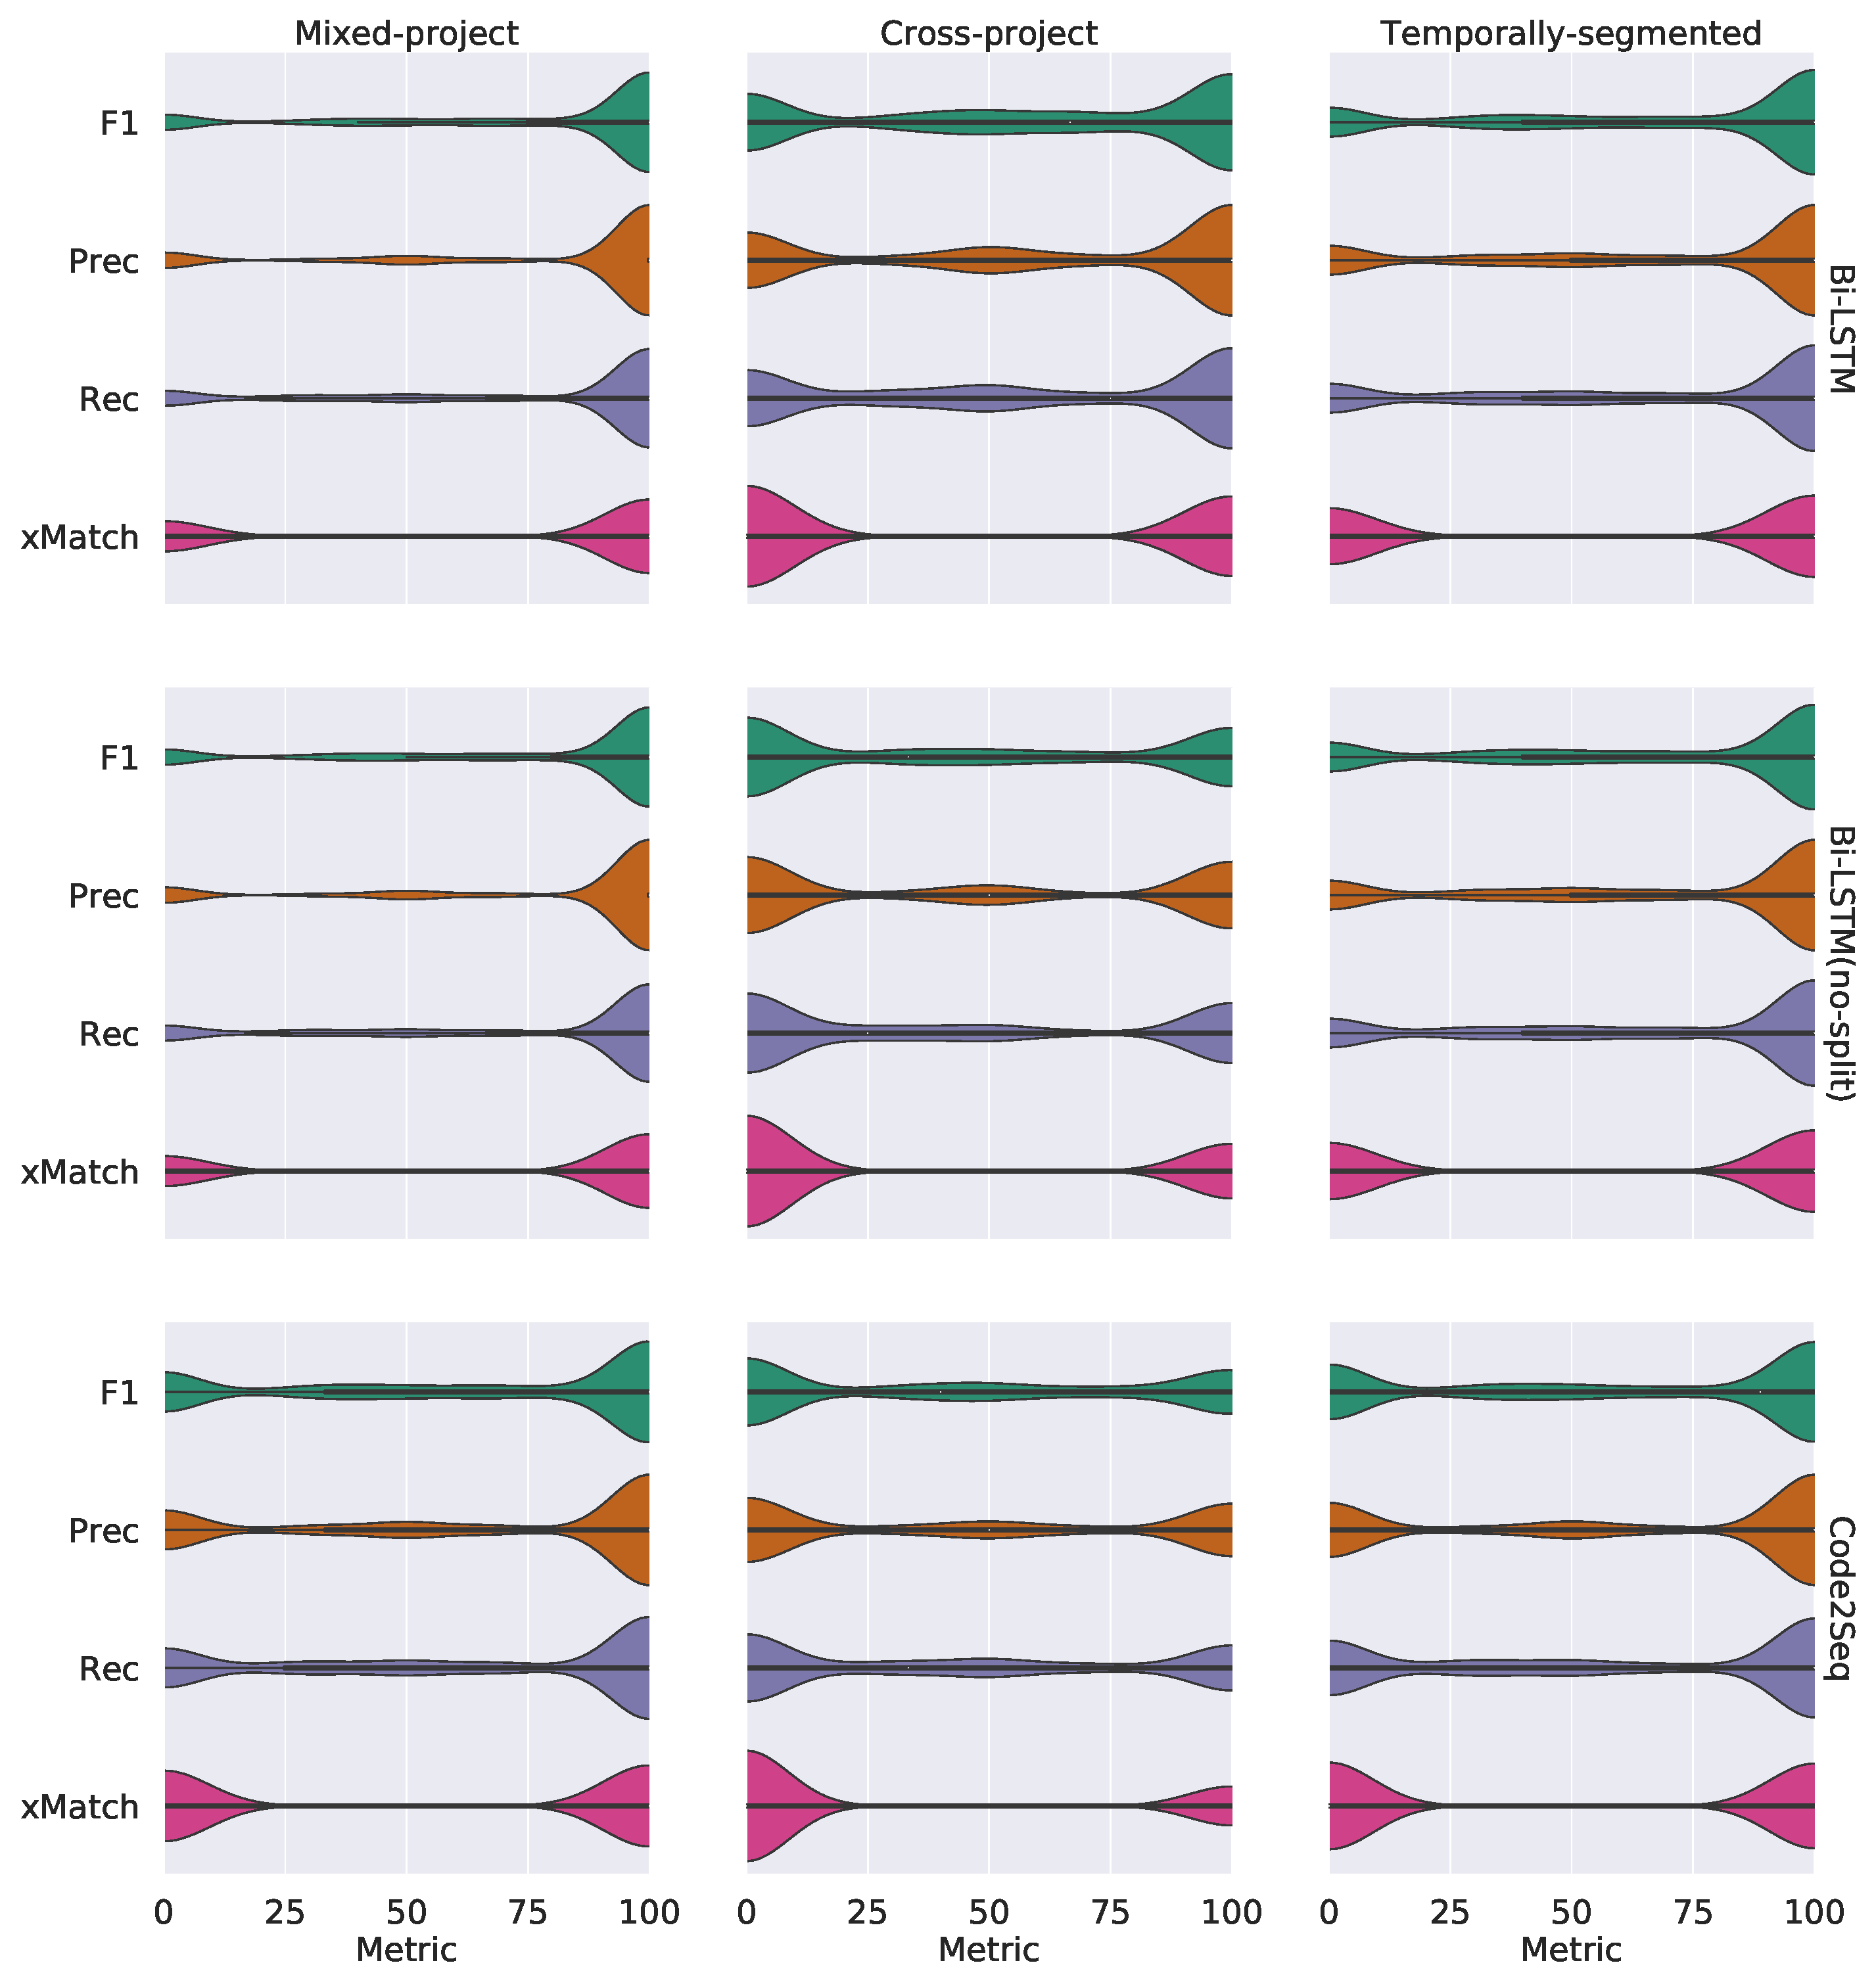
\includegraphics[width=\columnwidth]{figs/models-results-metrics-dist-MethNam.eps}
  \caption{Each violin plot shows the distribution of automated
    metrics on all examples in \test set.  Left to right: \mixedproj,
    \crossproj, and \evoaware \methodologies.  Top to bottom: the
    models for \methnam
    task. \label{fig:models-results-metrics-dist-MethNam}}
\end{figure}

\begin{figure}[t]
  \centering
  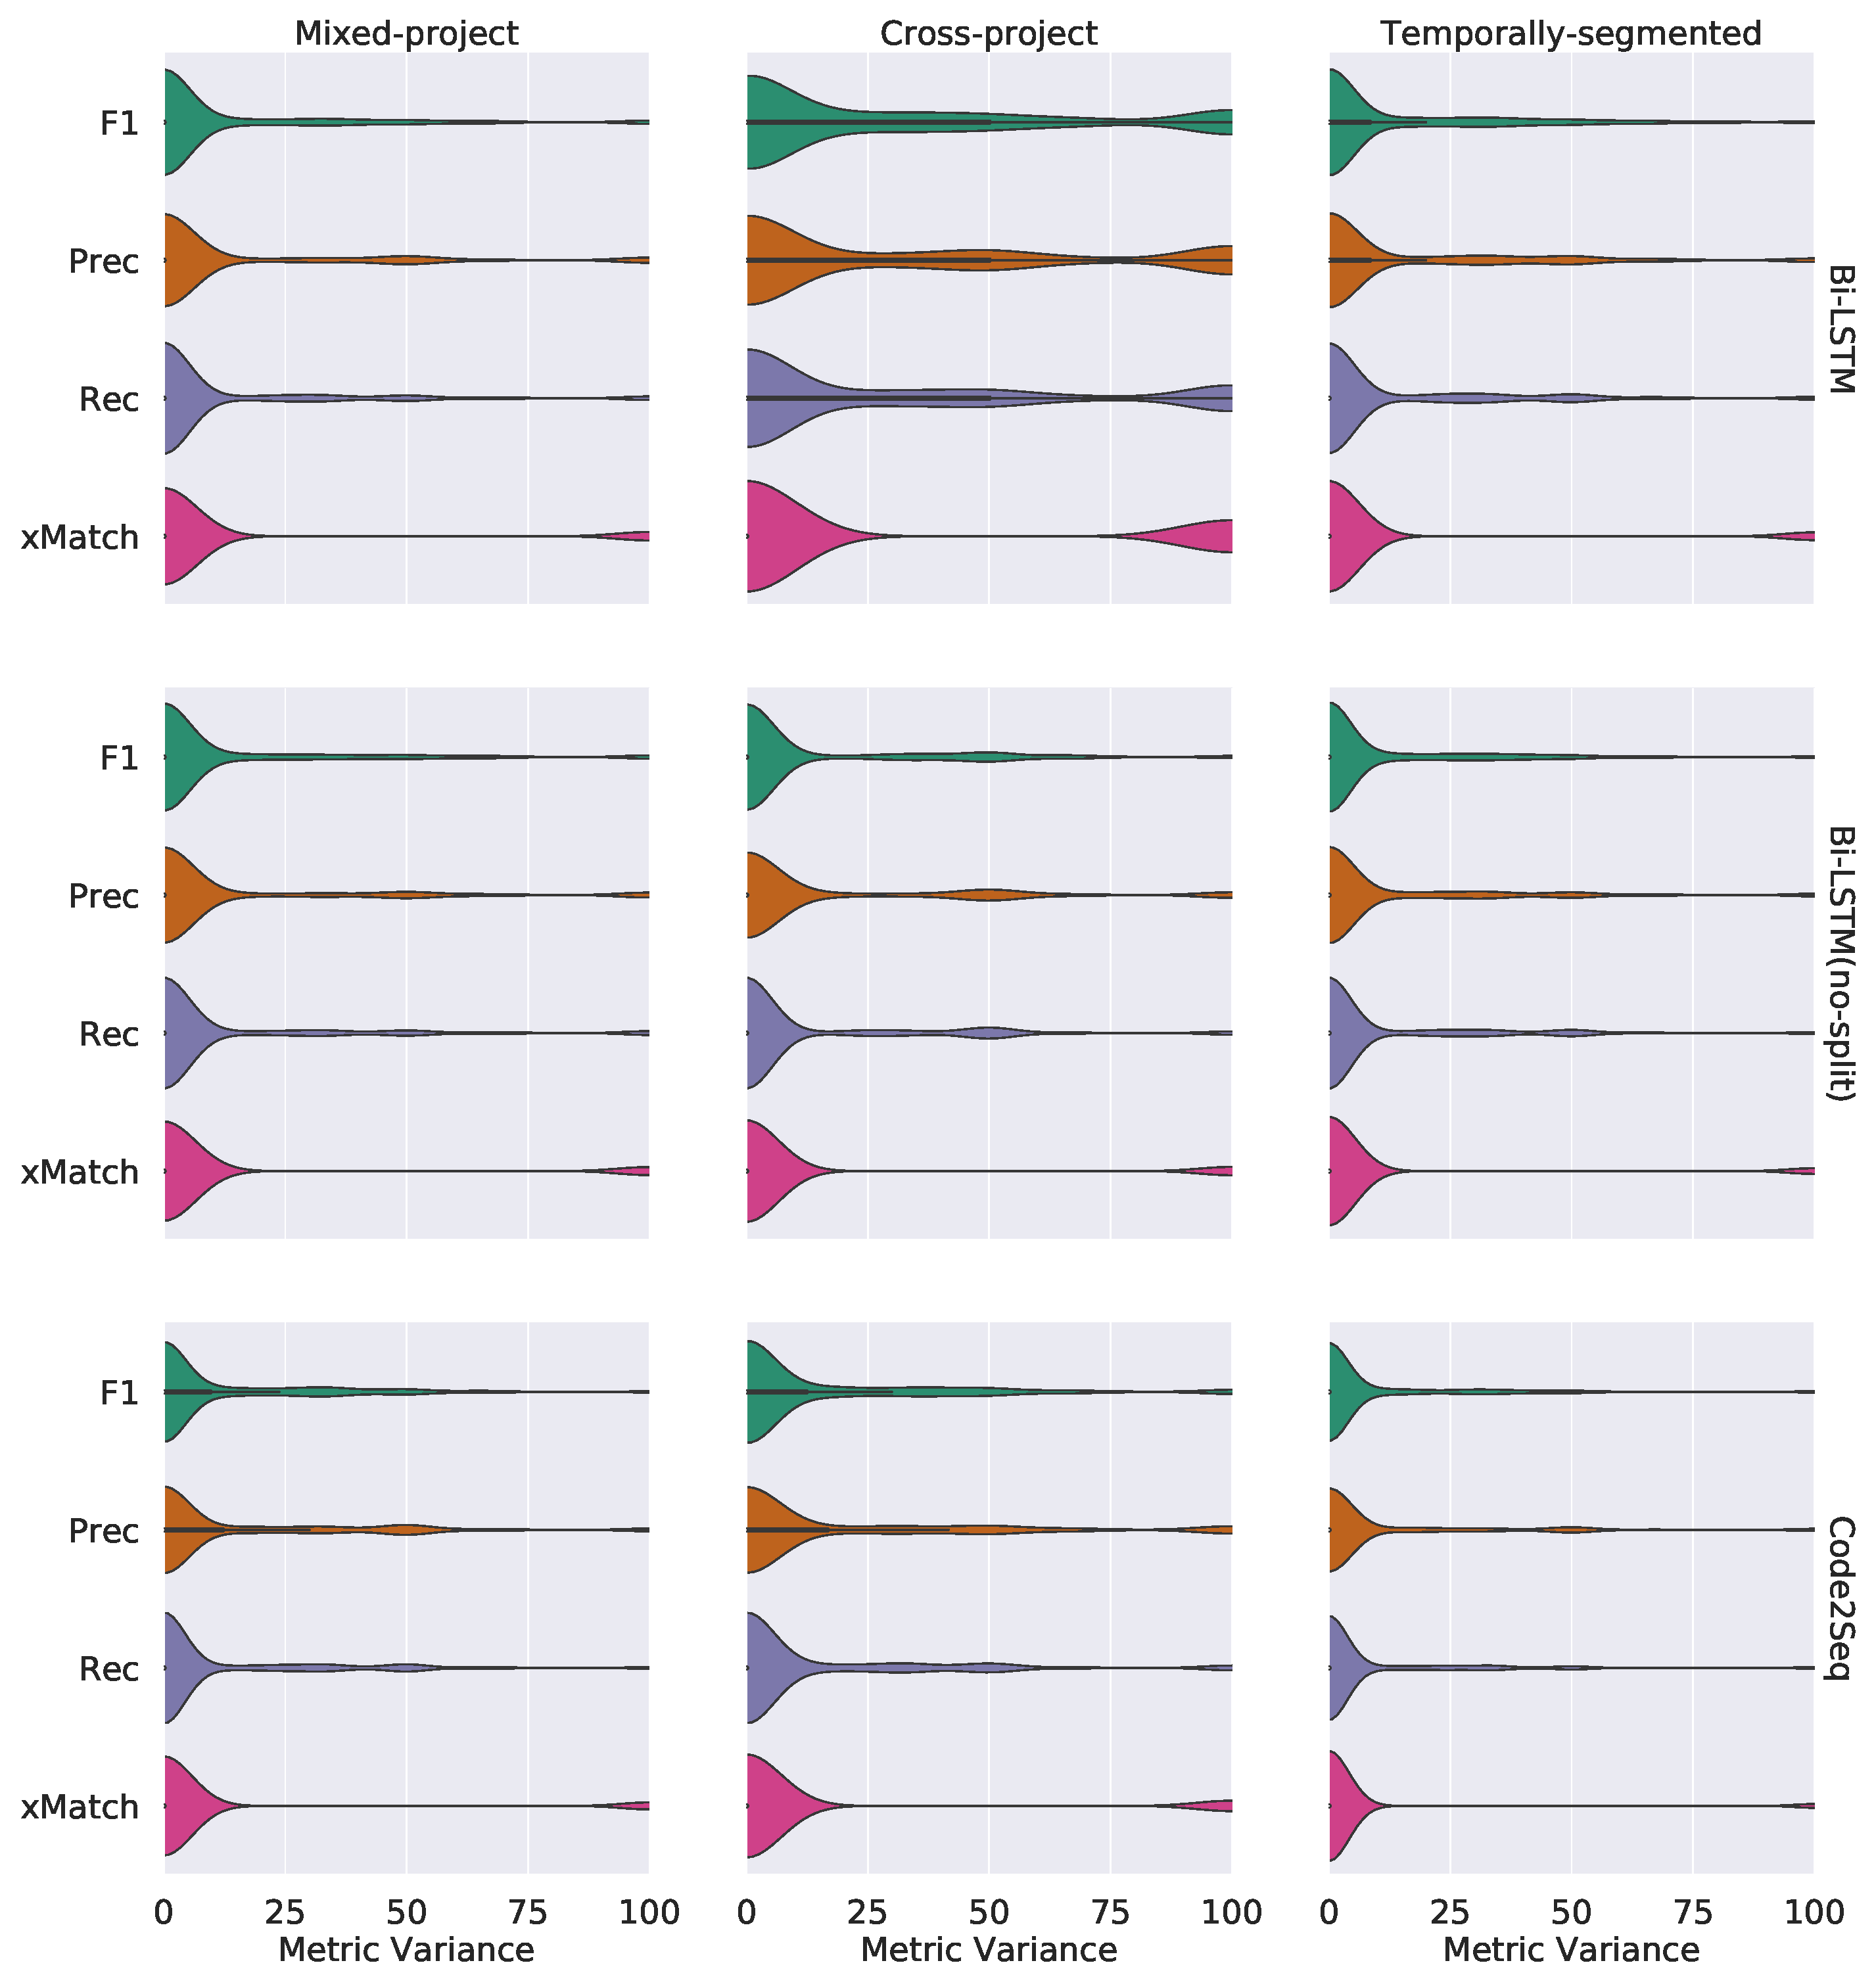
\includegraphics[width=\columnwidth]{figs/models-results-variance-dist-MethNam.eps}
  \caption{Each violin plot shows the distribution of the variances of
    automated metrics on all examples in \test set across \NumTrial
    trials.  Left to right: \mixedproj, \crossproj, and \evoaware
    \methodologies.  Top to bottom: the models for \methnam
    task. \label{fig:models-results-variance-dist-MethNam}}
\end{figure}

Figure~\ref{fig:models-results-metrics-dist-MethNam} shows the
distributions of automatic metrics on examples in \test set.
Figure~\ref{fig:models-results-variance-dist-MethNam} shows the
distributions of the variances of automated metrics on examples in
\test between \NumTrial different trials, where the variance is
calculated as the diff of the maximum value in \NumTrial trials and
minimum value in \NumTrial trials.


\subsection{Findings}
\label{sec:eval:findings}
From Table~\ref{}, models trained using \mixedproj \methodology and
\evoaware \methodology perform better in both automatic metrics than
\crossproj \methodology. This is because the using \mixedproj and
\evoaware \methodology models can learn from the
existing method and comment pairs within the projects so that the
model is able to generate comments that have similar styles or follow
the same rules. It has been shown by prior work that it is tough for
models to generalize between projects. All the models using \mixedproj
\methodology have better performance than \evoaware \methodology
probably because of the difference in the size of training data.
%Contradicted with Hu et al. ~\cite{}, \DeepCom does not outperform 
%\Seq2seq and \Seq2seqAtt uniformly in all the settings. DeepCom does
%worse than two baselines in mixed and cross proj setting but best in
%temporally setting.


% ========== The following tables are old before 20200827. They'll be either updated, replaced with plots, or removed

%
%% Automatically generated by pyutil.latex 

\begin{table*}
\begin{small}
\begin{center}
\caption{DeepCom results}
\begin{tabular}{l | c}
\toprule
  &BLEU-4 \\
\midrule
2013-2014-train
 & \UseMacro{deepcom-1314-bleu}
\\
2014-2015-train
 & \UseMacro{deepcom-1415-bleu}
\\
2015-2016-train
 & \UseMacro{deepcom-1516-bleu}
\\
2016-2017-train
 & \UseMacro{deepcom-1617-bleu}
\\
2017-2018-train
 & \UseMacro{deepcom-1718-bleu}
\\
\bottomrule
\end{tabular}
\end{center}
\end{small}
\vspace{\TVDatasetMetrics}
\end{table*}

%\begin{table*}
\begin{small}
\begin{center}
\caption{Results for Transformer}
\begin{tabular}{l | l}

\toprule

Training-Test & BLEU-4 \\

\midrule

Latest-Latest(epoch-20) &
\UseMacro{tr-lat-lat} \\
\midrule

Evolution-Latest(epoch-3) &
\UseMacro{tr-evo-lat} \\
\midrule

Evolution-Evolution(epoch-3) &
\UseMacro{tr-evo-evo} \\
\midrule

Latest-Evolution(epoch-18) &
\UseMacro{tr-lat-evo} \\
\midrule

\bottomrule

\end{tabular}
\end{center}
\end{small}
\vspace{\TVModels}
\end{table*}

%\begin{table*}
\begin{small}
\begin{center}
\caption{10 Projects}
\begin{tabular}{l}
\toprule
Projects \\
\midrule
   apache-commons-collections \\
google-guava\\
google-auto\\
rackerlabs-blueflood\\
jenkinsci-jenkins\\
dynjs-dynjs\\
spring-projects-spring-boot\\
oracle-graal\\
ReactiveX-RxJava\\
square-retrofit\\
\bottomrule
\end{tabular}
\end{center}
\end{small}
\vspace{\TVDatasetMetrics}
\end{table*}


%% 
%% Automatically generated by pyutil.latex 

\begin{table*}
\begin{small}
\begin{center}
\caption{Dataset statistics large (1000 projects)}
\begin{tabular}{l | r r r r r r r r}
\toprule
  &2013 & 2014 & 2015 & 2016 & 2017 & 2018 & 2019 & 2020 \\
\midrule
num-methods
 & \UseMacro{large-2013_Jan_1-num-methods}
 & \UseMacro{large-2014_Jan_1-num-methods}
 & \UseMacro{large-2015_Jan_1-num-methods}
 & \UseMacro{large-2016_Jan_1-num-methods}
 & \UseMacro{large-2017_Jan_1-num-methods}
 & \UseMacro{large-2018_Jan_1-num-methods}
 & \UseMacro{large-2019_Jan_1-num-methods}
 & \UseMacro{large-2020_Jan_1-num-methods}
\\
num-projs
 & \UseMacro{large-2013_Jan_1-num-projs}
 & \UseMacro{large-2014_Jan_1-num-projs}
 & \UseMacro{large-2015_Jan_1-num-projs}
 & \UseMacro{large-2016_Jan_1-num-projs}
 & \UseMacro{large-2017_Jan_1-num-projs}
 & \UseMacro{large-2018_Jan_1-num-projs}
 & \UseMacro{large-2019_Jan_1-num-projs}
 & \UseMacro{large-2020_Jan_1-num-projs}
\\
delta
 & \UseMacro{large-2013_Jan_1-delta}
 & \UseMacro{large-2014_Jan_1-delta}
 & \UseMacro{large-2015_Jan_1-delta}
 & \UseMacro{large-2016_Jan_1-delta}
 & \UseMacro{large-2017_Jan_1-delta}
 & \UseMacro{large-2018_Jan_1-delta}
 & \UseMacro{large-2019_Jan_1-delta}
 & \UseMacro{large-2020_Jan_1-delta}
\\
 after-filtered
 & N/A
 & \UseMacro{large-2013_Jan_1-2014_Jan_1-num-methods}
 & \UseMacro{large-2014_Jan_1-2015_Jan_1-num-methods}
 & \UseMacro{large-2015_Jan_1-2016_Jan_1-num-methods}
 & \UseMacro{large-2016_Jan_1-2017_Jan_1-num-methods}
 & \UseMacro{large-2017_Jan_1-2018_Jan_1-num-methods}
 & \UseMacro{large-2018_Jan_1-2019_Jan_1-num-methods}
 & \UseMacro{large-2019_Jan_1-2020_Jan_1-num-methods}
\\
\bottomrule
\end{tabular}
\end{center}
\end{small}
\vspace{\TVDatasetMetrics}
\end{table*}

%% 
%% Automatically generated by pyutil.latex 

\begin{table*}
\begin{small}
\begin{center}
\caption{Dataset statistics (10 projects)}
\begin{tabular}{l | r r r r r r r r}
\toprule
  &2013 & 2014 & 2015 & 2016 & 2017 & 2018 & 2019 & 2020 \\
\midrule
num-methods
 & \UseMacro{2013_Jan_1-num-methods}
 & \UseMacro{2014_Jan_1-num-methods}
 & \UseMacro{2015_Jan_1-num-methods}
 & \UseMacro{2016_Jan_1-num-methods}
 & \UseMacro{2017_Jan_1-num-methods}
 & \UseMacro{2018_Jan_1-num-methods}
 & \UseMacro{2019_Jan_1-num-methods}
 & \UseMacro{2020_Jan_1-num-methods}
\\
num-projs
 & \UseMacro{2013_Jan_1-num-projs}
 & \UseMacro{2014_Jan_1-num-projs}
 & \UseMacro{2015_Jan_1-num-projs}
 & \UseMacro{2016_Jan_1-num-projs}
 & \UseMacro{2017_Jan_1-num-projs}
 & \UseMacro{2018_Jan_1-num-projs}
 & \UseMacro{2019_Jan_1-num-projs}
 & \UseMacro{2020_Jan_1-num-projs}
\\
delta
 & \UseMacro{2013_Jan_1-delta}
 & \UseMacro{2014_Jan_1-delta}
 & \UseMacro{2015_Jan_1-delta}
 & \UseMacro{2016_Jan_1-delta}
 & \UseMacro{2017_Jan_1-delta}
 & \UseMacro{2018_Jan_1-delta}
 & \UseMacro{2019_Jan_1-delta}
 & \UseMacro{2020_Jan_1-delta}
\\
after-filtered
 & N/A
 & 4681
 & 3133
 & 5733
 & 6255
 & 9770
 & 6047
 & 6655
\\
\bottomrule
\end{tabular}
\end{center}
\end{small}
\vspace{\TVDatasetMetrics}
\end{table*}

%% 
%% Automatically generated by pyutil.latex 

\begin{table*}
\begin{small}
\begin{center}
\caption{method statistics after filtering (1000 projects)}
\begin{tabular}{l | c c c c c c c}
\toprule
 
 &
num-methods 
 &
len-avg 
 &
len-mode 
 &
len-median 
 &
len<100 
 &
len<150 
 &
len<200 
 \\
\midrule
2013-2014
 & \UseMacro{large-2013_Jan_1-2014_Jan_1-num-methods}
 & \UseMacro{large-2013_Jan_1-2014_Jan_1-method-tokens-avg}
 & \UseMacro{large-2013_Jan_1-2014_Jan_1-method-tokens-mode}
 & \UseMacro{large-2013_Jan_1-2014_Jan_1-method-tokens-median}
 & \UseMacro{large-2013_Jan_1-2014_Jan_1-method-tokens-less-100}
 & \UseMacro{large-2013_Jan_1-2014_Jan_1-method-tokens-less-150}
 & \UseMacro{large-2013_Jan_1-2014_Jan_1-method-tokens-less-200}
\\
2014-2015
 & \UseMacro{large-2014_Jan_1-2015_Jan_1-num-methods}
 & \UseMacro{large-2014_Jan_1-2015_Jan_1-method-tokens-avg}
 & \UseMacro{large-2014_Jan_1-2015_Jan_1-method-tokens-mode}
 & \UseMacro{large-2014_Jan_1-2015_Jan_1-method-tokens-median}
 & \UseMacro{large-2014_Jan_1-2015_Jan_1-method-tokens-less-100}
 & \UseMacro{large-2014_Jan_1-2015_Jan_1-method-tokens-less-150}
 & \UseMacro{large-2014_Jan_1-2015_Jan_1-method-tokens-less-200}
\\
2015-2016
 & \UseMacro{large-2015_Jan_1-2016_Jan_1-num-methods}
 & \UseMacro{large-2015_Jan_1-2016_Jan_1-method-tokens-avg}
 & \UseMacro{large-2015_Jan_1-2016_Jan_1-method-tokens-mode}
 & \UseMacro{large-2015_Jan_1-2016_Jan_1-method-tokens-median}
 & \UseMacro{large-2015_Jan_1-2016_Jan_1-method-tokens-less-100}
 & \UseMacro{large-2015_Jan_1-2016_Jan_1-method-tokens-less-150}
 & \UseMacro{large-2015_Jan_1-2016_Jan_1-method-tokens-less-200}
\\
2016-2017
 & \UseMacro{large-2016_Jan_1-2017_Jan_1-num-methods}
 & \UseMacro{large-2016_Jan_1-2017_Jan_1-method-tokens-avg}
 & \UseMacro{large-2016_Jan_1-2017_Jan_1-method-tokens-mode}
 & \UseMacro{large-2016_Jan_1-2017_Jan_1-method-tokens-median}
 & \UseMacro{large-2016_Jan_1-2017_Jan_1-method-tokens-less-100}
 & \UseMacro{large-2016_Jan_1-2017_Jan_1-method-tokens-less-150}
 & \UseMacro{large-2016_Jan_1-2017_Jan_1-method-tokens-less-200}
\\
2017-2018
 & \UseMacro{large-2017_Jan_1-2018_Jan_1-num-methods}
 & \UseMacro{large-2017_Jan_1-2018_Jan_1-method-tokens-avg}
 & \UseMacro{large-2017_Jan_1-2018_Jan_1-method-tokens-mode}
 & \UseMacro{large-2017_Jan_1-2018_Jan_1-method-tokens-median}
 & \UseMacro{large-2017_Jan_1-2018_Jan_1-method-tokens-less-100}
 & \UseMacro{large-2017_Jan_1-2018_Jan_1-method-tokens-less-150}
 & \UseMacro{large-2017_Jan_1-2018_Jan_1-method-tokens-less-200}
\\
2018-2019
 & \UseMacro{large-2018_Jan_1-2019_Jan_1-num-methods}
 & \UseMacro{large-2018_Jan_1-2019_Jan_1-method-tokens-avg}
 & \UseMacro{large-2018_Jan_1-2019_Jan_1-method-tokens-mode}
 & \UseMacro{large-2018_Jan_1-2019_Jan_1-method-tokens-median}
 & \UseMacro{large-2018_Jan_1-2019_Jan_1-method-tokens-less-100}
 & \UseMacro{large-2018_Jan_1-2019_Jan_1-method-tokens-less-150}
 & \UseMacro{large-2018_Jan_1-2019_Jan_1-method-tokens-less-200}
\\
2019-2020
 & \UseMacro{large-2019_Jan_1-2020_Jan_1-num-methods}
 & \UseMacro{large-2019_Jan_1-2020_Jan_1-method-tokens-avg}
 & \UseMacro{large-2019_Jan_1-2020_Jan_1-method-tokens-mode}
 & \UseMacro{large-2019_Jan_1-2020_Jan_1-method-tokens-median}
 & \UseMacro{large-2019_Jan_1-2020_Jan_1-method-tokens-less-100}
 & \UseMacro{large-2019_Jan_1-2020_Jan_1-method-tokens-less-150}
 & \UseMacro{large-2019_Jan_1-2020_Jan_1-method-tokens-less-200}
\\
\bottomrule
\end{tabular}
\end{center}
\end{small}
\vspace{\TVDatasetMetrics}
\end{table*}

%% 
%% Automatically generated by pyutil.latex 

\begin{table*}
\begin{small}
\begin{center}
\caption{method statistics after filtering (10 projects)}
\begin{tabular}{l | c c c c c c c}
\toprule
 
 &
num-methods 
 &
len-avg 
 &
len-mode 
 &
len-median 
 &
len<100 
 &
len<150 
 &
len<200 
 \\
\midrule
2013-2014
 & \UseMacro{2013_Jan_1-2014_Jan_1-num-methods}
 & \UseMacro{2013_Jan_1-2014_Jan_1-method-tokens-avg}
 & \UseMacro{2013_Jan_1-2014_Jan_1-method-tokens-mode}
 & \UseMacro{2013_Jan_1-2014_Jan_1-method-tokens-median}
 & \UseMacro{2013_Jan_1-2014_Jan_1-method-tokens-less-100}
 & \UseMacro{2013_Jan_1-2014_Jan_1-method-tokens-less-150}
 & \UseMacro{2013_Jan_1-2014_Jan_1-method-tokens-less-200}
\\
2014-2015
 & \UseMacro{2014_Jan_1-2015_Jan_1-num-methods}
 & \UseMacro{2014_Jan_1-2015_Jan_1-method-tokens-avg}
 & \UseMacro{2014_Jan_1-2015_Jan_1-method-tokens-mode}
 & \UseMacro{2014_Jan_1-2015_Jan_1-method-tokens-median}
 & \UseMacro{2014_Jan_1-2015_Jan_1-method-tokens-less-100}
 & \UseMacro{2014_Jan_1-2015_Jan_1-method-tokens-less-150}
 & \UseMacro{2014_Jan_1-2015_Jan_1-method-tokens-less-200}
\\
2015-2016
 & \UseMacro{2015_Jan_1-2016_Jan_1-num-methods}
 & \UseMacro{2015_Jan_1-2016_Jan_1-method-tokens-avg}
 & \UseMacro{2015_Jan_1-2016_Jan_1-method-tokens-mode}
 & \UseMacro{2015_Jan_1-2016_Jan_1-method-tokens-median}
 & \UseMacro{2015_Jan_1-2016_Jan_1-method-tokens-less-100}
 & \UseMacro{2015_Jan_1-2016_Jan_1-method-tokens-less-150}
 & \UseMacro{2015_Jan_1-2016_Jan_1-method-tokens-less-200}
\\
2016-2017
 & \UseMacro{2016_Jan_1-2017_Jan_1-num-methods}
 & \UseMacro{2016_Jan_1-2017_Jan_1-method-tokens-avg}
 & \UseMacro{2016_Jan_1-2017_Jan_1-method-tokens-mode}
 & \UseMacro{2016_Jan_1-2017_Jan_1-method-tokens-median}
 & \UseMacro{2016_Jan_1-2017_Jan_1-method-tokens-less-100}
 & \UseMacro{2016_Jan_1-2017_Jan_1-method-tokens-less-150}
 & \UseMacro{2016_Jan_1-2017_Jan_1-method-tokens-less-200}
\\
2017-2018
 & \UseMacro{2017_Jan_1-2018_Jan_1-num-methods}
 & \UseMacro{2017_Jan_1-2018_Jan_1-method-tokens-avg}
 & \UseMacro{2017_Jan_1-2018_Jan_1-method-tokens-mode}
 & \UseMacro{2017_Jan_1-2018_Jan_1-method-tokens-median}
 & \UseMacro{2017_Jan_1-2018_Jan_1-method-tokens-less-100}
 & \UseMacro{2017_Jan_1-2018_Jan_1-method-tokens-less-150}
 & \UseMacro{2017_Jan_1-2018_Jan_1-method-tokens-less-200}
\\
2018-2019
 & \UseMacro{2018_Jan_1-2019_Jan_1-num-methods}
 & \UseMacro{2018_Jan_1-2019_Jan_1-method-tokens-avg}
 & \UseMacro{2018_Jan_1-2019_Jan_1-method-tokens-mode}
 & \UseMacro{2018_Jan_1-2019_Jan_1-method-tokens-median}
 & \UseMacro{2018_Jan_1-2019_Jan_1-method-tokens-less-100}
 & \UseMacro{2018_Jan_1-2019_Jan_1-method-tokens-less-150}
 & \UseMacro{2018_Jan_1-2019_Jan_1-method-tokens-less-200}
\\
2019-2020
 & \UseMacro{2019_Jan_1-2020_Jan_1-num-methods}
 & \UseMacro{2019_Jan_1-2020_Jan_1-method-tokens-avg}
 & \UseMacro{2019_Jan_1-2020_Jan_1-method-tokens-mode}
 & \UseMacro{2019_Jan_1-2020_Jan_1-method-tokens-median}
 & \UseMacro{2019_Jan_1-2020_Jan_1-method-tokens-less-100}
 & \UseMacro{2019_Jan_1-2020_Jan_1-method-tokens-less-150}
 & \UseMacro{2019_Jan_1-2020_Jan_1-method-tokens-less-200}
\\
\bottomrule
\end{tabular}
\end{center}
\end{small}
\vspace{\TVDatasetMetrics}
\end{table*}

%% 
%% Automatically generated by pyutil.latex 

\begin{table*}
\begin{small}
\begin{center}
\caption{comment statistics after filtering (1000 projects)}
\begin{tabular}{l | c c c c c c c}
\toprule
 
 &
num-methods 
 &
len-avg 
 &
len-mode 
 &
len-median 
 &
len<20 
 &
len<30 
 &
len<50 
 \\
\midrule
2013-2014
 & \UseMacro{large-2013_Jan_1-2014_Jan_1-num-methods}
 & \UseMacro{large-2013_Jan_1-2014_Jan_1-comment-tokens-avg}
 & \UseMacro{large-2013_Jan_1-2014_Jan_1-comment-tokens-mode}
 & \UseMacro{large-2013_Jan_1-2014_Jan_1-comment-tokens-median}
 & \UseMacro{large-2013_Jan_1-2014_Jan_1-comment-tokens-less-20}
 & \UseMacro{large-2013_Jan_1-2014_Jan_1-comment-tokens-less-30}
 & \UseMacro{large-2013_Jan_1-2014_Jan_1-comment-tokens-less-50}
\\
2014-2015
 & \UseMacro{large-2014_Jan_1-2015_Jan_1-num-methods}
 & \UseMacro{large-2014_Jan_1-2015_Jan_1-comment-tokens-avg}
 & \UseMacro{large-2014_Jan_1-2015_Jan_1-comment-tokens-mode}
 & \UseMacro{large-2014_Jan_1-2015_Jan_1-comment-tokens-median}
 & \UseMacro{large-2014_Jan_1-2015_Jan_1-comment-tokens-less-20}
 & \UseMacro{large-2014_Jan_1-2015_Jan_1-comment-tokens-less-30}
 & \UseMacro{large-2014_Jan_1-2015_Jan_1-comment-tokens-less-50}
\\
2015-2016
 & \UseMacro{large-2015_Jan_1-2016_Jan_1-num-methods}
 & \UseMacro{large-2015_Jan_1-2016_Jan_1-comment-tokens-avg}
 & \UseMacro{large-2015_Jan_1-2016_Jan_1-comment-tokens-mode}
 & \UseMacro{large-2015_Jan_1-2016_Jan_1-comment-tokens-median}
 & \UseMacro{large-2015_Jan_1-2016_Jan_1-comment-tokens-less-20}
 & \UseMacro{large-2015_Jan_1-2016_Jan_1-comment-tokens-less-30}
 & \UseMacro{large-2015_Jan_1-2016_Jan_1-comment-tokens-less-50}
\\
2016-2017
 & \UseMacro{large-2016_Jan_1-2017_Jan_1-num-methods}
 & \UseMacro{large-2016_Jan_1-2017_Jan_1-comment-tokens-avg}
 & \UseMacro{large-2016_Jan_1-2017_Jan_1-comment-tokens-mode}
 & \UseMacro{large-2016_Jan_1-2017_Jan_1-comment-tokens-median}
 & \UseMacro{large-2016_Jan_1-2017_Jan_1-comment-tokens-less-20}
 & \UseMacro{large-2016_Jan_1-2017_Jan_1-comment-tokens-less-30}
 & \UseMacro{large-2016_Jan_1-2017_Jan_1-comment-tokens-less-50}
\\
2017-2018
 & \UseMacro{large-2017_Jan_1-2018_Jan_1-num-methods}
 & \UseMacro{large-2017_Jan_1-2018_Jan_1-comment-tokens-avg}
 & \UseMacro{large-2017_Jan_1-2018_Jan_1-comment-tokens-mode}
 & \UseMacro{large-2017_Jan_1-2018_Jan_1-comment-tokens-median}
 & \UseMacro{large-2017_Jan_1-2018_Jan_1-comment-tokens-less-20}
 & \UseMacro{large-2017_Jan_1-2018_Jan_1-comment-tokens-less-30}
 & \UseMacro{large-2017_Jan_1-2018_Jan_1-comment-tokens-less-50}
\\
2018-2019
 & \UseMacro{large-2018_Jan_1-2019_Jan_1-num-methods}
 & \UseMacro{large-2018_Jan_1-2019_Jan_1-comment-tokens-avg}
 & \UseMacro{large-2018_Jan_1-2019_Jan_1-comment-tokens-mode}
 & \UseMacro{large-2018_Jan_1-2019_Jan_1-comment-tokens-median}
 & \UseMacro{large-2018_Jan_1-2019_Jan_1-comment-tokens-less-20}
 & \UseMacro{large-2018_Jan_1-2019_Jan_1-comment-tokens-less-30}
 & \UseMacro{large-2018_Jan_1-2019_Jan_1-comment-tokens-less-50}
\\
2019-2020
 & \UseMacro{large-2019_Jan_1-2020_Jan_1-num-methods}
 & \UseMacro{large-2019_Jan_1-2020_Jan_1-comment-tokens-avg}
 & \UseMacro{large-2019_Jan_1-2020_Jan_1-comment-tokens-mode}
 & \UseMacro{large-2019_Jan_1-2020_Jan_1-comment-tokens-median}
 & \UseMacro{large-2019_Jan_1-2020_Jan_1-comment-tokens-less-20}
 & \UseMacro{large-2019_Jan_1-2020_Jan_1-comment-tokens-less-30}
 & \UseMacro{large-2019_Jan_1-2020_Jan_1-comment-tokens-less-50}
\\
\bottomrule
\end{tabular}
\end{center}
\end{small}
\vspace{\TVDatasetMetrics}
\end{table*}

%% \input{tables/table-time-wise-filtered-comment-dataset-metrics.tex}
%% 
%% Automatically generated by pyutil.latex 

\begin{table*}
\begin{small}
\begin{center}
\caption{DeepCom results}
\begin{tabular}{l | c}
\toprule
  &BLEU-4 \\
\midrule
2013-2014-train
 & \UseMacro{deepcom-1314-bleu}
\\
2014-2015-train
 & \UseMacro{deepcom-1415-bleu}
\\
2015-2016-train
 & \UseMacro{deepcom-1516-bleu}
\\
2016-2017-train
 & \UseMacro{deepcom-1617-bleu}
\\
2017-2018-train
 & \UseMacro{deepcom-1718-bleu}
\\
\bottomrule
\end{tabular}
\end{center}
\end{small}
\vspace{\TVDatasetMetrics}
\end{table*}

%% 
%% Automatically generated by pyutil.latex 

\begin{table*}
\begin{small}
\begin{center}
\caption{DeepCom results}
\begin{tabular}{l | c | c |c |c |c}
\toprule
 Time-BLEU-4
& Seq2seq
& Seq2seqAtt
& DeepCom-SBT
& DeepCom-Preorder
& DeepCom
\\
\midrule
2013-2014-train
 & \UseMacro{seq2seq-1314-bleu}
 & \UseMacro{seq2seqatt-1314-bleu}
 & \UseMacro{deepcom-sbt-1314-bleu}
 & \UseMacro{deepcom-preorder-1314-bleu}
 & \UseMacro{deepcom-1314-bleu}
\\
2014-2015-train
 & \UseMacro{seq2seq-1415-bleu}
 & \UseMacro{seq2seqatt-1415-bleu}
 & \UseMacro{deepcom-sbt-1415-bleu}
 & \UseMacro{deepcom-preorder-1415-bleu}
 & \UseMacro{deepcom-1415-bleu}
\\
2015-2016-train
 & \UseMacro{seq2seq-1516-bleu}
 & \UseMacro{seq2seqatt-1516-bleu}
 & \UseMacro{deepcom-sbt-1516-bleu}
 & \UseMacro{deepcom-preorder-1516-bleu}
 & \UseMacro{deepcom-1516-bleu}
\\
2016-2017-train
 & \UseMacro{seq2seq-1617-bleu}
 & \UseMacro{seq2seqatt-1617-bleu}
 & \UseMacro{deepcom-sbt-1617-bleu}
 & \UseMacro{deepcom-preorder-1617-bleu}
 & \UseMacro{deepcom-1617-bleu}
\\
2017-2018-train
 & \UseMacro{seq2seq-1718-bleu}
 & \UseMacro{seq2seqatt-1718-bleu}
 & \UseMacro{deepcom-sbt-1718-bleu}
 & \UseMacro{deepcom-preorder-1718-bleu}
 & \UseMacro{deepcom-1718-bleu}
\\
\bottomrule
\end{tabular}
\end{center}
\end{small}
\vspace{\TVDatasetMetrics}
\end{table*}

%% 
%% Automatically generated by pyutil.latex

\begin{table*}
\begin{small}
\begin{center}
\caption{DeepCom results on latest data}
\begin{tabular}{l | c | c |c |c |c}
\toprule
 Time-BLEU-4
& Seq2seq
& Seq2seqAtt
& DeepCom-SBT
& DeepCom-Preorder
& DeepCom
\\
\midrule
2020-train
 & 23.67
 & 24.17
 & 11.71
 & 8.15
 & 25.27
\\
\bottomrule
\end{tabular}
\end{center}
\end{small}
\vspace{\TVDatasetMetrics}
\end{table*}
%% 
%% Automatically generated by pyutil.latex 

\begin{table*}
\begin{small}
\begin{center}
\caption{Method naming statistics after filtering}
\begin{tabular}{l | c | c}
\toprule
 
 &
num-methods
&
code-len-avg
 \\
\midrule
2013-2014
 & \UseMacro{debug-beta-2013_Jan_1-2014_Jan_1-num-methods}
 & \UseMacro{debug-beta-2013-avg-len}
\\
2014-2015
 & \UseMacro{debug-beta-2014_Jan_1-2015_Jan_1-num-methods}
& \UseMacro{debug-beta-2014-avg-len}
\\
2015-2016
 & \UseMacro{debug-beta-2015_Jan_1-2016_Jan_1-num-methods}
& \UseMacro{debug-beta-2015-avg-len}
\\
2016-2017
 & \UseMacro{debug-beta-2016_Jan_1-2017_Jan_1-num-methods}
& \UseMacro{debug-beta-2016-avg-len}
\\
2017-2018
 & \UseMacro{debug-beta-2017_Jan_1-2018_Jan_1-num-methods}
& \UseMacro{debug-beta-2017-avg-len}
\\
2018-2019
 & \UseMacro{debug-beta-2018_Jan_1-2019_Jan_1-num-methods}
& \UseMacro{debug-beta-2018-avg-len}
\\
2019-2020
 & \UseMacro{debug-beta-2019_Jan_1-2020_Jan_1-num-methods}
 & \UseMacro{debug-beta-2019-avg-len}
\\
\bottomrule
\end{tabular}
\end{center}
\end{small}
\vspace{\TVDatasetMetrics}
\end{table*}

%% %% Automatically generated by pyutil.latex

\begin{table*}
\begin{small}
\begin{center}
\caption{Method naming task results}
\begin{tabular}{l | c | c}
\toprule
 Time-F1
 & Code2Seq
 & BiLSTM
\\
\midrule
2013-2014-train
 & \UseMacro{code2seq-debug-1314-F1}
 & 0.57
\\
2014-2015-train
 & \UseMacro{code2seq-debug-1415-F1}
 & 0.55
\\
2015-2016-train
 & \UseMacro{code2seq-debug-1516-F1}
 & 0.65
\\
2016-2017-train
 & \UseMacro{code2seq-debug-1617-F1}
 & 0.63
\\
2017-2018-train
 & \UseMacro{code2seq-debug-1718-F1}
 & 0.65
\\
latest-train
 & \UseMacro{code2seq-debug-latest-F1}
 & 0.58
\\
\bottomrule
\end{tabular}
\end{center}
\end{small}
\vspace{\TVDatasetMetrics}
\end{table*}

%% 
%% Automatically generated by pyutil.latex 

\begin{table*}
\begin{small}
\begin{center}
\caption{Comment-generation results}
\begin{tabular}{l|c|c|c|c}
\toprule
 Time-Bleu-4
& Seq2seq
& Seq2seqAtt
& DeepCom-SBT
& DeepCom
\\
\midrule
2013-2014-train
 & \UseMacro{seq2seq-1314-train-bleu}
 & \UseMacro{seq2seqatt-1314-train-bleu}
 & \UseMacro{deepcom-sbt-1314-train-bleu}
 & \UseMacro{deepcom-1314-train-bleu}
\\
2014-2015-train
 & \UseMacro{seq2seq-1415-train-bleu}
 & \UseMacro{seq2seqatt-1415-train-bleu}
 & \UseMacro{deepcom-sbt-1415-train-bleu}
 & \UseMacro{deepcom-1415-train-bleu}
\\
2015-2016-train
 & \UseMacro{seq2seq-1516-train-bleu}
 & \UseMacro{seq2seqatt-1516-train-bleu}
 & \UseMacro{deepcom-sbt-1516-train-bleu}
 & \UseMacro{deepcom-1516-train-bleu}
\\
2016-2017-train
 & \UseMacro{seq2seq-1617-train-bleu}
 & \UseMacro{seq2seqatt-1617-train-bleu}
 & \UseMacro{deepcom-sbt-1617-train-bleu}
 & \UseMacro{deepcom-1617-train-bleu}
\\
2017-2018-train
 & \UseMacro{seq2seq-1718-train-bleu}
 & \UseMacro{seq2seqatt-1718-train-bleu}
 & \UseMacro{deepcom-sbt-1718-train-bleu}
 & \UseMacro{deepcom-1718-train-bleu}
\\
2020-train
 & \UseMacro{seq2seq-latest-bleu}
 & \UseMacro{seq2seqatt-latest-bleu}
 & \UseMacro{deepcom-sbt-latest-bleu}
 & \UseMacro{deepcom-latest-bleu}
\\
\bottomrule
\end{tabular}
\end{center}
\end{small}
\vspace{\TVDatasetMetrics}
\end{table*}

%% 
%% Automatically generated by pyutil.latex 

\begin{table*}
\begin{small}
\begin{center}
\caption{Method-naming results}
\begin{tabular}{l|c|c|c|c|c|c|c|c|c}
\toprule
 \multirow{2}{*}{Time-Metrics}
& \multicolumn{3}{c}{Bi-LSTM}
& \multicolumn{3}{c}{no-split-Bi-LSTM}
& \multicolumn{3}{c}{Code2Seq}
\\
& precision
& recall
& f1
& precision
& recall
& f1
& precision
& recall
& f1
\\
\midrule
2013-2014-train
 & \UseMacro{bi-lstm-1314-train-precision}
 & \UseMacro{bi-lstm-1314-train-recall}
 & \UseMacro{bi-lstm-1314-train-f1}
 & \UseMacro{no-split-bi-lstm-1314-train-precision}
 & \UseMacro{no-split-bi-lstm-1314-train-recall}
 & \UseMacro{no-split-bi-lstm-1314-train-f1}
 & \UseMacro{code2seq-1314-train-precision}
 & \UseMacro{code2seq-1314-train-recall}
 & \UseMacro{code2seq-1314-train-f1}
\\
2014-2015-train
 & \UseMacro{bi-lstm-1415-train-precision}
 & \UseMacro{bi-lstm-1415-train-recall}
 & \UseMacro{bi-lstm-1415-train-f1}
 & \UseMacro{no-split-bi-lstm-1415-train-precision}
 & \UseMacro{no-split-bi-lstm-1415-train-recall}
 & \UseMacro{no-split-bi-lstm-1415-train-f1}
 & \UseMacro{code2seq-1415-train-precision}
 & \UseMacro{code2seq-1415-train-recall}
 & \UseMacro{code2seq-1415-train-f1}
\\
2015-2016-train
 & \UseMacro{bi-lstm-1516-train-precision}
 & \UseMacro{bi-lstm-1516-train-recall}
 & \UseMacro{bi-lstm-1516-train-f1}
 & \UseMacro{no-split-bi-lstm-1516-train-precision}
 & \UseMacro{no-split-bi-lstm-1516-train-recall}
 & \UseMacro{no-split-bi-lstm-1516-train-f1}
 & \UseMacro{code2seq-1516-train-precision}
 & \UseMacro{code2seq-1516-train-recall}
 & \UseMacro{code2seq-1516-train-f1}
\\
2016-2017-train
 & \UseMacro{bi-lstm-1617-train-precision}
 & \UseMacro{bi-lstm-1617-train-recall}
 & \UseMacro{bi-lstm-1617-train-f1}
 & \UseMacro{no-split-bi-lstm-1617-train-precision}
 & \UseMacro{no-split-bi-lstm-1617-train-recall}
 & \UseMacro{no-split-bi-lstm-1617-train-f1}
 & \UseMacro{code2seq-1617-train-precision}
 & \UseMacro{code2seq-1617-train-recall}
 & \UseMacro{code2seq-1617-train-f1}
\\
2017-2018-train
 & \UseMacro{bi-lstm-1718-train-precision}
 & \UseMacro{bi-lstm-1718-train-recall}
 & \UseMacro{bi-lstm-1718-train-f1}
 & \UseMacro{no-split-bi-lstm-1718-train-precision}
 & \UseMacro{no-split-bi-lstm-1718-train-recall}
 & \UseMacro{no-split-bi-lstm-1718-train-f1}
 & \UseMacro{code2seq-1718-train-precision}
 & \UseMacro{code2seq-1718-train-recall}
 & \UseMacro{code2seq-1718-train-f1}
\\
latest-mixed
 & \UseMacro{bi-lstm-latest-precision}
 & \UseMacro{bi-lstm-latest-recall}
 & \UseMacro{bi-lstm-latest-f1}
 & \UseMacro{no-split-bi-lstm-latest-precision}
 & \UseMacro{no-split-bi-lstm-latest-recall}
 & \UseMacro{no-split-bi-lstm-latest-f1}
 & \UseMacro{code2seq-latest-precision}
 & \UseMacro{code2seq-latest-recall}
 & \UseMacro{code2seq-latest-f1}
\\
latest-cross-project
 & \UseMacro{bi-lstm-cross-proj-latest-precision}
 & \UseMacro{bi-lstm-cross-proj-latest-recall}
 & \UseMacro{bi-lstm-cross-proj-latest-f1}
 & \UseMacro{no-split-bi-lstm-cross-proj-latest-precision}
 & \UseMacro{no-split-bi-lstm-cross-proj-latest-recall}
 & \UseMacro{no-split-bi-lstm-cross-proj-latest-f1}
 & \UseMacro{code2seq-cross-proj-latest-precision}
 & \UseMacro{code2seq-cross-proj-latest-recall}
 & \UseMacro{code2seq-cross-proj-latest-f1}
\\
\bottomrule
\end{tabular}
\end{center}
\end{small}
\vspace{\TVDatasetMetrics}
\end{table*}


\section{Threats to Validity}
\label{sec:threats}

\MyPara{Projects selection}

\MyPara{Programming languages selection}

\MyPara{Models selection}

\MyPara{Reproducibility of prior work}

\MyPara{Uncertainties of ML models}

\MyPara{Controlled experiment}

\section{Related Work}
\label{sec:related}

Tu et al.~\cite{TuETAL18Careful} revealed the data leakage problem
when using issue tracking data in the literature, caused by the
unawareness of the evolution of issue attributes.  We revealed that
similar problem also exists in the naturalness of software when using
code base data caused by the unawareness of the evolution of code, and
we propose practical and generalizable solutions to evaluate ML
techniques in evolution-aware settings to mitigate the threats of data
leakage.

\cite{BiswasAndRajan20Machine}

\subsection{Code Summarization}

%% \begin{table*}
\begin{small}
\begin{center}
\caption{\TCModels}
\begin{tabular}{l | l | l | l}

\toprule

Model & \makecell{Target\\Language} & Inputs & Code \\

\midrule

Iyer et al.~\cite{IyerETAL16Summarizing} CODE-NN &
\Csharp SQL &
code snippets &
\href{https://github.com/sriniiyer/codenn}{[Torch]} \\
\midrule

Liang and Zhu et al.~\cite{LiangAndZhu18Automatic} Tree-LSTM-GRU &
Java &
AST(exclude method names and params) &
\href{https://github.com/liang2024086/code_comment_generation}{[Tensorflow]} \\
\midrule

Wan et al.~\cite{WanETAL18Improving} Code-RL &
Python &
AST+code snippets &
\href{https://github.com/wanyao1992/code_Summarization_public}{[Pytorch]} \\
\midrule

Hu et al.~\cite{HuETAL18Deep} DeepCom &
Java &
SBT+code snippets &
\href{https://github.com/xing-hu/EMSE-DeepCom}{[Tensorflow]} \\
\midrule

Hu et al.~\cite{HuETAL18Summarizing} TL-CodeSum &
Java &
api sequence+code snippets &
\href{https://github.com/xing-hu/TL-CodeSum}{[Tensorflow]} \\
\midrule

LeClair et al.~\cite{LeClairETAL19Neural} ast-attendgru &
Java &
AST+code snippets &
\href{https://s3.us-east-2.amazonaws.com/icse2018/index.html}{[Keras]} \\
\midrule

Alon et al.~\cite{AlonETAL19code2seq} code2seq &
Java &
AST paths &
\href{https://github.com/m3yrin/code2seq}{[Pytorch]} \\
\midrule

Fernandes et al.~\cite{FernandesETAL19Structured} BiLSTM+GNN &
Java &
graph representation of code &
\href{https://github.com/CoderPat/structured-neural-summarization}{[Tensorflow]}\\
\midrule

LeClair et al.~\cite{LeClairETAL20Improved} code+gnn+BiLSTM &
Java &
AST+code snippets &
\href{https://github.com/acleclair/ICPC2020_GNN}{[Tensorflow+Keras]} \\
\midrule

\bottomrule

\end{tabular}
\end{center}
\end{small}
\vspace{\TVModels}
\end{table*}

Most of the neural comment generation work
frame the task as a encoder-decoder structure
and generate comments from source code. The mainstream
approaches can be categorized into textual-based approach,
structure-based approach and hybrid approach.

The textual-based approaches only consider the sequential
information in the code sequence.
Iyer et al.\cite{IyerETAL16Summarizing} use Long Short Term Memory
(LSTM) network with attention to produce summaries with given SQL
sequence. Allamanis et al.~\cite{AllamanisETAL16Convolutional} propose
to use convolutional attention network to summarize the input source
code. Ahmad et al.~\cite{AhmadETAL20Transformer-based} propose to use transformer equipped with relative positions representation and copy attention to generate comments.

The structure-based approaches mostly takes the structure of source code
into consideration.
Hu et al.~\cite{HuETAL18Deep} develop a novel traversal
method ``Structure-Based Traversal'' to first flatten the Abstract
Syntax Tree (AST) into sequence as the input of encoder.
Liang et al.~\cite{LiangAndZhu18Automatic} use Recursive Neural
Network to directly encode the AST of code snippets. Alon et
al.~\cite{AlonETAL19code2seq} extract AST paths
(path between two terminals in AST) from code and uniformly sample to
get the inputs of LSTM encoder. Fernandes et
al.~\cite{FernandesETAL19Structured} first represent code with graph
following the way proposed by Allamanis et
al.~\cite{AllamanisETAL18Learning}
and use both Gated Graph Neural Network (GGNN) and biLSTM to learn the graph representation.

The hybrid approaches usually use more than one modality to help
generate comments. Hu et al.~\cite{HuETAL19Deep} propose a model to
encode SBT sequence and code sequence separately with separate
attention which shows improvement over the AST based
approach~\cite{HuETAL18Summarizing}. LeClair et
al.~\cite{LeClairETAL20Improved} use a Graph Neural Network to learn
the AST representation rather than directly using flattened AST
sequence.

In addition to AST, other auxiliary information is used to help
comment generation. Hu et al.~\cite{HuETAL18Summarizing} extract and
encode API usage sequence from the source code to see further
improvement. Cai et al.~\cite{CaiETAL20TAG} incorporate the type of
AST node. They first build a Token-type-tree which is a
N-ary tree where each node is consisted of token from code sequence and the type of the corresponding AST node
from source code. Then they use tree-LSTM  encoder and decoder to
generate comments with the help of type information.

% (ICPC'18); Hu et al.~\cite{HuETAL19Deep}
% Based on \sts models, where encoder can take tree inputs by
%flattening them into sequences.  They essentially like this: ``(
%parent children ) parent''.  Handle OOV by backing-up to the AST
%type. Dataset is available.


%Iyer et al.~\cite{IyerETAL16Summarizing} use 
%(ACL'16). CODE-NN, used
%Long Short Term Memory (LSTM) networks with attention to produce summaries
%of \Csharp and SQL based on the code snippet.
%Dataset is from Stack Overflow.

%Loyola et al.~\cite{LoyolaETAL17Neural} (ACL'17). Used seq2seq model
%trained on code changes to generate commit messages.  Dataset is 12
%real-world repositories. Language: python, javascript, c++, java.


%Liang and Zhu~\cite{LiangAndZhu18Automatic}% (AAAI'18)
%take advantage of the structure information of programming language
%and use Recursive NN (tree-lstm) to encode
%the AST of code snippets.
%They added 'CombineName' node which indicates sub-tokenizing
%the identifiers. Then used the learned representation of ast as the input of GRU decoder.
%They studied Java, and used ten open-source Java code repos from Github. 
%Used ten open-source Java code repositories from
%GitHub for this experiment. In each of these
%repositories they extracted descriptive comment and the corresponding method pairs.
%Constructor methods are excluded from this exercise. These pairs are then used for
%training and test. \textbf{Notice that all the method names and
%parameters are excluded from training and test.}
%\textbf{Code}: [Tensorflow] \url{https://github.com/liang2024086/code_comment_generation}

%Reinforcement learning is also applied to this area, Wan et
%al.~\cite{WanETAL18Improving} %(ASE'18).
%incorporate AST as well as sequential content of code snippets into a deep reinforcement learning framework
%(i.e., actor-critic network). The actor network provides the confidence
%of predicting the next word according to current state. The critic network
%evaluates the reward value of all possible extensions of the current state and
%can provide global guidance for explorations.
%They employ an advantage reward composed of BLEU metric to train both networks.

%Studied python, used datasets from~\cite{BaroneAndSennrich17Parallel}
%The experiments are done with Python.
%To construct the tree-structure of code, they parse Python code into
%abstract syntax trees via ast2 lib. To convert code into sequential
%text, they tokenize the code by some special tokens.  They also tokenize the comment by {(space)}.
%``{. , ” ’ : ; ) ( ! (space)}. 
%\textbf{Code}: [Pytorch] \url{https://github.com/wanyao1992/code_Summarization_public}

%% Hu et al.~\cite{HuETAL18Deep}% (ICPC'18); Hu et al.~\cite{HuETAL19Deep}
%% (ESE'19).  Based on \sts models, where encoder can take tree inputs by
%% flattening them into sequences.  They developed a novel flattening
%% method ``Structure-Based Traversal'', essentially like this: ``(
%% parent children ) parent''.  Handle OOV by backing-up to the AST
%% type. Dataset is available.
%To decrease noise introduced to the
%learning process, they only take the first sentence of the comments%
%since they typically describe the functionalities of Java methods
%according to Javadoc guidance2 . However, not every comment is useful.
%Methods with empty or just one-word descriptions are filtered out in
%this work. The setter, getter, constructor, test methods, and override
%methods, whose comments are easy to predict, are also excluded.
%\textbf{Code}: [Tensorflow]
%\url{https://github.com/xing-hu/EMSE-DeepCom}

%% The BLEU scores reported in Hu et al.~\cite{HuETAL18Deep} could not be
%% replicated as pointed out by Alon et al.~\cite{AlonETAL19code2seq}.
%% This might be due to a different nltk library version they used, as we
%% observed the BLEU score computation in nltk library has been
%% dramatically changed in the history (e.g., version 3.2).



%% Hu et al.~\cite{HuETAL18Summarizing} (IJCAI'18). Use a code encoder and API encoder (pre-trained on
%% API summarization task) as inputs of decoder. (API sequence can be obtained from source code,
%% but the code used to extract not provided) 
%% Dataset is available.
%\textbf{Code}: [Tensorflow] \url{https://github.com/xing-hu/TL-CodeSum}
%Methods with empty or just one-word descriptions are filtered
%out in this work. The setter, getter, constructor, test methods,
%and override methods, whose comments are easy to predict,
%are also excluded.

%% LeClair et al.~\cite{LeClairETAL19Neural} (ICSE'19).  In addition to
%% the ``standard'' experiment of summarization from source code, they
%% also study the ``challenge'' experiment of summarization from bytecode
%% (using only AST of methods to generate comments). They create a multi-input model
%% that used the SBT sequence with all identifiers removed as the first
%% input, and the source code tokens as the second. They found that if
%% you decouple the structure of the code form the code itself that the
%% model improved its ability to learn that structure.
%% Dataset from
%% Sourcerer repository provided by Lopes et al. The repository contains
%% over 51 million Java methods from over 50000 projects.
%% They take out first sentence of Javadoc, filter out comments not in English,
%% using langdetect (\url{https://pypi.org/project/langdetect/}) remove
%% methods over 100 words long and comments >13 and <3 words they remove
%% any methods from files that include phrases such as ``generated by''.
%% This filter is quite aggressive, as it reduced the dataset size
%% to around 2m methods, and on manual inspection they found no cases of
%% autogenerated code. In fact, a majority of the filtered methods theyre
%% exact duplicates (around 100k unique examples out of \~2m removed
%% methods). But because comments to auto-generated code are often still
%% meaningful, they added one copy of each of the 100k unique examples back
%% into the dataset, and ensured that they theyre in the training set only
%% (so they did not attempt to test against auto-generated comments). The
%% result is a dataset of around 2.1m methods.  To obtain the ASTs, they
%% first used srcml (\url{https://ieeexplore.ieee.org/document/6065176})
%% to extract an XML representation of each method. Then they built a tool
%% to convert the XML representation into the flattened SBT
%% representation. they created our own modification of SBT in which all
%% the code structure remained intact, but in which they replaced all words
%% (except official Java API class names) in the code to a special
%% <OTHER> token. They call this SBT-AO for SBT AST only. They use this
%% modification to simulate the case when only an AST can be extracted.
%% \textbf{Code}: [Keres]
%% \url{https://s3.us-east-2.amazonaws.com/icse2018/index.html}

%% %LeClair and McMillan~\cite{LeClairAndMcMillan19Recommendations} (NAACL'19).
%% %This paper recommends people to use their dataset to do code summarization.
%% %The dataset includes 2.1m pairs of
%% %Java methods and \javadoc pairs over 28k Java projects.  Dataset based
%% %on their previous work~\cite{LeClairETAL19Neural}, rooted
%% %from~\cite{LopesETAL10UCI}.  Analyzed splitting by method
%% %v.s. splitting by project, and removing auto generated Java methods.
%% %Dataset can be downloaded: \url{http://leclair.tech/data/funcom/}

%% Alon et al.~\cite{AlonETAL19code2seq} (ICLR'19). They combine the uniformly sampled k
%% AST paths (path between two terminals in AST) and terminals' tokens as
%% inputs of decoder, then generate comments. Studied Java, use their own
%% datasets.  Java-large: new dataset of the 9500 top-starred Java
%% projects from GitHub that were created since January 2007. They randomly
%% select 9000 projects for training, 250 for validation and 300 for
%% testing. This dataset contains about 16M examples and it is publicly available.  \textbf{Code}: [Tensorflow]
%% \url{https://github.com/tech-srl/code2seq} [Pytorch]
%% \url{https://github.com/m3yrin/code2seq}

%% Fernandes et al.~\cite{FernandesETAL19Structured} (ICLR'19).  Experimented with GGNN
%% encoder and sequence+GGNN encoder.  Studied both \Csharp and Java,
%% used many datasets from various sources. Represent code with graph~\cite{AllamanisETAL18Learning}.
%% Dataset
%% from~\cite{AlonETAL19code2seq}. \textbf{Code}: [Tensorflow]
%% \url{https://github.com/CoderPat/structured-neural-summarization}

%% LeClair et al.~\cite{LeClairETAL20Improved} (ICPC'20).  Models based
%% on their previous work~\cite{LeClairETAL19Neural}.  Use a ConvGNN
%% rather than flattened AST in the multi-input \sts model.  Dataset
%% taken from their previous
%% work~\cite{LeClairAndMcMillan19Recommendations}.  Use the
%% SrcML(\url{https://www.srcml.org/}) library to generate the associated
%% ASTs from the raw source code.  \textbf{Code}: [Tensorflow+Keras]
%% \url{https://github.com/acleclair/ICPC2020_GNN}

%% Ahmad et al.~\cite{AhmadETAL20Transformer-based} (ACL'20).  They use a
%% transformer equipped with relative encoding of code tokens' positions
%% and copy mechanism.  They use a Java dataset (from Hu et
%% al.~\cite{HuETAL18Summarizing}) and Python dataset (from Barone and
%% Sennrich~\cite{BaroneAndSennrich17Parallel}).  \textbf{Code}:
%% [Pytorch] \url{https://github.com/wasiahmad/NeuralCodeSum}

%% Cai et al.~\cite{CaiETAL20TAG} (ACL'20).  \Fix{TODO}.

%% Zhao et al.~\cite{ZhaoETAL20Survey} is a survey of some (very old)
%% comment generation models.

\subsection{Evolution Data}
Tan et al.~\cite{TanETAL15Online} point out that using
cross-validation to train defect prediction classifier (predict
whether a change is buggy at the time of the commit) will use future
data which does not match a real-world usage scenario. Therefore they
propose time sensitive change classification which uses information,
known at time $t$ only, to classify change $c$ that is committed at $t$.
For example, time sensitive change classification predicts at time
$t_{predict}$ for the change $C_6$, i.e., the test set.  The changes
committed before $C_6$ are the training set, i.e., $C_1$-$C_5$, which
is used to build models.

Lutellier et al.~\cite{LutellierETAL20CoCoNut} propose a new technique
CoCoNuT, which uses ensemble learning on the combination of
convolutional neural networks (CNNs) and a new context-aware neural
machine translation (NMT) architecture to automatically fix bugs in
multiple programming languages. They claim they are the first to
acknowledge and address using-future-data threat in the context of
program repair techniques (APR).
They split benchmark into two parts The first part contains bugs from
2006 to 2010 and is used to evaluate CoCoNuT trained with data from
before 2006. The second part of the benchmark contains bugs from 2011
to 2016 and is used to evaluate CoCoNuT trained with data from before
2011 (including data from before 2006). This split allows CoCoNuT to
learn from instances up to 2010 to fix newer bugs while keeping the
overhead reasonable. They then combine the results of CoCoNuT on these
two sub-benchmarks to obtain the final number of bugs fixed. With this
correct setting, CoCoNuT has no access to data that would be
unavailable in a realistic scenario.

Pradel et al.~\cite{PradelETAL20Scaffle} present a bug localization
technique which is based on the key insight to divide the problem into
two easier sub-problems. First, a trained machine learning model
encodes the raw crash trace and predicts which lines of a raw crash
trace are most informative for localizing the bug. Then, these lines
are fed to an information retrieval-based search engine to retrieve
file paths in the code base, predicting which file to change to
address the crash.  To evaluate the system in a realistic setup, they
simulate using the approach at different points in time. At each point
in time $t$, they simulate by training its model based on all data
available at $t$ and by predicting the bug locations for all crash
traces that occur between $t$ and $t$ + 50 days.  For the prediction,
they gather the set of all files in the code base at $t$ + 50 days and
let the path prediction component predict which of these files need to
be fixed. This setup is realistic, as it uses only past data to
predict future bug locations

\input{conclusion}

%% \RevisionInfo

%% Acknowledgments
%\section*{Acknowledgment}


%% References
\bibliographystyle{IEEEtran}
\bibliography{bib}


%% Appendix
%% \clearpage
%% \newpage
%% \appendix
%% \section{Discussion Logs}

We document some important discussions here.

\subsection{20200521}

\begin{itemize}
\item We noticed that training on evolution set didn't improve a lot
  than training on latest set, though evolution set is $3 \sim 4
  \times$ bigger than latest set.  We were curious maybe increasing
  the set size doesn't help improving performance after some certain
  point.  We could do an experiment to test that.
\item For the purpose in the previous item, also to get better
  estimation on the final testing set performance, we think maybe in
  the small version of data set, testing set shouldn't be
  down-sampled.
\item For the next model to integrate, we agreed to prioritize recent
  architecture: GNN and transformer.
\end{itemize}


\subsection{20200525}

\begin{itemize}
\item We looked into several NLP papers (new model / comparison of
  models / critical evaluations) in order to not repeating some wrong
  paths and see what's the path that we want to take.  Below are a
  bunch of things that we can consider doing...
\item Do a critical evaluation over comment generation models.
\item Introduce a model that beats all other models simply by using
  more data - which will likely be a deep transformer model, which may
  be very soon be out-dated after other deeper model / larger data set
  comes out.
\item Study how to use data from project history.
\item Study how to use data from different quality projects.
\end{itemize}


\subsection{20200718}

Email threads:

\textbf{On June 19, Milos said:}

I still believe that the work we started on evaluating comment
generation is an excellent topic, and that work can be published at a
top conference.  However, there is one bigger question that I think we
should ask first:

How to properly evaluate NLP/ML techniques that target software

Prior work (including our original plan to include evolution data) looks
only at a single point in time and using all data available at that
point.  That seems conceptually broken.  I think (as I discussed with
Pengyu) that we need to take much closer look at how software (used in
the evaluations) evolves and what is available at each point.

Let me give an example.  Say that we want to generate comments at time
$t_n$.  (All published papers take into account code available in $t_n$,
split things based on files or projects and evaluate their approach.)
Here is what we should do:

Split each project history based in several time frames (frames for
short).  We want to use same frames for each project.  Let's say we have
the following frames:

f1 (2016), f2 (2017), f3 (2018), f4 (2019), f5 (2020)

Note that we do not need to define frame=year (this can be also month or
maybe even week or a day in the limit).

Then we would train models on data available at the end of f1 and use
that model to predict things in f2.  We would then train on f2 and use
that model to predict f3, etc.

My impression is currently that we should only use previous frame for
training (and not *all* previous frames); two reasons: (1) we do not
want training sets to overlap (although I am not sure about this one),
and (2) more recent data is likely to give better prediction (although
we have seen that more data even if noise can help).

We can apply this approach, we can call it time-aware (or time-shifted
or time-travel) to any NLP/ML approach that was studied in the past.
(Maybe those papers that do comment generation do take comments in
order; hopefully?  Can you please check.)  This includes work on comment
generation, comment update, code completion.  I feel that going with
code completion and comment generation can be simplest for now.

In short, I proposed that we focus on time-aware evolution of NLP/ML
models for SE for ICSE.

We can still keep that in the repo that you have (because it is related
to evolution) or we can make a new one.

This is doable for ICSE and can be very exciting topic.

Let me know if you have any questions.  If not, then we should start :)

We can start with the following:
use frame of 1 year
do comment generation (as you have some models running)

We can all other things as we go.


\textbf{On June 28, Milos said:}

I think Pengyu knows of this paper, which is the most relevant for our
planned work for ICSE:

\url{https://dl.acm.org/doi/10.1145/3236024.3236054} \cite{TuETAL18Careful}


\textbf{On July 4, Milos said:}

Inspired by some recent discussions with Pengyu, let me expand on our
plan for ICSE 2021.

We were originally thinking to evaluate on each commit.  That is still
great and we should do it!  ICSE is the best target.

Additionally, we can use PRs (both those that are accepted and rejected)
in our evaluation.  We can apply our approach to each PR and evaluate
the outcome (and even see if that correlates with PR being
rejected/accepted).  Definitely more things to think through, but
something to keep on the list.  We keep things up-to-date in that
evolution repo, right?


\subsection{20200725}

\textbf{Discussion: the finding of the ICSE'15
  paper~\cite{TanETAL15Online}}:

We don't think our work is less important because of this paper.
Several novel aspects:

\begin{itemize}
\item We are doing generative tasks, while existing work including
  Tan et al.~\cite{TanETAL15Online} is doing classification tasks (defect
  prediction).
\item Showing the results of recent popular techniques will be
  valuable.  For example, DeepCom, n-gram code completion
  (Naturalness), and one more would be good.
\item In Tan et al.~\cite{TanETAL15Online}, they go into another limit and claim
  that this time based approach is what is correct.  We would say both
  can be correct \textit{depending on the task}.  For example, a
  company may want to build a model now and apply to code from 2012 to
  find something or learn something about that code.  In other words,
  using future might not always be unfair and that has to be clearly
  stated in our paper.
\item Rather than having one performance score for a model on the
  dataset obtained in new version (usually removing duplicate data),
  it will also be useful to know the performance on some other
  subsets.  For example: (1) regression data (i.e., data existed in
  previous version); (2) new data, which can be split to \{cloned,
  trivial, novel\} new data; (3) the new data in the files/projects
  existed in previous version; (4) the new data not in the
  files/projects existed in previous version.
\end{itemize}

\textbf{Is cross-entropy computed in Naturalness paper is impacted?}

Pengyu: Naturalness paper primarily studied two things and one of them
is affected.  (1) They use cross-entropy as an indication of the
``naturalness'' of software at a specific revision - that is fine.
(2) They use n-gram language model built on a part of software to
apply on the rest - that is not fine and impacted by potential data
leakage.


%% Text of appendix \ldots

\end{document}
